\documentclass[a4paper,11pt]{article}
\usepackage{graphicx}
\usepackage{caption}
\usepackage{enumitem}
\usepackage{multicol}
\usepackage{mathtools}
\usepackage{hyperref}
\usepackage{amsmath,amsthm,amssymb,cancel,bm}
\usepackage{floatrow}
\setcounter{tocdepth}{2}
\usepackage{geometry}
\geometry{total={210mm,297mm},
left=25mm,right=25mm,%
bindingoffset=0mm, top=20mm,bottom=20mm}
\newcommand{\linia}{\rule{\linewidth}{0.5pt}}

% my own titles
\makeatletter
\renewcommand{\maketitle}{
\begin{center}
\vspace{2ex}
{\huge \textsc{\@title}}
\vspace{1ex}
\\
\linia\\
\@author
\vspace{4ex}
\end{center}
}
\makeatother

% custom footers and headers
\usepackage{fancyhdr,lastpage}
\pagestyle{fancy}
\lhead{}
\chead{}
\rhead{}
\renewcommand{\headrulewidth}{0pt}
\lfoot{General Qualifying Exam Solutions}
\cfoot{}
\rfoot{Page \thepage\ /\ \pageref*{LastPage}}

% --------------------------------------------------------------
%
%                           TITLE PAGE
%
% --------------------------------------------------------------

\begin{document}
\hfill{\textit{Last modified \today}}
\title{General Qualifying Exam Solutions: Cosmology}
\author{Jessica Campbell, Dunlap Institute for Astronomy \& Astrophysics (UofT)}
\date{\today}
\maketitle

\tableofcontents


% --------------------------------------------------------------
%
%
%                              COSMOLOGY 
%
%
% --------------------------------------------------------------

\newpage
\section{Cosmology}

\subsection{Preface}
Cosmology is the study of the Universe on the largest of scales -- the origin, evolution, and possible fate of the Universe as a whole. Cosmology concerns itself with asking questions such as: ``Where do we come from? What is the Universe made of? How did the elements form? Is it finite or infinite in spatial extent? Why is the Universe so smooth? How did galaxies form from such a smooth origin? Did the Universe have a beginning sometime in the past? Will it come to an end sometime in the future?'' As a branch of science that studies the entirety of the Universe, it often deals with distances that are very big, objects that are very large, and timescales that are very long. For this reason, standard units of distance (meters), mass (kilogram), and time (seconds or years) are far too small and therefore conventionally work in much larger standard units.

One distance measure often employed by astronomers is the \textbf{astronomical unit} (AU) which is the average distance between the Earth and the Sun over a period of one year: $1 {\rm AU} = 1.5 \times 10^{11}\,{\rm m}$. Such a distance scale is useful on the scale of the Solar System, but is small compared to the distance between stars. For interstellar distances, another unit of measure called the \textbf{parsec} (pc) is most useful which is defined to be the distance at which one AU subtends an angle of one arcsecond: $1\,{\rm pc} = 3.1\times10^{16}\,{\rm m}$. For example, we are located approximately $1.3\,{\rm pc}$ away from the nearest star, Proxima Centauri and $85\,{\rm pc}$ from the center of the Galaxy. This distance measure is therefore most useful for within the Galaxy but is small compared to the distance between neighbouring galaxies. For such intergalactic scales, units of megaparsecs (Mpc) are often used: $1\,{\rm Mpc} = 10^6\,{\rm pc} = 3.1\times10^{22}\,{\rm m}$. For example, we are located roughly $0.7\,{\rm Mpc}$ from the nearest galaxy Andromeda (M31), and $15\,{\rm Mpc}$ from the nearest cluster of galaxies, the Virgo cluster.

The standard unit of mass often used by astronomers is the Solar mass: $1\,{\rm M}_\odot = 2.0\times10^{30}\,{\rm kg}$. While the mass of the Galaxy isn't as well known as the Solar mass, it is approximately ${\rm M}_\mathrm{gal} \approx 10^{12}\,{\rm M}_\odot$. Incidentally, the Sun also provides the standard unit of power (units of energy per second; Watts) in astronomy. The Sun's luminosity (i.e., the rate at which it radiates energy in the form of light) is $1\,{\rm L}_\odot = 3.8\times10^{26}\,{\rm W}$. The total luminosity of our Galaxy is ${\rm L}_\mathrm{gal} = 3.6\times10^{10}\,{\rm L}_\odot$.

Astronomers often measure timescales in years, the time it takes for the Earth to orbit the Sun: $1\,{\rm yr} = 3.2\times10^7\,{\rm s}$. However since this is very short in terms of cosmological timescales, gigayears are more often employed: $1\,{\rm Gyr} = 10^9\,{\rm yr} = 3.2\times10^{16}\,{\rm s}$. 

While cosmology deals with very large measurements, it also deals with very small ones particularly in the early Universe when it was still hot and dense. This has introduced some terminology and units of particle physics to enter the realm of cosmology. For example, measurements of energy are sometimes given in units of \textbf{electron volts} (eV) instead of Joules: $1\,{\rm eV} = 1.6\times10^{-19}\,{\rm J}$. For example, the rest energy of the electron is $m_ec^2 = 511,000\,{\rm eV} = 0.51\,{\rm MeV}$ while the proton has a rest energy of $m_pc^2 = 938.3\,{\rm MeV}$.

A more universal, less culturally-biased system of units is the \textit{Planck system} based on the universal constants $G$, $c$, and $\hbar$. Combining the Newtonian gravitational constant, $G = 6.7\times10^{-11}\,{\rm m^3\,kg^{-1}\,s^{-2}}$, the speed of light, $c = 2.998\times10^8\,{\rm m\,s^{-1}}$, and the reduced Planck constant, $\hbar \equiv (h/2\pi) = 1.1\times10^{-34}\,{\rm J\,s} = 6.6\times10^{-16}\,{\rm eV\,s}$, yields a unique length scale known as the \textbf{Planck length}:

\begin{align*}
    \ell_P = \left( \frac{G}{\hbar c^3} \right)^{1/2} = 1.6\times10^{-35} ~ [{\rm m}].
\end{align*}

{\noindent}The same constants can be combined to form the \textbf{Planck mass},

\begin{align*}
    M_P \equiv \left( \frac{\hbar c}{G} \right)^{1/2} = 2.2\times10^{-8} ~ [{\rm kg}],
\end{align*}

{\noindent}and the \textbf{Planck time},

\begin{align*}
    t_P \equiv \left( \frac{G \hbar}{c^5} \right)^{1/2} = 5.4\times10^{-44} ~ [{\rm s}].
\end{align*}

{\noindent}Using Einstein's relation between mass and energy, we can also define the \textbf{Planck energy},

\begin{align*}
    E_P \equiv M_Pc^2 = 2.0\times10^9\,{\rm J} = 1.2\times10^{28} ~ [{\rm eV}].
\end{align*}

{\noindent}By bringing the Boltzmann constant, $k_B = 8.6\times10^{-5}\, {\rm eV\,K^{-1}}$, into the act, we can also define the \textbf{Planck temperature},

\begin{align*}
    T_P = E_P/k_B = 1.4\times10^{32} ~ [{\rm K}].
\end{align*}

The current Standard Model for the Universe is the ``Hot Big Bang'' model, which states that the Universe has expanded from an initially hot and dense state to its current relatively cool and tenuous state, and that the expansion is still going on today. This Standard Model is based upon three observational pillars: (1) the Hubble diagram exhibiting expansion; (2) light element abundances which are in accord with Big Bang nucleosynthesis; and (3) the blackbody radiation left over from the first few hundred thousand years, the cosmic microwave background. Developments in the last two decades of the 20$^\mathrm{th}$ century -- both theoretical and observational-- point to several aspects that require an understanding beyond the Standard model: the existence of dark matter and perhaps even dark energy, the evolution of perturbations around the zero order smooth Universe, and inflation, the generator of these perturbations. The theory encompassing all these Beyond the Standard Model ingredients -- dark matter plus evolution of structure plus inflation -- is called Cold Dark Matter, or CDM. The ``Cold'' part of this moniker comes from requiring the dark matter particles to be able to clump efficiently in the early Universe. If they are hot instead, i.e., have large pressure, structure will not form at the appropriate levels.

Since temperature scales with redshift as $T=(1+z)T_0$, the very early universe was hot and dense. As a result, interactions among particles occurred much more frequently than they do today. As an example, a photon today can travel across the observable universe without deflection or capture, so it has a mean free path greater than $10^{28}\,{\rm cm}$. When the age of the universe was equal to 1 second, though, the mean free path of a photon was about the size of an atom. Thus in the time it took the universe to expand by a factor of 2, a given photon interacted many, many times. These multiple interactions kept the constituents in the Universe in equilibrium in most cases. Nonetheless, there were times when reactions could not proceed rapidly enough to maintain equilibrium conditions. These times are -- perhaps not coincidentally -- of the utmost interest to cosmologists today. This out-of-equilibrium phenomena played a role in (i) the formation of the light elements during Big Bang nucleosynthesis; (ii) recombination of electrons and protons into neutral hydrogen when the temperature was of order $1/4\,{\rm eV}$; and quite possibly in (iii) production of dark matter in the early Universe

% Inflation
\textbf{Inflation} was introduced partly to explain how regions which could not have been in causal contact with each other have the same temperature. It was soon realized that the very mechanism that explains the uniformity of the temperature in the Universe can also account for the origin of perturbations. Inflation predicts that quantum-mechanical perturbations in the very early Universe are first produced when the relevant scales are causally connected. Then these scales are whisked outside the horizon by inflation, only to reenter much later to serve as initial conditions for the growth of structure and anisotropy in the Universe. We are not actually sure that inflation is the mechanism that generated the initial perturbations as it is very difficult to test a theory based on energy scales well beyond the reach of particle accelerators. Nonetheless, it is by far the most plausible explanation and the next generation of CMB and large-scale structure observations will put inflation to some stringent tests. There is also no known scalar field which can drive inflation. Therefore, it may well be true that the idea of inflation is correct but it is driven by something other than a scalar field.

% BBN
As the temperature of the universe cools to $1\,{\rm MeV}$, the cosmic plasma consists of (i) relativistic particles in equilibrium (i.e., photons, electrons and positrons), (ii) decoupled relativistic particles (i.e., neutrinos), and (iii) non-relativistic particles (i.e., baryons). The first simplification is that essentially no elements heavier than helium are produced at appreciable levels. So the only nuclei that need to be traced are hydrogen and helium, and their isotopes: deuterium, tritium, and $^3$He. The second simplification is that, even in the context of this reduced set of elements, the physics splits up neatly into two parts since above $T\sim\rm{MeV}$, no light nuclei form: only free protons and neutrons exist. The light elements in the universe formed when the temperature of the cosmic plasma was of order $0.1\,{\rm MeV}$. During \textbf{Big Bang nucleosynthesis} (BBN) where the primordial chemical elements are formed in the early Universe, roughly a quarter of the mass of the baryons is in the form of $^4$He, the remaining in the form of free protons with only trace amounts of deuterium, $^3$He, and lithium.

% Recombination
As the temperature drops to $T\sim1\,{\rm eV}$, photons remain tightly coupled to electrons via Compton scattering and electrons to protons via Coulomb scattering. It will come as no surprise that at these temperatures, there is very little neutral hydrogen. Energetics of course favors the production of neutral hydrogen with a binding energy of $13.6\,{\rm eV}$, but the high photon/baryon ratio ensures that any hydrogen atom produced will be instantaneously ionized. These elements remain ionized until the temperature of the universe drops well below the ionization energy of hydrogen. The \textbf{Epoch of Recombination} -- at which time electrons and protons combine to form neutral hydrogen -- is at redshift $z\sim1,100$ corresponding to a temperature $T\sim1,000\,{\rm K}$ (or $0.25\,{\rm eV}$). Before recombination, photons, electrons and protons are tightly coupled with one another because of Compton (the scattering of a photon by a charged particle, usually an electron) and Coulomb (elastic scattering of charged particles by the Coulomb interaction) scattering. After this time, photons travel freely through the universe without interacting, so the photons in the CMB we observe today offer an excellent snapshot of the universe at $z\sim1,100$. The importance of this snapshot cannot be overstated. Our understanding of structure is based upon the observation of small perturbations in the temperature maps of the CMB. These indicate that the early Universe was inhomogeneous at the level of $1$ part in $100,000$. Over time the action of gravity causes the growth of these small perturbations into larger non-linear structures, which collapse to form sheets, filaments, and halos. These non-linear structures provide the framework within which galaxies form via the collapse and cooling of gas until the density required for star formation is reached.

% Dark Ages
The cosmic \textbf{`Dark Ages'} is a period characterized by the absence of discrete sources of light via the first stars. The $\Lambda$CDM model predicts that nonlinear baryonic structure first emerges during this period, with virialized halos of dark and baryonic matter that span a range of masses from less than $10^4\,{\rm M_\odot}$ to about $10^8\,{\rm M_\odot}$ that are filled with neutral hydrogen atoms. The atomic density $n_\mathrm{H}$ and kinetic temperature of this gas $T_K$ are high enough that $T_K$ collisions populate the hyperfine levels of the ground state of these atoms in a ratio close to that of their statistical weights ($3:1$), with a spin temperature $T_S$ that greatly exceeds the excitation temperature $T_∗=0.0681\,{\rm K}$. Since, as we shall show, $T_S>T_\mathrm{CMB}$, the temperature of the cosmic microwave background (CMB), as well, for the majority of the halos, these ``minihalos'' can be a detectable source of redshifted $21\,{\rm cm}$ line emission. In addition to learning about galaxies and reionization, $21\,{\rm cm}$ observations have the potential to inform us about fundamental physics too. Part of the signal traces the density field giving information about neutrino masses and the initial conditions from the early epoch of cosmic inflation in the form of the power spectrum.

% Epoch of Reionization (EoR)
The emergence of the first sources of light in the Universe and the subsequent \textbf{Epoch of Reionization} of hydrogen mark the end of the Dark Ages. Despite its remote timeline, this epoch is currently under intense theoretical investigation and is beginning to be probed observationally. There are various reasons why studying this epoch is important. The first reason is that the reionization of hydrogen is a global phase transition affecting the range of viable masses for galaxies. Before reionization, small galaxies will be shielded by neutral hydrogen from ionizing UV radiation and therefore will be able to form more easily. After reionization and the establishment of a UV background, the formation of very small galaxies is hampered. The second reason to study this epoch is that it makes it possible to probe the power spectrum of density fluctuations emerging from recombination at scales smaller than are accessible by current cosmic microwave background experiments. Finally, in a Universe where structures grow hierarchically, the first sources of light act as seeds for the subsequent formation of larger objects. Thus, the third reason to study this period is that by doing so we may learn about processes relevant to the formation of the nuclei of present-day giant galaxies and perhaps on the connection between the growth of black holes and evolution of their host galaxies. Direct detection of Population III objects and of the first galaxies will be very challenging and it will be attempted by future deep imaging survey using techniques now in use at lower redshift, like the Lyman-break technique. Individual Population III stars could be detected most easily as supernovae. Early objects may leave a signature in the backgrounds that could either be detected directly or through a fluctuation analysis; detecting this signature may be simpler than detecting individual objects. Polarization measurements with a microwave background experiment like WMAP enable us to constrain the Thompson optical depth which is essentially a density-weighted number of free electrons along the line of sight. We can also probe directly the presence of neutral hydrogen by using the Gunn–Peterson trough and the properties of Lyman $\alpha$ emitters. The Gunn–Peterson trough is essentially resonant Lyman $\alpha$ absorption of the UV continuum of distant objects for wavelengths below that of Lyman $\alpha$. While diffuse neutral hydrogen present within some redshift interval will scatter the continuum, local hydrogen can scatter line emission and provide a somewhat complementary test to the Gunn–Peterson test. Gunn-Peterson trough constraints from distant quasars indicate that hydrogen is reionized at $z<6$. Finally, a new promising area is that of $21\,{\rm cm}$ studies aiming at probing the distribution of neutral hydrogen at high redshift through detection of the $21\,{\rm cm}$ line emission or, in the most ambitious cases, of $21\,{\rm cm}$ line absorption over the cosmic microwave background.

\begin{figure}[t]
    \floatbox[{\capbeside\thisfloatsetup{capbesideposition={right,top},capbesidewidth=4cm}}]{figure}[\FBwidth]
    {\caption{\footnotesize{The scale factor $a$ as a function of time $t$ (measured in units of the Hubble time), computed for the Benchmark Model. The dotted lines indicate the time of radiation-matter equality, $a_{rm}=2.8\times10^{-4}$, the time of matter-lambda equality, $a_{m\Lambda}=0.75$, and the present moment, $a_0=1$. Figure taken from Ryden (2006).}}
    \label{fig:avst}}
    {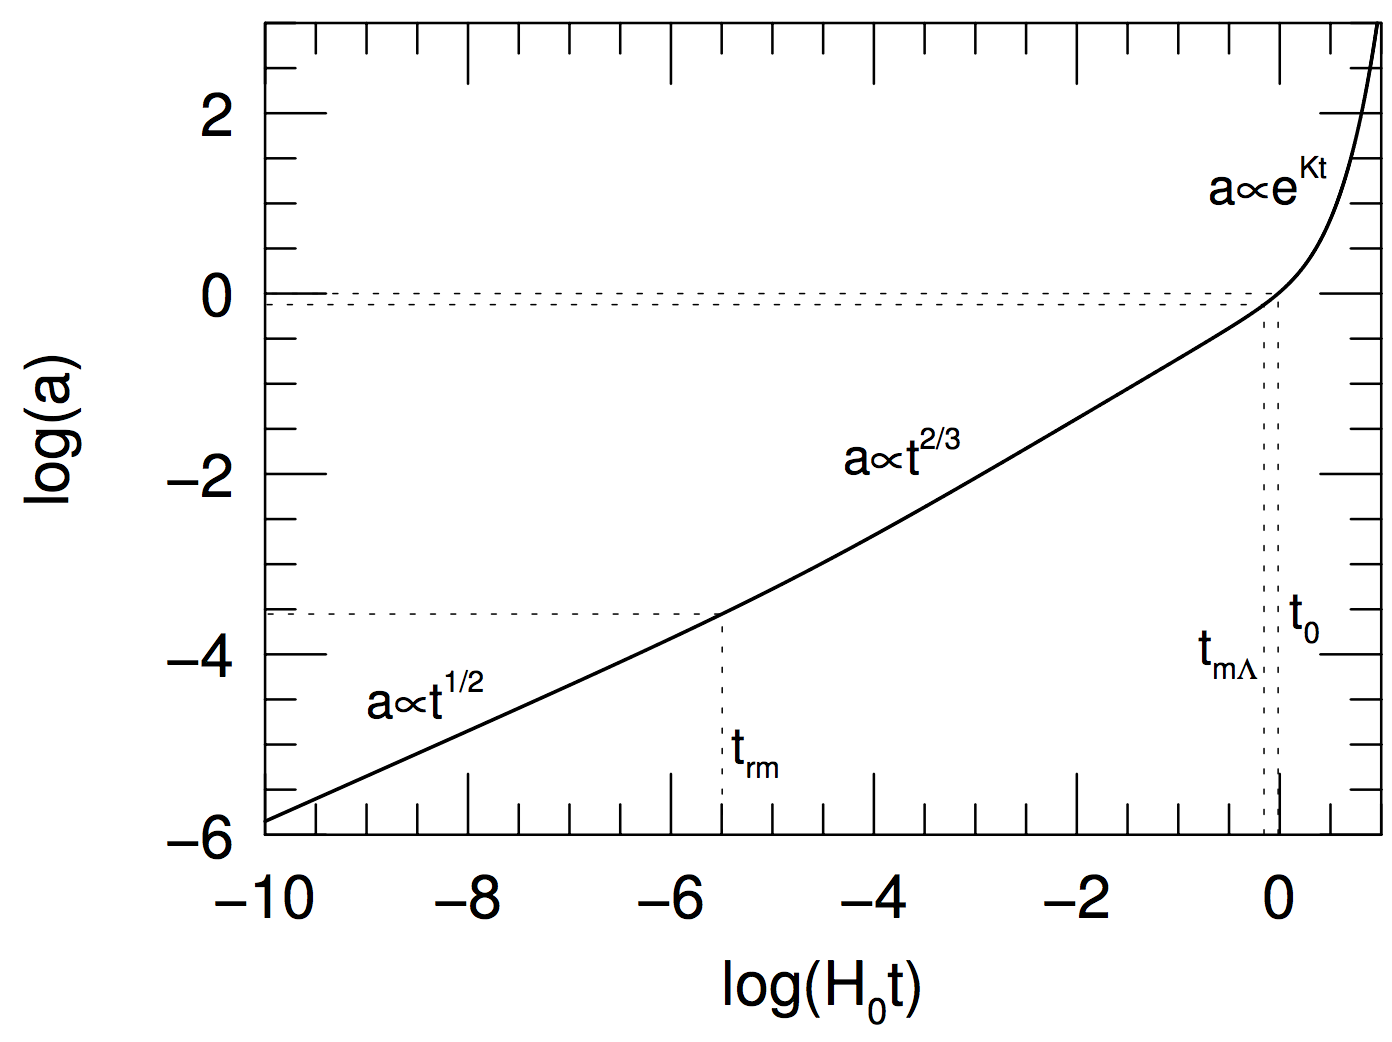
\includegraphics[width=12cm]{figures/avst.png}}
\end{figure}

{\noindent}The Hubble constant of the Benchmark Model is assumed to be $H_0=70\,{\rm km\,s^{-1}\,Mpc^{-1}}$. The radiation in the Benchmark Model consists of photons and neutrinos. The photons are assumed to be provided solely by a CMB with current temperature $T_0=2.725\,{\rm K}$ and density parameter $\Omega_{\gamma,0}=5.0\times10^{-5}$. The energy density of the CNB is theoretically calculated to be 68\% of that of the CMB, as long as neutrinos are relativistic. The matter content of the Benchmark Model consists partly of baryonic matter (that is, matter composed of protons and neutrons, with associated electrons), and partly of nonbaryonic dark matter. The evidence indicates that most of the matter in the universe is nonbaryonic dark matter. The baryonic material that we are familiar with from our everyday existence has a density parameter of $\Omega_{b,0}\approx0.04$ today. The density parameter of the nonbaryonic dark matter is roughly six times greater: $\Omega_{c,0}\approx0.26$. The bulk of the energy density in the Benchmark Model, however, is not provided by radiation or matter, but by a cosmological constant, with $\Omega_{\Lambda,0}=1-\Omega_{m,0}-\Omega_{r,0}\approx0.70$.

{\noindent}The Benchmark Model was first radiation-dominated, then matter-dominated, and is now entering into its lambda-dominated phase. Radiation gave way to matter at a scale factor $a_{rm}=\Omega{r,0}/\Omega{m,0}=2.8\times10^{-4}$, corresponding to a time $t_{rm}=4.7\times10^4\,{\rm yr}$. Matter, in turn, gave way to the cosmological constant at $a_{m\Lambda}=(\Omega_{m,0}/\Omega_{\Lambda,0})^{1/3}=0.75$, corresponding to $t_{m\Lambda}=9.8\,{\rm Gyr}$. The current age of the Universe, in the Benchmark Model, is $t_0=13.5\,{\rm Gyr}$.

{\noindent}With $\Omega_{r,0}$, $\Omega_{m,0}$ and $\Omega_{\Lambda,0}$ known, the scale factor $a(t)$ can be computed numerically using the Friedmann equation. Figure \ref{fig:avst} shows the scale factor, thus computed, for the Benchmark Model. Note that the transition from the $a\propto t^{1/2}$ radiation-dominated phase to the $a\propto t^{2/3}$ matter-dominated phase is not an abrupt one; neither is the later transition from the matter-dominated phase to the exponentially growing lambda-dominated phase. One curious feature of the Benchmark Model which Figure \ref{fig:avst} illustrates vividly is that we are living very close to the time of matter-lambda equality.


% --------------------------------------------------------------
%
%                           1. 
%
% --------------------------------------------------------------

\newpage
\subsection{Question 1}

What is recombination? At what temperature did it occur? Explain why this does not match the ionization potential of hydrogen.

\subsubsection{Short answer}

Recombination\footnote{A complete misnomer as the plasma has always been completely ionized up to this point} refers to the time at which the temperature of the early Universe became cool enough such that it was thermodynamically favourable for the ionized plasma of free electrons and ions to couple and form neutral atoms. Numerically, this might be defined as the moment when the number density of ions is equal to the number density of neutral atoms. This occurred at a temperature of $T \sim 1,000\,{\rm K}$ (corresponding to an energy of $\sim 0.1\,{\rm eV}$) at a redshift of $z \sim 1,100$. This does not match the ionization potential of hydrogen because the early Universe (as it was hot and dense) can be described by a blackbody with a characteristic distribution of photon energies including an exponential tail of high energy photons. While the peak of the blackbody spectrum describing the temperature of the early universe is below the ionization energy of hydrogen, the photons in the high-energy exponential tail of the blackbody spectrum have sufficient energies for ionization.

\subsubsection{Additional context}

The term \textit{re}combination is a common misnomer because this was in fact the first time that free electrons combined with ions to produce a neutral medium -- some cosmologists hold that ``combination'' would have been a more appropriate term. Prior to this time, the mean free path of the photons against scattering
off the free electrons is much less than the Hubble distance.
This means that gravitational forces attempting to compress the
plasma must also increase the photon density. This produces an
increase in temperature and hence in radiation pressure. Any perturbation in the baryon-photon plasma thus behaves as an acoustic
wave.

{\noindent}The ionization energy of hydrogen is $13.6\,{\rm eV}$. A photon $\gamma$ with an energy exceeding this ionization energy is capable of ionizing a hydrogen atom to produce a free electron $e$ and proton $p$ through the following process:

\begin{align*}
    {\rm H} + \gamma \rightarrow e + p.
\end{align*}

{\noindent}This process can of course run in reverse through the process of \textit{radiative recombination} where a free electron and proton can combine to produce a bound neutral hydrogen atom:

\begin{align*}
    e + p \rightarrow {\rm H} + \gamma.
\end{align*}

{\noindent}A crude approximation for the temperature at which recombination occurred could be made by assuming that the average photon energy must have been at least the ionization energy of hydrogen. Since the current temperature of the CMB is $2.7\,{\rm K}$, this should yield a lower limit on the recombination temperature:

\begin{align*}
    T_\mathrm{rec} \sim \frac{E_\mathrm{ion}}{E_\mathrm{CMB}} = \frac{13.6\,{\rm eV}}{k_B \cdot 2.7\,{\rm K}} \sim 60,000 ~ [{\rm K}].
\end{align*}

{\noindent}Clearly this is a very crude estimate since this is off by an order or magnitude, the recombination temperature being closer to $T \sim 1,000\,{\rm K}$. This is because this doesn't take into consideration the fact that the CMB photon energies are not single-valued as assumed above. When a dense, opaque object is in thermal equilibrium (such as the early Universe), the distribution of photon energies only depends on temperature following the blackbody function (or Planck function):

\begin{align}\label{eq:Planck}
    B_\nu(T) = \frac{2h\nu^3}{c^2} \frac{1}{\exp(h\nu/k_BT) - 1} ~ [{\rm erg\,s^{-1}\,cm^{-2}\,Hz^{-1}\,sr^{-1}}].
\end{align} 

\begin{figure}[h]
    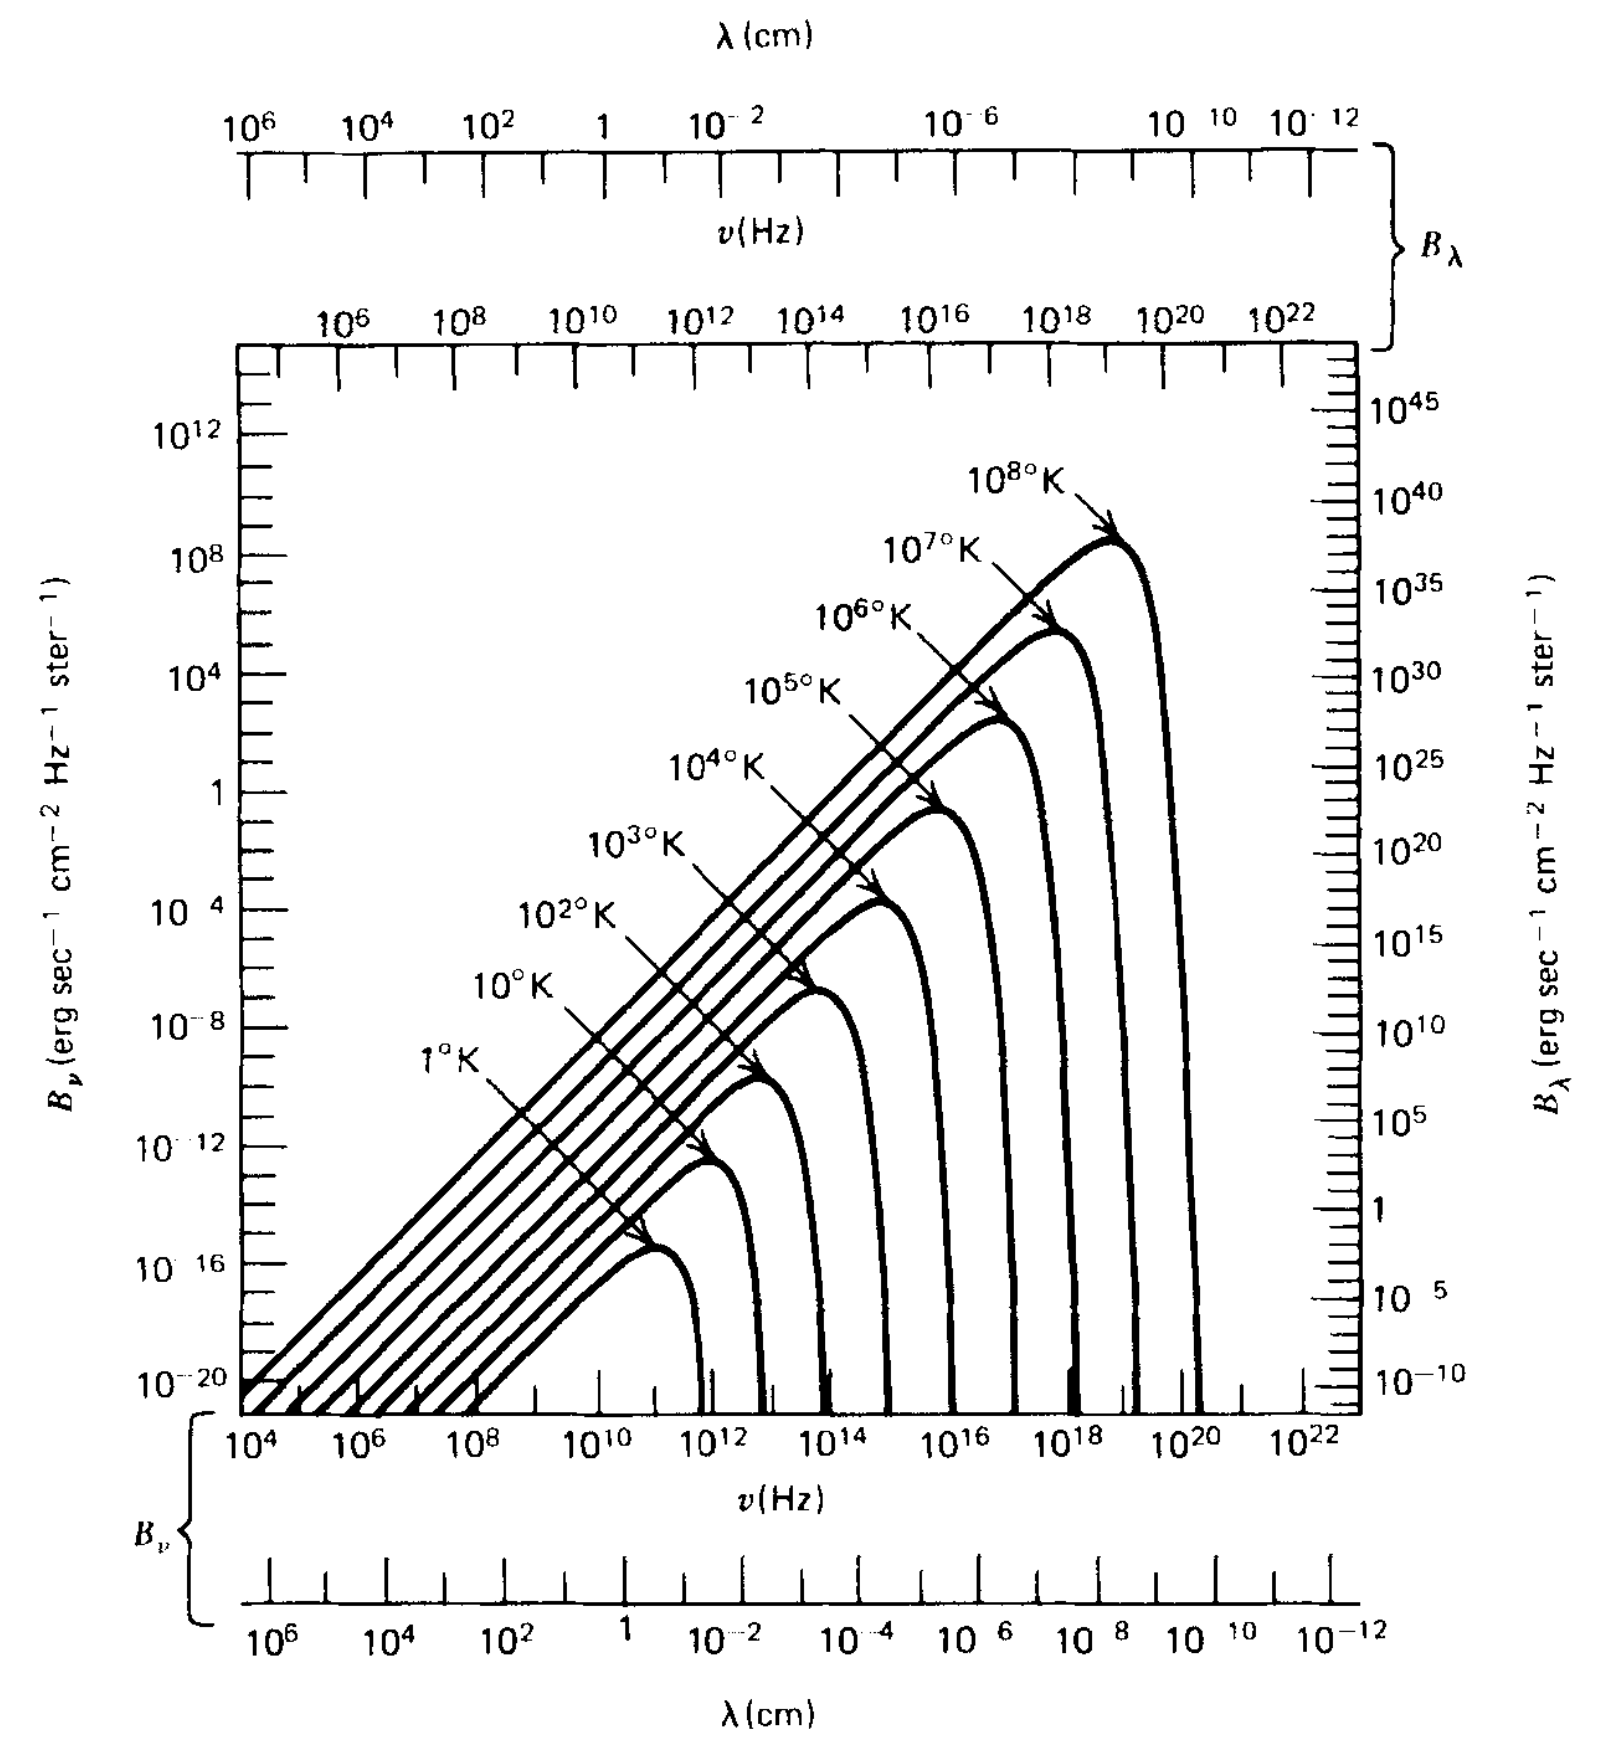
\includegraphics[width=14cm]{figures/blackbody.png}
    \centering
    \caption{Blackbody spectra at various temperatures. Figure taken from Ryden (2017).}
    \label{fig:blackbody}
\end{figure}

{\noindent}Figure \ref{fig:blackbody} shows blackbody spectra for various temperatures in log-log space, where the peak of each blackbody spectrum is related to its associated temperature via $h\nu_\mathrm{peak} \approx 2.82\,k_BT$. While the mean photon energy is $2.82\,k_BT$, approximately one in ever 500 photons will have energies exceeding $10\,k_BT$, one in 3 million will exceed $20\,k_BT$, and one in 30 billion will exceed $30\,k_BT$. While only a small fraction of CMB photons are found in the high-energy tail-end of the Planck distribution, the overall number of CMB photons is enormous -- outnumbering baryons by nearly 2 billion to one. Therefore, the vast number of CMB photons surrounding neutral hydrogen atoms greatly increases the probability of photoionization, even with a mean photon energy less than the ionization energy of hydrogen.

\begin{itemize}
    \item Before recombination, photon pressure is preventing collapse -- after recombination this photon pressure is suddenly gone and the Jeans mass drops by a factor of $\approx 10^{10}$ so structure starts growing again.
    \item By the end of recombination, silk damping has removed most of the small scale structure.
\end{itemize}

\subsubsection{Follow-up Questions}

\begin{itemize}
    \item How is the CMB related to recombination?
    \item Around how long ago or at what redshift did this occur?
\end{itemize}

% --------------------------------------------------------------
%
%                           2. 
%
% --------------------------------------------------------------

\newpage
\subsection{Question 2}

The universe is said to be ``flat," or, close to flat. What are the properties of a flat universe and what evidence do we have for it?

\subsubsection{Short answer}

There are three simple properties of a flat Universe: (1) parallel lines never converge nor diverge; (2) the sum of all energy densities is equal to it's critical value; and (3) the sum of angles withing a triangle is always $180^\circ$. Two common techniques for measuring the curvature (i.e., topology) of the Universe include measuring the total energy density of the Universe and using the main peak in the CMB power spectrum as a standard ruler.

\subsubsection{Additional context}

In developing a mathematical theory of general relativity, in which spacetime geometry/curvature is related to the mass-energy density, Einstein needed a way of mathematically describing curvature. Since picturing the curvature of a four-dimensional spacetime is, to say the least, difficult, let's start by considering ways of describing the curvature of two-dimensional spaces, then extend what we have learned to higher dimensions.

{\noindent}The simplest of two-dimensional spaces is a plane, on which Euclidean geometry holds (see (a) of Figure \ref{fig:geometries}). On a plane, a geodesic is a straight line. If a triangle is constructed on a plane by connecting three points with geodesics, the sum of the angles made with its vertices obeys:

\begin{align*}
    \Delta_\mathrm{flat} = \alpha + \beta + \gamma = \pi ~~~~~[{\rm rad}].
\end{align*}

{\noindent}Note that a plane has infinite area, and has no upper limits on the possible distance between points.

{\noindent}Now consider another simple two-dimensional space, the surface of a sphere (see (b) of Figure \ref{fig:geometries}). On the surface of a sphere, a geodesic is a portion of a great circle -- that is, a circle whose center corresponds to the center of the sphere. If a triangle is constructed on the surface of the sphere by connecting three points with geodesics, the sum of the angles made with its vertices obeys:

\begin{align*}
    \Delta_\mathrm{closed} = \alpha + \beta + \gamma = \pi + A/R^2 ~~~~~[{\rm rad}],
\end{align*}

{\noindent}where $A$ is the area of the triangle, and $R$ is the radius of the sphere. All spaces in which $\alpha + \beta + \gamma > \pi$ are called ``positively curved'' spaces. The surface of a sphere is a positively curved two-dimensional space. Moreover, it is a space where the curvature is homogeneous and isotropic; no matter where you draw a triangle on the surface of a sphere, or how you orient it, it must always satisfy the above equation for $\Delta_\mathrm{closed}$. Note that a sphere has a maximum possible distance between points; the distance between antipodal points, at the maximum possible separation, is $\pi R$.

{\noindent}In addition to flat spaces and positively curved spaces, there exist negatively curved spaces. An example of a negatively curved two-dimensional space is the hyperboloid, or saddle-shape (see (c) of Figure \ref{fig:geometries}). If a triangle is constructed on this surface by connecting three points with geodesics, the sum of the angles made with its vertices obeys:

\begin{align*}
    \Delta_\mathrm{open} = \alpha + \beta + \gamma = \pi - A/R^2 ~~~~~[{\rm rad}],
\end{align*}

{\noindent}where $A$ is the area of the triangle, and $R$ is the radius of curvature. All spaces in which $\alpha + \beta + \gamma < \pi$ are called ``negatively curved'' spaces. The surface of a hyperboloid is a negatively curved two-dimensional space. A surface of constant negative curvature has infinite area, and has no upper limit on the possible distance between points.

\begin{figure}[h]
    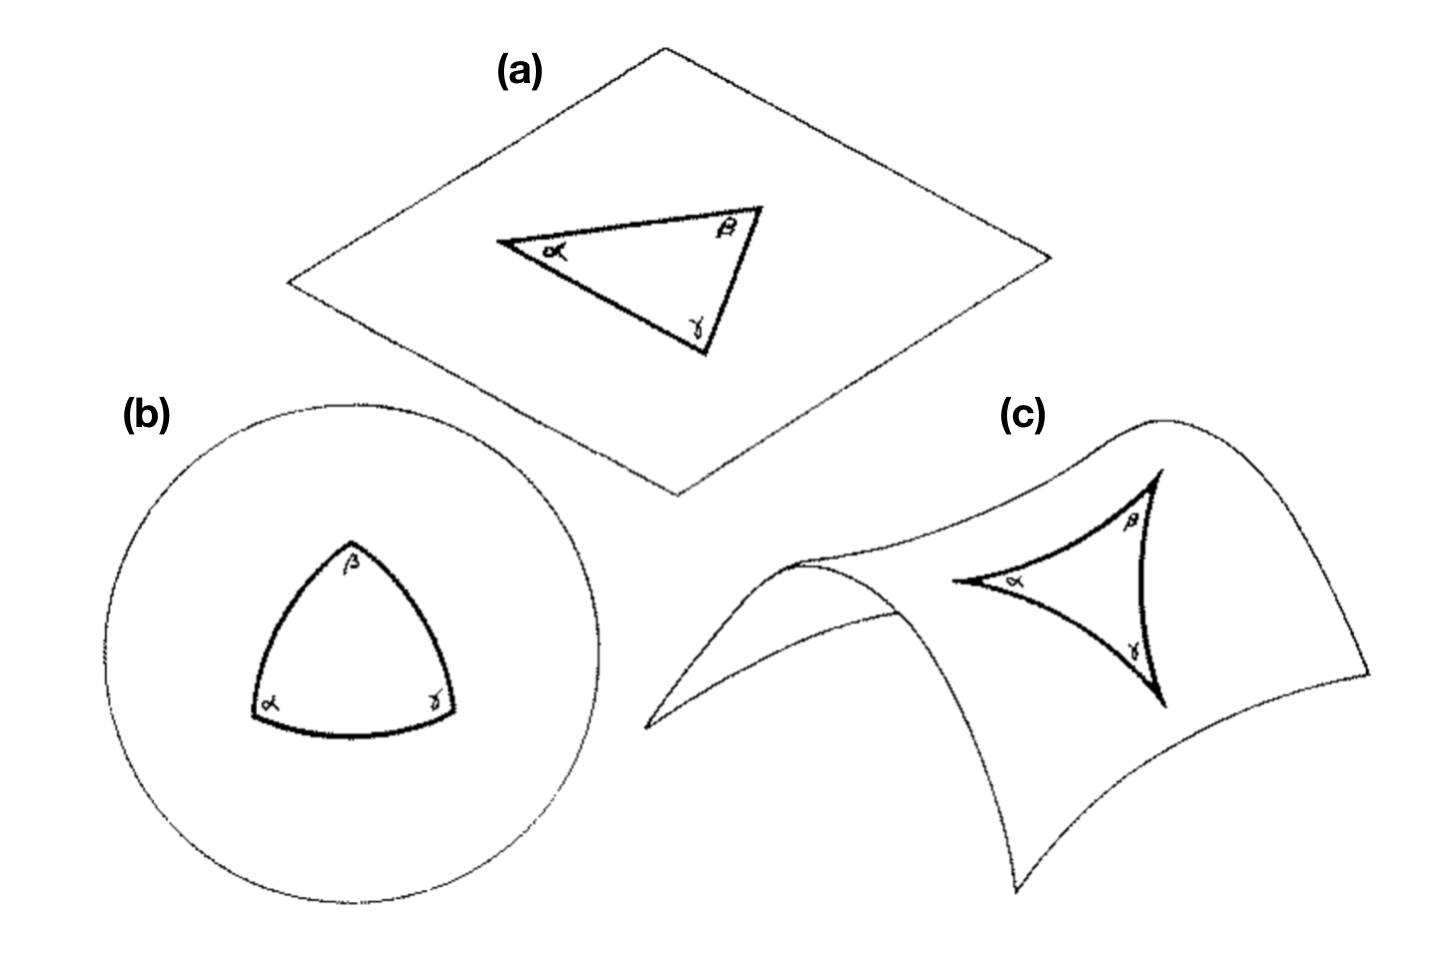
\includegraphics[width=14cm]{figures/geometries.png}
    \centering
    \caption{(a) Flat geometry for which $ \Delta_\mathrm{flat} = \alpha + \beta + \gamma = \pi$. (b) Closed geometry for which $\Delta_\mathrm{closed} = \alpha + \beta + \gamma = \pi + A/R^2$, where $A$ is the area of the triangle, and $R$ is the radius of the sphere. (c) Open geometry for which $\Delta_\mathrm{open} = \alpha + \beta + \gamma = \pi - A/R^2$, where $A$ is the area of the triangle, and $R$ is the radius of curvature.}
    \label{fig:geometries}
\end{figure}

{\noindent}If you want a two-dimensional space to be homogeneous and isotropic, there are only three possibilities that fit the bill: the space can be uniformly flat, it can have uniform positive curvature, or it can have uniform negative curvature. Thus, if a two-dimensional space has curvature which is homogeneous and isotropic, its geometry can be specified by two quantities, $\kappa$, and $R$. The number $\kappa$, called the curvature constant, is $\kappa = 0$ for a flat space, $\kappa = +1$ for a positively curved space, and $\kappa = −1$ for a negatively curved space. If the space is curved, then the quantity $R$, which has dimensions of length, is the radius of curvature.

{\noindent}The results for two-dimensional space can be extended straightforwardly to three dimensions. A three-dimensional space, if its curvature is homogeneous and isotropic, must be flat, have uniform positive curvature, or have uniform negative curvature. If a three-dimensional space is flat ($\kappa = 0$), it has the following metric:

\begin{align*}
    ds^2_\mathrm{flat} = dx^2 + dy^2 + dz^2.
\end{align*}

{\noindent}By making the simple coordinate substitution $x = r\cos\theta$, $y = r\sin\theta$, this can be written in spherical coordinates as:

\begin{align*}
    ds^2_\mathrm{flat} = dr^2 + r^2[d\theta^2 + \sin^2\theta d\phi^2].
\end{align*}

{\noindent}If a three-dimensional space has uniform positive curvature ($\kappa = +1$), its metric is

\begin{align*}
    ds_\mathrm{closed}^2 = dr^2 + R^2\sin^2(r/R)[d\theta^2 + \sin^2\theta d\phi^2].
\end{align*}

{\noindent}A positively curved three-dimensional space has finite volume, just as a positively curved two-dimensional space has finite area. The point at $r = \pi R$ is the antipodal point to the origin, just as the south pole, at $r = \pi R$, is the antipodal point to the north pole, at $r = 0$, on the surface of a sphere. By traveling a distance $C = 2\pi R$, it is possible to ``circumnavigate'' a space of uniform positive curvature.

{\noindent}If a three-dimensional space has uniform negative curvature ($\kappa =
−1$), its metric is

\begin{align*}
    ds_\mathrm{open}^2 = dr^2 + R^2\sinh^2(r/R)[d\theta^2 + \sin^2\theta d\phi^2].
\end{align*}

{\noindent}Like flat space, negatively curved space has infinite volume.

{\noindent}The three possible metrics for a homogeneous, isotropic, three-dimensional
space can be written more compactly in the form:

\begin{align*}
    ds^2 = dr^2 + S_\kappa(r)^2d\Omega^2
\end{align*}

{\noindent}where

\begin{align*}
    d\Omega \equiv d\theta^2 + \sin^2\theta d\phi^2
\end{align*}

{\noindent}and

\begin{equation*}
    S_\kappa(r) =
    \left\{
    \begin{aligned}
    R\sin(r/R), ~~~~~& (\kappa = +1) \\
              r,~~~~~& (\kappa = 0) \\
    R\sinh(r/R),~~~~~& (\kappa = -1)
    \end{aligned}
    \right.
    .
\end{equation*}

{\noindent}The coordinate system ($r,\theta,\phi$) is not the only possible system. For instance, if we switch the radial coordinate from $r$ to $x \equiv S_\kappa(r)$, the metric for a homogeneous, isotropic, three-dimensional space can be written in the form:

\begin{align*}
    ds^2 = \frac{dx^2}{1-\kappa x^2/R^2} + x^2d\Omega^2.
\end{align*}

The \textbf{critical density} of the Universe is defined to be

\begin{align*}
    \rho_c \equiv \left( \frac{3H_0}{8\pi G} \right) ~ [{\rm g\,cm^{-3}}].
\end{align*}

{\noindent}If the total energy density is higher than this, then the Universe is said to be \textbf{closed}: initially parallel lines eventually converge, just as lines of constant longitude meet at the North and South poles. A closed Universe, much like the surface of a sphere, has positive curvature. In a low-density Universe whose total energy density is less than critical value, the Universe is said to be \textbf{open}: initially parallel lines eventually diverge, as would marbles rolling off a saddle. While a closed Universe has positive curvature, an open Universe has negative curvature.

% --------------------------------------------------------------
%
%                           3. 
%
% --------------------------------------------------------------

\newpage
\subsection{Question 3}

Outline the development of the Cold Dark Matter spectrum of density fluctuations from the early universe to the current epoch.

\subsubsection{Short answer}

Answer.

\subsubsection{Additional context}

The generally accepted theoretical framework for the formation of structure is that of gravitational instability. The gravitational instability scenario assumes that the early universe was almost perfectly smooth, with the exception of tiny density perturbations with respect to the global cosmic background density and the accompanying tiny velocity perturbations from the general Hubble expansion. The observed fluctuations in the CMB temperature are a reflection of these density perturbations, so we know that the primordial density perturbations must have been on the order of $\Delta T / T \sim 10^{-5}$. The origin of this density perturbation field has yet to be fully understood, but the most plausible theory currently is that they are a result of \textit{quantum fluctuations} which, during the inflationary phase, expanded to macroscopic scales.

{\noindent}Originally minute deviations from the average density of the Universe, and the corresponding deviations from the global cosmic expansion velocity (i.e., the Hubble expansion), will start to grow under the influence of gravity where the density perturbations will have induced local differences in gravity. During its early evolution, an overdensity will experience a gradually stronger deceleration of its expansion velocity such that its expansion velocity will continue to slow down with respect to the Hubble expansion. Since matter is gravitationally attracted to regions of higher density, it will also have the tendency to move towards that region. When the region has become sufficiently overdense, the mass of the density perturbation will have grown so much that its expansion would come to a halt. The region then completely decouples from the Hubble expansion and begins to collapse under its own gravity. The newly formed gravitationally bound object will reach virial equilibrium at which point it becomes a recognizable comic object; its precise nature (e.g., galaxy, cluster etc.) being determined by the properties of the initial density perturbation and its surroundings.

{\noindent}The opposite tendency will have occurred for underdensities in the matter density field. Since they contain less matter than the average density field, its expansion deceleration is less than the Hubble expansion which results in matter becoming even more dispersed and underdensities continuing to expand. As this process continues and becomes more pronounced, such underdensities result in the gradual emergence of voids in the matter distribution of the Universe. The most dramatic evidence for these spatial nonuniformities (i.e., overdensities and voids) on the largest of scales comes from redshift surveys such as the 2dF Galactic Redshift Survey\footnote{\href{http://www.2dfgrs.net/}{2dFGRS: http://www.2dfgrs.net/}} shown in Figure \ref{fig:2df}.

\begin{figure}[h]
    \floatbox[{\capbeside\thisfloatsetup{capbesideposition={right,top},capbesidewidth=4cm}}]{figure}[\FBwidth]
    {\caption{\footnotesize{The spatial distribution of galaxies in two four-degree strips on the sky, according to the 2dF Galaxy Redshift Survey. Note the $100\,{\rm Mpc}$ filamentary features and the prominent voids. One of the principal challenges in cosmology is to explain this pattern, which is most probably a relic of the very earliest stages of the expanding Universe. Figure taken from Ryden (2017).}}
    \label{fig:2df}}
    {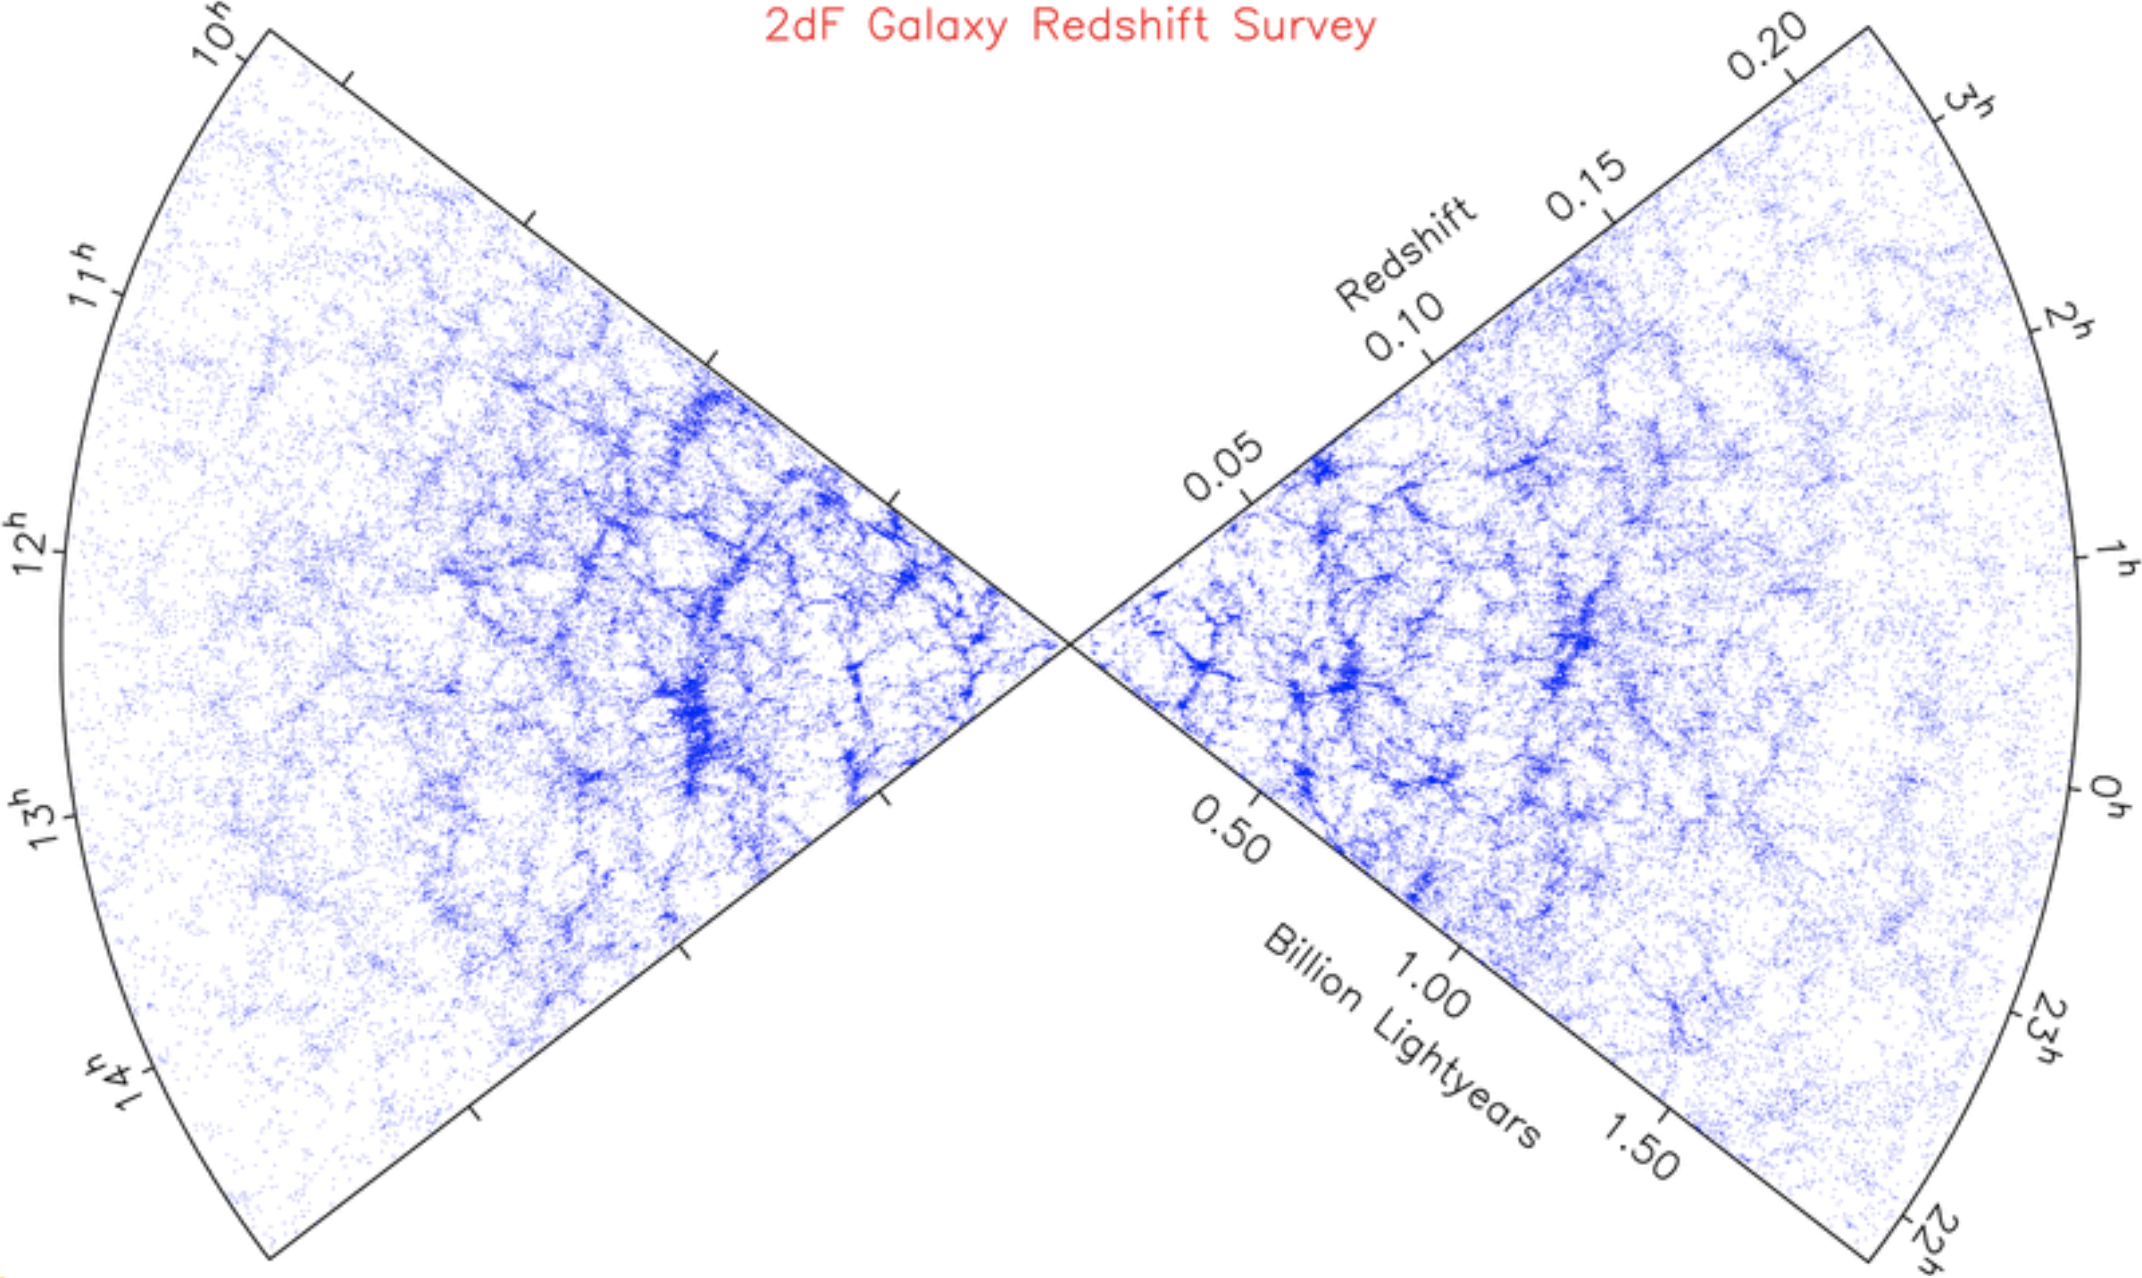
\includegraphics[width=10cm]{figures/2df.png}}
\end{figure}

{\noindent}Galaxies in Figure \ref{fig:2df} are clearly not distributed randomly: the Universe has structure on large scales. To understand this structure, we must go beyond the Standard Model not only by including dark matter, but also by allowing for deviations from smoothness. We must develop the tools to study perturbations around the smooth background of the Standard Model. This is straightforward in theory, as long as the perturbations remain small (i.e., linear). Indeed, understanding the development of structure in the universe has become a major goal of most cosmologists today. Dark matter is needed not only to explain rotation curves of galaxies but to explain structure in the Universe at large!

{\noindent}The best ways to learn about the evolution of structure and to compare theory with observations are to look at anisotropies in the CMB and at how matter is distributed on large scales. Anisotropies in the CMB today tell us what the Universe looked like when it was several hundred thousand years old, so they are wonderful probes of the perturbations. To compare theory with observations, we must at first try to avoid scales dominated by nonlinearities. As an extreme example, we can never hope to understand cosmology by carefully examining rock formations on Earth. The intermediate steps -- collapse of matter into a galaxy; molecular cooling; star formation; planetary formation; etc. -- are much too complicated to allow comparison between linear theory and observations. While perturbations to matter on small scales (less than about $100\,{\rm Mpc}$) have grown nonlinear, large-scale perturbations are still small so they have been processed much less than the corresponding small-scale structure. Similarly, anisotropies in the CMB have remained small because the photons that make up the CMB do not clump.

{\noindent}Identifying large-scale structure and the CMB as the two most promising areas of study solves just one issue. Another very important challenge is to understand how to characterize these distributions so that theory can be compared to experiment. It is one thing to look at a map and quite another to quantitatively test cosmological models. To make such tests, it is often useful to take the Fourier transform of the distribution in question; as we will see, working in Fourier space makes it easier to separate large from small scales. The most important statistic in the cases of both the CMB and large-scale structure is the \textbf{two-point correlation function}, called the \textbf{power spectrum} in Fourier space.

{\noindent}If the mean density of galaxies at some time $t$ is $\langle\rho(t)\rangle$, then we can characterize the inhomogeneities with the dimensionless \textbf{density perturbation field} (also known as the \textbf{density contrast}) which is used to relate the energy density $\rho(\mathbf{x},t)$ at some co-moving spatial coordinate $\mathbf{x}$ and time $t$ to the average energy density at that time $\langle\rho(t)\rangle$:

\begin{align*}
    \delta(\mathbf{x},t) \equiv \frac{\rho(\mathbf{x},t)~- \langle\rho(t)\rangle}{\langle\rho(t)\rangle} ~ [{\rm dimensionless}].
\end{align*}

{\noindent}Evidently, in an unperturbed Universe with $\rho(\mathbf{x},t) = \langle\rho(t)\rangle$ everywhere, $\delta(\mathbf{x},t) = 0$. Note that positive density fluctuations (i.e., overdensities) may in principle grow limitless whereas negative density fluctuations (i.e., underdensities) have a strict lower-limit of $\delta \geq -1$ (emptier than empty simply doesn't exist). In a complete description of density perturbations, the total energy density of the Universe includes components of baryonic matter ($\rho_b$), cold dark matter ($\rho_c$), radiation ($\rho_\mathrm{rad}$), and dark energy ($\rho_\Lambda$):

\begin{align*}
    \rho(\mathbf{x},t) = \rho_b(\mathbf{x},t) + \rho_c(\mathbf{x},t) + \rho_\mathrm{rad}(\mathbf{x},t) + \rho_\Lambda(\mathbf{x},t) ~ [{\rm g\,cm^{-3}}].
\end{align*}

{\noindent}In terms of their global gravitational influence, dark matter and baryonic matter contribute and evolve equivalently, therefore on cosmological scales they can be combined into a total matter energy density $\rho_m = \rho_b + \rho_c$. Each component may have its own (primordial) perturbation character. Dark energy does not have any density fluctuations, so $\delta_\Lambda(\mathbf{x},t) = 0$. Since most of the structure formation happened during the \textit{matter-dominated era}, this mainly involves the evolution of matter linear perturbations $\delta_m(\mathbf{x},t)$.

{\noindent}In addition to the density contrast, an alternative (and equivalent) description of the statistical properties of the matter distribution in the Universe is the \textbf{power spectrum} $P(k)$. Roughly speaking, the power spectrum describes the level of structure as a function of the length scale $L \simeq 2\pi/k$ where $k$ is a co-moving wavenumber. Phrased differently, the density fluctuations are decomposed into a set of plane waves of the form $\delta(\mathbf{x}) = \sum a_k\cos(\mathbf{x\cdot k})$ with wave vector $\mathbf{k}$ and amplitude $a_k$. The power spectrum $P(k)$ then describes the mean of the squares of the amplitudes $\lvert a_k \rvert^2$ averaged over all wave vectors with equal length $\lvert\mathbf{k}\rvert = k$. Technically speaking, this is a Fourier decomposition. The Fourier transform of $\delta(\mathbf{x},t)$ is $\tilde{\delta}(\mathbf{x},t)$, which allows the power spectrum $P(k)$ to be defined via

\begin{align*}
    \langle \tilde{\delta}(\mathbf{k}) \tilde{\delta}(\mathbf{k'}) \rangle = (2\pi)^3 P(k) \delta^3 (\mathbf{k} - \mathbf{k'}),
\end{align*}

{\noindent}where the angular brackets denote averaging over the entire distribution, $k$ is the wavenumber, and $\delta^3()$ is the delta Dirac function which constrains $\mathbf{k}=\mathbf{k'}$. This indicates that the power spectrum is the spread, or the variance, in the distribution. Figure \ref{fig:galaxypowerspec} shows the combination $k^3P(k)/2\pi^2$, a dimensionless number which is a good indication of the clumpiness on scale $k$.

{\noindent}The power spectrum $P(k)$ and the two-point correlation function $\xi(x)$ are related through the Fourier transform as

\begin{align*}
    P(k) = 2\pi \int\limits_0^\infty \frac{\sin(kx)}{kx} x^2 \xi(x)\,{\rm d}x,
\end{align*}

{\noindent}i.e., the integral over the correlation function with a weight factor depending on the wave number provides the power spectrum. This relation can also be inverted to obtain the inverse Fourier transform such that the correlation function can be computed from the power spectrum. In general, knowing the power spectrum is insufficient to unambiguously describe the statistical properties of any density field; as such, the power spectrum is often used alongside the correlation function $\xi(x)$. Given observation data, either the power spectrum or the correlation function may be easier to compute, or another may be easier to obtain from models or simulations. In addition, our intuitive understanding of these functions may vary in different situations.

\begin{figure}[t]
    \floatbox[{\capbeside\thisfloatsetup{capbesideposition={right,top},capbesidewidth=4cm}}]{figure}[\FBwidth]
    {\caption{\footnotesize{The variance $\Delta^2 \equiv k^3P(k)/2\pi^2$ of the Fourier transform of the galaxy distribution as a function of scale. On large scales, the variance is smaller than unity so the distribution is smooth. The solid line is the theoretical model in which the Universe contains dark matter and a cosmological constant with perturbations generated by inflation. The dashed line is a model with only baryons and no dark matter. Data came from the PSCz survey (Saunders et ai, 2000) as analyzed by Hamilton and Tegmark (2001). Figure from Ryden (2017).}}
    \label{fig:galaxypowerspec}}
    {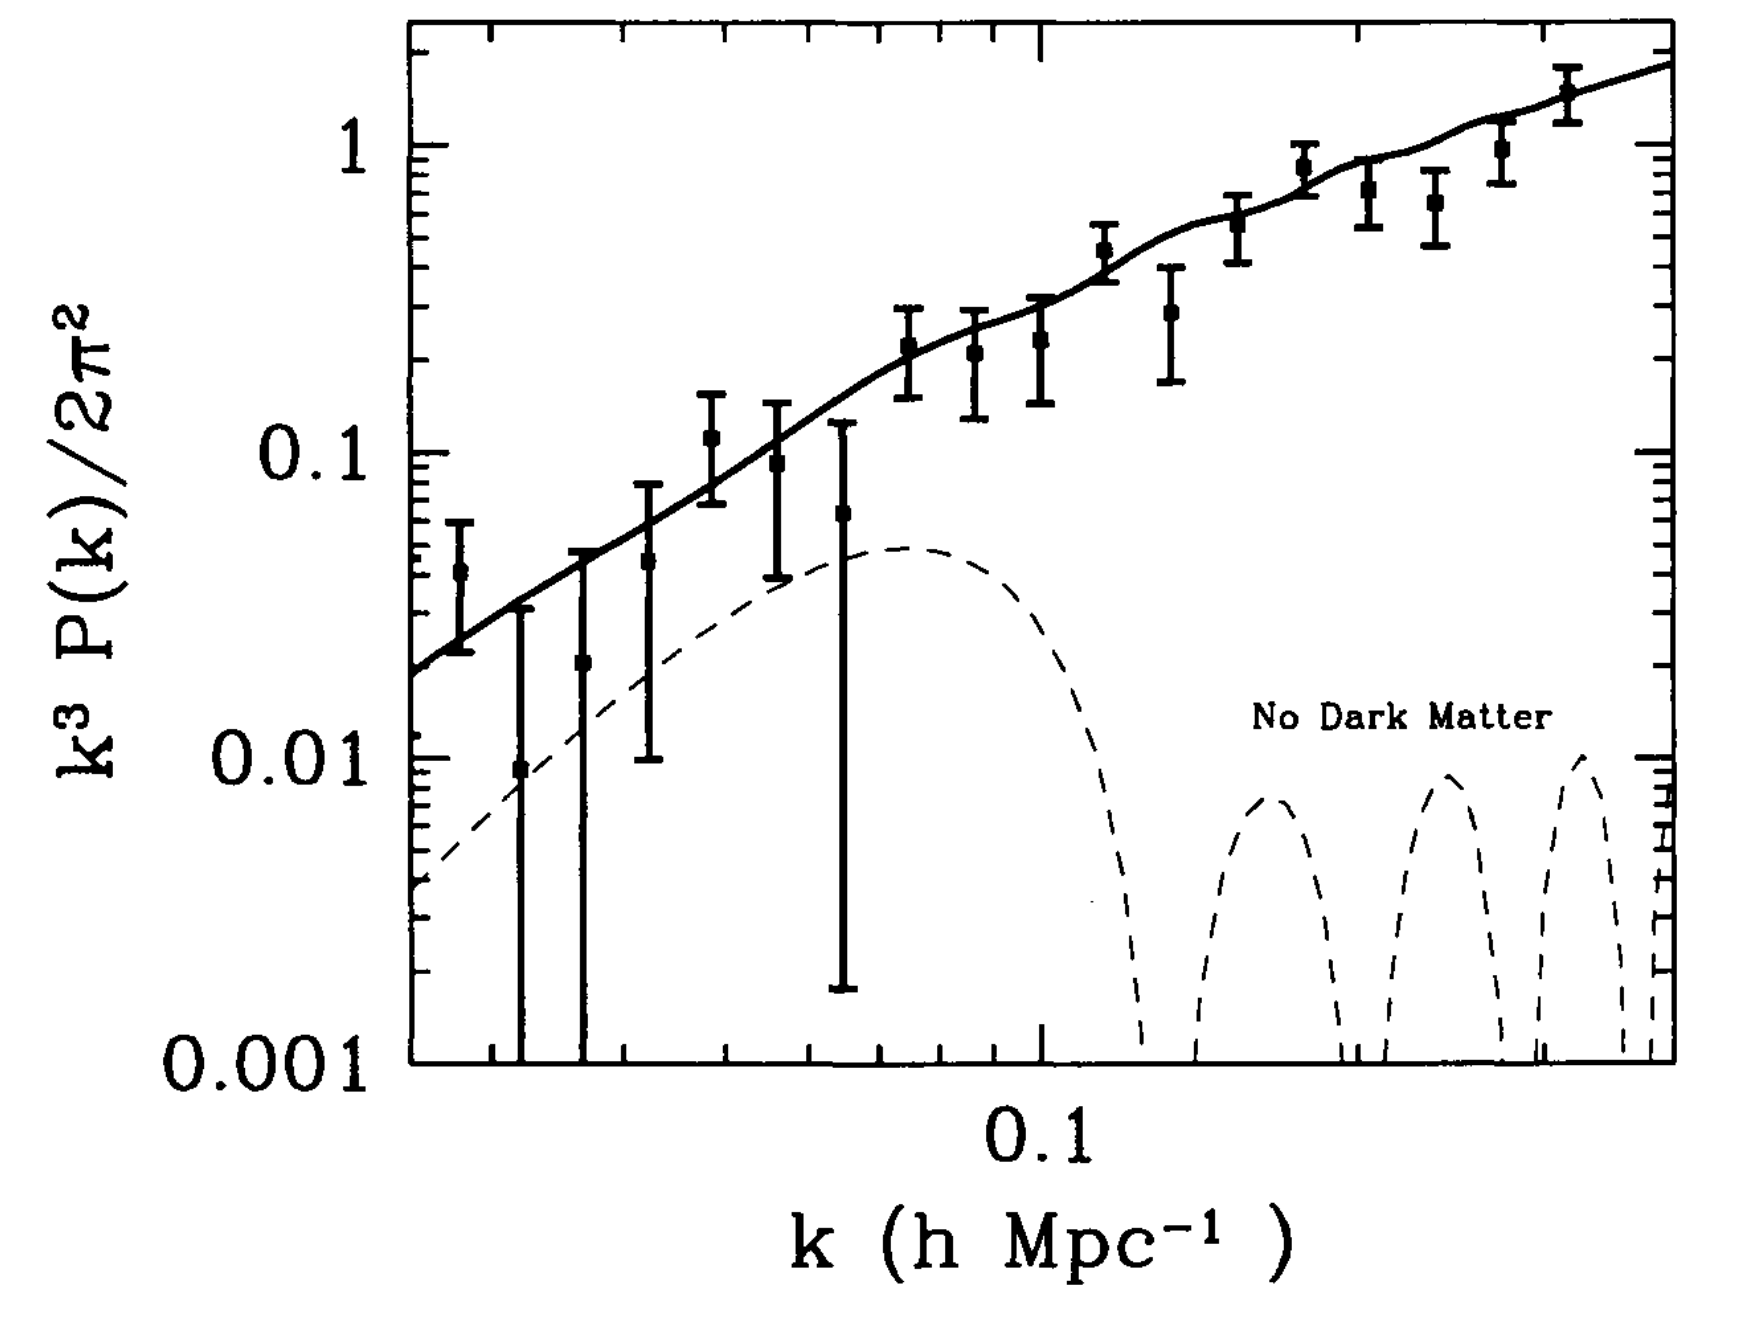
\includegraphics[width=12cm]{figures/GalaxyPowerSpectrum.png}}
\end{figure}

\begin{figure}[h]
    \floatbox[{\capbeside\thisfloatsetup{capbesideposition={right,top},capbesidewidth=4cm}}]{figure}[\FBwidth]
    {\caption{\footnotesize{Anisotropies in the CMB predicted by the theory of inflation compared with observations, x-axis is multipole moment (e.g., $\ell = 1$ is the dipole, $\ell = 2$ the quadrupole) so that large angular scales correspond to low $\ell$; y-axis is the root mean square anisotropy (the square root of the two-point correlation function) as a function of scale. The characteristic signature of inflation is the series of peaks and troughs, a signature which has been verified by experiment. Figure from Ryden (2017).}}
    \label{fig:cmbpowerspec}}
    {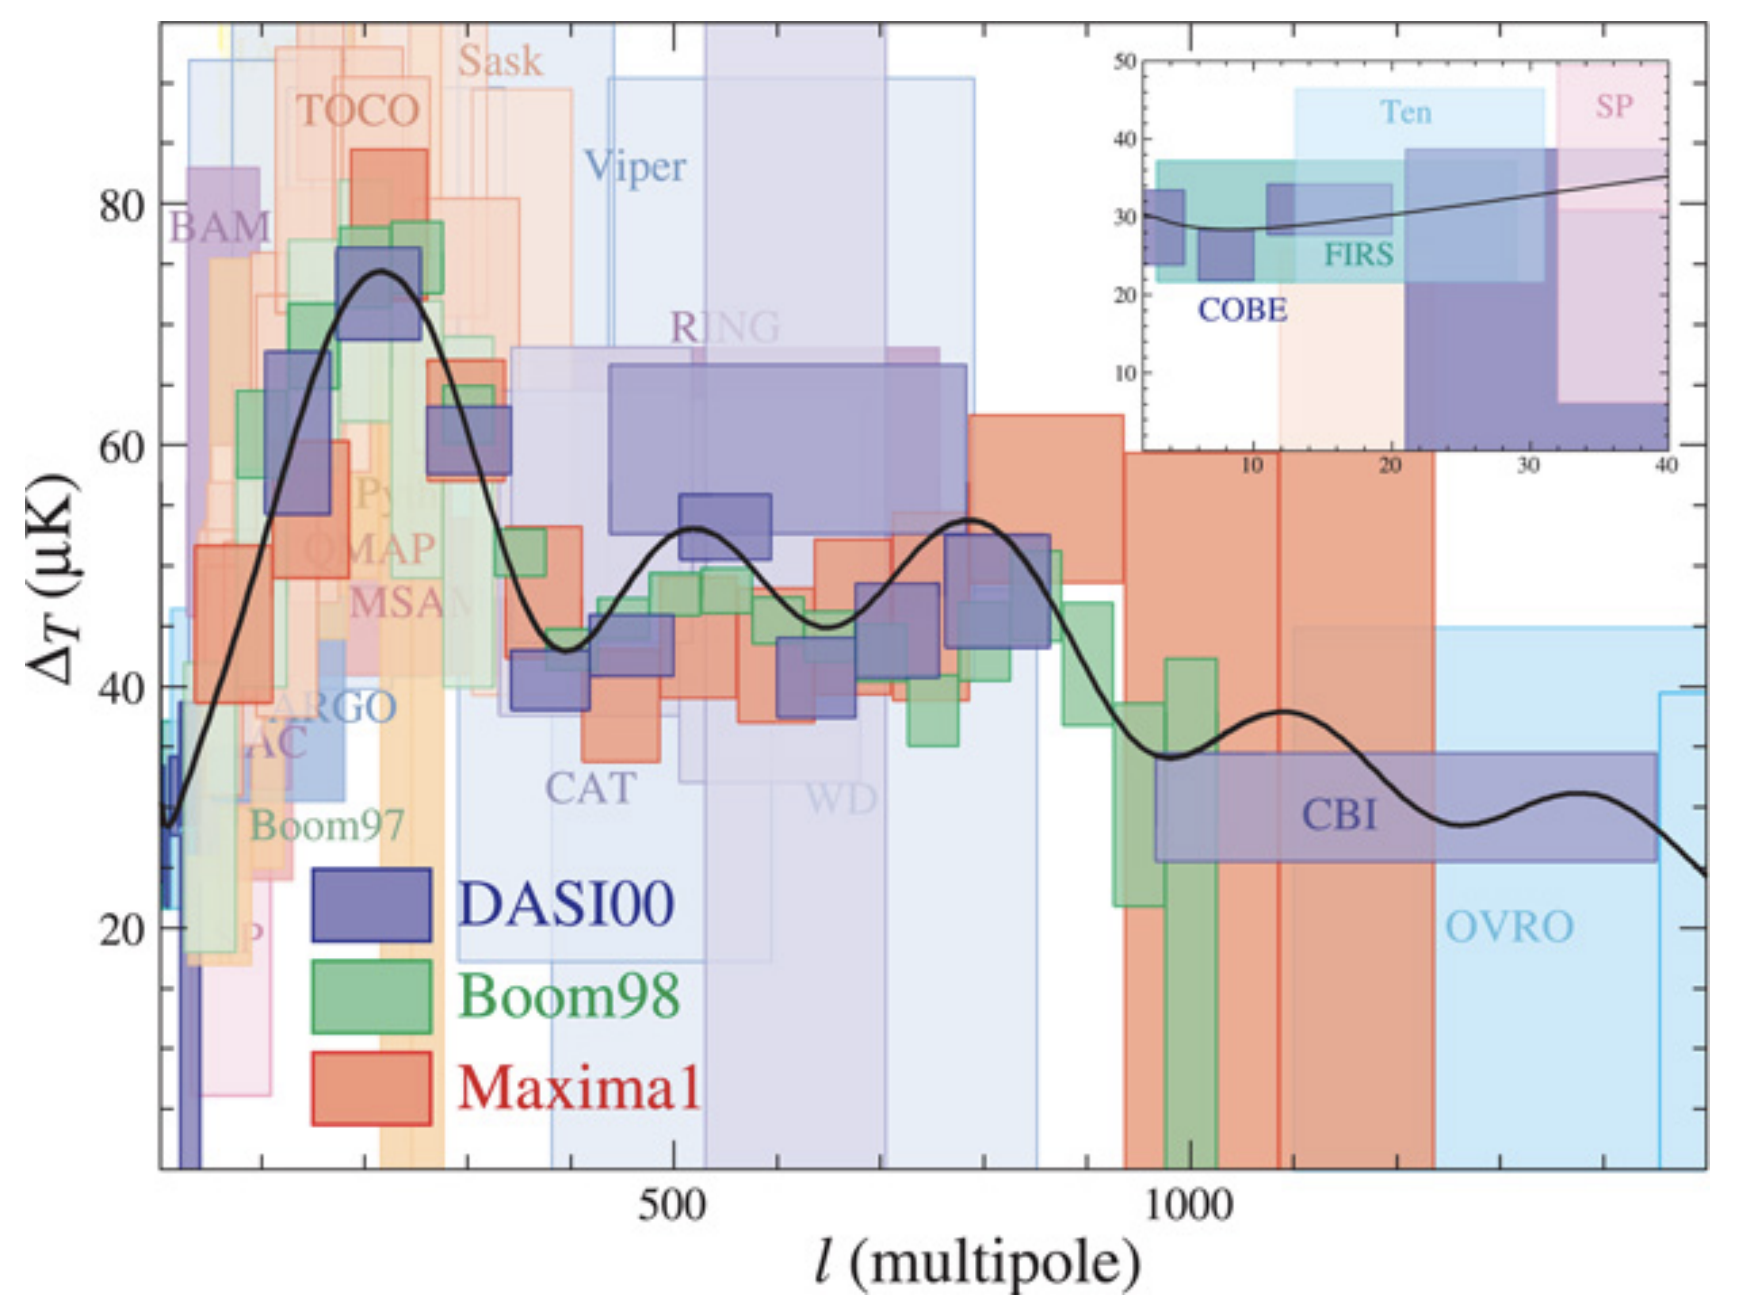
\includegraphics[width=12cm]{figures/CMBPowerSpectrum.png}}
\end{figure}

{\noindent}The best measure of anisotropies in the CMB is also the two-point correlation function of the temperature distribution. There is a subtle technical difference between the two power spectra which are used to measure the galaxy distribution and the CMB, though. The difference arises because the CMB temperature is a two-dimensional field, measured everywhere on the sky (i.e., with two angular coordinates). Instead of Fourier transforming the CMB temperature, then, one typically expands it in spherical harmonics, a basis more appropriate for a 2D field on the surface of a sphere. Therefore the two-point correlation function of the CMB is a function of multipole moment $\ell$, not wave number $k$. Figure \ref{fig:cmbpowerspec} shows the measurements of dozens of groups since 1992, when COBE first discovered large-angle (low $\ell$ in the plot) anisotropies.

{\noindent}It is assumed that in very early epochs, the matter density field obeyed Gaussian statistics. This is a prediction of a large class of inflationary models which are supposed to generate the primordial density fluctuations of the Universe. An important property of Gaussian statistics, or \textit{Gaussian random fields}, is that their distributions are uniquely determined by their power spectrum $P(k)$. Among the properties which characterize these Gaussian random fields, the probability distribution of the density fluctuations $\delta(\mathbf{x})$ at any point is a Gaussian distribution. Observational evidence for the Gaussian nature of the early density fluctuations comes from observations of anisotropies in the CMB which very strongly constrain any possible deviation from a Gaussian random field in the early Universe.

{\noindent}The early linear stages of structure formation have been successfully and completely worked out within the context of \textit{linear perturbation theory}. For this discussion of the growth of density perturbations, we are concentrating on length scales that are substantially smaller than the Hubble radius. On such scales, structure growth can be described in the framework of the Newtonian theory of gravity; the effects of spacetime curvature and thus General Relativity need only be accounted for when density perturbations are on length scales comparable to, or larger than, the Hubble radius. In addition, we assume for simplicity that the matter in the Universe consists of only pressure-free matter described in the \textit{fluid approximation}.

{\noindent}Approximate solutions of the set of equations which describe small deviations from the homogeneous solution have the form

\begin{align*}
    \delta(\mathbf{x},t)=D(t)\tilde{\delta}(\mathbf{x}),
\end{align*}

{\noindent}i.e., the spatial and temporal dependencies factorize in these solutions. Here, $\tilde{\delta}(\mathbf{x})$ is an arbitrary function of the spatial coordinate, and D(t) satisfies the equation

\begin{align*}
    \ddot{D}(t)+\frac{2\dot{a}}{a}\dot{D}(t)-4\pi G\bar{\rho}(t)D(t) = 0.
\end{align*}

{\noindent}The differential equation has two linearly independent solutions. One can show that one of them increases with time, whereas the other decreases. If, at some early time, both functional dependencies were present, the increasing solution will dominate at later times, whereas the solution decreasing with $t$ will become irrelevant. Therefore, we will consider only the increasing solution, which is denoted by $D_+(t)$, and normalize it such that $D_+(t_0)=1$. Then, the density contrast becomes

\begin{align*}
    \delta(\mathbf{x},t) = D_+(t)\delta_0(\mathbf{x}).
\end{align*}

{\noindent}This mathematical consideration allows us to draw immediately a number of conclusions. First, the solution implies that in linear perturbation theory the spatial shape of the density fluctuations is frozen in comoving coordinates, only their amplitude increases. The growth factor $D_+(t)$ of the amplitude follows a simple differential equation that is readily solvable for any cosmological model. In fact, one can show that for arbitrary values of the density parameters in matter and vacuum energy, the growth factor has the form

\begin{align*}
    D_+(t) \propto \frac{H(a)}{H_0}\int\limits_0^a \frac{da'}{[\Omega_m/a'+\Omega_\Lambda a'^2-(\Omega_m+\Omega_\Lambda-1)]^{3/2}},
\end{align*}

{\noindent}where the factor of proportionality is determined from the condition $D_+(t_0)=1$.

{\noindent}Primordial density perturbations on a small scale appear to have a much higher amplitude than those on larger scales. This leads to a hierarchical process of structure formation, with small-scale perturbations being the first one to become nonlinear and develop into cosmic objects.

{\noindent}Returning to the two-point correlation function and Fourier transform, $P(k)$ and $\xi(x)$ both depend on cosmological time or redshift because the density field in the Universe evolves over time. Therefore, the dependence on $t$ is explicitly written as $P(k,t)$ and $\xi(x,t)$. Note that $P(k,t)$ is linearly related to $\xi(x,t)$ and $\xi(x,t)$ in turn depends quadratically on the density contrast $\delta$. If $x$ is the comoving separation vector, we then know the time dependence of the density fluctuations, $\delta(x,t)=D_+(t)\delta_0(\mathbf{x})$. Thus,

\begin{align*}
    \xi(x,t) = D_+^2(t)\xi(x,t_0),
\end{align*}

{\noindent}and accordingly,

\begin{align*}
    P(k,t) = D_+^2(t)P(k,t_0) \equiv D_+^2(t)P_0(k),
\end{align*}

{\noindent}We stress that these relations are valid only in the framework of Newtonian, linear perturbation theory in the matter dominated era of the Universe. This last equation states that the knowledge of $P_0(k)$ is sufficient to obtain the power spectrum $P(k,t)$ at any time, again within the framework of linear perturbation theory.

{\noindent}Initially it may seem as if $P_0(k)$ is a function that can be chosen arbitrarily, but one objective of cosmology is to calculate this power spectrum and to compare it to observations. More than 30 years ago, arguments were already developed to specify the functional form of the initial power spectrum.

{\noindent}At early times, the expansion of the Universe follows a power law, $a(t)\propto t^{1/2}$ in the radiation-dominated era. At that time, no natural length-scale existed in the Universe to which one might compare a wavelength. The only mathematical function that depends on a length but does not contain any characteristic scale is a power law; hence for very early times one should expect

\begin{align*}
    P(k) \propto k^{n_s}.
\end{align*}

{\noindent}Many years ago, Harrison, Zeldovich, Peebles and others argued that $n_s=1$, as for this slope, the amplitude of the fluctuations of the gravitational potential are constant (i.e., preferring neither small nor large scales). For this reason, this spectrum with $n_s=1$ is called a scale-invariant spectrum, or Harrison-Zeldovich spectrum. With such a spectrum, we may choose a time $t_i$ after the inflationary epoch and write

\begin{align*}
    P(k,t_i) = D_+^2(t_i)Ak^{n_s},
\end{align*}

{\noindent}where $A$ is a normalization constant that cannot be determined from theory but has to be fixed by observations. However, this is not the complete story: the result needs to be modified to account for the different growth of the amplitude of density fluctuations in the radiation-dominated epoch of the Universe, compared to that in the later cosmic epochs from which our result was derived.

{\noindent}Furthermore, these modifications depend on the nature of the dark matter. One distinguishes between cold dark matter (CDM) and hot dark matter (HDM). These two kinds of dark matter differ in the characteristic velocities of their constituents. Cold dark matter has a velocity dispersion that is negligible compared to astrophysically relevant velocities (e.g., the virial velocities of low-mass dark matter halos). Therefore, their initial velocity dispersion can well be approximated by zero, and all dark matter particles have the bulk velocity of the cosmic `fluid' (before the occurrence of multiple streams). In contrast, the velocity dispersion of hot dark matter is appreciable; neutrinos are the best candidates for HDM, in view of their known abundance, determined from the thermal history of the Universe, and their finite rest mass. The characteristic velocity of neutrinos is fully specified by their rest mass; despite their low temperature of $T_\nu=1.9\,{\rm K}$ today, their thermal velocities of

\begin{align*}
    v_\nu \sim 150(1+z)\left(\frac{m_\nu}{1\,{\rm eV}}\right)^{-1} ~ [{\rm km\,s^{-1}}]
\end{align*}

{\noindent}prevent them from forming matter concentrations at all mass scales except for the most massive ones, as their velocity is larger than the corresponding escape velocities. In other words, the finite velocity dispersion of HDM is equivalent to assigning to it a pressure, which prevents them to fall into shallow gravitational potential wells. We will see below the dramatic differences between these two kinds of dark matter for the formation of structures in the Universe. In particular, this estimate shows that neutrinos cannot account for the dark matter on galaxy scales, and thus cannot explain the flat rotation curves of spiral galaxies.

{\noindent}If density fluctuations become too large on a certain scale, linear perturbation theory breaks down and the linear approximation to the solution of $P(k,t)$ is no longer valid. Then the true current-day power spectrum $P(k,t_0)$ will deviate from $P_0(t)$. Nevertheless, in this case it is still useful to examine $P_0(t)$ -- it is then called the linearly extrapolated power spectrum.

{\noindent}Within the framework of linear Newtonian perturbation theory in the `cosmic fluid', $\delta(\mathbf{x},t) = D_+(t)\delta(\mathbf{x})$ applies. Modifications to this behavior are necessary for several reasons:

\begin{itemize}
    \item If dark matter consists (partly) of HDM, this may not be gravitationally bound to the potential well of a density concentration. In this case, the particles are able to move freely and to escape from the potential well, which in the end leads to its dissolution if these particles dominate the matter overdensity. From this argument, it follows immediately that for HDM, small-scale density perturbations cannot form. For CDM this effect of free streaming does not occur.
    \item At redshifts $z\gtrsim z_\mathrm{eq}$, radiation dominates the density of the Universe. Since the expansion law $a(t)$ is then distinctly different from that in the matter-dominated phase, the growth rate for density fluctuations will also change.
    \item A cosmic horizon exists with comoving scale $r_\mathrm{H,com}(t)$. Physical interactions can take place only on scales smaller than $r_\mathrm{H,com}(t)$. For fluctuations of length-scales $L\sim2\pi/k\gtrsim r_\mathrm{H,com}(t)$, Newtonian perturbation theory will cease to be valid, and one needs to apply linear perturbation theory in the framework of the General Relativity.
\end{itemize}

{\noindent}These effects together will lead to a modification of the shape of the power spectrum, relative to the relation $P(k,t_i)=D_+^2(t_i)Ak^{n_s}$; for example, the evolution of perturbations in the radiation-dominated cosmos proceeds differently from that in the matter-dominated era. The power spectrum $P(k)$ is affected by the combination of the above effects, and will be different from the primordial spectral shape, $P\propto k^{n_s}$. The modification of the power spectrum is described in terms of the transfer function $T(k)$ in the form

\begin{align*}
    P(k,t) = D_+^2(t) Ak^{n_s}T^2(k).
\end{align*}

{\noindent}The transfer function can be computed for any cosmological model if the matter content of the universe is specified. In particular, $T(k)$ depends on the nature of dark matter.

{\noindent}The first of the above points immediately implies that a clear difference must exist between HDM and CDM models regarding structure formation and evolution. In HDM models, small-scale fluctuations are washed out by free-streaming of relativistic particles (i.e., the power spectrum is completely suppressed for large $k$, which is expressed by the transfer function $T(k)$ decreasing exponentially for large $k$). In the context of such a theory, very large structures will form first, and galaxies can form only later by fragmentation of large structures. However, this formation scenario is in clear contradiction with observations. For example, we observe galaxies and QSOs at $z>6$ so that small-scale structure is already present at times when the Universe had less than 10\% of its current age. In addition, the observed correlation function of galaxies, both in the local Universe (see Figure \ref{fig:densitycontrast}) and at higher redshift, is incompatible with cosmological models in which the dark matter is composed mainly of HDM. Therefore we can exclude HDM as the dominant constituent of dark matter. For this reason, it is now commonly assumed that the dark matter is ‘cold’. The achievements of the CDM scenario in the comparison between model predictions and observations fully justify this assumption.

\begin{figure}[t]
    \floatbox[{\capbeside\thisfloatsetup{capbesideposition={right,center},capbesidewidth=4cm}}]{figure}[\FBwidth]
    {\caption{\footnotesize{A density perturbation that enters the horizon during the radiation-dominated epoch of the Universe ceases to grow until matter starts to dominate the energy content of the Universe. In comparison to a perturbation that enters the horizon later, during the matter-dominated epoch, the amplitude of the smaller perturbation is suppressed by a factor $(a_\mathrm{enter}/a_\mathrm{eq})^2$, which explains the qualitative behavior of the transfer function. Adapted from: M. Bartelmann \& P. Schneider 2001, Weak Gravitational Lensing, Phys. Rep. 340, 291. Image taken from Schneider (2006).}}
    \label{fig:densitycontrast}}
    {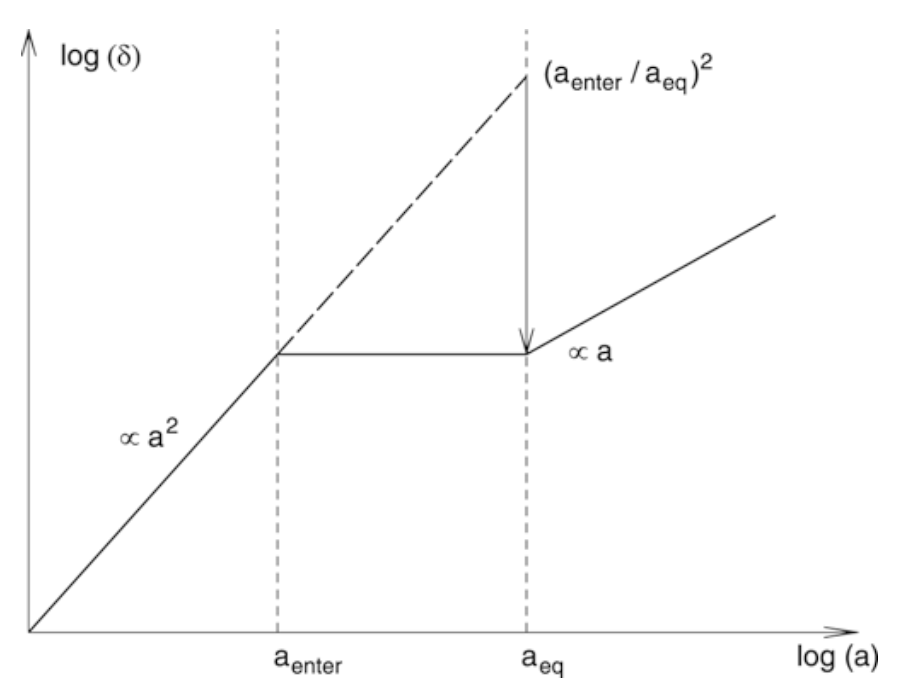
\includegraphics[width=10cm]{figures/DensityContrast.png}}
\end{figure}

{\noindent}In linear perturbation theory, fluctuations grow at the same rate on all scales, or for all wave numbers, independent of each other. This applies not only in the Newtonian case, but also remains valid in the framework of General Relativity as long as the fluctuation amplitudes are small. Therefore, the behavior on any (comoving) length-scale can be investigated independently of the other scales. At very early times, perturbations with a comoving scale $L$ are larger than the (comoving) horizon, and only for $z<z_\mathrm{enter}(L)$ does the horizon become larger than the considered scale $L$. Here, $z_\mathrm{enter}(L)$ is defined as the redshift at which the (comoving) horizon equals the (comoving) length-scale $L$,

\begin{align*}
    r_\mathrm{H,com}(z_\mathrm{enter}(L)) = L.
\end{align*}

{\noindent}It is common to say that at $z_\mathrm{enter}(L)$ the perturbation under consideration `enters the horizon', whereas actually the process is the opposite -- the horizon outgrows the perturbation. Relativistic perturbation theory shows that density fluctuations of scale $L$ grow as long as $L>r_\mathrm{H,com}$, namely $\propto a^2$ if radiation dominates (thus, for $z>z_\mathrm{rm}$), or $\propto a$ if matter dominates (i.e., for $z<z_\mathrm{rm}$). Free-streaming particles or pressure gradients cannot impede the growth on scales larger than the horizon length because, according to the definition of the horizon, physical interactions (which pressure or free-streaming particles would be) cannot extend to scales larger than the horizon size.

{\noindent}The evolution of density fluctuations of baryons differs from that of DM. The reason for this is essentially the interaction of baryons with photons: although matter dominates the Universe for $z<z_\mathrm{rm}$, the energy density of baryons remains smaller than that of the photons for a longer time after recombination begins, as can be seen as follows: the baryon-to-photon density ratio is

\begin{align*}
    \frac{\rho_b}{\rho_\gamma} = \frac{\Omega_ba^{-3}}{\Omega_\gamma a^{-4}} = a\frac{\Omega_b\Omega_m\Omega_r}{\Omega_m\Omega_r\Omega_\gamma} = 1.68\frac{a}{a_\mathrm{rm}}\frac{\Omega_b}{\Omega_m} \sim 0.28\frac{a}{a_\mathrm{rm}}.
\end{align*}

{\noindent}Hence, if radiation-matter equality happens at $z_\mathrm{rm}\sim3,000$, then the photon density is larger than that of the baryons for $z\gtrsim800$.

{\noindent}Since photons and baryons interact with each other by photon scattering on free electrons, which again are tightly coupled electromagnetically to protons and helium nuclei, baryons and photons are strongly coupled before recombination, and form a single fluid. Due to the presence of photons, this fluid has a strong pressure, which prevents it from falling into potential wells formed by the dark matter. Thus, the pressure prevents strong inhomogeneities of the baryon-photon fluid.

{\noindent}To discuss the evolution of baryon perturbations in a bit more detail, we consider again a perturbation of comoving scale $L$. As long as the perturbation is larger than the horizon size, pressure effects can not affect the behavior of the fluid, and thus baryons and photons behave in the same way as the dark matter -- the amplitude of their perturbations grow. As soon as the perturbation enters the horizon, the situation changes. Although the baryons are gravitationally pulled into the density maxima of the dark matter, pressure provides a restoring force which acts against a compression of the baryon-photon fluid. As a results, this fluid will develop sound waves.

{\noindent}The maximum distance sound waves can
travel up to a given epoch is called the sound horizon.
Loosely speaking, it is given by the product of the sound
speed and the cosmic time. The sound speed in this photon-dominated fluid is given by $c_s\approx c/\sqrt{3}$. Thus, the sound horizon is about a factor of $\sqrt{3}$ smaller than the event horizon. As soon as a perturbation enters the sound horizon, the amplitude of the baryon-photon fluctuations can not grow anymore; instead, the undergo damped oscillations.

{\noindent}The adiabatic sound speed $c_s$ of a fluid is given in general by

\begin{align*}
    c_s = \sqrt{\frac{\partial P}{\partial\rho}} ~ [{\rm m\,s^{-1}}].
\end{align*}

{\noindent}The pressure of the fluid is generated by the photons, $P=c^2\rho_\gamma/3=c^2\rho_c\Omega_\gamma$, and the density is the sum of that of baryons and photons, $\rho=(\Omega_ba^{-3}+\Omega_\gamma a^{-4})\rho_c$. Thus, the sound velocity is

\begin{align*}
    c_s &= \sqrt{\frac{\partial P}{\partial\rho}} \\
        &= \sqrt{\frac{\mathrm{d}P/\mathrm{d}a}{\mathrm{d}\rho/\mathrm{d}a}} \\
        &= \frac{c}{\sqrt{3}}\sqrt{\frac{4\Omega_\gamma a^{-5}}{3\Omega_ba^{-4}+4\Omega_\gamma a^{-5}}} \\
        &= \frac{c}{\sqrt{3(1+\mathcal{R})}},
\end{align*}

{\noindent}where $\mathcal{R}$ is defined to be

\begin{align*}
    \mathcal{R} = \frac{3}{4}\frac{\rho_b}{\rho_\gamma} = \frac{3}{4}\frac{\Omega_b}{\Omega_\gamma}a.
\end{align*}

{\noindent}Note that $\mathcal{R}$ is smaller than unity until recombination, and thus $c_s\approx c/\sqrt{3}$ provides a reasonable first approximation.

{\noindent}At recombination, the free electrons recombined with the hydrogen and helium nuclei, after which there are essentially no more free electrons which couple to the photon field. Hence, after recombination the baryon fluid lacks the pressure support of the photons, and the sound speed drops to zero -- the sound waves do no longer propagate, but get frozen in. Now the baryons are free to react to the gravitational field created by the dark matter inhomogeneities, and they can fall into their potential wells. After some time, the spatial distribution of the baryons is essentially the same as that of the dark matter.

{\noindent}Hence, there is a maximum wavelength of the sound waves, namely the (comoving) sound horizon at recombination,

\begin{align*}
    r_\mathrm{H,com}(z) &= \int\limits_0^t \frac{c\mathrm{d}t}{a(t)} \\ 
    &= \int\limits_0^{(1+z)^{-1}} \frac{c\mathrm{d}a}{a^2H(a)} \\
    &= \int\limits_0^{a_\mathrm{rec}} \frac{c\mathrm{d}a}{\sqrt{3(1+\mathcal{R})}a^2H(a)},
\end{align*}

{\noindent}where we exchanged the speed of light by the speed of sound.

{\noindent}Figure \ref{fig:perturbationevolution} illustrates the physical significance of this length scale, showing the time evolution of an initial density peak of all four components in the Universe. The length scale $r_s$ is the distance the baryon-photon fluid propagates outwards from the initial density peak before baryons and photons decouple, after which the density perturbation of baryons gets frozen. The x-axis shows the comoving radial coordinate, the y-axis displays the density, multiplied by (radius)$^2$. The different snapshots show the spatial distribution of the various species at later epochs. In particular, because the region is overdense in photons, it is overpressured relative to its surroundings. This overpressure must equilibrate by driving a spherical sound wave out into the baryon-photon plasma which propagates at the speed of sound, $c_s\approx c/\sqrt{3}$. Neutrinos freely stream out of the perturbation at the speed of light. The photon and baryons are strongly coupled before recombination, and thus have the same spatial distribution. At the time of decoupling, the wave stalls as the pressure supplying the photons escape and the sound speed plummets. One ends up with a CDM overdensity at the center and a baryon overdensity in a spherical shell $150$ comoving megaparsecs in radius for the concordance cosmology. At $z\ll10^3$, both of these overdensities attract gas and CDM to them, seeding the usual gravitational instability. However, some of the matter also falls into the density peaks (in the example of this figure, it is an overdense spherical shell) created by baryons, whereas the density profile of neutrinos and photons becomes flat. At late times, the distributions of baryons and dark matter become identical (before the onset of non-linear processes such as halo formation). The central density peak, and the secondary peak have a well-defined separation, given by the distance a sound wave could travel before the baryons decoupled from the photons. Galaxies are more likely to form in these overdensities. The radius of the sphere marks a preferred separation of galaxies, which we quantify as a peak in the correlation function on this scale.

{\noindent}The Universe is of course a superposition of these point-like perturbations, but as the perturbation theory is exquisitely linear at high redshift, we can simply add the solutions. The width of the acoustic peak is set by three factors: silk damping due to photons leaking out of the sound wave, adiabatic broadening of the wave as the sound speed changes because of the increasing inertia of the baryons relative to the photons, and the correlations of the initial perturbations.

\begin{figure}[t!]
    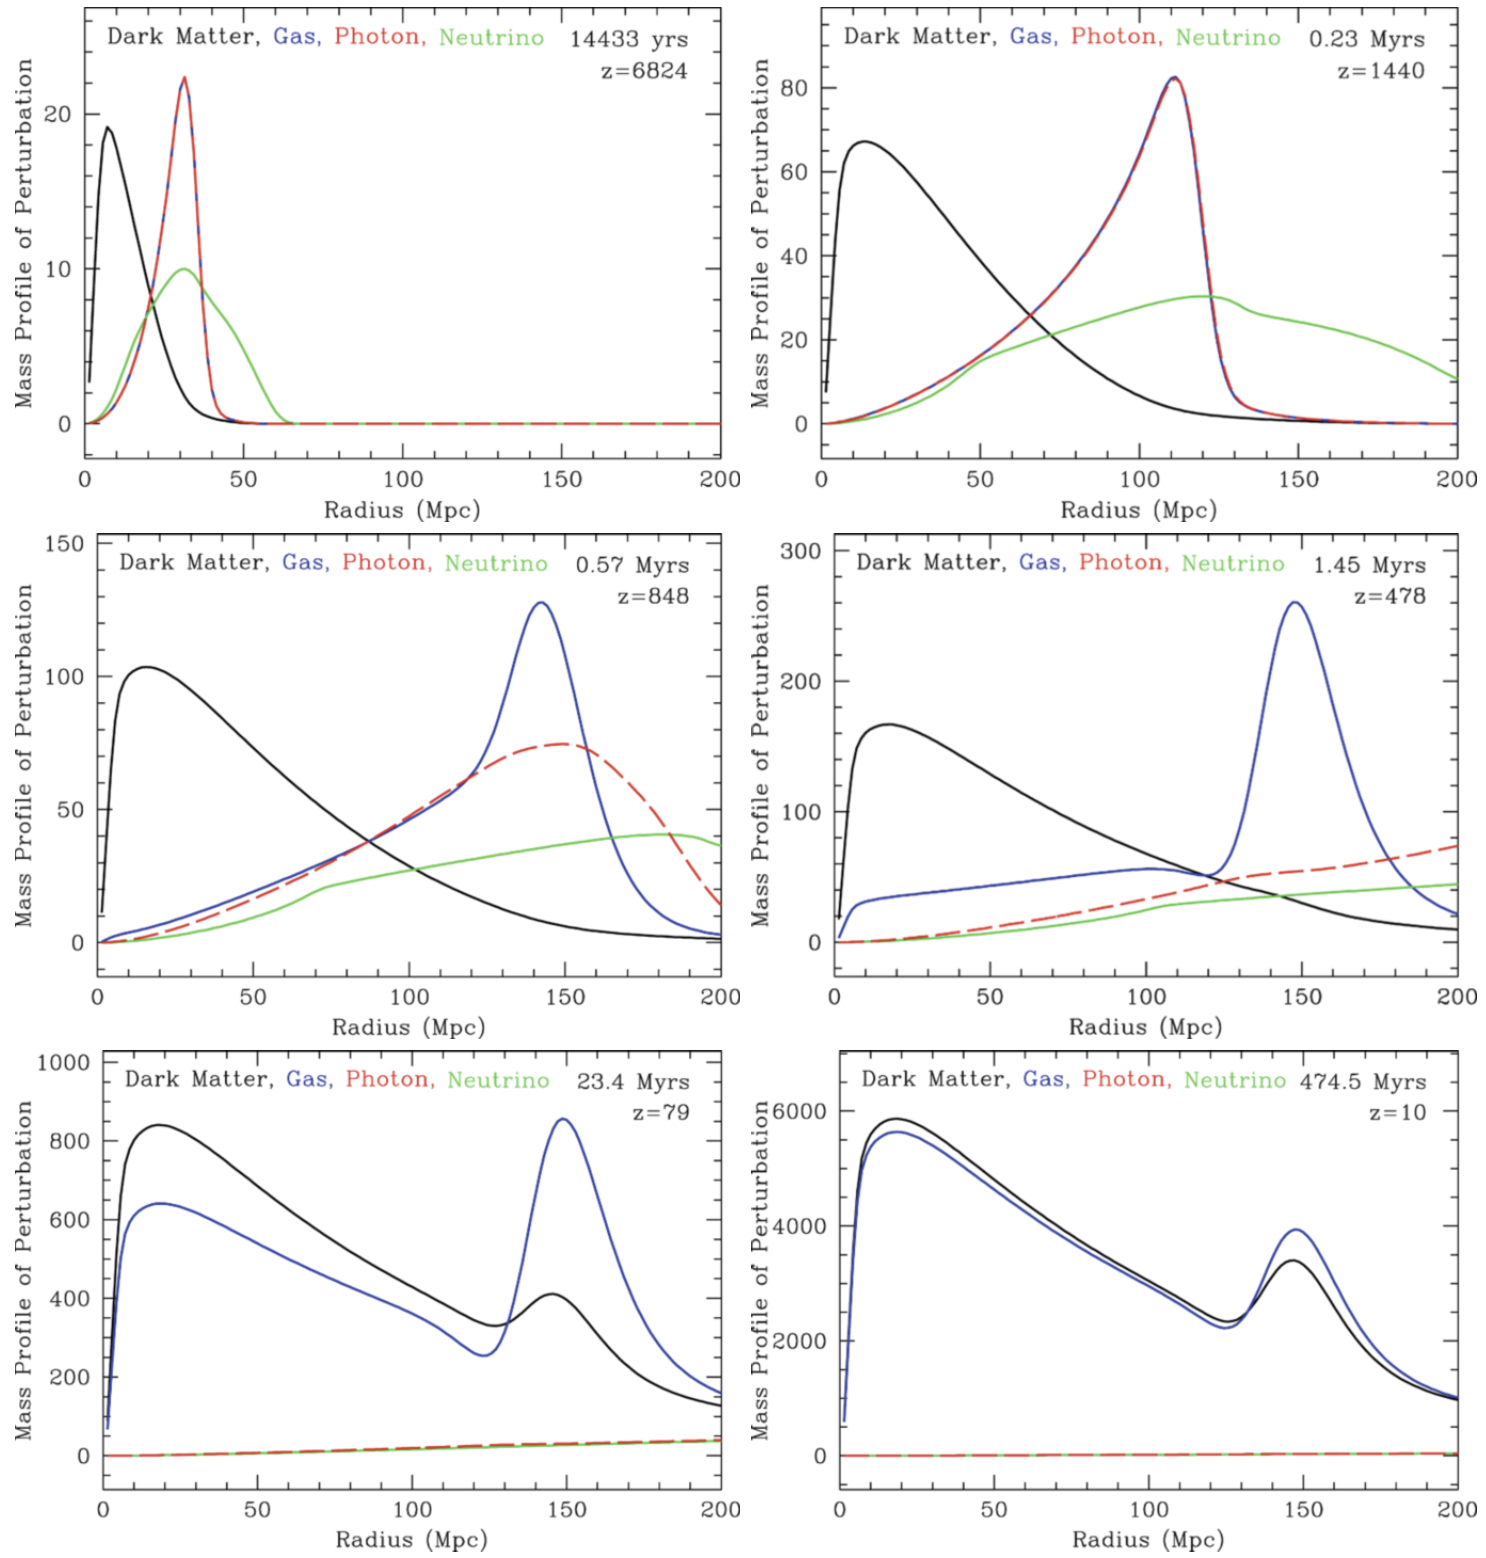
\includegraphics[width=15cm]{figures/PerturbationEvolution.png}
    \centering
    \caption{\footnotesize{Evolution in time of an initial density peak in all components of the cosmic matter. \textit{Top left}: Near the initial time, the photons and baryons travel outward as a pulse. \textit{Top right}: Approaching recombination, one can see the wake in the cold dark matter raised by the outward-going pulse of baryons and relativistic species. \textit{Middle left}: At recombination, the photons leak away from the baryonic perturbation. \textit{Middle right}: With recombination complete, we are left with a CDM perturbation toward the center and a baryonic perturbation in a shell. \textit{Bottom left}: Gravitational instability now takes over, and new baryons and dark matter are attracted to the overdensities. \textit{Bottom right}: At late times, the baryonic fraction of the perturbation is near the cosmic value, because all of the new material was at the cosmic mean. Source: D.J. Eisenstein et al. 2007, On the Robustness of the Acoustic Scale in the Low-Redshift Clustering of Matter, ApJ 664, 660, p. 662, Fig. 1. Figure taken from Schneider (2006).}}
    \label{fig:perturbationevolution}
\end{figure}

{\noindent}There are some other interesting aspects of the physics of this epoch that are worth mentioning. First is that the outgoing wave does not actually stop at $z\sim10^3$ but instead slows around $z\sim500$. This is partially due to the fact that decoupling is not coincident with recombination but is also because the coupling to the growing mode is actually dominated by the velocity field, rather than the density field, at $z\sim10^3$. In other words, the compressing velocity field in front of the wave actually keys the instability at a later time.

{\noindent}Two other aspects that may be surprising at first
glance are that the outgoing pulse of neutrino overdensity does not actually remain as a delta function, as one might expect for a population traveling radially outward at the speed of light, and that the CDM perturbation does not remain at the origin, as one would expect for a cold species. Both of these effects are due to a hidden assumption in the initial conditions: although the density field is homogeneous everywhere but the origin, the velocity field cannot be for a growing mode. To keep the bulk of the universe homogeneous while growing a perturbation at the origin, matter
must be accelerating toward the center; this acceleration is supplied by the gravitational force from the central overdensity. However, in the radiation-dominated epoch the outward-going pulse of neutrinos and photons is carrying away most of the energy density of the central perturbation. This outward-going pulse decreases the acceleration, causing the inward flow of the homogeneous bulk to deviate from the divergenceless flow and generating the behavior of the CDM and neutrinos mentioned above. Essentially,
the outgoing shells of neutrinos and photons raise a wake in the homogeneous distribution of CDM away from the origin
of the perturbation.

{\noindent}The smoothing of the CDM overdensity from a delta function at the origin is the famous small-scale damping of the CDM power spectrum in the radiation-dominated epoch. The overdensity raised decreases as a function of radius because the radiation is decreasing in energy density relative to the inertia of the CDM; in the matter-dominated regime, the outward-going radiation has no further effect. A universe with more radiation causes a larger effect that extends to larger radii; this corresponds to the shift in the CDM power spectrum with the matter-to-radiation ratio.

{\noindent}Returning to the major conceptual point, that of the shell of overdensity left at the sound horizon, we see immediately that the sound horizon provides a standard ruler. The radius of the shell depends simply on the sound speed and the amount of propagation time. The sound speed is set by the balance of radiation pressure and inertia from the baryons; this is controlled simply by the baryon-to-photon ratio, which is $\Omega_bh^2$. The propagation time depends on the expansion rate in the matter-dominated and radiation-dominated regimes; this in turn depends on the redshift of matter-radiation equality, which depends only on $\Omega_mh^2$ for the standard assumption of the radiation density (i.e., the standard cosmic neutrino and photon backgrounds and nothing else).

{\noindent}The sound waves in the baryon-photon fluid, the baryonic acoustic oscillations (BAOs), are observable today. Since at recombination, the photons interacted with matter for the last time, the CMB radiation provides us with a picture of the density fluctuations at the epoch of recombination. Our observable cosmic microwave sky essentially is a picture of a two-dimensional cut at fixed time (the time of last scattering) through the density field of the baryons. A cut through an ensemble of sound waves shows an instantaneous picture of these waves. Hence, they are expected to be visible in the temperature distribution of the CMB. This is indeed the case: these BAOs imprint one of the most characteristic features on the CMB anisotropies. Since the sound waves are damped once they are inside the sound horizon, the largest amplitude waves are those whose wavelength equals the sound horizon at recombination.

{\noindent}We have argued that the baryons, once they are no longer coupled to radiation and thus become pressureless, fall into the potential wells of the dark matter. This happens because the dark matter fluctuations can grow while the baryonic fluctuations could not due to the photon pressure, and because the mean density of dark matter is substantially larger than that of the baryons. This is almost the full story, but not entirely: baryons make about 15\% of the total matter density, and are therefore not negligible. After recombination, the BAOs are frozen, like standing waves, and thus the total matter fluctuations are a superposition of the dark matter inhomogeneities and these standing waves. Whereas the dark matter dominates the density fluctuations, a small fraction of the matter also follows the inhomogeneities created by the standing waves. Since these waves have a characteristic length scale (the sound horizon at recombination) this characteristic length scale should be visible in the properties of the matter distribution even today. The correlation function of galaxies contains a characteristic feature at the length scale $r_s$. Hence, relics of the sound waves in the pre-recombination era are even visible in the current Universe. The effects of the BAOs are included in the transfer function $T(k)$, which thus shows some low-amplitude oscillations, often called `wiggles'.

{\noindent}The distance that acoustic waves can propagate in the first million years of the Universe is measurable not only in the cosmic microwave background (CMB) anisotropies but also in the late-time clustering of galaxies.

\subsubsection{Follow-up Questions}

\begin{itemize}
    \item How do we observe the power spectrum?
    \item What is its relation to BAOs and the $C_\ell$ power spectrum?
    \item Do we see super-horizon modes (modes larger than the universe's event horizon) in the evolved matter power spectrum?
    \item What actually causes the damping during the radiation-dominated era?
    \item Why do modes outside the horizon grow?
\end{itemize}

% --------------------------------------------------------------
%
%                           4. 
%
% --------------------------------------------------------------

\newpage
\subsection{Question 4}

State and explain three key pieces of evidence for a Big Bang origin for the observable Universe.

\subsubsection{Short answer}

The success of the Big Bang (BB) rests on three observational pillars:

\begin{enumerate}
    \item Hubble's Law exhibiting expansion: The first key observation to the modern era of cosmology that the Universe is expanding. If the Universe is expanding at the present time, then by `turning back the clock' the Universe must have been much smaller in the past. Hence, the BB.
    \item Light element abundances which are in accord with Big Bang nucleosynthesis: When the Universe was still a very hot plasma, the extreme radiation field ensured that any nucleus produced would be immediately photoionized by a high energy photon. As the Universe cooled (via expansion) well below the typical binding energies of nuclei, light elements began to form. Knowing the conditions of the early Universe and the relevant cross sections, one can calculate the expected primordial abundances of these light elements. Such predictions are consistent with measurements.
    \item The blackbody radiation left over from the first few hundred thousand years, the cosmic microwave background: The fact that the early Universe was very hot and dense meant that the baryonic matter was well coupled with the radiation field implying thermal equilibrium (TE) of photons. In TE, photons should follow the blackbody (or Planck) function in which the energy density is only dependent on temperature. As it turns out, the CMB radiation is the most accurate BB curve yet to be measured!
\end{enumerate}

\subsubsection{Additional context}

1. \textbf{Hubble's Law}

{\noindent}We have good evidence that the Universe is expanding. This means that early in its history, the distances between galaxies was smaller than it is today. It's convenient to describe this expansion effect by introducing the \textbf{scale factor} $a$, whose present value is equal to one ($a(t_0)\equiv1$). At earlier times, $a$ was much smaller than it is today -- hence, the Big Bang. 

{\noindent}The first key observation to the modern era of cosmology was the discovery of an expanding Universe. This is popularly credited to Edwin Hubble in 1929, but in fact the honour lies with Vesto Slipher more than 10 years earlier. Slipher was measuring spectra of nebulae whose nature was still under hot debate at that time. Observations of Hubble settled this debate in 1924 when he discovered \textit{Cepheid variables} in M31 (Andromeda) establishing a distance of roughly $1\,{\rm Mpc}$. More than a decade earlier in 1913, Slipher had measured the spectrum of M31 and found that it was approaching Earth at a velocity of over $200\,{\rm km\,s^{-1}}$. Over the next decade, he measured Doppler shifts for dozens of galaxies: with only a few exceptions, they were redshifted. By the time Hubble arrived, the basics of relativistic cosmology were already worked out and predictions existed that galaxy redshifts should increase with distance. It's hard to know how much these influenced Hubble, but by 1929 he had obtained Cepheid distances towards 24 galaxies along with their redshifts and claimed that they followed the empirical linear relationship:

\begin{align*}
    v = H_0 d ~ [{\rm km\,s^{-1}}],
\end{align*}

{\noindent}citing theoretical predictions as a possible explanation. At the time, Hubble estimated $H_0 \approx 500\,{\rm km\,s^{-1}\,Mpc^{-1}}$ because his calibration of Cepheid variables was in error. The best modern value is currently $H_0 = 70\,{\rm km\,s^{-1}\,Mpc^{-1}}$.

\begin{figure}[h]
    \floatbox[{\capbeside\thisfloatsetup{capbesideposition={right,center},capbesidewidth=4cm}}]{figure}[\FBwidth]
    {\caption{\footnotesize{The original Hubble diagram (Hubble, 1929). Velocities of distant galaxies (units should be ${\rm km\,s^{-1}}$) are plotted vs distance (units should be ${\rm Mpc}$). Solid (dashed) line is the best fit to the filled (open) points which are corrected (uncorrected) for the Sun's motion. Image taken from Dodelson (2003).}}
    \label{fig:hubblediagram}}
    {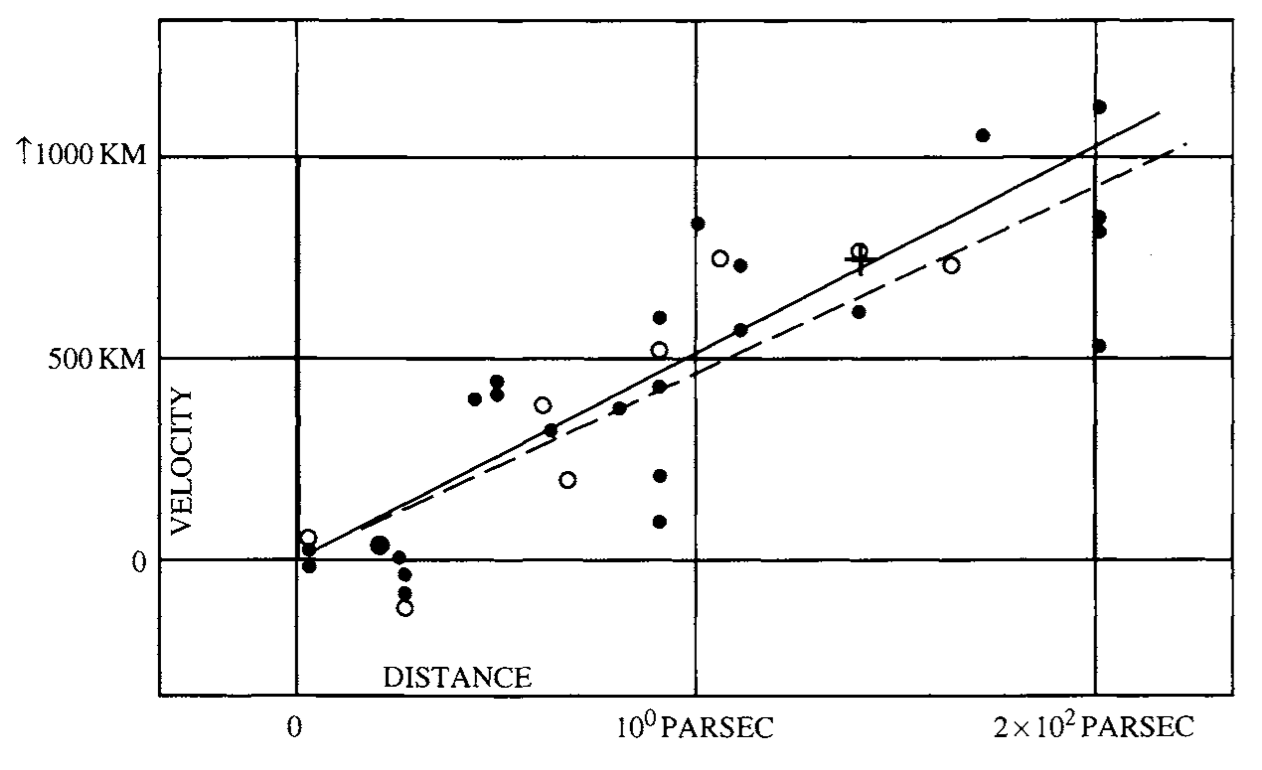
\includegraphics[width=10cm]{figures/HubbleDiagram.png}}
\end{figure}

{\noindent}Recall that the wavelength of light or sound emitted from a receding object is stretched out (i.e., Doppler shifted) so that the observed wavelength is larger than the emitted one. It is convenient to define this stretching factor as the redshift $z$:

\begin{align*}
    1+z \equiv \frac{\lambda_0}{\lambda} = \frac{1}{a} ~ [{\rm dimensionless}],
\end{align*}

{\noindent}or

\begin{align*}
    (1+z)^{-1} \equiv \frac{\lambda}{\lambda_0} = a ~ [{\rm dimensionless}].
\end{align*}

{\noindent}For low redshifts, the standard Doppler formula applies and $z \sim v/c$. Therefore, a measurement of the amount by which absorption and/or emission lines are redshifted is a direct measure of how fast the structures in which they reside are receding from us. Hubble's diagram is shown in Figure \ref{fig:hubblediagram}, which shows not only that distant galaxies appear to be receding from us, but that the trend increases linearly with distance which is exactly what we would expect for an expanding Universe.

{\noindent}The Hubble diagram is still the most direct evidence we have that the universe is expanding. Current incarnations use the same principle as the original: find the distance and the redshift of distant objects. Measuring redshifts is straightforward; the hard part is determining distances for objects of unknown intrinsic brightness. One of the most popular techniques is to try to find a standard candle, a class of objects which have the same intrinsic brightness. Any difference between the apparent brightness of two such objects then is a result of their different distances from us. This method is typically generalized to find a correlation between an observable and intrinsic brightness. For example, \textbf{Cepheid variables} are stars for which intrinsic brightness is tightly related to their pulsation period.

\begin{figure}[h]
    \floatbox[{\capbeside\thisfloatsetup{capbesideposition={right,center},capbesidewidth=4cm}}]{figure}[\FBwidth]
    {\caption{\footnotesize{Hubble diagram from distant Type la supernovae. Top panel shows apparent magnitude (an indicator of the distance) vs redshift. Lines show the predictions for different energy contents in the universe, with $\Omega_M$ the ratio of energy density today in matter compared to the critical density and $\Omega_\Lambda$ the ratio of energy density in a cosmological constant to the critical density. Bottom panel plots the residuals, making it clear that the high-redshift supernovae favor a $\Lambda$-dominated universe over a matter-dominated one. Figure taken from Dodelson (2003).}}
    \label{fig:hubblediagram_modern}}
    {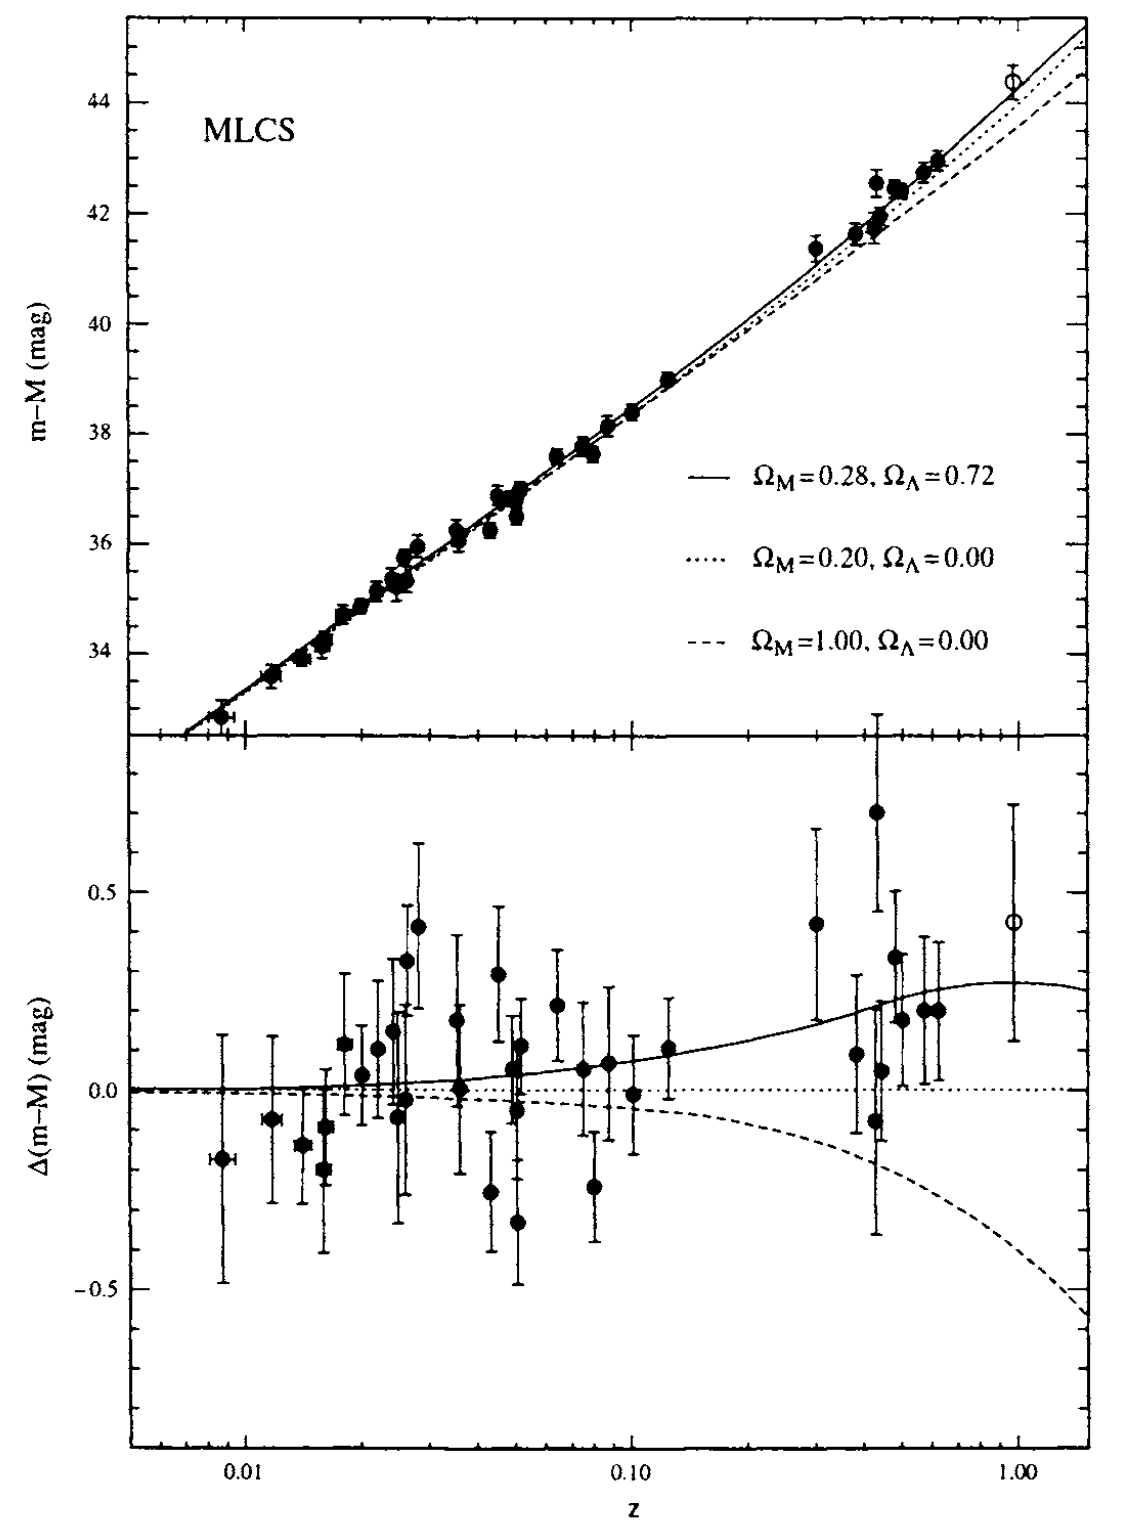
\includegraphics[width=11cm]{figures/HubbleDiagram_modern.png}}
\end{figure}

{\noindent}As seen in Figure \ref{fig:hubblediagram_modern}, the standard candle that can be seen at largest distances is a Type la supernova. Since they are so bright, supernovae can be used to extend the Hubble diagram out to very large redshifts (the current record is of order $z\sim1.7$), a regime where the simple Doppler law ceases to work. Figure \ref{fig:hubblediagram_modern} shows a recent Hubble diagram using these very distant objects. The three curves in Figure \ref{fig:hubblediagram_modern} depict three different possibilities: flat matter dominated; open; and flat with a cosmological constant ($\Omega$). The high-redshift data are now good enough to distinguish among these possibilities, strongly disfavoring the previously favored flat, matter-dominated universe. The current best fit is a universe with about 70\% of the energy in the form of a cosmological constant, or some other form of dark energy.

{\noindent}2. \textbf{Big Bang Nucleosynthesis}

{\noindent}When the universe was much hotter and denser, when the temperature was of order an ${\rm MeV/k_B}$, there were no neutral atoms or even bound nuclei. The vast amounts of radiation in such a hot environment ensured that any atom or nucleus produced would be immediately destroyed by a high energy photon. As the universe cooled well below the binding energies of typical nuclei, light elements began to form. Knowing the conditions of the early universe and the relevant nuclear cross-sections, we can calculate the expected primordial abundances of all the elements.

\begin{figure}[h]
    \floatbox[{\capbeside\thisfloatsetup{capbesideposition={left,center},capbesidewidth=4cm}}]{figure}[\FBwidth]
    {\caption{\footnotesize{BBN predictions of the primordial abundances of light elements as a function of today’s baryon density ($\rho_{b,0}$ lower axis) and the corresponding density parameter $\Omega_b$ where $h=0.65$ was assumed. The vertical extent of the rectangles marks the measured values of the abundances (top: He$^4$, center: D, bottom: Li$^7$). The horizontal extent results from the overlap of these intervals with curves computed from theoretical models. The ranges in $\Omega_b$ that are allowed by these three species do overlap, as is indicated by the vertical strip. The deuterium measurements yield the most stringent constraints for $\Omega_b$. Figure taken from Schneider (2006).}}
    \label{fig:bbn_prediction}}
    {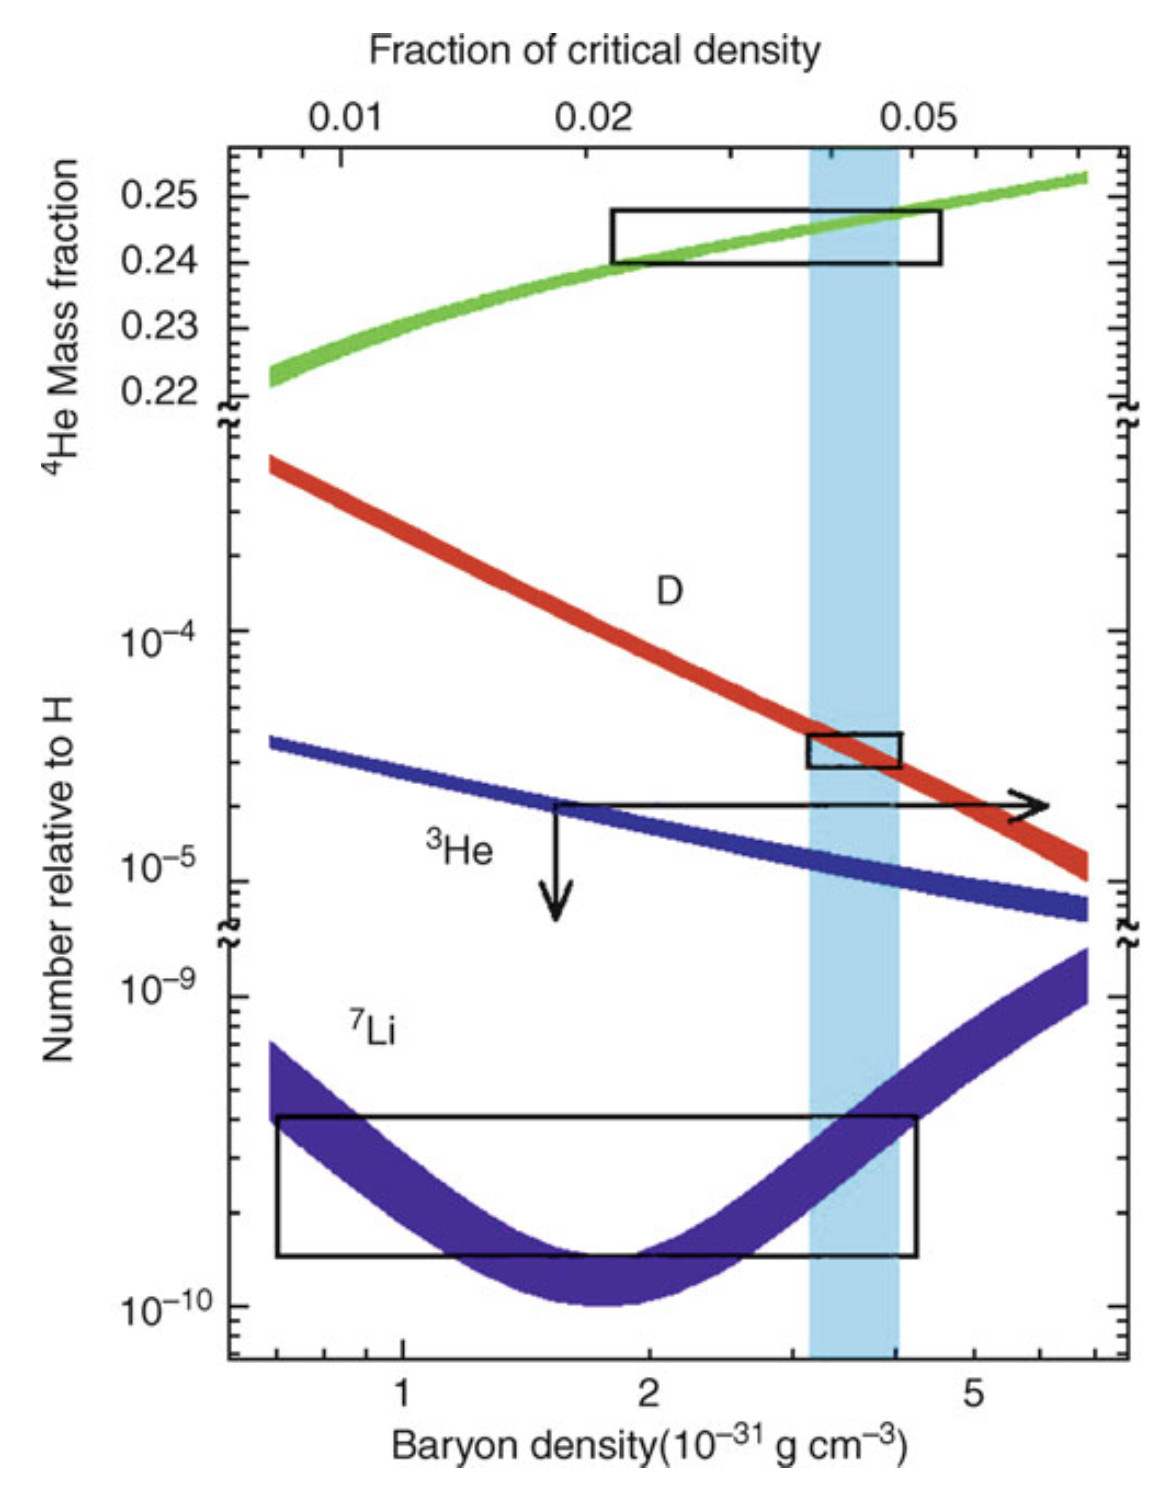
\includegraphics[width=10cm]{figures/BBN_prediction.png}}
\end{figure}

{\noindent}Figure \ref{fig:bbn_prediction} shows the predictions of Big Bang Nucleosynthesis (BBN) for the light element abundances\footnote{Recall nuclear notation: The 4 in $^4$He refers to the total number of nucleons (protons and neutrons). So $^4$He has two neutrons and two protons, while $^3$He has two protons and one neutron.}. The boxes and arrows show the current estimates for the light element abundances. These are consistent with the predictions, and this consistency test provides yet another ringing confirmation of the Big Bang. The theoretical predictions depend on the density of protons and neutrons at the time of nucleosynthesis. The combined proton plus neutron density is called the \textbf{baryon density} ($\rho_b$) since both protons and neutrons have baryon number one and these are the only baryons around at the time. Thus, BBN gives us a way of measuring the baryon density in the universe. Since we know how those densities scale as the universe evolves (they fall as $a^{-3}$), we can turn the measurements of light element abundances into measures of the baryon density today.

{\noindent}In particular, the measurement of primordial deuterium pins down the baryon density extremely accurately to only a few percent of the critical density. Ordinary matter (baryons) contributes at most 5\% of the critical density (i.e., $\Omega_b = 0.005$). Since the total matter density today is almost certainly larger than this -- direct estimates give values of order 20-30\% — nucleosynthesis provides a compelling argument for non-baryonic dark matter.

\begin{figure}[h]
    \floatbox[{\capbeside\thisfloatsetup{capbesideposition={left,center},capbesidewidth=4cm}}]{figure}[\FBwidth]
    {\caption{\footnotesize{Spectrum from a distant QSO (Buries, Nollett, and Turner, 1999). Absorption of photons with rest wavelength $1216$ {\AA} corresponding to the (n = 1) to (n = 2) state of hydrogen is redshifted up to $1216(1+3.572)$ \AA. Bottom panel provides details of the spectrum in this range, with the the presence of deuterium clearly evident. Figure taken from Dodelson (2003).}}
    \label{fig:deuterium}}
    {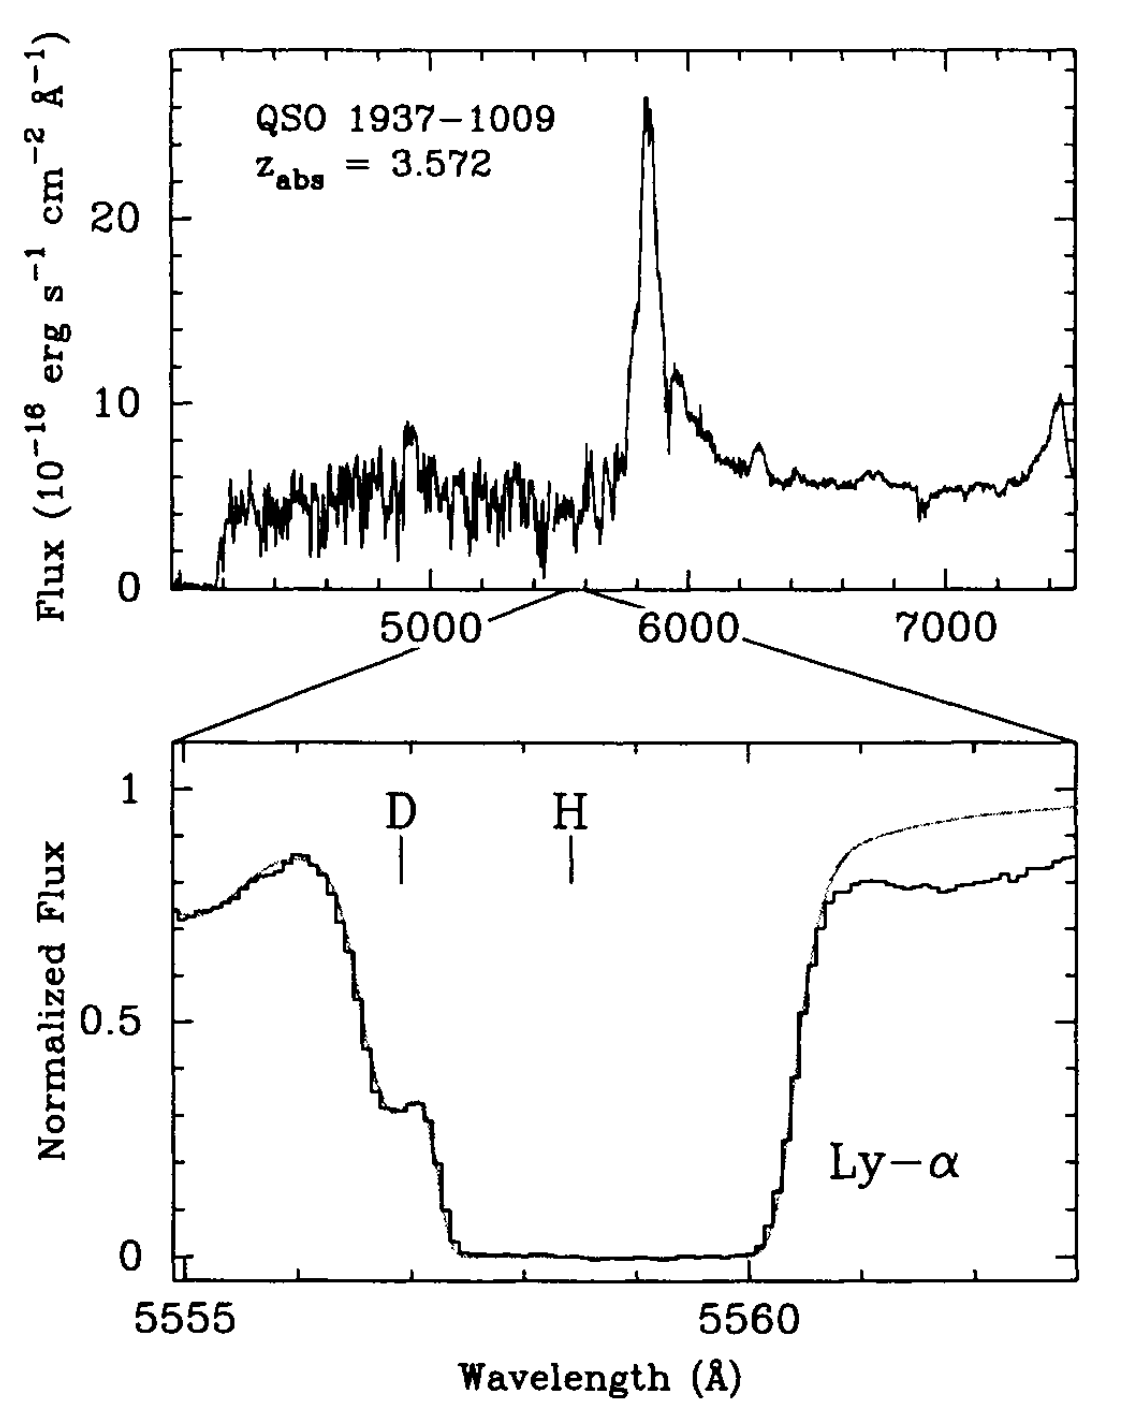
\includegraphics[width=10cm]{figures/deuterium.png}}
\end{figure}

{\noindent}The deuterium measurements (Buries \& Tytler, 1998) are the new developments in the field. These measurements are so exciting because they explore the deuterium abundance at redshifts of order 3-4, well before much processing could have altered the primordial abundances. Figure \ref{fig:deuterium} shows one such detection. The basic idea is that light from distant QSOs is absorbed by intervening neutral hydrogen systems. The key absorption feature arises from transition from the ground state (n=1) of hydrogen to the first excited state (n = 2), requiring a photon with wavelength $\lambda = 1215.7$ \AA. Since photons are absorbed when exciting hydrogen in this fashion, there is a trough in the spectrum at {\AA}, redshifted by a factor of $(1+z)$. The corresponding line from deuterium should be (i) shifted over by $0.33(1+z)$ {\AA} and (ii) much less damped since there is much less deuterium. Figure \ref{fig:deuterium} shows just such a system; there are now half a dozen with detections precisely in the neighborhood shown in Figure \ref{fig:bbn_prediction}. Note that the steep decline in deuterium as a function of baryon density helps here: even relatively large errors in deuterium measurements translate into small errors on the baryon density.

{\noindent}3. \textbf{Cosmic Microwave Background (CMB)}

{\noindent}The CMB offers us a look at the universe when it was only $\sim 380,000$ years old. The photons in the CMB last scattered off electrons at $z \sim 1100$; since then they have traveled freely through space. When we observe them today, they literally come from the earliest moments of time. They are therefore the most powerful probes of the early Universe. If an object is opaque then the protons, neutrons, electrons, and photons which it contains frequently interact and attain \textit{thermal equilibrium}. A crucial fact about the CMB is that the collisions between electrons and photons before last scattering ensured that the photons were in equilibrium. That is, they should have a blackbody spectrum. When a system is in thermal equilibrium, the density of photons in the system as a function of photon energy depends only on the system temperature $T$. It doesn't matter whether the system is a tungsten filament or a sphere of ionized hydrogen and helium.

\begin{figure}[h]
    \floatbox[{\capbeside\thisfloatsetup{capbesideposition={right,center},capbesidewidth=4cm}}]{figure}[\FBwidth]
    {\caption{\footnotesize{Intensity of cosmic microwave radiation as a function of wavenumber from Far InfraRed Absolute Spectrophotometer (FIRAS) (Mather et al., 1994), an instrument on the COBE satellite. Hidden in the theoretical blackbody curve are dozens of measured points, all of which have uncertainties smaller than the thickness of the curve! Figure taken from Dodelson (2003).}}
    \label{fig:cmb_cobe}}
    {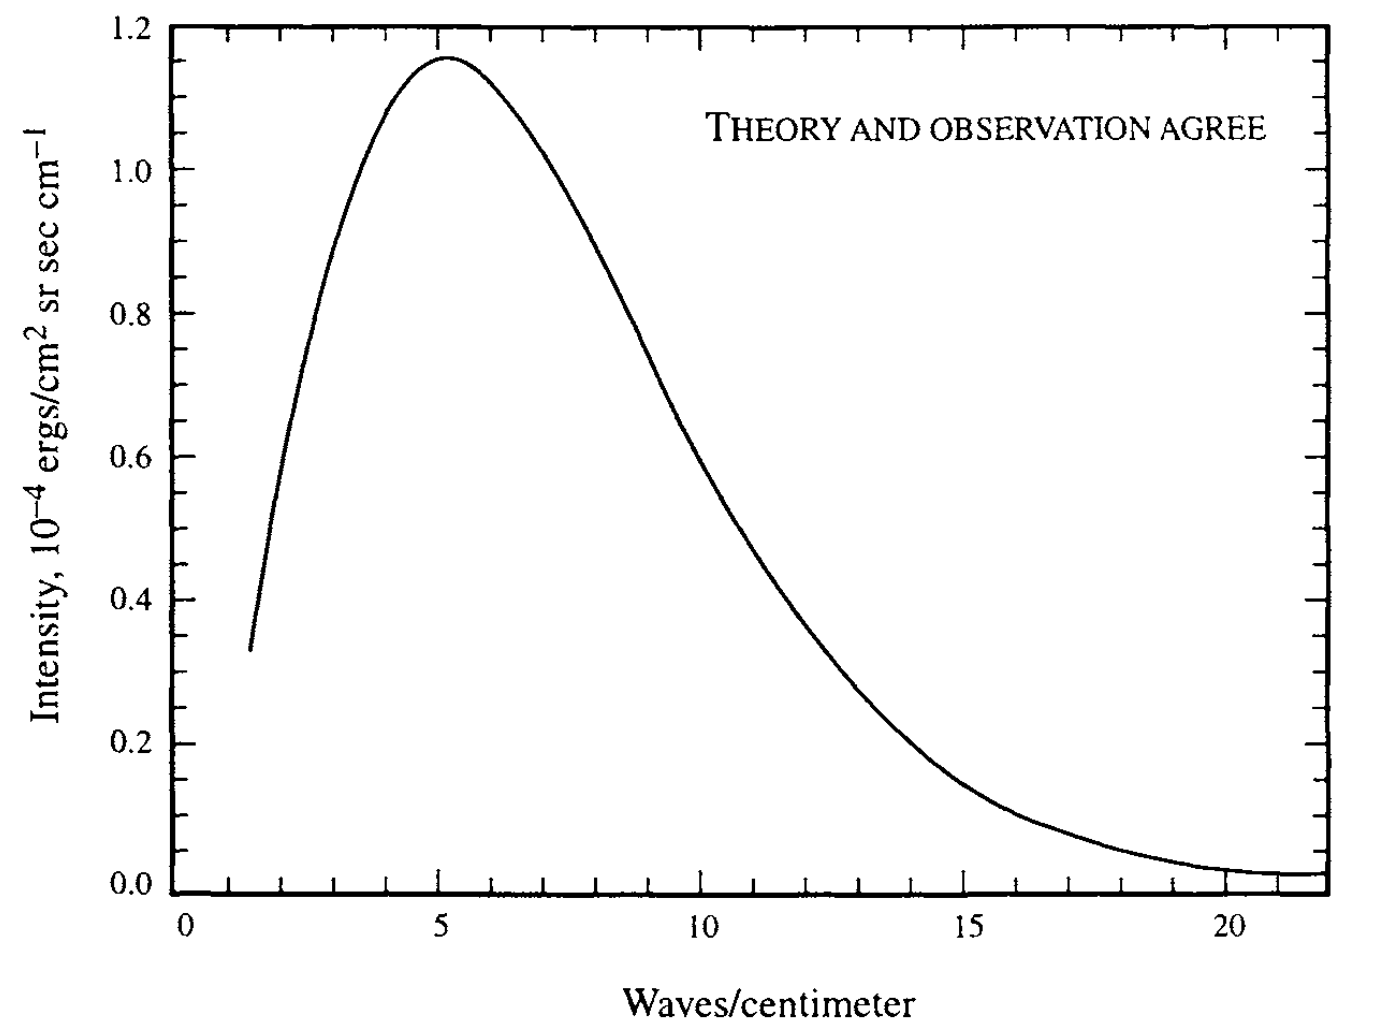
\includegraphics[width=10cm]{figures/CMB_COBE.png}}
\end{figure}

{\noindent}The specific intensity of a gas of photons following a blackbody spectrum is called the \textbf{Planck function}:

\begin{align*}
    I_\nu = B_\nu(T) = \frac{2h\nu^3}{c^2} \frac{1}{\exp({h\nu/k_BT}) - 1} ~ [{\rm erg\,s^{-1}\,cm^{-2}\,Hz^{-1}\,sr^{-1}}].
\end{align*}

{\noindent}Figure \ref{fig:cmb_cobe} shows the remarkable agreement between this prediction of Big Bang cosmology and the observations by the FIRAS instrument aboard the COBE spacecraft. We have been told that detection of the $3\,{\rm K}$ background by Penzias and Wilson in the mid-1960s was sufficient evidence to decide the controversy in favor of the Big Bang over the Steady State universe. Penzias and Wilson, though, measured the radiation at just one wavelength. If even their one-wavelength result was enough to tip the scales, the current data depicted in Figure \ref{fig:cmb_cobe} should send skeptics from the pages of physics journals to the far reaches of radical Internet chat groups.

{\noindent}The photons which make up the cosmic microwave background (CMB) today have a well-measured temperature $T_\mathrm{CMB} = 2.725 \pm 0.002\,{\rm K}$. A photon with an energy $k_BT_\mathrm{CMB}$ today has a wavelength $hc/k_BT_\mathrm{CMB}$. Early on, when the scale factor was smaller than it is today, this wavelength would have been correspondingly smaller. Since the energy of a photon is inversely proportional to its wavelength, the photon energy would have been larger than today by a factor of $1/a$. This argument applied to the thermal bath of photons implies that the temperature of the plasma as a function of time is

\begin{align*}
    T(t) = \frac{T_0}{a(t)} ~ [{\rm K}].
\end{align*}

{\noindent}At early times, then, the temperature was higher than it is today.

{\noindent}The energy density of each component of the Universe is equal to the number density of each corresponding component times its average energy. The primary energy density components of the Universe includes radiation, matter (baryons and dark matter), and dark energy. Since photon energy scales as $a^{-1}$ in addition to the number density which scales as $a^{-3}$, the energy density of radiation should scale as $a^{-4}$. The energy density of non-relativistic particles, such as baryons, have a constant rest mass energy. Since their number density scales inversely proportional to volume, the energy density of matter scales as $a^{-3}$. Dark energy (introduced as a cosmological constant) is believed to have a constant energy density. While matter, and possibly a cosmological constant, dominate the current cosmological landscape, radiation must have been the dominant constituent of the Universe due to its energy density scaling of $a^{-4}$. Figure \ref{fig:energydensityscaling} illustrates how radiation, matter, and the cosmological constant energy density components evolve with time.

\begin{figure}[h]
    \floatbox[{\capbeside\thisfloatsetup{capbesideposition={right,top},capbesidewidth=4cm}}]{figure}[\FBwidth]
    {\caption{\footnotesize{Energy density vs scale factor for different constituents of a flat Universe. Shown are non-relativistic matter, radiation, and a cosmological constant. All are in units of the critical density today. Even though matter and cosmological constant dominate today, at early times, the radiation density was largest. The epoch at which matter and radiation are equal is $a_\mathrm{eq}$. Image taken from Dodelson (2003).}}
    \label{fig:energydensityscaling}}
    {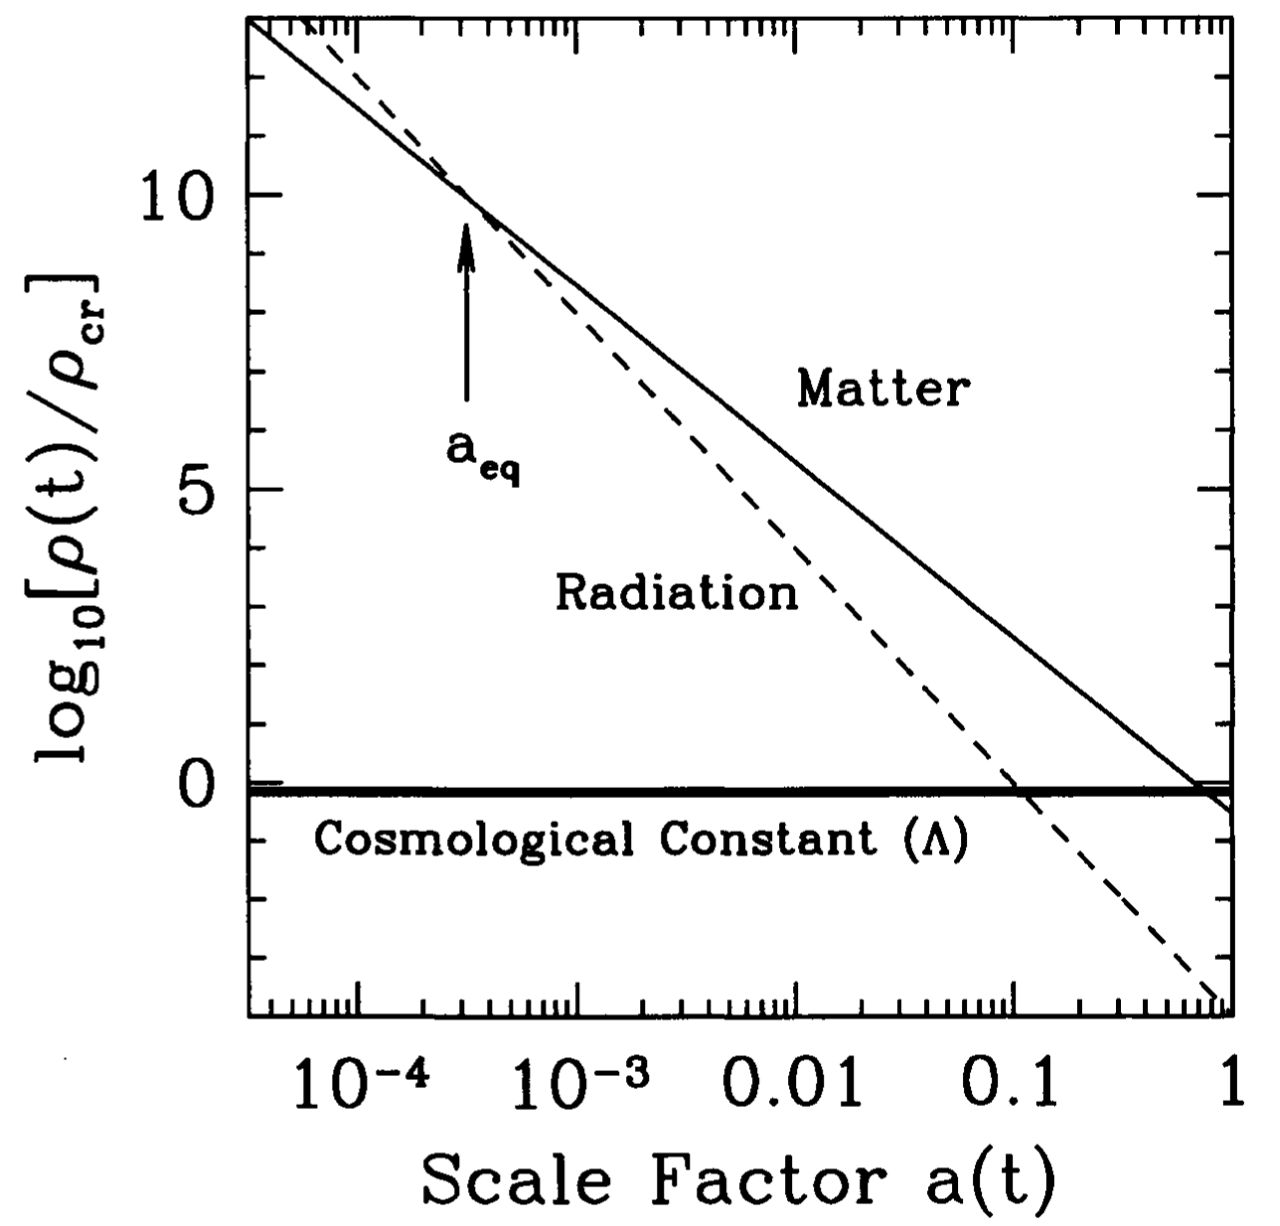
\includegraphics[width=10cm]{figures/EnergyDensityScaling.png}}
\end{figure}

{\noindent}The CMB was detected by Arno Penzias \& Robert Wilson in 1965 and were awarded the 1978 Nobel prize in physics; they accomplished this by locating an unaccounted-for source of noise in a radio telescope at Bell Laboratories being used to study our own Galaxy. This excess ``noise'' was isotropic and constant with time, so it couldn't be associated with an isolated celestial source. Wilson and Penzias were puzzled until they were put into touch with Robert Dicke and his research group at Princeton University. Dicke had deduced that the Universe, if it started in a hot dense state, should now be filled with microwave radiation. The timing of the discovery was especially ironic, given that instruments were underway at that time to test the theoretical prediction that such a background should exist.

{\noindent}When the Universe was fully ionized, photons interacted primarily with electrons via Thomson scattering (the low energy limit of Compton scattering): 

\begin{align*}
    \gamma + e^{-} \rightarrow \gamma + e^{-}.
\end{align*}

{\noindent}Thomson scattering is an elastic process whereby energy and momentum are transferred between the photon and electron. The cross-section for Thomson scattering is the Thomson cross-section of 

\begin{align*}
    \sigma_e = 6.65 \times 10^{-29} ~ [{\rm m^2}].
\end{align*}

{\noindent}The mean free path of a photon -- that is, the mean distance it travels before scattering from an electron-- is therefore

\begin{align*}
    \ell_\mathrm{mfp} = \frac{1}{n_e\sigma_e} ~ [{\rm m}].
\end{align*}

{\noindent}When the baryonic component of the universe is fully ionized, $n_e = n_p = n_b$. Currently, the number density of baryons is $n_{b,0} = 0.22\,{\rm m^{-3}}$. The number density of conserved particles, such as baryons, goes with the scale factor as $1/a^3$, so when the early universe was fully ionized, the free electron density was

\begin{align*}
    n_e = n_b = \frac{n_{b,0}}{a^3} ~ [{\rm m^{-3}}].
\end{align*}

{\noindent}Since photons travel with speed $c$, the rate at which a photon undergoes scattering interactions is

\begin{align*}
    \Gamma = \frac{c}{\ell_\mathrm{mfp}} = n_e\sigma_ec ~ [{\rm s^{-1}}].
\end{align*}

{\noindent}Using the fact that $n_e = n_b = n_{b,0}/a^3$ for a fully-ionized Universe,

\begin{align*}
    \Gamma = \frac{n_{b,0}\sigma_ec}{a^3} = \frac{4.4\times10^{-21}}{a^3} ~ [{\rm s^{-1}}].
\end{align*}

{\noindent}The photons remain coupled to the electrons as long as their scattering rate, $\Gamma$, is larger than $H$, the rate at which the Universe expands; this is equivalent to saying that their mean free path $\ell_\mathrm{mfp}$ is shorter than the Hubble distance $c/H$.

{\noindent}Measuring the spectrum of the CMB, and confirming that it is indeed a blackbody, is not a simple task, even with modern technology. The current energy per CMB photon, $\sim 6 \times 10^{−4}\,{\rm eV}$, is tiny compared to the energy required to break up an atomic nucleus ($\sim 1\,{\rm MeV}$) or even the energy required to ionize an atom ($\sim 10\,{\rm eV}$). However, the mean photon energy is comparable to the energy of vibration or rotation for a small molecule such as H$_2$O. Thus, CMB photons can zip along for more than 13 billion years through the tenuous intergalactic medium, then be absorbed a microsecond away from the Earth’s surface by a water molecule in the atmosphere. Microwaves with wavelengths shorter than λ ∼ 3 cm are strongly absorbed by water molecules.

{\noindent}The CMB can be measured at wavelengths shorter than 3 cm by observing from high-altitude balloons or from the South Pole, where the combination of cold temperatures and high altitude keeps the atmospheric humidity low. The best way to measure the spectrum of the CMB, however, is to go completely above the damp atmosphere of the Earth. The CMB spectrum was first measured accurately over a wide range of wavelengths by the COsmic Background Explorer (COBE) satellite, launched in 1989, into an orbit 900 km above the Earth’s surface. COBE actually contained three different instruments. The Diffuse InfraRed Background Experiment (DIRBE) was designed to measure radiation at the wavelengths 0.001 mm < λ < 0.24 mm; at these wavelengths, it was primarily detecting stars and dust within our own Galaxy. The second instrument, called the Far InfraRed Absolute Spectrophotometer (FIRAS), was used to measure the spectrum of the CMB in the range $0.1\,{\rm mm} < \lambda < 10\,{\rm mm}$, a wavelength band which includes the peak in the CMB spectrum. The third instrument, called the Differential Microwave Radiometer (DMR), was designed to make full-sky maps of the CMB at three different wavelengths: $\lambda = 3.3\,{\rm mm}$, $5.7\,{\rm mm}$, and $9.6\,{\rm mm}$.

{\noindent}The most important fact we learned from our first 25 years of surveying the CMB was that the early Universe was very smooth. No anisotropies were detected in the early CMB. This period, while undoubtedly frustrating for observers searching for anisotropies, solidified the view of a smooth Big Bang. We are now moving on. We have discovered anisotropies in the CMB, indicating that the early Universe was not completely smooth. There were small perturbations in the cosmic plasma. To understand these, we must go beyond the Standard Model.


% --------------------------------------------------------------
%
%                           5. 
%
% --------------------------------------------------------------

\newpage
\subsection{Question 5}

Define and describe the ``tired light hypothesis" and the ``steady state universe'' as alternatives to the Big Bang. How have they been disproved observationally?

\subsubsection{Short answer}

{\noindent}\textbf{Tired Light Hypothesis:} The Tired Light Hypothesis states that the Universe is not expanding, but that photons simply lose energy as they move through space (by some unexplained means). Such a Universe would leads to a blurring of distant objects which is not observed.

{\noindent}\textbf{Steady State Theory:} The Steady State Theory states that matter is continuously being created as the Universe expands in such a way that the matter density remains constant, therefore discarding a beginning to the Universe and adhering to a perfect cosmological principle. The discovery of the Cosmic Microwave Background is commonly regarded as the observation which decisively tipped the scales in favor of the Big Bang model.

\subsubsection{Additional context}

{\noindent}\textbf{Tired Light Hypothesis:} The Tired Light Hypothesis states that the Universe is not expanding, but that photons simply lose energy as they move through space (by some unexplained means), with an exponential dependence on distance $r$ as

\begin{align*}
    E = E_0 \mathrm{e}^{(-r/R_0)} ~ [{\rm eV}],
\end{align*}

{\noindent}where $R_0$ is some constant. There is no known interaction that can degrade a photon's energy without also changing its momentum, which leads to a blurring of distant objects which is not observed.

{\noindent}\textbf{Steady State Theory:} The Steady State model was first proposed in the 1940's by Hermann Bondi, Thomas Gold, and Fred Hoyle, who were proponents of the \textit{perfect cosmological principle}, which states that not only are there no privileged locations in space, there are no privileged moments in time. Thus, a Steady State Universe is one in which the global properties of the universe, such as the mean density $\rho_0$ and the Hubble constant $H_0$, remain constant with time. It was proposed as an alternate theory to the Big Bang model of the Universe which states that matter is continuously being created as the Universe expands in such a way that the matter density remains constant, therefore discarding a beginning to the Universe and adhering to a perfect cosmological principle. Though the Steady State Theory is largely discredited today, its popularity in the 1940's pushed for supporting evidence of the Big Bang model. Interestingly, it was Fred Hoyle who coined the term `Big Bang' during a 1949 BBC interview: ``These theories were based on the hypothesis that all matter in the Universe was created in one big bang at a particular time in the remote past.''

{\noindent}In a Steady State Universe, the velocity-distance relation can be easily integrated:

\begin{align*}
    v &= H_0r ~ [{\rm km\,s^{-1}}]\\
    \frac{dr}{dt} &= H_0r \\
    \int \frac{dr}{r} &= \int H_0 dt \\
    \ln (r) &= H_0t \\
    r(t) &\propto e^{H_0t} [{\rm Mpc}].
\end{align*}

{\noindent}Note that $r \rightarrow 0$ only in the limit that $t \rightarrow -\infty$, so a Steady State Universe is infinitely old. If there existed an instant in time at which the universe started expanding (as in a Big Bang model), that would be a special moment, in violation of the assumed ``perfect cosmological principle''. 

{\noindent}The volume of a spherical region of space, in a Steady State model, increases exponentially with time:

\begin{align*}
    V(t) = \frac{4}{3}\pi r^3 \propto e^{H_0t} = e^{3H_0t} ~ [{\rm Mpc^3}].
\end{align*}

{\noindent}However, if the universe is in a steady state, the density of the sphere must remain constant. To have a constant density of matter within a growing volume, matter must be continuously created at a rate of

\begin{align*}
    \dot{M(t)}_{SS} = \rho_0 \dot{V(t)} = \rho_0 3 H_0 V(t) ~ [{\rm kg\,Gyr^{-1}}].
\end{align*}

{\noindent}If our own universe, with matter density $\rho_0 \sim 3 \times 10^{−27}\,{\rm kg\,m^{−3}}$, happened to be a Steady State universe, then matter would have to be created at a rate of 

\begin{align*}
    \frac{\dot{M(t)}_{SS}}{V(t)} = 3H_0\rho_0 \sim 6\times10^{-29} ~ [{\rm kg\,m^{-3}\,Gyr^{-1}}],
\end{align*}

{\noindent}which corresponds to creating roughly one hydrogen atom per cubic kilometer per year.

{\noindent}The Steady State model finally fell out of favor when observational evidence increasingly indicated that the perfect cosmological principle is not true; the properties of the universe \textit{do}, in fact, change with time. The discovery of the Cosmic Microwave Background is commonly regarded as the observation which decisively tipped the scales in favor of the Big Bang model.

% --------------------------------------------------------------
%
%                           6. 
%
% --------------------------------------------------------------

\newpage
\subsection{Question 6}

Why are only very light elements (H, D, He, and traces of Li) synthesized in the first three minutes of the Big Bang?

\subsubsection{Short answer}

Deuterium synthesis acted as the first bottleneck for nucleosynthesis of heavier elements. The deuteron (i.e., deuterium nucleus) has a binding energy of $2.225\,{\rm MeV}$ which is only $4.3$ times larger than $m_ec^2$ and $1.7$ times larger than the neutron-proton mass-energy difference. Therefore, typical photons are energetic enough to easily photoionize deuterium. The Universe must therefore cool to $T\sim10^9\,{\rm K}$, just below the binding energy of deuterium for the equilibrium to swing in favour of deuterium synthesis. This occurs at $t\sim3\,{\rm min}$. All the while, free neutrons are decaying with a half life of $t_n\sim15\,{\rm min}$. Since the simplest way to synthesize helium is by fusing deuterium, helium synthesis must await significant quantities of deuterium which happens at a temperature roughly one third that at which helium would be expected to dominate. Once significant nucleosynthesis begins, deuterium is rapidly converted into helium owing to its greater binding energy per nucleon ($7\,{\rm MeV}$ as opposed to $1.1\,{\rm MeV}$ for deuterium). This occurs at a temperature of roughly $0.1\,{\rm MeV}$, by which point the density and temperature of the Universe are too low for significant synthesis of heavier nuclei to proceed. 

\subsubsection{Additional context}

{\noindent}At sufficiently early times, the temperature of the Universe was that of the centre of the Sun ($1.55\times10^7\,{\rm K}$), where we know that nuclear reactions occur. Starting in the 1940's, Gamow considered the fascinating question of whether nuclear reactions were possible in the early Universe. He noted that the abundances of some elements in stars showed great regularities, especially a universal proportion of about 25\% helium by mass. This led to the vision that a chain of nuclear reactions in the early Universe could generate not only helium, but all elements. In 1957, the Burbidges, Fowler \& Hoyle showed that almost all elements could in fact be generated in stars, but the problem of helium remained. Gamow showed that its existence could be used to predict the present radiation temperature (as argued below).

{\noindent}It will be convenient to refer to particle masses and temperatures in nuclear physics units, which are ${\rm MeV}$. Some useful conversions are:

\begin{align*}
    1\,{\rm MeV} &= 10^{10.065}\,{\rm K} \\
    m_e &= 0.55\,{\rm MeV} \\
    m_p &= 939\,{\rm MeV} \\
    m_n-m_p &= 1.3\,{\rm MeV}.
\end{align*}

{\noindent}\textit{Neutron freezeout:}

{\noindent}After the annihilation between matter and anti-matter (below $\sim10^{13}\,{\rm K}$), the balance between neutrons and protons are maintained in equilibrium by weak interactions:

\begin{align*}
    p + e^-n \leftrightarrow n + \nu \\
    n + e^+ \leftrightarrow p + \bar{\nu}.
\end{align*}

{\noindent}While this persists, the relative number densities of neutrons and protons should vary according to a Boltzmann factor based on their rest energy difference of $1.3\,{\rm MeV}$:

\begin{align*}
    \frac{n_n}{n_p} = e^{-\Delta mc^2/k_BT} ~ [{\rm dimensionless}].
\end{align*}

{\noindent}The reason that neutrons exist today that the timescale for the weak interactions needed to keep this equilibrium set up eventually becomes longer than the expansion timescale. The reactions thus rapidly cease, and the proton-neutron ratio undergoes freezeout at some characteristic value which determined the He abundance. Since most He is $^4$He (i.e., two neutrons and two protons), the Helium mass fraction (denoted $Y$) is given by

\begin{align*}
    Y = \frac{4\times n_n/2}{n_n + n_p}  = \frac{2}{1 + n_n/n_n} ~ [{\rm dimensionless}]
\end{align*}

{\noindent}neglecting neutrons in other elements. So, $Y=0.25$ requires a neutron-proton freezeout $n_n/n_p\simeq1/7$. To calculate when the neutron-proton ratio undergoes freezeout, we need to know the rates of weak nuclear reactions. Fermi discovered how to calculate the relevant cross sections in the 1930s. Remember that, at $T\sim10^{10}~{\rm K}$, we are above the electron-proton energy threshold, so there exist thermal populations of both electrons and neutrinos to make the reaction $p+e^- \leftrightarrow n+\nu$ go equally well in either direction. All that is needed, therefore, is to consider either the reaction timescale for one proton immersed in a thermal bath of electrons or of one neutron immersed in a bath of neutrinos (the rates are the same). When this timescale equals the local Hubble time, $a(t)/\dot{a}(t)$, we get freezeout of the proton-neutron ratio. Taking the known weak interaction rates, this happens at

\begin{align*}
    T(n~{\rm freezeout}) \simeq 10^{10.14} {\rm K} \Rightarrow \frac{n_n}{n_p} \simeq 0.34.
\end{align*}

{\noindent}This number is not a precisely correct result because nucleosynthesis is a process that contains a number of interesting (but potentially confusing) coincidences:

\begin{enumerate}
  \item The freezeout condition was calculated assuming a temperature well above the electron mass threshold, but freezeout actually happens only a very little above this critical temperature.
  \item Neutrons are not stable: they decay spontaneously with the $e$-folding lifetime of $\tau_n=887\pm2\,{\rm s}$. Unless the frozen-out neutrons can be locked away in nuclei before $t=887\,{\rm s}$, the relic abundance will decay freely to zero. The freezeout point occurs at an age of a few seconds, so there are only a few $e$-foldings of expansion available in which to salvage some neutrinos.
\end{enumerate}

{\noindent}\textit{Locking up the neutrons:}

{\noindent}It may seem implausible that we can add one more coincidence -- i.e., that nuclear reactions will become important at about the same time -- this is just what happens. The Deuteron binding energy of $2.225\,{\rm MeV}$ is only $4.3$ times larger than $m_ec^2$ and only $1.7$ times larger than the neutron-proton mass difference. At higher temperatures, the strong interaction $n+p \leftrightarrow \mathrm{D}+\gamma$ is fast enough to produce deuterium, but thermal equilibrium favours a small deuterium fraction -- i.e., typical photons are energetic enough to disrupt deuterium nuclei very easily. The second key temperature in nucleosynthesis is therefore where the Universe has cooled sufficiently for the equilibrium to swing in favour of deuterium. In practice, this happens at a temperature a little below the deuteron binding energy. This is because the large photon to baryon ratio: even if photons lack sufficient energy to disintegrate deuterons, the rare ones in the tail of the distribution can still do the job. 

{\noindent}Nevertheless, the temperature at which deuterium switches from being rare to dominating the equilibrium is still at $k_BT$ of order the deuterium binding energy:

\begin{align*}
    T({\mathrm{Deuterium~formation}}) \simeq 10^{8.9}\,[{\rm K}],
\end{align*}

{\noindent}or at a time of about 3 minutes.

{\noindent}Notice that we have not needed to know the nuclear reaction rates that form deuterium, since the argument is an equilibrium one. However, if the matter density is too low, the nuclear reactions will freeze out before much deuterium has formed. Gamow took the known nuclear cross-sections and argued that the typical reaction time for deuterium formation had to be the cosmological age at that time (i.e., 3 minutes). This let him conclude that the matter density must have been about $10^{-3}\,{\rm kg\,m^{-3}}$ at that time. This gives a ratio of number densities of photons to nucleons, which is preserved as the Universe expands. Therefore, the present-day matter density allows a prediction of the present-day photon density, and hence its temperature. Alpher \& Herman used Gamow's argument to predict a current photon temperature of $4\,{\rm K}$ to $5\,{\rm K}$, which is impressively accurate. On the other hand, this prediction was based on a figure for the $z=0$ matter density that is probably too low by at least a factor of $100$, raising the temperature estimate by a factor of about 5. Actually, Gamow's argument is an inequality: there is a minimum matter density at $10^9\,{\rm K}$, but it could have been higher. The prediction for the current temperature is therefore really an upper limit. It works because the nuclear reactions are not too far from freeze out when deuterium forms.

{\noindent}The deuterium measurements (Buries and Tytler, 1998) are the new developments in the field. These measurements are so exciting because they explore the deuterium abundance at redshifts of order 3-4, well before much processing could have altered the primordial abundances. Figure \ref{fig:deuterium} shows one such detection. The basic idea is that light from distant QSOs is absorbed by intervening neutral hydrogen systems. The key absorption feature arises from transition from the ground state ($n=1$) of hydrogen to the first excited state ($n=2$), requiring a photon with wavelength $\lambda = 1215.7$ \AA. Since photons are absorbed when exciting hydrogen in this fashion, there is a trough in the spectrum at {\AA}, redshifted by a factor of $(1+z)$. The corresponding line from deuterium should be (i) shifted over by $0.33(1+z)$ {\AA} and (ii) much less damped since there is much less deuterium. Figure \ref{fig:deuterium} shows just such a system; there are now half a dozen with detections precisely in the neighborhood shown in Figure \ref{fig:bbn_prediction}. Note that the steep decline in deuterium as a function of baryon density helps here: even relatively large errors in deuterium measurements translate into small errors on the baryon density.

{\noindent}\textit{Formation of helium:}

{\noindent}The argument so far has produced a Universe consisting of just hydrogen and deuterium, but this is not realistic as one would expect $^4$He to be preferred on thermodynamic grounds, owing to its greater biding energy per nucleon ($7\,{\rm MeV}$ as opposed to $1.1\,{\rm MeV}$ for deuterium). In equilibrium, the first nuclei to come into existence in significant numbers should be $^4$He: the abundance of $^4$He relative to protons should reach unity at an energy of about $0.3\,{\rm MeV}$, at which point the relative abundance of deuterium is only $\sim10^{-12}$.

{\noindent}Since the simplest way to synthesize helium is by fusing deuterium, it is no surprise that the equilibrium prediction fails miserably in the expanding Universe: the production of helium must await the synthesis of significant quantities of deuterium which we have seen happens at a temperature roughly one third that at which helium would be expected to dominate. What the thermodynamic argument does show, however, is that it is expected that deuterium will be rapidly converted to helium once significant nucleosynthesis begins. This argument is what allows us to expect that the helium abundance can be calculated from the final $n_n/n_p$ ratio. The main reactions of importance are of course $2$-body ones, rather than the improbable coincidence of $2$ protons and $2$ neutrons all arriving at the same place simultaneously to make $^4$He in one go. The process starts by fusing deuterium to make either tritium and $^3$He, following which there are four main ways of reaching $^4$He (leaving aside rarer reactions involving residual free neutrons):

\begin{align*}
    \mathrm{D} + \mathrm{D} &\leftrightarrow \mathrm{^3He} + n \\
    \mathrm{D} + \mathrm{D} &\leftrightarrow \mathrm{T} + p \\ \\
    \mathrm{D} + \mathrm{D} &\leftrightarrow \mathrm{^4He} \\
    \mathrm{T} + p &\leftrightarrow \mathrm{^4He} \\
    \mathrm{D} + \mathrm{^3He} &\leftrightarrow \mathrm{^4He} + p \\
    \mathrm{D} + \mathrm{T} &\leftrightarrow \mathrm{^4He} + n.
\end{align*}

{\noindent}The same thermodynamic arguments that say helium should be favoured at temperatures around $0.1\,{\rm MeV}$ say that more massive nuclei would be preferred in equilibrium at lower temperatures still. A Universe that stayed in nuclear equilibrium as it cooled would eventually consist entirely of iron since this has the largest binding energy per nucleon. However, by the time helium synthesis is accomplished, the density and temperature are too low for significant synthesis of heavier nuclei to proceed. Apart from helium, the main nuclear residue of the Big Bang is therefore those deuterium nuclei that escape being mopped up into helium, plus a trace of $^3$He. The other intermediate produce, tritium, is not so strongly bound and and thus leaves no significant relic. There also exists extremely small fractions of other elements: $^7$Li ($\sim10^{-9}$ by mass) and $^7Be$ ($\sim10^{-11}$ by mass). The helium content in the Universe changes later by nuclear fusion in stars, which also forms heavier nuclei (`metals'). However, the total amount of helium produced in stars is expected to be smaller by about one order of magnitude compared to that in BBN.

{\noindent}In summary, nucleosynthesis starts at about $10^{10}\,{\rm K}$ when the Universe was about $1\,{\rm s}$ old, and effectively ends when it has cooled by a factor of 10, and is about 100 times older.

% --------------------------------------------------------------
%
%                           7. 
%
% --------------------------------------------------------------

\newpage
\subsection{Question 7}

Explain how and why Type Ia supernovae are used in the measurements of cosmological parameters.

\subsubsection{Short answer}

Type 1a are good standard candles -- they are very luminous and standardized. The average Type 1a has a peak luminosity of $L=4\times10^9\,\mathrm{L}_\odot$ which is 100,000 times brighter than even the brightest Cepheid variable. When $z\ll1$, the luminosity distance to the light source is

\begin{align*}
    d_L \approx \frac{c}{H_0}z \left(1+\frac{1-q_0}{2}z\right) ~ [{\rm Mpc}]
\end{align*}

{\noindent}The recipe for finding the Hubble constant and deceleration parameters is a simple one:

\begin{itemize}
    \item Measure the redshift $z$ and flux $F$ for each SN.
    \item Compute the luminosity distance $d_L=\sqrt{L/4\pi F}$ for each SN.
    \item Plot the recessional velocity $cz$ versus luminosity distance $d_L$.
    \item Measure the slope of the $cz$ versus $d_L$ relation when $z\ll1$; this gives $H_0$.
    \item At slightly larger values of $z$ (but still $<1$), the deviation of the plot from a straight line tells you the value of $q_0$.
\end{itemize}

\subsubsection{Additional context}

{\noindent}In recent years, the standard candle of choice among cosmologists has been Type Ia supernovae (SNe). A supernova may be loosely defined as an exploding star. Early in the history of supernova studies, when little was known about their underlying physics, supernovae were divided into two classes, on the basis of their spectra. Type I supernovae contain no hydrogen absorption lines in their spectra; Type II supernovae contain strong hydrogen absorption lines. Gradually, it was realized that all Type II supernovae are the same species of beast; they are massive stars ($M>8\,M_\odot$) whose cores collapse to form a black hole or neutron star when their nuclear fuel is exhausted. During the rapid collapse of the core, the outer layers of the star are thrown off into space. Type I supernovae are actually two separate species, which are called Type Ia and Type Ib. Type Ib supernovae, it is thought, are massive stars whose cores collapse after the hydrogen-rich outer layers of the star have been blown away in strong stellar winds. Thus, Type Ib and Type II supernovae are driven by very similar mechanisms -- their differences are superficial, in the most literal sense. Type Ia supernovae, however, are something completely different. They occur in close binary systems where one of the two stars in the system is a white dwarf; that is, a stellar remnant which is supported against gravity by electron degeneracy pressure. The transfer of mass from the companion star to the white dwarf eventually nudges the white dwarf over the Chandrasekhar limit of $1.4\,M_\odot$; this is the maximum mass at which the electron degeneracy pressure can support a white dwarf against its own self-gravity. When the Chandrasekhar limit is exceeded, the white dwarf starts to collapse until its increased density triggers a runaway nuclear fusion reaction. The entire white dwarf becomes a fusion bomb, blowing itself to smithereens; unlike Type II supernovae, Type Ia supernovae do not leave a condensed stellar remnant behind.

{\noindent}Within our Galaxy, Type Ia supernovae occur roughly once per century, on average. Although Type Ia supernovae are not frequent occurrences locally, they are extraordinarily luminous, and hence can be seen to large distances. The luminosity of an average Type Ia supernova, at peak brightness, is $L=4\times10^9\,\mathrm{L}_\odot$; that’s 100,000 times more luminous than even the brightest Cepheid. For a few days, a Type Ia supernova in a moderately bright galaxy can outshine all the other stars in the galaxy combined. Since moderately bright galaxies can be seen at $z\sim1$, this means that Type Ia supernovae can also be seen at $z\sim1$. Not only are Type Ia supernovae bright standard candles, they are also reasonably standardized standard candles. Consider Type Ia supernovae in the Virgo cluster. Although there’s only one Type Ia supernova per century in our own Galaxy, the total luminosity of the Virgo cluster is a few hundred times that of our Galaxy. Thus, every year you can expect a few type Ia supernovae to go off in the Virgo cluster. Several type Ia supernovae have been observed in the Virgo cluster in the recent past, and have been found to have similar fluxes at maximum brightness.

{\noindent}So far, Type Ia supernovae sound like ideal standard candles; very luminous and very standardized. There’s one complication, however. Observation of supernovae in galaxies whose distances have been well determined by Cepheids reveal that Type Ia supernovae do not have identical luminosities. Instead of all having $L = 4\times10^9\,\mathrm{L}_\odot$, their peak luminosities lie in the fairly broad range $L = 3\rightarrow5\times10^9\,\mathrm{L}_\odot$. However, it has also been noted that the peak luminosity of a Type Ia supernova is tightly correlated with the shape of its light curve. Type Ia supernovae with luminosities the shoot up rapidly and decline rapidly are less luminous than average at their peak; supernovae with luminosities which rise and fall in a more leisurely manner are more luminous than average at their peak. Thus, just as the period of a Cepheid tells you its luminosity, the rise and fall time of a Type Ia supernova tells you its peak luminosity.

{\noindent}Recently, two research teams, the ``Supernova Cosmology Project'' and the ``High-z Supernova Search Team'', have been conducting searches for supernovae in distant galaxies. They have used the observed light curves and redshifts of Type Ia supernovae to measure cosmological parameters. First, by observing Type Ia supernovae at $z\sim0.1$, the value of $H_0$ can be determined. The results of the different groups are in reasonable agreement with each other. If the distance to the Virgo cluster is pegged at $d_L = 15\,{\rm Mpc}$, as indicated by the Cepheid results, then the observed supernovae fluxes and redshifts are consistent with $H_0 = 70\pm7\,{km\,s^{-1}\,Mpc^{-1}}$.

{\noindent}In addition, the supernova groups have been attempting to measure the acceleration (or deceleration) of the universe by observing Type Ia supernovae at higher redshift. Before discussing these results, let's introduce the ``magnitude'' system used by astronomers to express fluxes and luminosities. The magnitude system, like much else in astronomy, has its roots in ancient Greece. The Greek astronomer Hipparchus, in the second century BC, divided the stars into six classes, according to their apparent brightness. The brightest stars were of ``first magnitude'', the faintest stars visible to the naked eye were of ``sixth magnitude'', and intermediate stars were ranked as second, third, fourth, and fifth magnitude. Long after the time of Hipparchus, it was realized that the response of the human eye is roughly logarithmic, and that stars of the first magnitude have fluxes (at visible wavelengths) about 100 times greater than stars of the sixth magnitude. On the basis of this realization, the magnitude system was placed on a more rigorous mathematical basis.

{\noindent}Nowadays, the bolometric apparent magnitude of a light source is defined in terms of the source’s bolometric flux as

\begin{align*}
    m \equiv -2.5\log_{10}\left(\frac{F}{F_0}\right) ~ [{\rm mag}],
\end{align*}

{\noindent}where the reference flux $F_0$ is set at the value $F_0 = 2.53\times10^{-8}\,[{\rm W\,m^{-2}}]$. Thanks to the negative sign in the definition, a small value of $m$ corresponds to a large flux $F$. For instance, the flux of sunlight at the Earth’s location is $F = 1367\,[{\rm W\,m^{-2}}]$; the Sun thus has a bolometric apparent magnitude of $m = −26.8$. The choice of reference flux $F_0$ constitutes a tip of the hat to Hipparchus, since for stars visible to the naked eye it typically yields $0 < m < 6$.

{\noindent}The bolometric absolute magnitude of a light source is defined as the apparent magnitude that it would have if it were at a luminosity distance of $d_L = 10\,{\rm pc}$. Thus, a light source with luminosity L has a bolometric absolute magnitude

\begin{align*}
    M \equiv -2.5\log_{10}\left(\frac{L}{L_0}\right) ~ [{\rm mag}],
\end{align*}

{\noindent}where the reference luminosity is $L_0=78.7\,\mathrm{L}_\odot$, since that is the luminosity of an object which produces a flux $F_0 = 2.53\times10^{-8}\,[{\rm W\,m^{-2}}]$ when viewed from a distance of $10\,{\rm pc}$. The bolometric absolute magnitude of the Sun is thus $M = 4.74$. Although the system of apparent and absolute magnitudes seems strange to the uninitiated, the apparent magnitude is really nothing more than a logarithmic measure of the flux, and the absolute magnitude is a logarithmic measure of the luminosity.

{\noindent}Given the definitions of apparent and absolute magnitude, the relation between an object’s apparent magnitude and its absolute magnitude can be written in the form

\begin{align*}
    M = m -5\log_{10}\left(\frac{d_L}{10\,{\rm pc}}\right) ~ [{\rm mag}],
\end{align*}

{\noindent}where $d_L$ is the luminosity distance to the light source. If the luminosity distance is given in units of megaparsecs, this relation becomes

\begin{align*}
    M = m -5\log_{10}\left(\frac{d_L}{1\,{\rm Mpc}}\right)-25 ~ [{\rm mag}].
\end{align*}

{\noindent}Since astronomers frequently quote fluxes and luminosities in terms of apparent and absolute magnitudes, they find it convenient to quote luminosity distances in terms of the distance modulus to a light source. The distance modulus is defined as $m-M$, and is related to the luminosity distance by the relation

\begin{align*}
    m - M = 5\log_{10}\left(\frac{d_L}{1\,{\rm Mpc}}\right)-25 ~ [{\rm mag}].
\end{align*}

{\noindent}The distance modulus of the Large Magellanic Cloud (LMC), for instance, at $d_L = 0.05\,{\rm Mpc}$, is $m - M = 18.5$. The distance modulus of the Virgo cluster, at $d_L = 15\,{\rm Mpc}$, is $m - M = 30.9$. 

{\noindent}Unfortunately, the current proper distance to a Type 1a supernova is not a measurable property. If you tried to measure the distance with a tape measure, for instance, the distance would be continuously increasing as you extended the tape. To measure the proper distance at time $t_0$, you would need a tape measure which could be extended with infinite speed; alternatively, you would need to stop the expansion of the universe at its current scale factor while you measured the distance at your leisure. Neither of these alternatives is physically possible.

{\noindent}Since cosmology is ultimately based on observations, if we want to find the distance to a galaxy, we need some way of computing a distance from that galaxy’s observed properties. For objects at cosmological distances, we can measure the flux of light, $F$, from the object. The complete flux, integrated over all wavelengths of light, is called the bolometric flux. (A bolometer is an extremely sensitive thermometer capable of detecting electromagnetic radiation over a wide range of wavelengths; it was invented in 1881 by the astronomer Samuel Langley, who used it to measure solar radiation.) More frequently, given the difficulties of measuring the true bolometric flux, the flux over a limited range of wavelengths is measured. If the light from the object has emission or absorption lines, we can measure the redshift, $z$.

{\noindent}Since Type 1a supernovae are standard candles in the sense that their luminosities can be measured, then you can use its measured flux $F$ to define a function called the luminosity distance:

\begin{align*}
    d_L \equiv \sqrt{\frac{L}{4\pi F}} ~ [{\rm Mpc}].
\end{align*}

{\noindent}The function $d_L$ is called a ``distance'' because its dimensionality is that of a distance, and because it is what the proper distance to the standard candle would be if the Universe were static and Euclidean. In a static Euclidean universe, the propagation of light follows the inverse square law $F = L/(4\pi d^2)$.

{\noindent}Suppose, though, that you are in a Universe described by a Robertson-Walker metric:

\begin{align*}
    \mathrm{d}s^2 = - c^2\mathrm{d}t^2 + a(t)^2(\mathrm{d}r^2 + S_\kappa(r)^2\mathrm{d}\Omega^2),
\end{align*}

{\noindent}with 

\begin{align*}
    S_\kappa(r) =
    \left\{
    \begin{aligned}
    R\sin(r/R), ~~~~~& (\kappa = +1) \\
              r,~~~~~& (\kappa = 0) \\
    R\sinh(r/R),~~~~~& (\kappa = -1)
    \end{aligned}
    \right.
    .
\end{align*}

{\noindent}You are at the origin. At the present moment $t = t_0$, you see light that was emitted by a standard candle at comoving coordinate location $(r,\theta,\phi)$ at a time $t_e$. The photons which were emitted at time $t_e$ are, at the present moment, spread over a sphere of proper radius $d_p(t_0) = r$ and proper surface area $A_p(t_0)$. If space is flat $(\kappa=0)$, then the proper area of the sphere is given by the Euclidean relation $A_p(t_0) = 4\pi d_p(t_0)^2 = 4\pi r^2$. More generally, however,

\begin{align*}
    A_p(t_0) = 4\pi S_\kappa(r)^2 ~ [{\rm Mpc^2}].
\end{align*}

{\noindent}When space is positively curved, $A_p(t_0) < 4\pi r^2$, and the photons are spread over a smaller area than they would be in flat space. When space is negatively curved, $A_p(t_0) > 4\pi r^2$, and photons are spread over a larger area than they would be in flat space.

{\noindent}In addition to these geometric effects, which would apply even in a static universe, the expansion of the Universe causes the observed flux of light from a standard candle of redshift $z$ to be decreased by a factor of $(1+z)^{−2}$. First, the expansion of the Universe causes the energy of each photon from the standard candle to decrease. If a photon starts with an emitted energy $E = hc/λ$ when the scale factor is $a(t)$, by the time we observe it when the scale factor is A$a(t_0) = 1$, the wavelength will have grown to

\begin{align*}
    \lambda_0 = \frac{1}{a(t)}\lambda = (1+z)\lambda ~ [{\rm m}],
\end{align*}

{\noindent}and the energy will have fallen to

\begin{align*}
    E_0 = E(1+z)^{-1} ~ [{\rm eV}].
\end{align*}

{\noindent}Second, thanks to the expansion of the Universe, the time between photon detections will be greater. If two photons are emitted in the same direction separated by a time interval $\delta t$, the proper distance between them will initially be $c\delta t$; by the time we detect the photons at time $t_0$, the proper distance between them will be stretched to $c\delta t(1 + z)$, and we will detect them separated by a time interval $\delta t_0 = \delta t(1 + z)$.

{\noindent}The net result is that in an expanding, spatially curved Universe, the relation between the observed flux $F$ and the luminosity $L$ of a distant light source is

\begin{align*}
    F = \frac{L}{4\pi S_\kappa(r)^2(1+z)^2} ~ [{\rm W\,m^{-2}}],
\end{align*}

{\noindent}and the luminosity distance is

\begin{align*}
    d_L = S_\kappa(r)(1+z) ~ [{\rm Mpc}].
\end{align*}

{\noindent}The available evidence indicates that our Universe is nearly flat, with a radius of curvature $R_0$ which is larger than the current horizon distance $d_\mathrm{hor}(t_0)$. Objects with finite redshift are at proper distances smaller than the horizon distance, and hence smaller than the radius of curvature. Thus, it is safe to make the approximation $r \ll R_0$, implying $S\kappa(r) \approx r$. With our assumption that space is very close to being flat, the relation between the luminosity distance and the current proper distance becomes very simple:

\begin{align*}
    d_L(\kappa=0) = r(1+z) = d_p(t_0)(1+z) ~ [{\rm Mpc}].
\end{align*}

{\noindent}Thus, even if space is perfectly flat, if you estimate the distance to a standard candle by using a naive inverse square law, you will overestimate the actual proper distance by a factor $(1 + z)$.

\begin{figure}[h]
    \floatbox[{\capbeside\thisfloatsetup{capbesideposition={right,top},capbesidewidth=4cm}}]{figure}[\FBwidth]
    {\caption{\footnotesize{The luminosity distance of a standard candle with observed redshift $z$. The bold solid line gives the result for the Benchmark Model, the dot-dash line for a flat, $\Lambda$-only Universe, and the dotted line for a flat, matter-only universe. Figure taken from Ryden (2006).}}
    \label{fig:luminositydistance}}
    {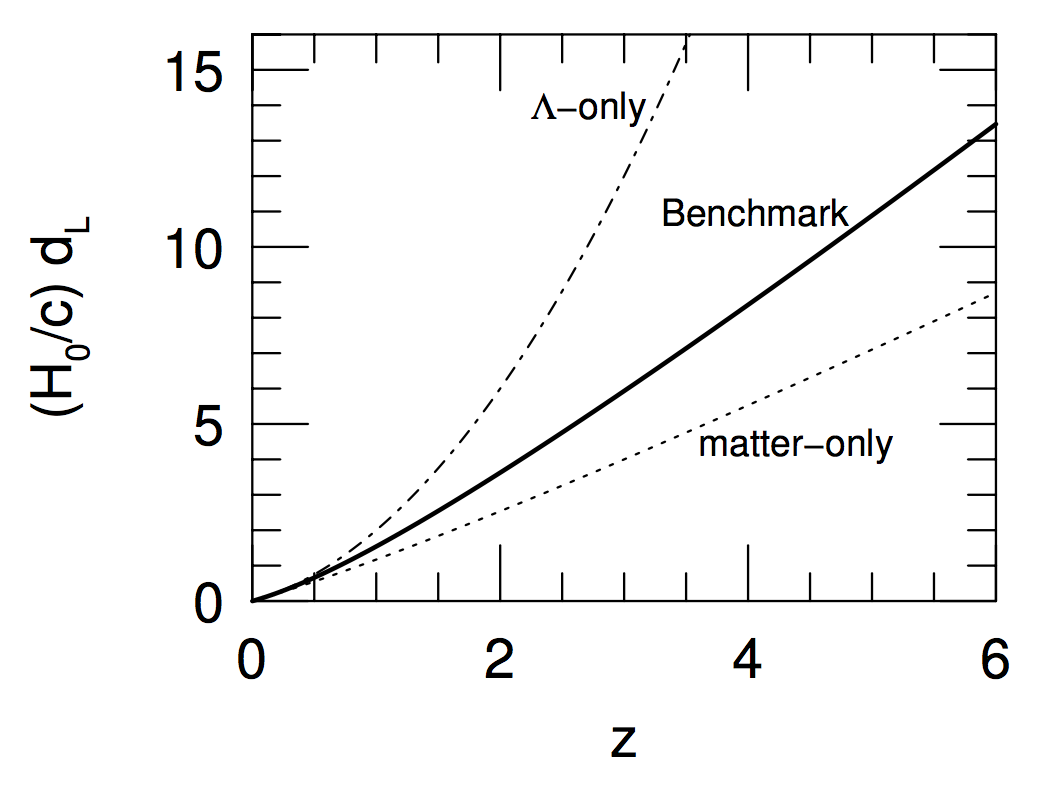
\includegraphics[width=12cm]{figures/LuminosityDistance.png}}
\end{figure}

{\noindent}Figure \ref{fig:luminositydistance} shows the luminosity distance $d_L$ as a function of redshift $z$ for the Benchmark Model, and for two other flat Universes, one dominated by matter and one dominated by a cosmological constant $\Lambda$. When $z \ll 1$, the current proper distance may be approximated as

\begin{align*}
    d_p(t_0) \approx \frac{c}{H_0}z \left(1-\frac{1+q_0}{2}z\right) ~ [{\rm Mpc}].
\end{align*}

{\noindent}In a universe which is nearly flat, the luminosity distance may thus be approximated as

\begin{align*}
    d_L &\approx \frac{c}{H_0}z \left(1-\frac{1+q_0}{2}z\right)(1+z) \\
        & \approx \frac{c}{H_0}z \left(1+\frac{1-q_0}{2}z\right).
\end{align*}

{\noindent}Note that in the limit $z\rightarrow0$,

\begin{align*}
    d_p(t_0) \approx d_L \approx \frac{c}{H_0}z ~ [{\rm Mpc}].
\end{align*}

{\noindent}In a universe described by the Robertson-Walker metric, the luminosity distance is a good approximation to the current proper distance for objects with small redshifts.

{\noindent}Substituting the luminosity distance approximation into the expression for the distance modulus gives us the relation between distance modulus and redshift:

\begin{align*}
    m - M \approx 43.17 - 5\log_{10} \left(\frac{H_0}{70\,{\rm km\,s^{-1}\,Mpc}}\right) + 5\log_{10}z + 1.086(1-q_0)z ~ [{\rm mag}].
\end{align*}

{\noindent}For a population of standard candles with known luminosity $L$ (and hence of known bolometric absolute magnitude $M$), you measure the flux $F$ (or equivalently, the bolometric apparent magnitude $m$) and the redshift $z$. In the limit $z\rightarrow0$, a plot of $m − M$ versus $log_{10}(z)$ gives a straight line whose amplitude at a given value of $z$ tells you the value of $H_0$. At slightly larger values of $z$, the deviation of the plot from a straight line tells you the value of $q_0$. At a given value of $z$, an accelerating universe (with $q_0<0$) yields standard candles with a smaller flux than would a decelerating universe (with $q_0>0$).

\begin{figure*}[h!]
    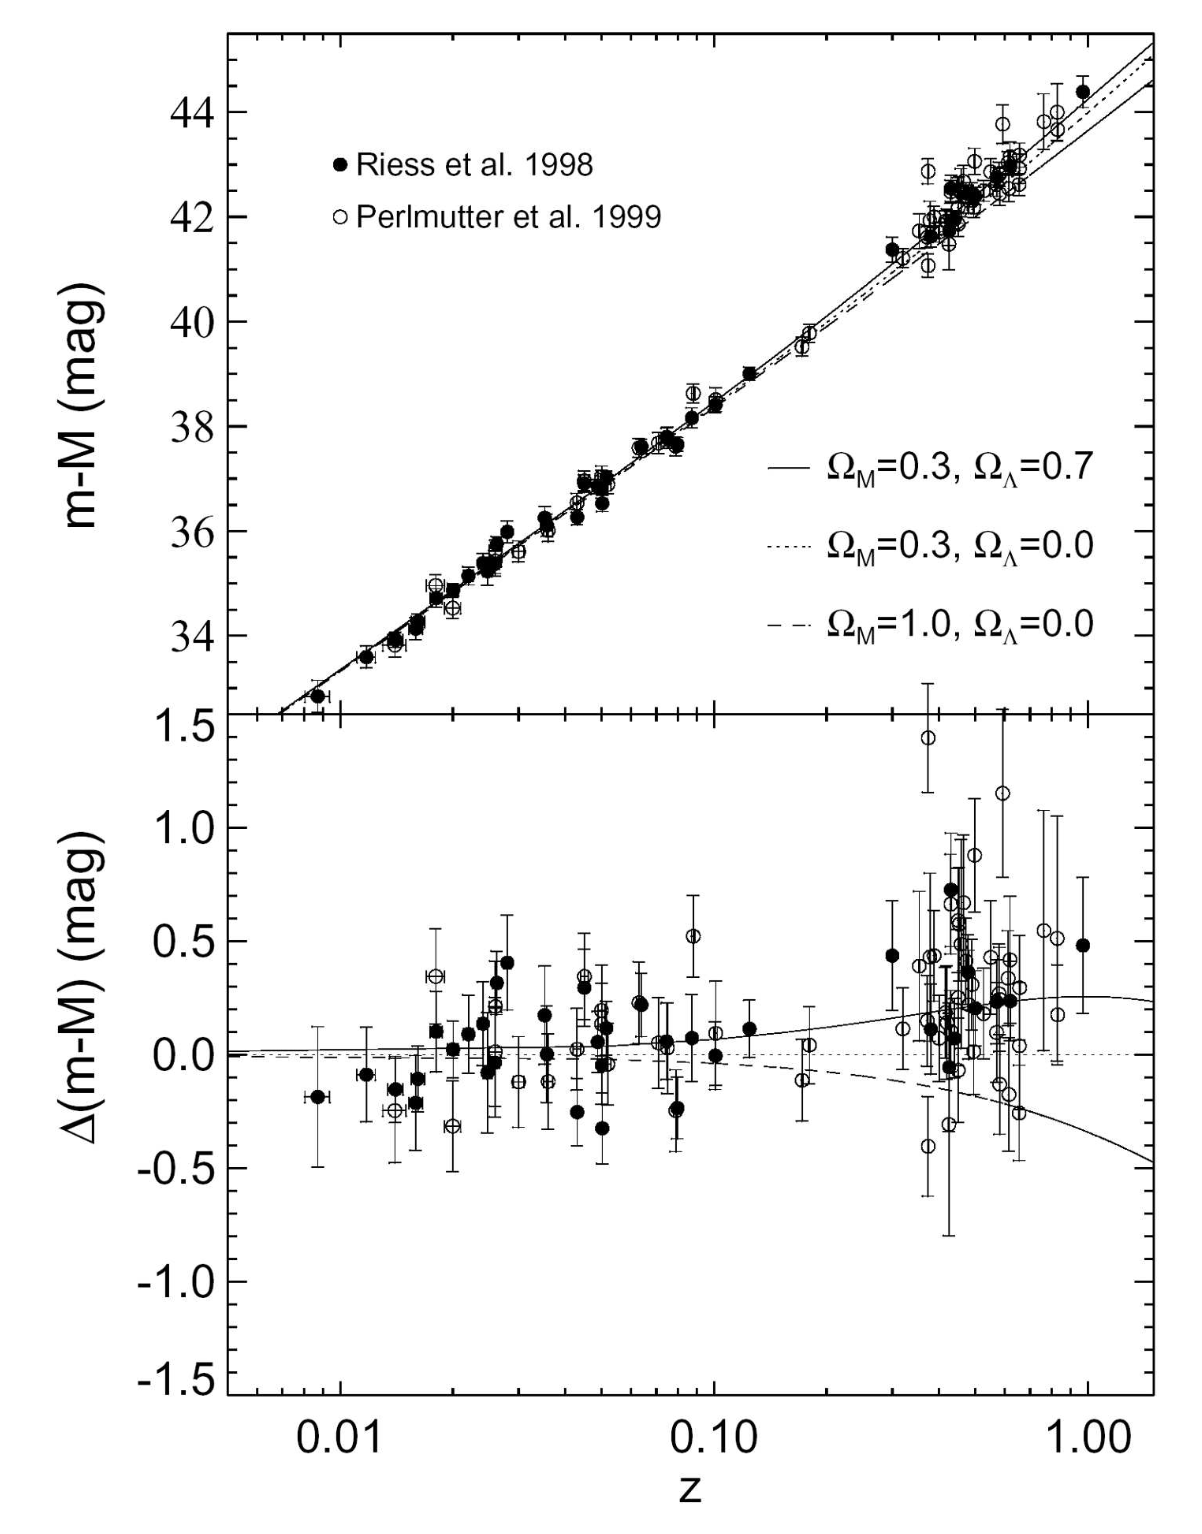
\includegraphics[width=15cm]{figures/DistanceModulus.png}
    \centering
    \caption{Distance modulus versus redshift for Type Ia supernovae from the Supernova Cosmology Project (Perlmutter et al. 1999, ApJ, 517, 565) and the High-z Supernova Search Team (Riess et al. 1998, AJ, 116, 1009). The bottom panel shows the difference between the data and the predictions of a negatively curved $\Omega_{m,0}=0.3$ model (from Riess 2000, PASP, 112, 1284). Figure taken from Ryden (2006).}
    \label{fig:distancemodulus}
\end{figure*}

{\noindent}The upper panel of Figure \ref{fig:distancemodulus} shows the plot of distance modulus versus redshift for the combined supernova samples of the High-z Supernova Search Team (given by the filled circles) and the Supernova Cosmology Project (given by the open circles). The observational results are compared to the expected results for three model Universes. One Universe is flat, and contains nothing but matter $(\Omega_{m,0}=1, q_0=0.5)$. The second is negatively curved, and contains nothing but matter $(\Omega_{m,0}=0.3, q_0=0.15)$. The third is flat, and contains both matter and a cosmological constant $(\Omega_{m,0}=0.3, \Omega_{\Lambda,0}=0.7, q_0=−0.55).$ The data are best fitted by the third of the models -- which is, in fact, our Benchmark Model. The bottom panel of Figure \ref{fig:distancemodulus} shows this result more clearly. It shows the difference between the data and the predictions of the negatively curved, matter-only model. The conclusion that the Universe is accelerating derives from the observation that the supernovae seen at $z \sim 0.5$ are, on average, about $0.25\,{\rm mag}$ fainter than they would in a decelerating universe with $\Omega_{m,0}=0.3$ and no cosmological constant.
 
\begin{figure}[h]
    \floatbox[{\capbeside\thisfloatsetup{capbesideposition={right,top},capbesidewidth=4cm}}]{figure}[\FBwidth]
    {\caption{\footnotesize{The values of $\Omega_{m,0}$ (horizontal axis) and $\Omega_{\Lambda,0}$ (vertical axis) which best fit the data shown in Figure \ref{fig:distancemodulus}. The solid ovals show the best-fitting values for the High-z Supernova Search Team data; the dotted ovals show the best-fitting values for the Supernova Cosmology Project data (from Riess 2000, PASP, 112, 1284) Figure taken from Ryden (2006).}}
    \label{fig:omegamodel}}
    {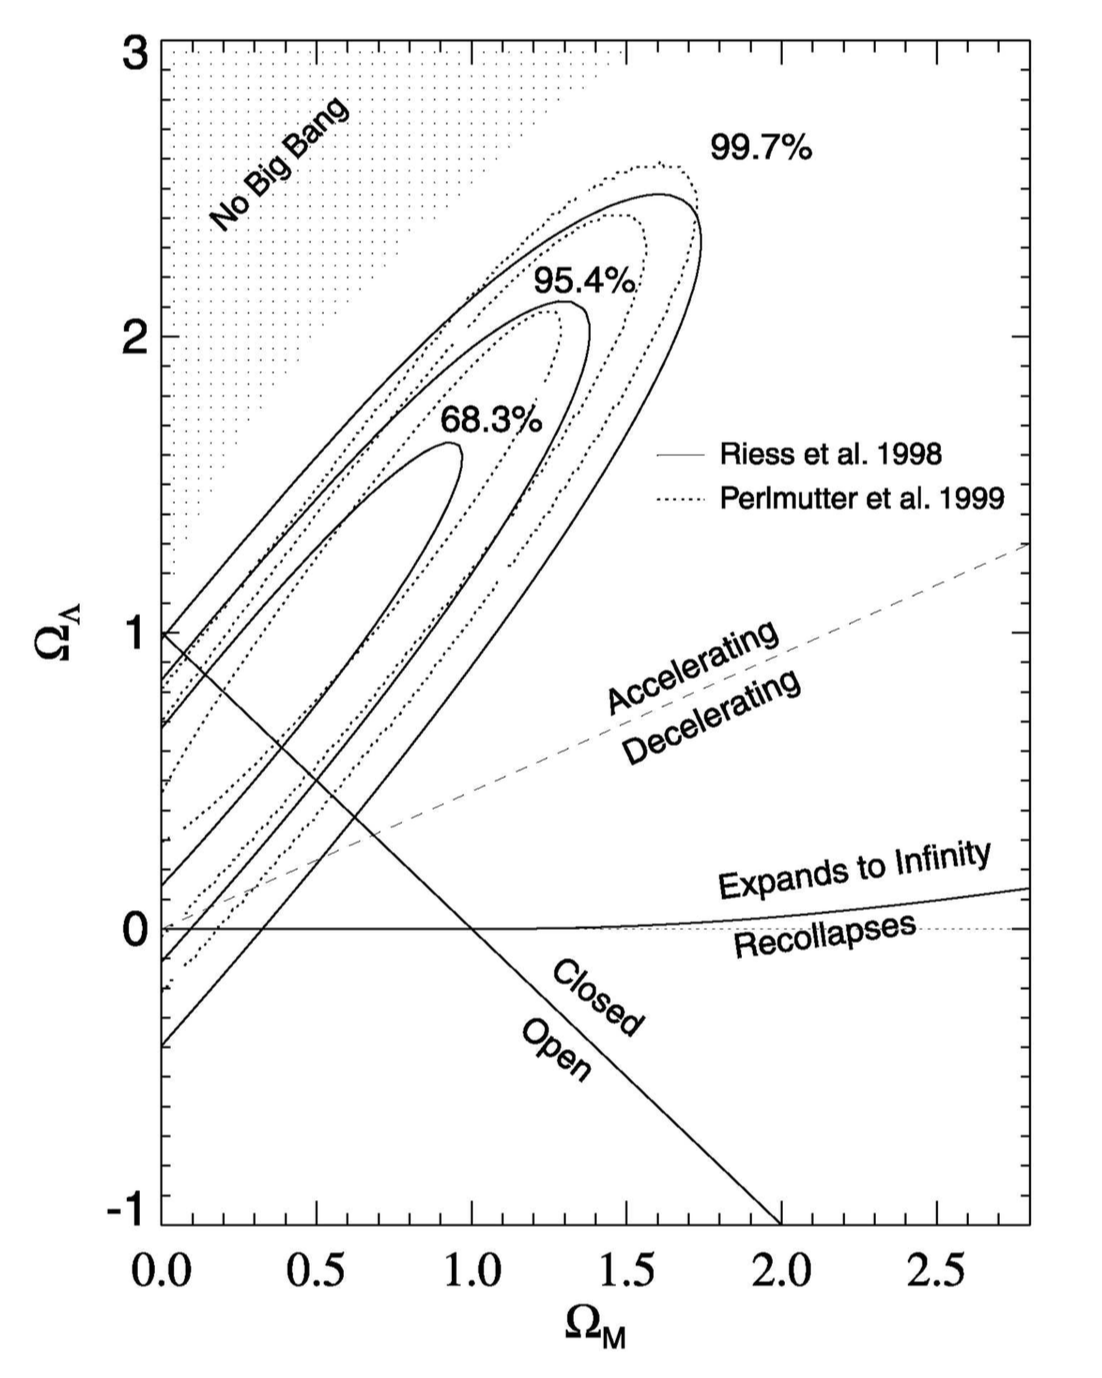
\includegraphics[width=12cm]{figures/OmegaModel.png}}
\end{figure}

{\noindent}The supernova data extend out to $z\sim1$; this is beyond the range where an expansion in terms of $H_0$ and $q_0$ is adequate to describe the scale factor $a(t)$. Thus, the two supernova teams customarily describe their results in terms of a model universe which contains both matter and a cosmological constant. After choosing values of $\Omega_{m,0}$ and $\Omega_{\Lambda,0}$, they compute the expected relation between $m − M$ and $z$, and compare it to the observed data. The results of fitting these model universes are given in Figure \ref{fig:omegamodel}. The ovals drawn on Figure \ref{fig:omegamodel} enclose those values of $\Omega{m,0}$ and $\Omega_{\Lambda,0}$ which give the best fit to the supernova data. The results of the two teams (the solid ovals and dotted ovals) give very similar results. Three concentric ovals are shown for each team’s result; they correspond to $1\sigma$, $2\sigma$, and $3\sigma$ confidence intervals, with the inner oval representing the highest probability. The best fitting models lie along the line $0.8\Omega{m,0} − 0.6\Omega_{\Lambda,0}≈ −0.2.$ Note that decelerating universes (with $q_0>0$) can be strongly excluded by the data, as can Big Crunch universes (labeled `Recollapses' in Figure \ref{fig:omegamodel}), and Big Bounce universes (labeled `No Big Bang' in Figure \ref{fig:omegamodel}). The supernova data are consistent with negative curvature (labeled `Open' in Figure \ref{fig:omegamodel}), positive curvature (labeled `Closed' in Figure \ref{fig:omegamodel}), or with a Universe which is spatially flat.

{\noindent}The results of the supernova teams made headlines when they were first announced; the discovery of the accelerating Universe was named by Science magazine as the `Scientific Breakthrough of the Year' for 1998. It is prudent to remember, however, that all the hoopla about the accelerating Universe is based on the observation that Type Ia supernova at $z\sim.5$ and beyond have somewhat lower fluxes (by about 25\%) than they would have in a decelerating Universe. There are other reasons why their fluxes might be low. For instance, if Type Ia supernovae were intrinsically less luminous at $z\sim0.5$ than at $z\sim0$, that could explain their low fluxes. (If a typical supernova at $z\sim0.5$ had $L=3\times10^9\mathrm{L}_\odot$ rather than $L=4\times10^9\mathrm{L}_\odot$, that would explain their observed dimness, without the need to invoke a cosmological constant. Conversely, if the typical supernova at $z\sim0.5$ had $L=5\times10^9\mathrm{L}_\odot$ rather than $L=4\times10^9\mathrm{L}_\odot$, that would require an even larger cosmological constant to explain their observed dimness.) However, the other properties of Type Ia supernovae, such as their spectra, don’t seem to evolve with time, so why should their luminosity? Perhaps the fluxes of supernovae at $z\sim0.5$ are low because some of their light is scattered or absorbed by intervening dust. However, dust tends to scatter some wavelengths of light more than others. This would change the shape of the spectrum of distant Type Ia supernovae, but no dependence of spectral shape on redshift is observed.

{\noindent}In sum, the supernova results of Figure \ref{fig:omegamodel} provide persuasive evidence for a nearly flat accelerating Universe with $\Omega{m,0}\approx0.3$ and $\Omega_{\Lambda,0}≈ 0.7$.

\subsubsection{Follow-up Questions}

\begin{itemize}
    \item What are Type Ia supernovae (i.e., what is physically happening)?
    \item Can Type Ia constrain all cosmological parameters?
    \item What are some sources of error?
\end{itemize}

% --------------------------------------------------------------
%
%                           8. 
%
% --------------------------------------------------------------

\newpage
\subsection{Question 8}

Describe two methods, other than Type Ia supernovae, by which the cosmological parameters can be determined by astronomical observations.

\subsubsection{Short answer}

Short answer.

\subsubsection{Additional context}

\textbf{CMB Angular Power Spectrum}:

{\noindent}The cosmic microwave background consists of photons that last interacted with matter at $z\sim1,100$. Since the Universe must already have been inhomogeneous at this time, in order for the structures present in the current Universe to be able to form, it is expected that these spatial inhomogeneities are visible as a (small) anisotropy of the CMB: \textit{the angular distribution of the CMB temperature reflects the matter inhomogeneities at the redshift of decoupling of radiation and matter}. The CMB anisotropies reflect the conditions in the Universe at the epoch of recombination, thus at $z\sim1,100$. Temperature fluctuations originating at this time are called \textbf{primary anisotropies}. Later, as the CMB photons propagate through the Universe, they may experience a number of distortions along their way which, again, may change their temperature distribution on the sky. These effects then lead to \textbf{secondary anisotropies}.

{\noindent}Of the primary anisotropies (which directly pertain to inhomogeneities at the time of last scattering) the most basic mechanisms can be divided into those which occur on scales larger than the horizon size at recombination, i.e., which can not have been affected by physical interactions up to the time of last scattering, and those on smaller scales. The effects on superhorizon scales are the following:

\begin{itemize}
    \item \textbf{Sachs-Wolfe effect}: Inhomogeneities in the gravitational potential cause photons which originate in regions of higher density to climb out of a potential well. As a result of this, they lose energy and are redshifted (\textbf{gravitational redshift}). This effect is partly compensated for by the fact that, besides the gravitational redshift, a gravitational time delay also occurs: a photon that originates in an overdense region will be scattered at a slightly earlier time, and thus at a slightly higher temperature of the Universe, compared to a photon from a region of average density. Both effects always occur side by side. This results in photons that are cooler in baryon overdensities. (The dominant one at superhorizon scales.)
    \item \textbf{Peculiar velocities}: The electrons that scatter the CMB photons for the last time do not follow exactly the Hubble expansion, but have an additional velocity that is closely linked to the density fluctuations. This results in a Doppler effect: if photons are scattered by gas receding from us with a speed larger than that corresponding to the Hubble expansion, these photons experience an additional redshift which reduces the temperature measured in that direction.
    \item \textbf{Enhanced baryon density}: The distribution of baryons follows that of the dark matter, so that in regions of a higher dark matter density, the baryon density is also enhanced. This leads to an increased temperature of the baryons in overdense regions.
\end{itemize}

{\noindent}These three effects are relevant on scales larger than the (sound) horizon scale at the epoch of recombination. Obviously, they are closely coupled to each other. In particular, on scales $>r_\mathrm{H,com}(z_\mathrm{rec})$, the first two effects can partially compensate each other, though the Sachs–Wolfe effect is the dominant one at superhorizon scales. Inside the (sound) horizon, two other effects dominate the primary anisotropy signal:

\begin{enumerate}
    \item \textbf{Baryon acoustic oscillations}: On subhorizon scales, the pressure of the baryon-photon fluid is effective because, prior to recombination, these two components had been closely coupled by Compton scattering. This leads to sound waves in the baryon-photon fluid, called the baryonic acoustic oscillations (BAOs). In the density peaks of these sound waves, the baryon-photon fluid is adiabatically compressed and thus hotter than the average. The CMB sky yields a two-dimensional cut through this three-dimensional density (and temperature) field of these sound waves, and thus reflect these fluctuations, yielding temperature anisotropies with characteristic length (or angular) scales. (More on this later.)
    \item \textbf{Silk damping}: The coupling of baryons and photons is not perfect since, owing to the finite mean free path of photons, the two components are decoupled on small spatial scales. This implies that on small length-scales, the temperature fluctuations can be smeared out by the diffusion of photons. This process is known as \textbf{Silk damping}, and it implies that on angular scales below about $\sim50'$, only very small primary fluctuations exist.
\end{enumerate}

{\noindent}\textbf{BAOs}: On subhorizon scales, the pressure of the baryon-photon fluid is effective because, prior to recombination, these two components had been closely coupled by Compton scattering. This leads to sound waves in the baryon-photon fluid, called the baryonic acoustic oscillations (BAOs). In the density peaks of these sound waves, the baryon-photon fluid is adiabatically compressed and thus hotter than the average. The CMB sky yields a two-dimensional cut through this three-dimensional density (and temperature) field of these sound waves, and thus reflect these fluctuations, yielding temperature anisotropies with characteristic length (or angular) scales. 

{\noindent}We expect that these frozen sound waves of the baryons leave an imprint on the overall matter correlation function, best seen in Figure \ref{fig:perturbationevolution}. This unique feature in the correlation function, if it can be detected in the galaxy correlation function, would provide a well-defined `standard rod' in the observable Universe. Since we can observe only angular scales on the sky, the relation between the (comoving) length of the standard rod and the associated angular scale provides a measure of distance. Therefore, a measurement of the baryonic acoustic oscillations (BAOs) in the correlation of galaxies at a given redshift $z$ can be used to determine the (comoving) angular diameter distance $d_A(z)$ --  which depends on the density parameters $\Omega_m$ and $\Omega_\Lambda$.

{\noindent}In fact, the three-dimensional correlation function does not only depend on the transverse length scale which is related to the angular scale via the angular-diameter distance, but also on the separation of galaxies along the line-of-sight. The comoving distance interval corresponding to a redshift interval $\Delta z$ is given by $\Delta x=c\Delta z/H(z)$. Since there are two transversal dimensions, and one along the line-of-sight, the distance measure that is determined best from BAOs is the geometric mean

\begin{align*}
    D(z) = \left(d_A^2(z)\frac{cz}{H(z)}\right)^{1/3}.
\end{align*}

{\noindent}The large redshift surveys 2dFGRS and SDSS allowed the first detection of these BAOs in the galaxy distribution in 2005. Figure \ref{fig:correlationfunction} shows the discovery of BAOs from the SDSS, where a clear feature in the galaxy correlation function is seen at the expected length scale. The mean redshift of the galaxies from which the correlation function was determined is $z\sim0.35$; thus, this measurement yields an estimate of the angular diameter distance to that redshift, with about a 5\% accuracy. In particular, we point out that the sound horizon at recombination is visible in the current Universe!

\begin{figure}[h]
    \floatbox[{\capbeside\thisfloatsetup{capbesideposition={right,top},capbesidewidth=4cm}}]{figure}[\FBwidth]
    {\caption{\footnotesize{The correlation function of galaxies, as observed in the SDSS, shows a clear indication of a secondary peak on a comoving scale of about $100h^{-1}\,{\rm Mpc}\sim150\,{\rm Mpc}$. Curves show models with slightly different density parameter $\Omega_mh^2 = 0.12; 0.13; 0.14$, with fixed baryon density of $\Omega_bh^2=0.024$. The lowest, smooth curve is a  CDM model without baryons which thus shows no features due to baryonic oscillations. Source: D. Eisenstein et al. 2005, Detection of the Baryon Acoustic Peak in the Large-Scale Correlation Function of SDSS Luminous Red Galaxies, ApJ 633, 560, p. 563, Fig. 2. Figure taken from Schneider (2006).}}
    \label{fig:correlationfunction}}
    {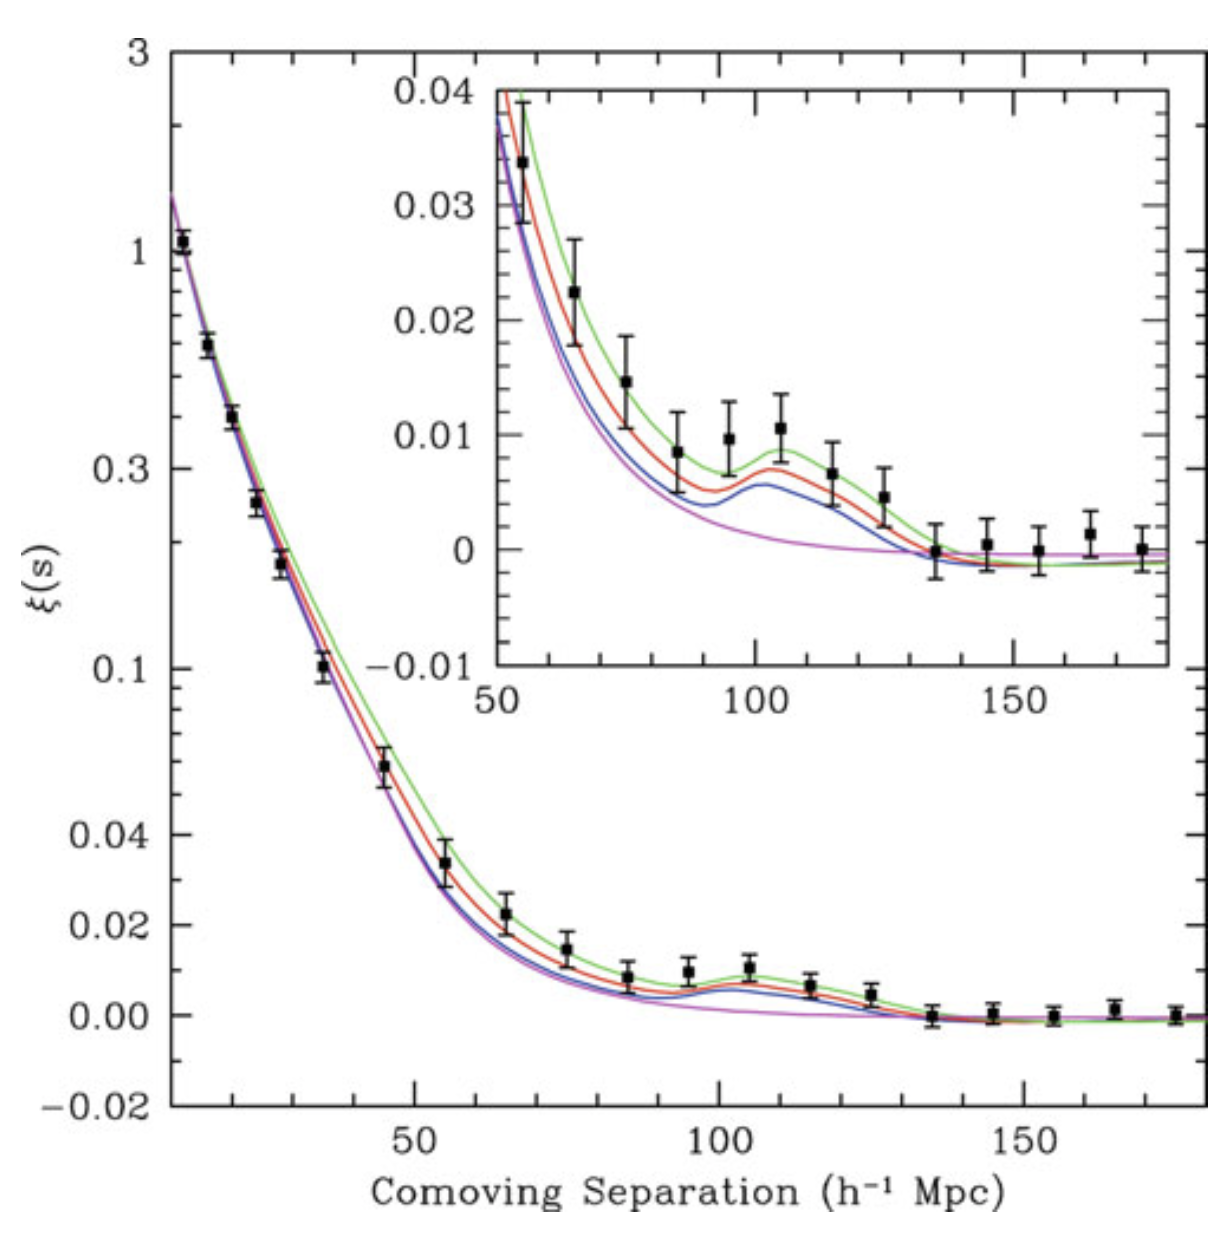
\includegraphics[width=12cm]{figures/CorrelationFunction.png}}
\end{figure}

{\noindent}The power of the method depends on whether the galaxies trace the underlying matter distribution sufficiently well, so that the measured galaxy correlation function reflects the correlation function of matter. Given the large spatial scale on which BAOs are observed, the proportionality between the galaxy and matter fluctuation fields, assumed by the simple bias model, is expected to hold very well. This then turns BAOs into a straightforward, almost purely geometrical tool for measuring the geometry of our Universe.

{\noindent}For this reason, several surveys are underway to measure the acoustic scale as a function of redshift. Figure \ref{fig:BAOs} shows recent measurements of BAOs over a range of redshifts. Amazingly, the measurements are in perfect agreement with the cosmological parameters as determined by CMB anisotropy measurements. In particular, the spatial flatness of our Universe is confirmed, and any curvature is constrained to be very small, $\lvert\Omega_m+\Omega_\Lambda\rvert\lesssim0.01$.

\begin{figure*}[t]
    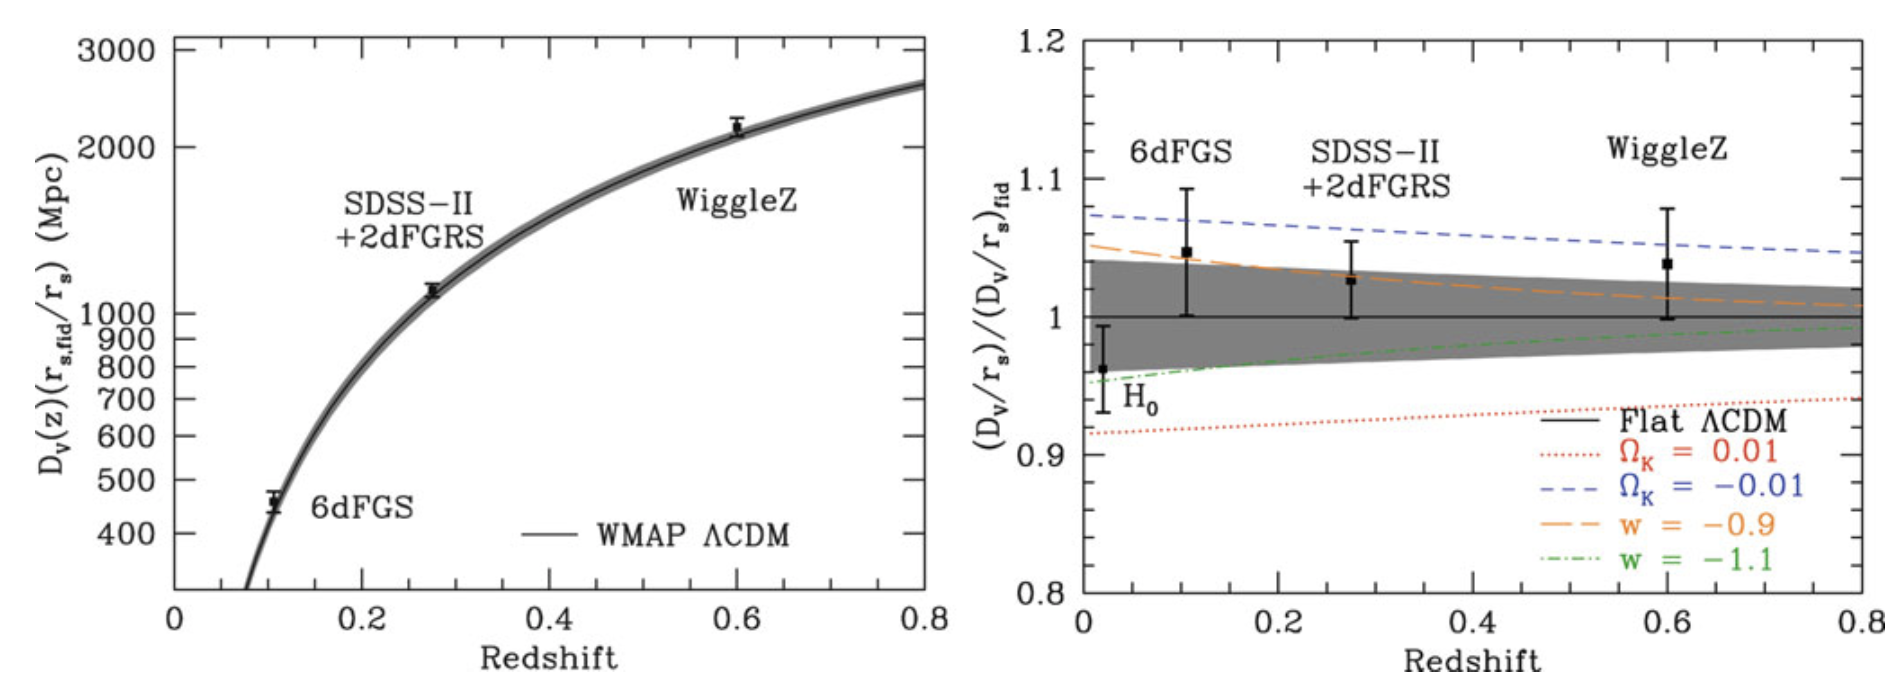
\includegraphics[width=16cm]{figures/BAOs.png}
    \centering
    \caption{\footnotesize{Recent results on the distance-redshift relation from measurements of BAOs. Left panel: The black line and the grey band shows the best-fit cosmological model obtained from the WMAP CMB anisotropy measurements and its $1\sigma$  uncertainty range. The BAO distance determination from three surveys are indicated, which are located right on this best-fit model. Right panel: The same data are shown, now divided by the prediction of a flat $\Lambda$CDM model with parameters as determined from WMAP. Also shown are curves of this distance ratio for models with a small positive or negative curvature, or for different equations-of-state of dark energy. In particular, the BAO measurements exclude any appreciable curvature parameter of our Universe. Source: D.H. Weinberg et al. 2012, Observational Probes of Cosmic Acceleration, arXiv:1201.2434, Fig. 8. Figure taken from Schneider (2006).}}
    \label{fig:BAOs}
\end{figure*}

% --------------------------------------------------------------
%
%                           9. 
%
% --------------------------------------------------------------

\newpage
\subsection{Question 9}

Why is the cosmic microwave background expected to be weakly polarized, and what is practically required to observe this signal?

\subsubsection{Short answer}

The CMB is linearly polarized at the 10\% level due to Thomson scattering of photons off of free electrons at the surface of last scattering.  The degree of linear polarization is directly related to the quadrupole anisotropy in the photons when they last scatter. If the incoming radiation field were isotropic, orthogonal polarization states from incident directions would balance so that the outgoing radiation would remain unpolarized. Conversely, if the incident radiation field possesses a quadrupolar variation in intensity or temperature (which possess intensity peaks at $90^\circ=\pi/2$ separations), the result is a linear polarization of the scattered radiation. No other multipoles other than the quadrupole contributes to the CMB polarization!

\subsubsection{Additional context}

{\noindent}Why should we be concerned with the polarization of the cosmic microwave background (CMB) anisotropies? That the CMB anisotropies are polarized is a fundamental prediction of the gravitational instability paradigm. Under this paradigm, small fluctuations in the early universe grow into the large scale structure we see today. If the temperature anisotropies we observe are indeed the result of primordial fluctuations, their presence at last scattering would polarize the CMB anisotropies themselves. The verification of the (partial) polarization of the CMB on small scales would thus represent a fundamental check on our basic assumptions about the behavior of fluctuations in the Universe, in much the same way that the redshift dependence of the CMB temperature is a test of our assumptions about the background cosmology. Furthermore, observations of polarization provide an important tool for reconstructing the model of the fluctuations from the observed power spectrum (as distinct from fitting an a priori model prediction from observations). The polarization probes the epoch of last scattering directly as opposed to the temperature fluctuations which may evolve between last scattering and the present. This localization in time is a very powerful constraint for reconstructing the sources of anisotropy. Moreover, different sources of temperature anisotropies (scalar, vector, and tensor) give different patterns in the polarization: both in its intrinsic structure and in its correlation with the temperature fluctuations themselves. Thus by including polarization information, one can distinguish the ingredients which go to make up the temperature power spectrum and so the cosmological model. Finally, the polarization power spectrum provides information complementary to the temperature power spectrum even for ordinary (scalar or density) perturbations. This can be of use in breaking parameter degeneracies and thus constraining cosmological parameters more accurately. The prime example of this is the degeneracy, within the limitations of cosmic variance, between a change in the normalization and an epoch of ``late'' reionization.

{\noindent}Yet how polarized are the fluctuations? The degree of linear polarization is directly related to the quadrupole anisotropy in the photons when they last scatter. While the exact properties of the polarization depend on the mechanism for producing the anisotropy, several general properties arise. The polarization peaks at angular scales smaller than the horizon at last scattering due to causality. Furthermore, the polarized fraction of the temperature anisotropy is small since only those photons that last scattered in an optically thin region could have possessed a quadrupole anisotropy. The fraction depends on the duration of last scattering. For the standard thermal history, it is 10\% on a characteristic scale of tens of arcminutes. Since temperature anisotropies are at the $10^{-5}$ level, the polarized signal is at (or below) the $10^{-6}$ level, or several $\mu\mathrm{K}$ representing a significant experimental challenge.

{\noindent}The Thomson scattering cross section $\sigma_T$ depends on polarization as (see, e.g., Chandrasekhar, 1960) as 

\begin{align*}
    \frac{\mathrm{d}\sigma_T}{\mathrm{d}\Omega} \propto \lvert \bm{\epsilon}\cdot\bm{\epsilon}' \rvert^2,
\end{align*}

{\noindent}where $\bm{\epsilon}$ and $\bm{\epsilon}'$ are the incident and scattered polarization directions, and $\Omega$ is the solid angle. Heuristically, the incident light sets up oscillations of the target electron in the direction of the electric field vector $E$ (i.e., the polarization). The scattered radiation intensity thus peaks in the direction normal to, with polarization parallel to, the incident polarization. More formally, the polarization dependence of the cross section is dictated by electromagnetic gauge invariance and thus follows from very basic principles of fundamental physics.

\begin{figure}[h]
    \floatbox[{\capbeside\thisfloatsetup{capbesideposition={right,top},capbesidewidth=4cm}}]{figure}[\FBwidth]
    {\caption{\footnotesize{Thomson scattering of radiation with a quadrupole anisotropy generates linear polarization. Blue colors (thick lines) represent hot and red colors (thin lines) cold radiation. Figure taken from Hu \& White (1997).}}
    \label{fig:Thomsonscattering}}
    {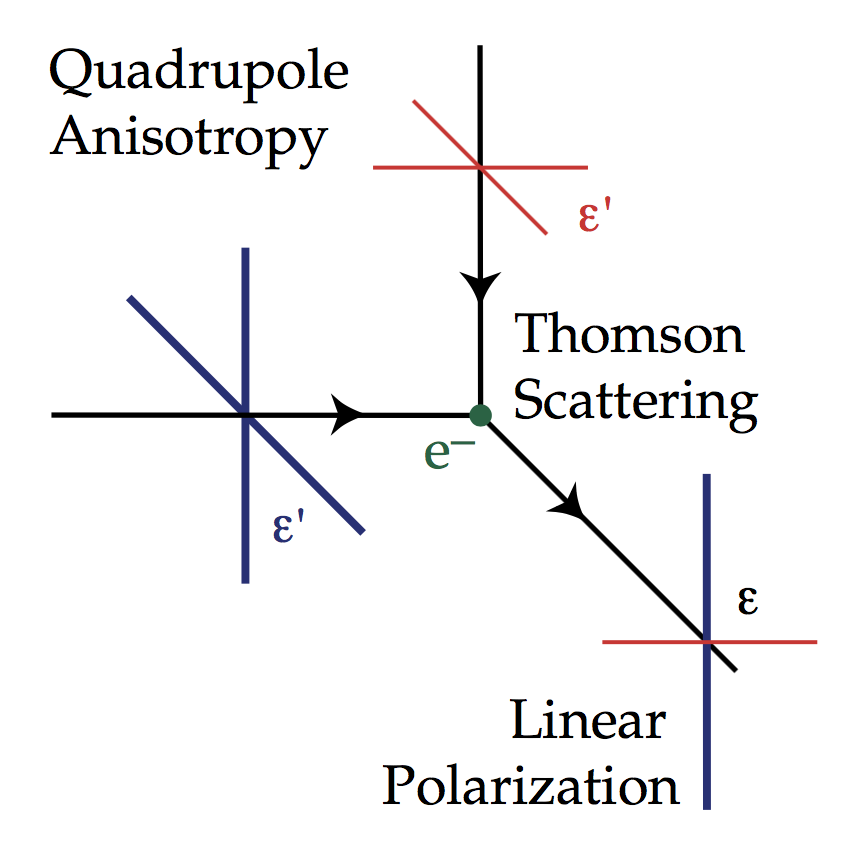
\includegraphics[width=12cm]{figures/ThomsonScattering.png}}
\end{figure}

{\noindent}If the incoming radiation field were isotropic, orthogonal polarization states from incident directions separated by $90^\circ$ would balance so that the outgoing radiation would remain unpolarized. Conversely, if the incident radiation field possesses a quadrupolar variation in intensity or temperature (which possess intensity peaks at $90^\circ=\pi/2$ separations), the result is a linear polarization of the scattered radiation (see Figure \ref{fig:Thomsonscattering}). A reversal in sign of the temperature fluctuation corresponds to a $90^\circ$ rotation of the polarization, which reflects the spin-$2$ nature of polarization.

{\noindent}In terms of a multipole decomposition of the radiation field into spherical harmonics, $Y_\ell^m(\theta,\phi)$, the five quadrupole moments are represented by $\ell= 2, m=O,\pm1,\pm2$. The orthogonality of the spherical harmonics guarantees that no other moment can generate polarization from Thomson scattering. In these spherical coordinates, with the north pole at $\theta=0$, we call a N-S (E-W) polarization component $Q>0$ ($Q<0$) and a NE-SW (NW-SE) component $U>0$ ($U<0$). The polarization amplitude and angle clockwise from north are

\begin{align*}
    P = \sqrt{Q^2+U^2}
\end{align*}

{\noindent}and

\begin{align*}
    \chi = \frac{1}{2}\arctan\left(\frac{U}{Q}\right).
\end{align*}

{\noindent}where $P$ is the polarized intensity and $Q$ and $U$ are the linear polarization Stokes vectors.

{\noindent}If Thomson scattering is rapid, then the randomization of photon directions that results destroys any quadrupole anisotropy and polarization. The problem of understanding the polarization pattern of the CMB thus reduces to understanding the quadrupolar temperature fluctuations at last scattering. Temperature perturbations have 3 geometrically distinct sources: the scalar (compressional), vector (vertical) and tensor (gravitational wave) perturbations. Formally, they form the irreducible basis of the symmetric metric tensor. We shall consider each of these below and show that the scalar, vector, and tensor quadrupole anisotropy correspond to $m=0,\pm1,\pm2$ respectively. This leads to different patterns of polarization for the three sources.

\subsubsection{Follow-up Questions}

\begin{itemize}
    \item What are some foregrounds or challenges to observing this signal?
    \item Why does dust polarize the CMB?
    \item Why is dust not randomly oriented?
    \item How did we first determine that dust is not randomly oriented?
\end{itemize}

% --------------------------------------------------------------
%
%                           10. 
%
% --------------------------------------------------------------

\newpage
\subsection{Question 10}

Our view of the cosmic microwave background is affected by what is along the line of sight. Give two examples of CMB foregrounds that also provide information about the cosmic parameters.

\subsubsection{Short answer}

Short answer.

\subsubsection{Additional context}

{\noindent}\textbf{The thermal Sunyaev-Zeldovich effect}: 

{\noindent}Given that the amplitude of the polarization is so small the question of foregrounds is even more important than for the temperature anisotropy. Unfortunately, the level and structure of the various foreground polarization in the CMB frequency bands is currently not well known. Atmospheric emission is believed to be negligibly polarized, leaving the main astrophysical foregrounds: free-free, synchrotron, dust, and point source emissions. Of these the most important foreground is synchrotron emission.

{\noindent}Free-free emission (bremsstrahlung) is intrinsically unpolarized but can be partially polarized by Thomson scattering within the HII region. This small effect is not expected to polarize the emission by more than 10\%. The emission is larger at low frequencies but is not expected to dominate the polarization at any frequency.

{\noindent}The polarization of dust is not well known. In principle, emission from dust particles could be highly polarized, however it's been found that that the majority of dust is polarized at the $\approx2\%$ level at $100\mu{\rm m}$ with a small fraction of regions approaching 10\% polarization. It's also been shown that even at 100\% polarization, extrapolation of the IRAS $100\mu{\rm m}$ map with the COBE FIRAS index shows that dust emission is negligible below $80\,{\rm GHz}$. At higher frequencies it will become the dominant foreground.

{\noindent}Radio point sources are polarized due to synchrotron
emission at $<20\%$ level. For large angle experiments, the random contribution from point sources will contribute negligibly, but may be of more concern for the upcoming satellite missions.

{\noindent}Galactic synchrotron emission is the major concern. It is potentially highly polarized with the fraction dependent on the spectral index and depolarization from Faraday rotation and non-uniform magnetic fields. The level of polarization is expected to lie between 10\%-75\% of a total intensity which itself is approximately $5\,\mu{\rm K}$ at $30\,{\rm GHz}$. This estimate follows from extrapolating measurements at $1411\,{\rm MHz}$ with an index of $T\propto\nu^{-3}$.

{\noindent}Due to their different spectral indices, the minimum
in the foreground polarization, like the temperature, lies near $100\,{\rm GHz}$. For full sky measurements, since synchrotron emission is more highly polarized than dust, the optimum frequency at which to measure intrinsic (CMB) polarization is slightly higher than for the anisotropy. Over small regions of the sky where one or the other of the foregrounds is known a priori to be absent the optimum frequency would clearly be different. However as with anisotropy measurements, with multi-frequency coverage, polarized foregrounds can be
removed.

{\noindent}It is also interesting to consider whether the spatial as well as frequency signature of the polarization can be used to separate foregrounds. Using angular power spectra for the spatial properties of the foregrounds is a simple generalization of methods already used in anisotropy work. For instance, in the case of synchrotron emission, if the spatial correlation in the polarization follows that of the temperature itself, the relative contamination will decrease on smaller angular scales due to its diffuse nature. Furthermore the peak of the cosmic signal in polarization occurs at even smaller angular scales than for the anisotropy.

{\noindent}Of those that can provide information about the cosmic parameters...

{\noindent}\textbf{The thermal Sunyaev–Zeldovich effect}: Electrons in the hot gas of the intracluster medium (ICM) can inverse Compton scatter photons of the CMB. The optical depth and thus the scattering probability for this inverse Compton scattering is relatively low, but the effect is nevertheless observable and, in addition, is of great importance for the analysis of clusters. A photon moving through a cluster of galaxies towards us will change its direction through scattering and thus will not reach us. But since the cosmic background radiation is isotropic, for any CMB photon that is scattered out of the line-of-sight, another photon exists -- statistically -- that is scattered into it, so that the total number of photons reaching us is preserved. However, the energy of the photons changes slightly through scattering by the hot electrons, in a way that they have an (on average) higher frequency after scattering. Hence, by this inverse Compton scattering, energy is on average transferred from the electrons to the photons, as can be seen in Figure \ref{fig:szeffect}.

\begin{figure}[h]
    \floatbox[{\capbeside\thisfloatsetup{capbesideposition={right,top},capbesidewidth=4cm}}]{figure}[\FBwidth]
    {\caption{\footnotesize{The influence of the Sunyaev–Zeldovich effect on the cosmic background radiation. The dashed curve represents the Planck distribution of the unperturbed CMB spectrum, the solid curve shows the spectrum after the radiation has passed through a cloud of hot electrons. The magnitude of this effect, for clarity, has been very much exaggerated in this sketch. Source: Carlstrom et al. 2002, ARA\&A 40, 643. Image taken from Schneider (2006).}}
    \label{fig:szeffect}}
    {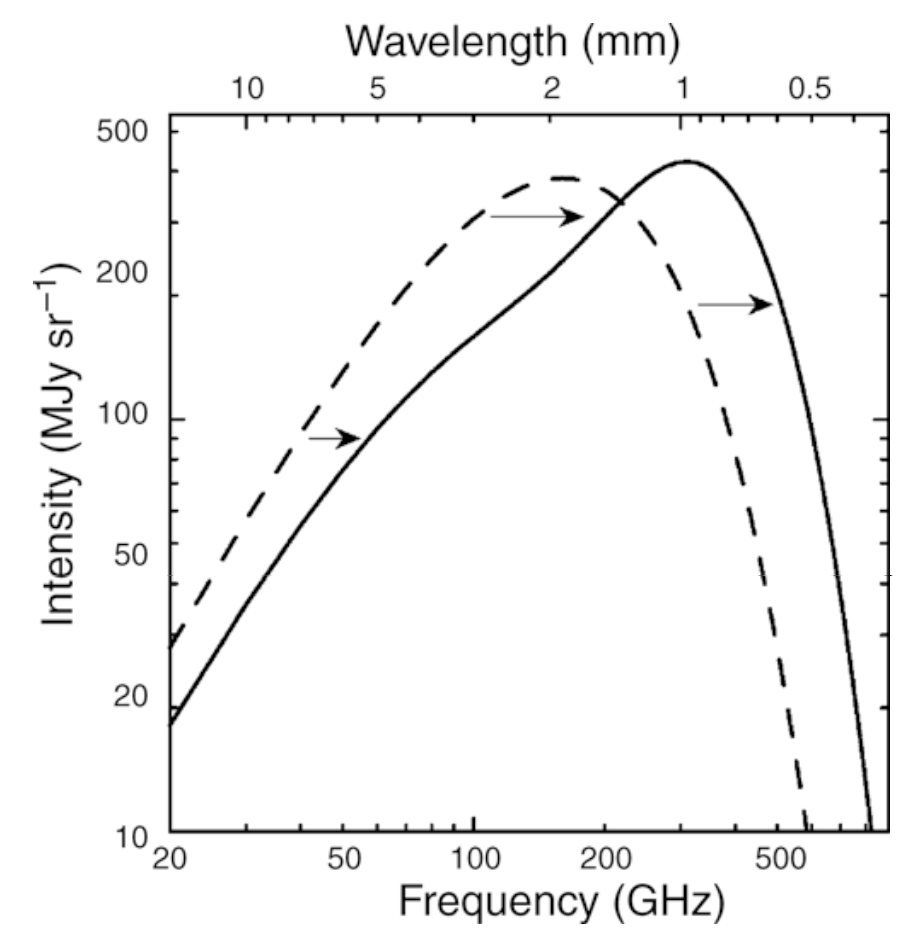
\includegraphics[width=8cm]{figures/SZeffect.png}}
\end{figure}

{\noindent}In the Rayleigh–Jeans (RJ) domain of the CMB spectrum, at wavelengths larger than about $2{\rm mm}$, the intensity of the CMB is decreased by the SZ-effect. For the change in specific intensity in the RJ part, one obtains

\begin{align*}
    \frac{\Delta I_\nu^\mathrm{RJ}}{I_\nu^\mathrm{RJ}} = -2y,
\end{align*}

{\noindent}where y is the the Compton parameter

\begin{align*}
    y = \int\frac{k_BT}{m_ec^2}\sigma_Tn_e\mathrm{d}l
\end{align*}

{\noindent}and $\sigma_T$ is the Compton cross-section for electron scattering

\begin{align*}
    \sigma_T = \frac{8\pi}{3}\left(\frac{e^2}{m_ec^2}\right)^2 = \frac{8\pi}{3}e_{e,0}^2.
\end{align*}

{\noindent}Obviously, $y$ is proportional to the optical depth with respect to Compton scattering, given as an integral over $n_e\sigma_T$ along the line-of-sight. Furthermore, $y$ is proportional to the gas temperature, because that defines the average energy transfer per scattering event. Overall, $y$ is proportional to the integral over the gas pressure $P D=nk_BT$ along the line-of-sight through the cluster.

{\noindent}The SZ effect affects the temperature distribution of the CMB. Some of the photons propagating along lines-of-sight passing through clusters of galaxies or other regions of dense and hot gas are scattered by the hot electrons, resulting in a temperature change in these directions. We recall that in the direction of clusters the measured intensity of the CMB radiation is reduced at low frequencies, whereas it is increased at high frequencies. Hence, the SZ effect can be identified in the CMB data if measurements are conducted over a sufficiently large frequency range.


% --------------------------------------------------------------
%
%                           11. 
%
% --------------------------------------------------------------

\newpage
\subsection{Question 11}

Describe cosmological inflation. List at least three important observations it is intended to explain.

\subsubsection{Short answer}

Inflation can most generally be defined as a period of exponential expansion of the form

\begin{align*}
    a(t) \propto e^{Ht} ~ [{\rm dimensionless}]
\end{align*}

{\noindent}very early on in the Universe. Inflation is intended to explain the (1) horizon problem, (2) flatness problem, and (3) magnetic monopole problem. The flatness problem can be summarized by the statement, ``The universe is nearly flat today, and was even flatter in the past.'' The horizon problem can be summarized by the statement, ``The universe is nearly isotropic and homogeneous today, and was even more so in the past.'' The monopole problem can be summarized by the statement, ``The universe is apparently free of magnetic monopoles'' Inflation explains these puzzling aspects of our Universe, by flattening it, ensuring its homogeneity over large scales, and driving down the number density of magnetic monopoles which it contains. At present, there is not a consensus among cosmologists about the exact mechanism driving inflation.

\subsubsection{Additional context}

In the inflationary scenario it is presumed that at very
early times the vacuum energy density was much higher
than today, so that it dominated the Hubble expansion. Then $\dot{a}/a\approx\sqrt{\Lambda/3}$. This implies an exponential expansion of the Universe,

\begin{align*}
    a(t) \propto e^{Ht} ~ [{\rm dimensionless}]
\end{align*}

{\noindent}Obviously, this exponential expansion (or inflationary phase) cannot last forever. We assume that a phase transition took place in which the vacuum energy density is transformed into normal matter and radiation (a process called reheating), which ends the exponential expansion and after which the normal Friedmann evolution of the Universe begins.

{\noindent}At present, there is not a consensus among cosmologists about the exact mechanism driving inflation; there is no known scalar field which can drive inflation. (A skeptic might point out that there is no known fundamental scalar held at all!) Therefore, it may well be true that the idea of inflation is correct but it is driven by something other than a scalar field. Having said that, there are a number of reasons to work with scalar fields, as we will do whenever we need to specify the source of inflation. Almost all fundamental particle physics theories contain scalar fields. In fact, historically it was particle physicists studying high-energy extensions of the Standard Model (in particular GUTs) who proposed the idea of inflation driven by a scalar field as a natural byproduct of some of these extensions. Indeed, almost all current work on inflation is based on a scalar field (or sometimes two). The alternative from a particle physics point of view is to use a vector field (such as the electromagnetic potential) or a set of fermions (similar to the way condensates induce superconductivity) to drive inflation. Neither of these choices works very well, but they both complicate things severely, so we will stick to a scalar field.

\begin{figure}[h]
    \floatbox[{\capbeside\thisfloatsetup{capbesideposition={right,top},capbesidewidth=4cm}}]{figure}[\FBwidth]
    {\caption{\footnotesize{During an inflationary phase, indicated here by the gray bar, the universe expands exponentially; see (4.83). This phase comes to an end when a phase transition transforms the vacuum energy into matter and radiation, after which the universe follows the normal Friedmann expansion. Adapted from: Alan Guth 1998, The inflationary Universe, Basic Books. Figure taken from Schneider (2006).}}
    \label{fig:inflation}}
    {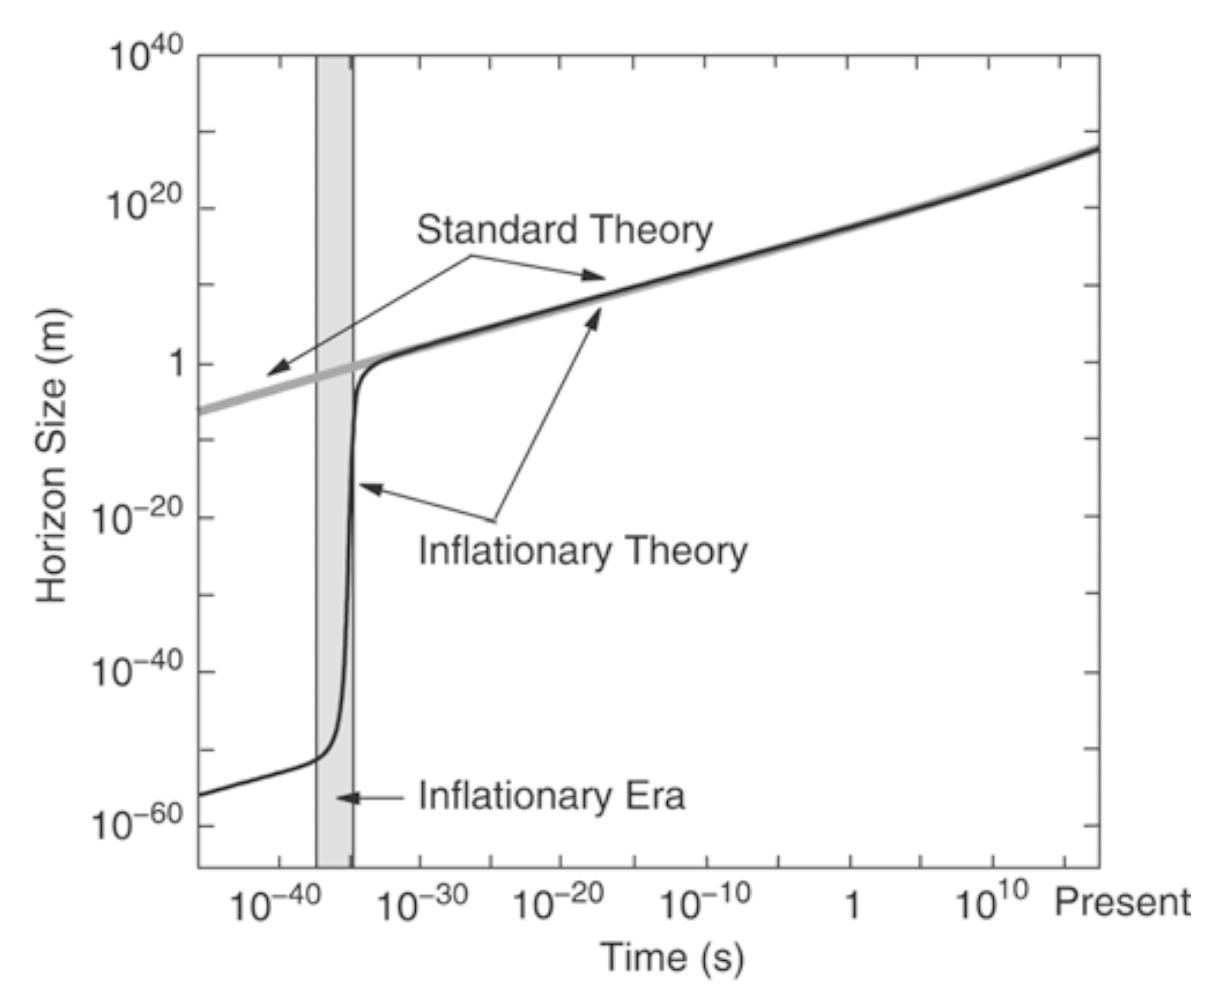
\includegraphics[width=12cm]{figures/Inflation.png}}
\end{figure}

{\noindent}\textbf{The horizon problem}: Since no signal can travel faster than light, the existence of a horizon length means that CMB radiation from two directions separated by more than about one degree originates in regions that were not in causal contact before recombination, (i.e., the time when the CMB photons interacted with matter the last time). Therefore, these two regions have never been able to exchange information, for example about their temperature. Nevertheless their temperature is the same, as seen from the high degree of isotropy of the CMB, which shows relative fluctuations of only $\Delta T/T10^{-5}$!

{\noindent}During inflation, $H(a)=\sqrt{\Lambda/3}$ is constant so that the integral for the comoving horizon length formally diverges. This implies that the horizon may become arbitrarily large in the inflationary phase, depending on the duration of the exponential expansion. For illustration we consider a very small region in space of size $L<ct_i$ at a time $t_i\sim10^{-34}\,{\rm s}$ prior to inflation which is in causal contact. Through inflation, it expands tremendously, e.g., by a factor $10^{40}$; the original $L\sim10^{-24}\,{\rm cm}$ inflates to about $10^{16}\,{\rm cm}$ by the end of the inflationary phase, at $t_f\sim10^{-32}{\rm s}$. By today, this spatial region will have expanded by another factor of $10^{25}$ by following (for $t>t_f$) the normal cosmic expansion, to   $10^{41}\,{\rm cm}$. This scale is considerably larger than the size of the currently visible Universe, $c/H_0$. According to this scenario, the whole Universe visible today was in causal contact prior to inflation, so that the homogeneity of the physical conditions at recombination, and with it the nearly perfect isotropy of the CMB, is provided by causal processes.

{\noindent}\textbf{The flatness problem}: For the total density parameter to be of order unity today, it must have been extremely close to $1$ at earlier times, which means that a very precise `fine tuning' of this parameter was necessary.

{\noindent}\textbf{The monopole problem}: The monopole problem -- that is, the apparent lack of magnetic monopoles in the Universe -- is not a purely cosmological problem, but one that results from combining the Hot Big Bang scenario with the particle physics concept of a Grand Unified Theory. In particle physics, a Grand Unified Theory, or GUT, is a field theory which attempts to unify the electromagnetic force, the weak nuclear force, and the strong nuclear force. Unification of forces has been a goal of scientists since the 1870s, when James Clerk Maxwell demonstrated that electricity and magnetism are both manifestations of a single underlying electromagnetic field. Currently, it is customary to speak of the four fundamental forces of nature: gravitational, electromagnetic, weak, and strong. In the view of many physicists, though, four forces are three too many; they've spent much time and effort to show that two or more of the ``fundamental forces'' are actually different aspects of a single underlying force. About a century after Maxwell, Steven Weinberg, Abdus Salam, and Sheldon Glashow successfully devised an electroweak theory. They demonstrated that at particle energies greater than $E\sim1\,{\rm TeV}$, the electromagnetic force and the weak force unite to form a single ``electroweak'' force. The electroweak energy of $E_\mathrm{ew}\sim1\,{\rm TeV}$ corresponds to a temperature $T_\mathrm{ew}\sim E_\mathrm{ew}/k_B\sim10^{16}\,{\rm K}$; the Universe had this temperature when its age was $t_\mathrm{ew}\sim10^{-12}\,{\rm s}$. Thus, when the Universe was less than a picosecond old, there were only three fundamental forces: the gravitational, strong, and electroweak force. When the predictions of the electroweak energy were confirmed experimentally, Weinberg, Salam, and Glashow toted home their Nobel Prizes, and physicists braced themselves for the next step: unifying the electroweak force with the strong force.

{\noindent}By extrapolating the known properties of the strong and electroweak forces to higher particle energies, physicists estimate that at an energy $E_\mathrm{GUT}$ of roughly $10^{12}-10^{13}\,{\rm TeV}$, the strong and electroweak forces should be unified as a single Grand Unified Force. If the GUT energy is $E_\mathrm{GUT}\sim10^{12}\,{\rm TeV}$, this corresponds to a temperature $T_\mathrm{GUT}\sim10^{28}\,{\rm K}$ and an age for the universe of $t_\mathrm{GUT}\sim10^{-36}\,{\rm s}$. The GUT energy is about four orders of magnitude smaller than the Planck energy, $E_\mathrm{P}\sim10^{16}\,{\rm TeV}$. Physicists are searching for a Theory of Everything (TOE) which describes how the Grand Unified Force and the force of gravity ultimately unite to form a single unified force at the Planck scale. The different unification energy scales, and the corresponding temperatures and times in the early Universe, are shown in Figure \ref{fig:gut}.

\begin{figure}[h]
    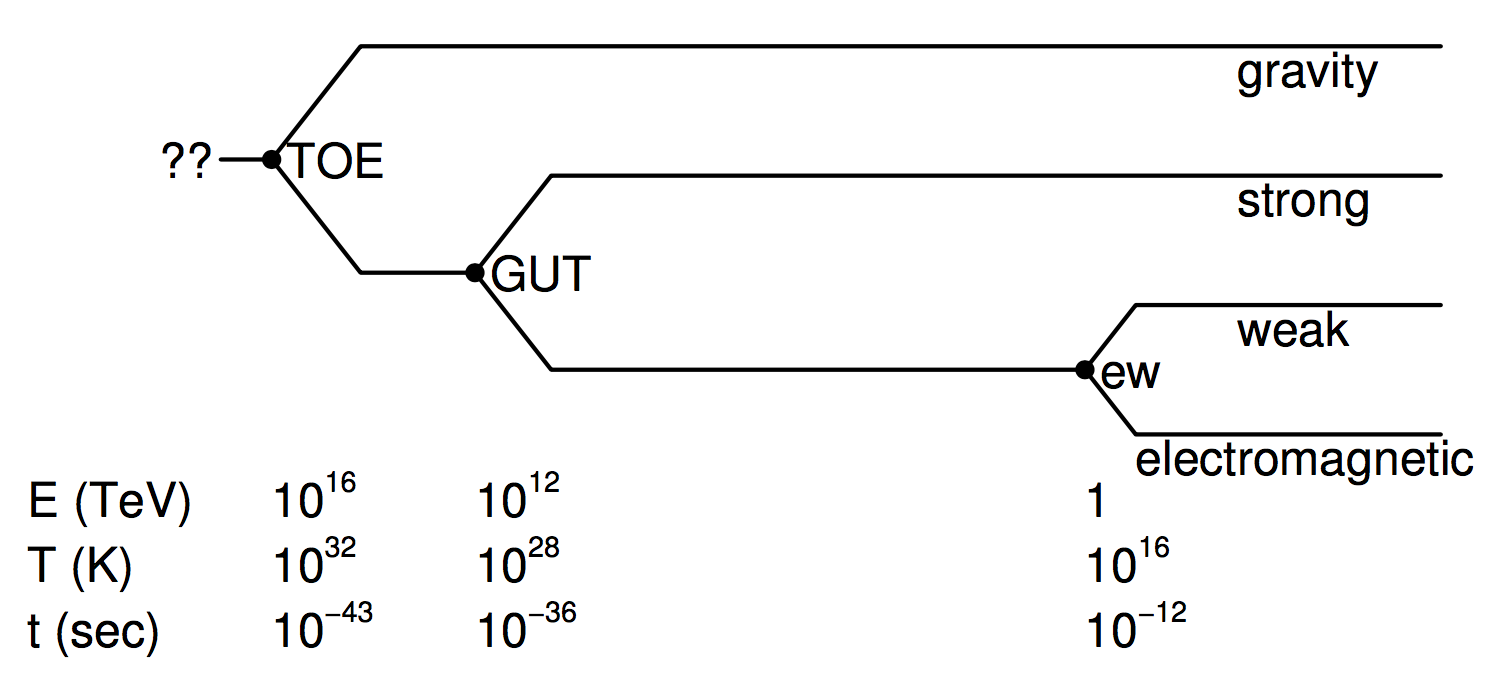
\includegraphics[width=16cm]{figures/GUT.png}
    \centering
    \caption{\footnotesize{The energy, temperature, and time scales at which the different force unifications occur. Image taken from Ryden (2006).}}
    \label{fig:gut}
\end{figure}

{\noindent}One of the predictions of GUT is that the Universe underwent a phase transition as the temperature dropped below the GUT temperature. Generally speaking, phase transitions are associated with a spontaneous loss of symmetry as the temperature of a system is lowered. Take, as an example, the phase transition known as ``freezing water''. At temperatures $T>273\,{\rm K}$, water is liquid. Individual water molecules are randomly oriented, and the liquid water thus has rotational symmetry about any point; in other words, it is isotropic. However, when the temperature drops below $T=273\,{\rm K}$, the water undergoes a phase transition, from liquid to solid, and the rotational symmetry of the water is lost. The water molecules are locked into a crystalline structure, and the ice no longer has rotational symmetry about an arbitrary point. In other words, the ice crystal is anisotropic, with preferred directions corresponding to the crystal’s axes of symmetry. In a broadly similar vein, there is a loss of symmetry when the universe undergoes the GUT phase transition at $t_\mathrm{GUT}\sim10^{-36}\,{\rm s}$. At $T>T_\mathrm{GUT}$, there was a symmetry between the strong and electroweak forces. At $T<T_\mathrm{GUT}$, the symmetry is spontaneously lost; the strong and electroweak forces begin to behave quite differently from each other.

{\noindent}In general, phase transitions associated with a loss of symmetry give rise to flaws known as topological defects. To see how topological defects form, consider a large tub of water which is cooled below $T=273\,{\rm K}$. Usually, the freezing of the water will start at two or more widely separated nucleation sites. The crystal which forms about any given nucleation site is very regular, with well-defined axes of symmetry. However, the axes of symmetry of two adjacent ice crystals will be misaligned. At the boundary of two adjacent crystals, there will be a two-dimensional topological defect, called a domain wall, where the axes of symmetry fail to line up. Other types of phase transitions give rise to one-dimensional, or line-like, topological defects (in a cosmological context, these linear defects are known as cosmic strings). Still other types of phase transitions give rise to zero-dimensional, or point-like, topological defects. GUT predict that the GUT phase transition creates point-like topological defects which act as magnetic monopoles. That is, they act as the isolated north pole or south pole of a magnet. The rest energy of the magnetic monopoles created in the GUT phase transition is predicted to be $m_Mc^2\sim E_\mathrm{GUT}\sim10^{12}\,{\rm TeV}$. This corresponds to a mass of over a nanogram (comparable to that of a bacterium), which is a lot of mass for a single particle to be carrying around. At the time of the GUT phase transition, points further apart than the horizon size will be out of causal contact with each other. Thus, we expect roughly one topological defect per horizon volume, due to the mismatch of fields which are not causally linked. The number density of magnetic monopoles, at the time of their creation, would be

\begin{align*}
    n_M(t_\mathrm{GUT}) \sim \frac{1}{(2ct_\mathrm{GUT})^3} \sim 10^{82} ~ [{\rm m^{-3}}],
\end{align*}

{\noindent}and their energy density would be

\begin{align*}
    (m_Mc^2)n_M \sim 10^{94}\,{[\rm TeV\,m^{-3}]}.
\end{align*}

{\noindent}This is a large energy density, but it is smaller by ten orders of magnitude than the energy density of radiation at the time of the GUT phase transition:

\begin{align*}
    \alpha T_\mathrm{GUT}^4 \sim 10^{104}\,{[\rm TeV\,m^{-3}]}.
\end{align*}

{\noindent}Thus, the magnetic monopoles wouldn't have kept the Universe from being radiation-dominated at the time of the GUT phase transition. However, the magnetic monopoles, being so massive, would soon have become highly non-relativistic, with energy density $\propto a^{-3}$. The energy density in radiation, though, was falling off at the rate $\propto a^{-4}$. Thus, the magnetic monopoles would have dominated the energy density of the Universe when the scale factor had grown by a factor $\sim10^{10}$; that is, when the temperature had fallen to $T\sim10^{-10}\,T_\mathrm{GUT}\sim10^{18}\,{\rm K}$, and the age of the universe was only $t\sim10^{-16}\,{\rm s}$.

{\noindent}Obviously, the Universe is not dominated by magnetic monopoles today. In fact, there is no strong evidence that they exist at all. Every north magnetic pole which we can find is paired with a south magnetic pole, and vice versa. There are no isolated north poles or isolated south poles. The monopole problem can thus be rephrased as the question, ``Where have all the magnetic monopoles gone?'' Now, you can always answer the question, ``Where have the monopoles gone?'' by saying, ``There were never any monopoles to begin with''” There is not yet a single, definitive GUT, and in some variants on the GUT theme, magnetic monopoles are not produced. However, the flatness and horizon problems are not so readily dismissed. When the physicist Alan Guth first proposed the idea of inflation in 1981, he introduced it as a way of resolving the flatness problem, the horizon problem, and the monopole problem with a single cosmological mechanism.

\subsubsection{Follow-up Questions}

\begin{itemize}
    \item Can you calculate/give an estimate or back-of-the-envelope idea of how flat the universe would have been after inflation if today it was say 1\% non-flat?
    \item What physically causes inflation?
    \item Why, physically, does having an inflaton result in inflation? What physically happens?

\end{itemize}

% --------------------------------------------------------------
%
%                           12. 
%
% --------------------------------------------------------------

\newpage
\subsection{Question 12}

Define and describe a 'fine tuning problem'. How do anthropic arguments attempt to resolve it?

\subsubsection{Short answer}

Answer.

\subsubsection{Additional context}

Additional context.

\subsubsection{Follow-up Questions}

\begin{itemize}
    \item What are other fine tuning problems? (Note: if you talk about $\Omega_k$, you cannot talk about $\Omega_\Lambda$ since they are related.)
    \item How do you \textit{feel} about the anthropic principle?
\end{itemize}


% --------------------------------------------------------------
%
%                           13. 
%
% --------------------------------------------------------------

\newpage
\subsection{Question 13}

Define the two-point correlation function. How is it related to the power spectrum? How is the $C_\ell$ spectrum of the CMB related to low redshift galaxy clustering?

\subsubsection{Short answer}

Answer.

\subsubsection{Additional context}

Since the CMB temperature fluctuations $\delta T/T$ is defined on the surface of a sphere -- the celestial sphere, in this case -- it is useful to expand it in spherical harmonics:

\begin{align*}
    \frac{\delta T}{T}(\theta,\phi) = \sum\limits_{\ell=0}^{\infty}\sum\limits_{m=-1}^{\ell} a_{\ell m}Y_{\ell m}(\theta,\phi)
\end{align*}

{\noindent}where $Y_{\ell m}(\theta,\phi)$ are the usual spherical harmonic functions\footnote{\href{https://en.wikipedia.org/wiki/Table\_of\_spherical\_harmonics}{https://en.wikipedia.org/wiki/Table\_of\_spherical\_harmonics}}. What concerns cosmologists is not the exact pattern of hot spots and cold spots on the sky, but their statistical properties. The most important statistical property of $\delta T/T$ is the correlation function $C(\theta)$. Consider two points on the last scattering surface. Relative to an observer, they are in the directions $\hat{n}$ and $\hat{n}'$, and are separated by an angle $\theta$ given by the relation $cos\theta=\hat{n}\cdot\hat{n}'$. To find the correlation function $C(\theta)$, multiply together the values of $\delta T/T$ at the two points, then average the product over all points separated by the angle $\theta$:

\begin{align*}
    C(\theta) = \left\langle\frac{\delta T}{T}(\hat{n})\frac{\delta T}{T}(\hat{n}')\right\rangle_{\hat{n}\cdot\hat{n}'=\cos\theta}
\end{align*}

{\noindent}If cosmologists knew the precise value of $C(\theta)$ for all angles from $\theta=0$ to $\theta=180^\circ$, they would have a complete statistical description of the temperature fluctuations over all angular scales. Unfortunately, the CMB measurements which tell us about $C(\theta)$ contain information over only a limited range of angular scales.

{\noindent}The limited angular resolution of available observations is what makes the spherical harmonic expansion of $\delta T/T$ so useful. Using the expansion of $\delta T/T$ in spherical harmonics, the correlation function can be written in the form

\begin{align*}
    C(\theta) = \frac{1}{4\pi} \sum\limits_{\ell=0}^\infty (2\ell+\ell)(C_\ell)P_\ell(cos\theta),
\end{align*}

{\noindent}where $P_\ell$ are the usual Legendre polynomials:

\begin{align*}
    P_0(x) = 1 \\
    P_1(x) = x \\
    P_2(x) = \frac{1}{2}(3x^2-1)
\end{align*}

{\noindent}and so forth. In this way, a measured correlation function $C(\theta)$ can be broken down into its multipole moments $C_\ell$.

{\noindent}Generally speaking, a term $C_\ell$ is a measure of temperature fluctuations on the angular scale $\theta\sim180^\circ/\ell$. Thus, the multipole $\ell$ is interchangeable, for all practical purposes, with the angular scale $\theta$. The $\ell=0$ (monopole) term of the correlation function vanishes if you've defined the mean temperature correctly. The $\ell=1$ (dipole) term results primarily from the Doppler shift due to our motion through space. It is the moments with $\ell\geq2$ which are of the most interest to cosmologists, since they tell us about the fluctuations present at the time of last scattering.

{\noindent}In presenting the results of CMB observations, it is customary to plot the function

\begin{align*}
    \Delta T \equiv \sqrt{\frac{\ell(\ell+1)}{2\pi}}\langle T \rangle ~ [{\rm K}],
\end{align*}

{\noindent}since this function tells us the contribution per logarithmic interval in $\ell$ to the total temperature fluctuation $\delta T$ of the CMB. The detailed shape of the $\Delta T$ versus $\ell$ curve contains a wealth of information about the Universe at the time of photon decoupling. 

{\noindent}At the time of last scattering, a particularly interesting length scale, cosmologically speaking, is the Hubble distance,

\begin{align*}
    d_H = \frac{c}{H(z_\mathrm{ls})} \approx \frac{3\times10^8\,{\rm m\,s^{-1}}}{1.24\times10^{-18}\,s^{-1}(1101)^{3/2}} \approx 6.6\times10^{21}\,{\rm m} \approx 0.2\,{[\rm Mpc]},
\end{align*}

{\noindent}where the redshift of last scattering is $z_\mathrm{ls}\approx1100$. A patch of the last scattering surface with this physical size will have an angular size, as seen from Earth, of

\begin{align*}
    \theta_H = \frac{c/H(z_\mathrm{ls})}{d_A} \approx \frac{0.2\,{\rm Mpc}}{13\,{\rm Mpc}} \approx 0.015\,{\rm rad} \approx 1^\circ.
\end{align*}

{\noindent}It is no coincidence that the peak in the $\Delta T$ versus $\ell$ curve occurs at an angular scale $θ\sim\theta_H$. The origin of temperature fluctuations with $\theta>\theta_H$ ($\ell<180$) is different from those with $\theta<\theta_H$ ($\ell>180$).


% --------------------------------------------------------------
%
%                           14. 
%
% --------------------------------------------------------------

\newpage
\subsection{Question 14}

Consider a cosmological model including a positive cosmological constant. Show that, in such a model, the expansion factor eventually expands at an exponential rate. Sketch the time dependence of the expansion factor in the currently favoured cosmological model.

\subsubsection{Short answer}

Answer.

\subsubsection{Additional context}

{\noindent}The Benchmark Model, is adopted as the best fit to the currently available observational data, is spatially flat, and contains radiation, matter, and a cosmological constant. The Hubble constant of the Benchmark Model is assumed to be $H_0=70\,{\rm km\,s^{-1}\,Mpc^{-1}}$. The radiation in the Benchmark Model consists of photons and neutrinos. The photons are assumed to be provided solely by a CMB with current temperature $T_0=2.725\,{\rm K}$ and density parameter $\Omega_{\gamma,0}=5.0\times10^{-5}$. The energy density of the CNB is theoretically calculated to be 68\% of that of the CMB, as long as neutrinos are relativistic. If a neutrino has a non-zero mass $m_\nu$, it defects from the ``radiation'' column to the ``matter'' column when the scale factor is $a\sim5\times10^{-4}\,{\rm eV}/(m_\nu c^2)$. The matter content of the Benchmark Model consists partly of baryonic matter (that is, matter composed of protons and neutrons, with associated electrons), and partly of nonbaryonic dark matter; the evidence indicates that most of the matter in the Universe is nonbaryonic dark matter. The baryonic material that we are familiar with from our everyday existence has a density parameter of $\Omega_{b,0}\approx0.04$ today. The density parameter of the nonbaryonic dark matter is roughly six times greater: $\Omega_{c,0}\approx0.26$. The bulk of the energy density in the Benchmark Model, however, is not provided by radiation or matter, but by a cosmological constant, with $\Omega_{\Lambda,0}=1-\Omega_{m,0}-\Omega_{r,0}\approx0.70$.

{\noindent}The Benchmark Model was first radiation-dominated, then matter-dominated, and is now entering into its lambda-dominated phase. Radiation gave way to matter at a scale factor $a_{rm}=\Omega_{r,0}/\Omega{m,0}=2.8\times10^{-4}$, corresponding to a time $t_{rm}=4.7\times10^4\,{\rm yr}$. Matter, in turn, gave way to the cosmological constant at $a_{m\Lambda}=(\Omega_{m,0}/\Omega_{\Lambda,0})^{1/3}$ corresponding to $t_{m\Lambda}=9.8\,{\rm Gyr}$. The current age of the Universe, in the Benchmark Model, is $t_0=13.5\,{\rm Gyr}$.

{\noindent}With $\Omega_{r,0}$, $\Omega_{m,0}$, and $\Omega_{\Lambda,0}$ known, the scale factor $a(t)$ can be computed numerically using the Friedmann equation, in the form of

\begin{align*}
    \left(\frac{H}{H_0}\right)^2 = \frac{\Omega_{r,0}}{a^4} + \frac{\Omega_{m,0}}{a^3} + \Omega_{\Lambda,0} + \frac{1-\Omega_0}{a^2}
\end{align*}

{\noindent}where $\Omega_0=\Omega_{r,0}+\Omega_{m,0}+\Omega_{\Lambda,0}$. Since $(H/H_0)^2=(\dot{a}/a)^2$, this can be written as

\begin{align*}
    \left(\frac{\dot{a}(t)}{a(t)}\right)^2 &= \frac{\Omega_{r,0}}{a^4} + \frac{\Omega_{m,0}}{a^3} + \Omega_{\Lambda,0} + \frac{1-\Omega_0}{a^2} \\
    \dot{a}(t) &= a(t)\sqrt{\frac{\Omega_{r,0}}{a^4} + \frac{\Omega_{m,0}}{a^3} + \Omega_{\Lambda,0} + \frac{1-\Omega_0}{a^2}}.
\end{align*}

{\noindent}For $a\gg1$, this simplifies to

\begin{align*}
    \frac{\mathrm{d}a}{\mathrm{d}t} &\approx a(t)\sqrt{\Omega_{\Lambda,0}} \\
    a(t) &\approx e^{\sqrt{\Omega_{\Lambda,0}}t}.
\end{align*}

{\noindent}Therefore, at large scale factors, the expansion proceeds at the exponential rate as follows:

\begin{align*}
    a(t) \propto e^{\sqrt{\Omega_{\Lambda,0}}t}.
\end{align*}

{\noindent}Figure \ref{fig:avst} shows the scale factor, thus computed, for the Benchmark Model. Note that the transition from the $a\propto t^{1/2}$ radiation-dominated phase to the $a\propto t^{2/3}$ matter-dominated phase is not an abrupt one; neither is the later transition from the matter-dominated phase to the exponentially growing lambda-dominated phase. One curious feature of the Benchmark Model which Figure \ref{fig:avst} illustrates vividly is that we are living very close to the time of matter-lambda equality.

\begin{figure}[t]
    \floatbox[{\capbeside\thisfloatsetup{capbesideposition={right,top},capbesidewidth=4cm}}]{figure}[\FBwidth]
    {\caption{\footnotesize{The scale factor $a$ as a function of time $t$ (measured in units of the Hubble time), computed for the Benchmark Model. The dotted lines indicate the time of radiation-matter equality, $a_{rm}=2.8\times10^{-4}$, the time of matter-lambda equality, $a{m\Lambda}=0.75$, and the present moment, $a_0=1$. Figure taken from Ryden (2006).}}
    \label{fig:avst}}
    {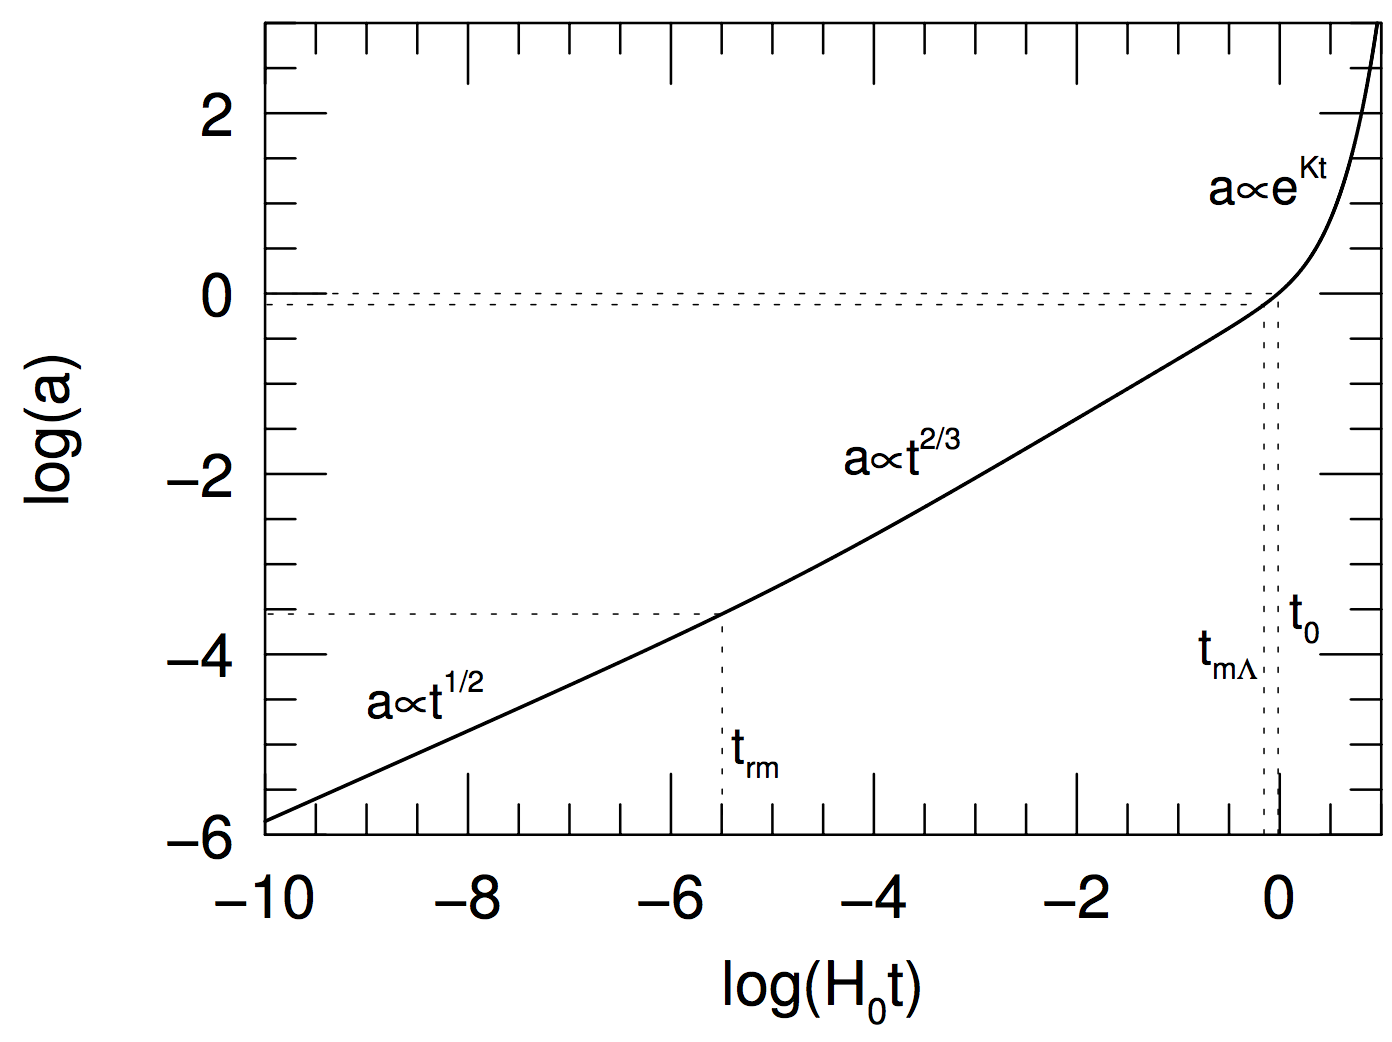
\includegraphics[width=12cm]{figures/avst.png}}
\end{figure}

% --------------------------------------------------------------
%
%                           15. 
%
% --------------------------------------------------------------

\newpage
\subsection{Question 15}

Define and describe the epoch of reionization. What are the observational constraints on it?

\subsubsection{Short answer}

After recombination occurring at a redshift $z\sim1,100$, the Universe entered the cosmic \textit{Dark Ages} where it became predominantly neutral until $z\sim16$. Around this time, gravitational Jeans instabilities allowed for the formation of the first generation of stars. While they have yet to be directly observed, these Population III (Pop III) stars were particular massive ($\sim100\,M_\odot$), implying that they were extremely hot and capable of radiating significant amounts of ionizing UV photons. These Pop III stars triggered a significant phase transition in the IGM as they began ionizing the predominantly neutral gas during a time called the \textit{Epoch of Reionization} (EoR). There are several observational constraints on this period, including Ly$\alpha$ forest lines, Gunn-Peterson absorption, and CMB polarization.


\subsubsection{Additional context}

{\noindent}The baryonic pre-galactic medium (PGM) evolves in three distinct phases. At high redshifts ($z>1100$) the PGM is hot, fully ionized, and optically thick to Thomson scattering, and hence coupled to the photon field. As the universe expands, the PGM cools, and eventually recombines, leaving a surface of last scattering (the CMB), plus a neutral PGM. This neutral phase lasts from $z=1100$ to $z\sim14$. At some point between $z\sim14$ and $6$, hydrogen in the PGM is ``reionized,'' due to UV radiation from the first luminous objects, leaving the fully reionized IGM seen during the ``realm of the galaxies'' ($0<z<6$). The ionized, dense PGM at very high redshift has been well studied through extensive observations of the CMB. Likewise, the reionized, rarified IGM at low redshift has been well characterized through QSO absorption line studies. The middle phase (the existence of a neutral IGM during the so-called dark ages and the process of reionization of this medium) is the last directly observable phase of cosmic evolution that remains to be verified and explored. The epoch of reionization (EoR) is crucial in cosmic structure formation studies, because it sets a fundamental benchmark indicating the formation of the first luminous objects, either star-forming galaxies or active galactic nuclei (AGN).

{\noindent}After recombination at $z\sim1100$, the intergalactic gas became neutral, with a residual ionization fraction of only $10^{-4}$. Had the Universe remained neutral we would not be able to receive any photons that were emitted bluewards of the Ly$\alpha$ line of a source, because the absorption cross section for Ly$\alpha$ photons is too large. Since such photons are observed from QSOs, as can be seen for instance in the spectra of the $z>5.7$ QSOs in Figure \ref{fig:qsoabsorption}, and since an appreciable fraction of homogeneously distributed neutral gas in the intergalactic medium can be excluded for $z\gtrsim5$, from the tight upper bounds on the strength of the Gunn-Peterson effect, the Universe must have been reionized between the recombination epoch and the redshift $z\sim7$ of the most distant known QSOs.

{\noindent}This raises the question of how this reionization proceeded, in particular which process was responsible for it. The latter question is easy to answer -- reionization must have happened by photoionization. Collisional ionization can be ruled out because for it to be efficient the intergalactic medium (IGM) would need to be very hot, a scenario which can be excluded due to the perfect Planck spectrum of the CMB. Hence, the next question is what produced the energetic photons that caused the photoionization of the IGM.

{\noindent}Two kinds of sources may in principle account for them -- hot stars or AGNs. Currently, it is not unambiguously clear which of these is the predominant source of energetic photons causing reionization since our current understanding of the formation of supermassive black holes is still insufficient. However, it is currently thought that the main source of photoionization photons is the first generation of hot stars.

{\noindent}Following on from the above arguments, understanding reionization is thus directly linked to studying the first generation of stars. In the present Universe star formation occurs in galaxies; thus, one needs to examine when the first galaxies could have formed. From the theory of structure formation, the mass spectrum of dark matter halos at a given redshift can be computed by means of, e.g., the Press-Schechter model. Two conditions need to be fulfilled for stars to form in these halos. First, gas needs to be able to fall into the dark halos. Since the gas has a finite temperature, pressure forces may impede the infall into the potential well. Second, this gas also needs to be able to cool, condensing into clouds in which stars can then be formed.

{\noindent}By means of a simple argument, we can estimate under which conditions pressure forces are unable to prevent the infall of gas into a potential well. To do this, we consider a slightly overdense spherical region of radius $R$ whose density is only a little larger than the mean cosmic matter density $\bar{\rho}$. If this sphere is homogeneously filled with baryons, the gravitational binding energy of the gas is about

\begin{align*}
    \lvert E_\mathrm{pot} \rvert \sim \frac{GMM_g}{R} ~ [{\rm J}],
\end{align*}

{\noindent}where $M$ and $M_g$ denote the total mass and the gas mass of the sphere, respectively. The thermal energy of the gas can be computed from the kinetic energy per particle, multiplied by the number of particles in the gas, or

\begin{align*}
    E_\mathrm{th} &\sim c_s^2M_g ~ [{\rm J}],    
\end{align*}

{\noindent}where the sound speed is given by

\begin{align*}
    c_s \approx \sqrt{\frac{k_BT}{\mu m}} ~ [{\rm m\,s^{-1}}]
\end{align*}

\begin{figure}[t]
    \floatbox[{\capbeside\thisfloatsetup{capbesideposition={right,top},capbesidewidth=4cm}}]{figure}[\FBwidth]
    {\caption{\footnotesize{\\Spectra of five QSOs at redshifts $z>5.7$, discovered in multi-color data from the Sloan Digital Sky Survey. The positions of the most important emission lines are marked. Particularly remarkable is the almost complete lack of flux bluewards of the Ly$\alpha$ emission line in some of the QSOs, indicating a strong Gunn-Peterson effect. However, this absorption is not complete in all QSOs, which points at strong variations in the density of neutral hydrogen in the IGM at these high redshifts. Either the hydrogen density varies strongly for different lines-of-sight, or the degree of ionization is very inhomogeneous. Source: X. Fan et al. 2004, A Survey of $z>5.7$ Quasars in the Sloan Digital Sky Survey. III. Discovery of Five Additional Quasars, AJ 128, 515, p. 517, Fig. 1. Figure taken from Ryden (2006).}}
    \label{fig:qsoabsorption}}
    {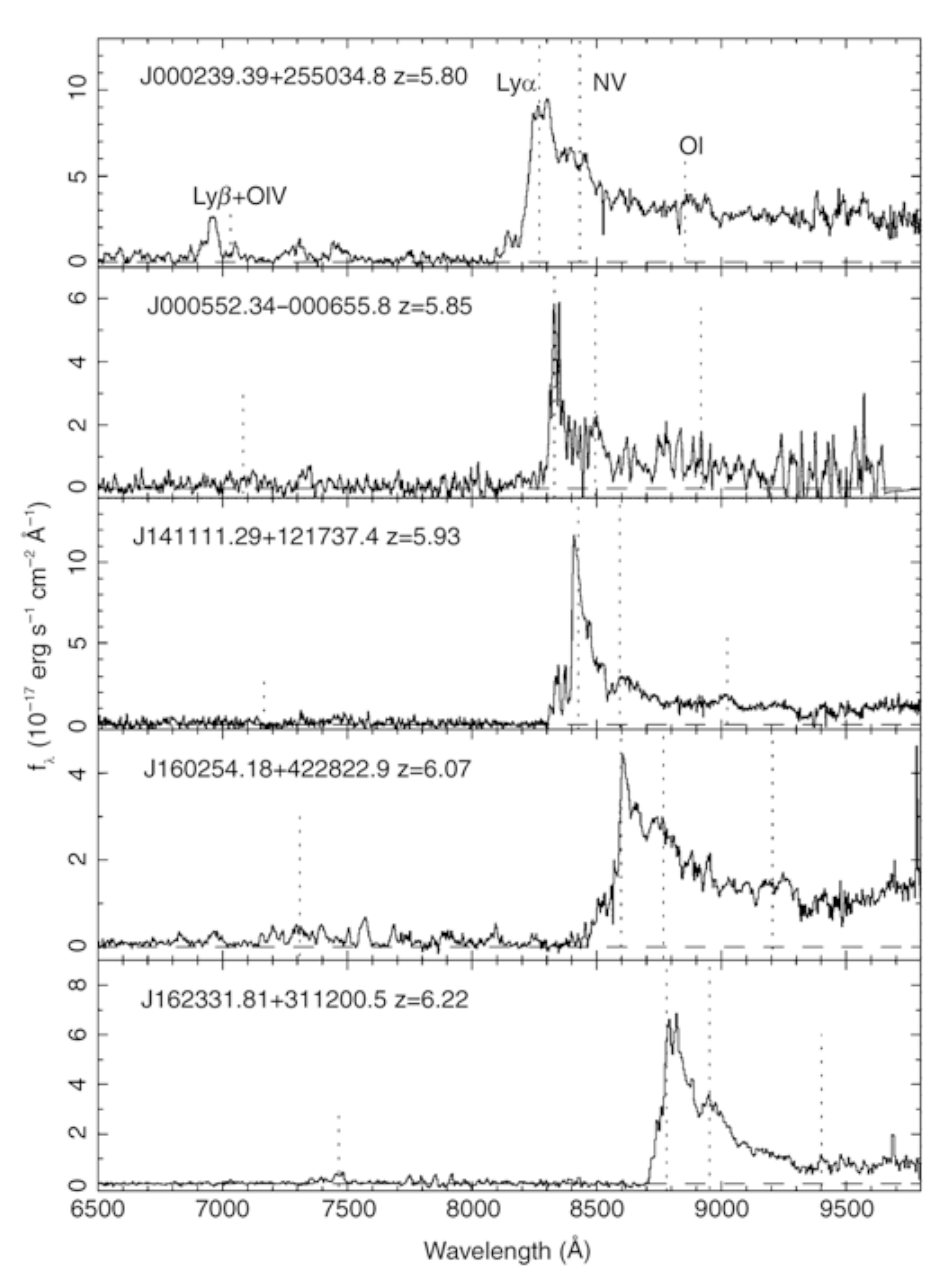
\includegraphics[width=9cm]{figures/QSOabsorption.png}}
\end{figure}

{\noindent}which is about the average velocity of the gas particles, and $m$ denotes the average particle mass in the gas. For the gas to be bound in the gravitational field, its gravitational binding energy needs to be larger than its thermal energy, $E_\mathrm{pot}>E_\mathrm{th}$, which yields the condition $GM>c_s^2R$. Since we have assumed an only slightly overdense region, the relation $M\sim\bar{\rho}R^3$ between mass and radius of the sphere applies. From the two latter equations, the radius can be eliminated, yielding the condition

\begin{align*}
    M > M_J \equiv \frac{\pi^{5/2}}{6}\left(\frac{c_s^2}{G}\right)^{3/2}\frac{1}{\sqrt{\bar{\rho}}} ~ [{\rm M_\odot}],
\end{align*}

{\noindent}where $M_J$ is the Jeans mass. The Jeans mass depends on the temperature of the gas, expressed through the sound speed $c_s$, and on the mean cosmic matter density $\bar{\rho}$. The latter can easily be expressed as a function of redshift, $\bar{\rho}(z) = \bar{\rho}_0(1+z)^3$.

{\noindent}The baryon temperature $T_b$ has a more complicated dependence on redshift. For sufficiently high redshifts, the small fraction of free electrons that remains after recombination provides a thermal coupling of the baryons to the cosmic background radiation, by means of Compton scattering. This is the case for redshifts $z>z_t$, where

\begin{align*}
    z_t \approx 140\left(\frac{\Omega_bh^2}{0.022}\right)^{2/5} ~ [{\rm dimensionless}]
\end{align*}

{\noindent}hence, $T_b(z)\approx T(z)=T_0(1+z)$ for $z>z_t$. For smaller redshifts, the density of photons gets too small to maintain this coupling, and baryons start to adiabatically cool down by the expansion, so that for $z\lesssim zt$ we obtain approximately $T_b\propto\rho_b^{2/3}\propto(1+z)^2$.

{\noindent}From these temperature dependencies, the Jeans mass then be calculated as a function of redshift. For $z_t\gtrsim z\gtrsim 1000$, $M_J$ is independent of $z$ because $c_s
\propto T^{1/2}\propto(1+z)^{1/2}$ and $\bar{\rho}\propto(1+z)^3$ and its value is

\begin{align*}
    M_J = 1.35\times10^5 \left(\frac{\Omega_mh^2}{0.15}\right)^{-1/2} ~ [{\rm M_\odot}],
\end{align*}

{\noindent}whereas for $z\gtrsim z_t$ we obtain, with $T_b\simeq1.7\times10^{-2}(1+z)^2\,{\rm K}$,

\begin{align*}
    M_J = 5.7\times10^3 \left(\frac{\Omega_mh^2}{0.15}\right)^{-1/2} \left(\frac{\Omega_bh^2}{0.022}\right)^{-3/5}\left(\frac{1+z}{10}\right)^{3/2} ~ [{\rm M_\odot}].
\end{align*}

{\noindent}Hence, gas can not fall into halos with mass lower than these values.

\begin{figure}[t]
    \floatbox[{\capbeside\thisfloatsetup{capbesideposition={right,top},capbesidewidth=4cm}}]{figure}[\FBwidth]
    {\caption{\footnotesize{The cooling function for gas with primordial composition (blue solid curve), 1/3 of the Solar metallicity (green dashed curve) and Solar metallicity (red dotted curve). On the top axis, the temperature is converted into a circular velocity. To obtain such a cooling function, one needs to assume an equilibrium state of the gas. Here it is assumed that the gas is in thermodynamical equilibrium, where the fraction of ionization states of any atom depends just on $T$ . The total cooling function shown here is a superposition of different gas cooling processes, including atomic processes and bremsstrahlung, the latter of which dominating at high $T$ where the gas is fully ionized. Source: C.M. Baugh 2006, A primer on hierarchical galaxy formation: the semi-analytical approach, arXiv:astro-ph/0610031, Fig.9. Figure taken from Ryden (2006).}}
    \label{fig:coolingfunction}}
    {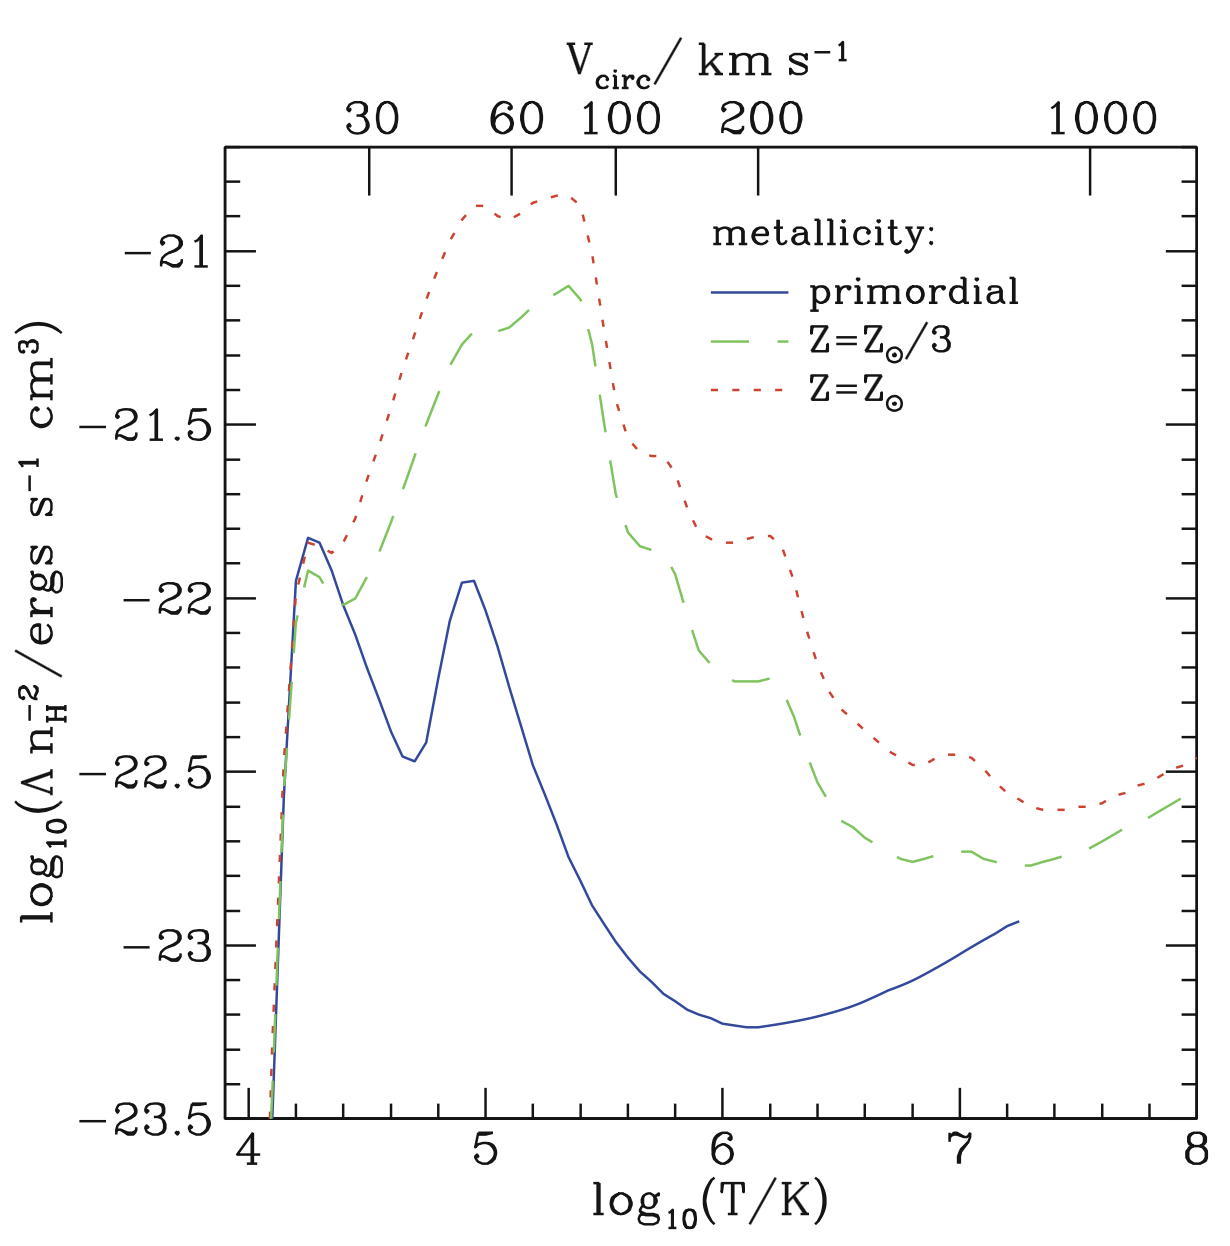
\includegraphics[width=10cm]{figures/CoolingFunction.png}}
\end{figure}

{\noindent}The Jeans criterion is a necessary condition for the formation of proto-galaxies (i.e., dark matter halos which contain baryons). In order to form stars, the gas in the halos needs to be able to cool further. Here, we are dealing with the particular situation of the first galaxies, whose gas is metal-free, so metal lines cannot contribute to the cooling. The cooling function of primordial gas is much smaller than that of enriched material; in particular, the absence of metals means that even slow cooling though excitation of fine-structure lines cannot occur, as there are no atoms with such transitions present. Thus, cooling by the primordial gas is efficient only above $T\gtrsim2\times10^4\,{\rm K}$. However, the halos formed at high redshift have low mass. The abundance of dark matter halos depends on the parameter $\nu$ which is the ratio between the density threshold required for collapse and the dispersion of fluctuations on a given mass scale. At high redshift, the growth factor $D_+(a)$ is small, and thus to have a noticeable abundance of halos of mass $M$, the dispersion $\sigma(M)$ must be correspondingly large. At redshift $z\sim10$, the parameter $\nu$ is about unity for halos of mass $\sim10^3\,{\rm M_\odot}$. Hence, at that time, substantially more massive halos than that were (exponentially) rare (i.e., only low-mass halos were around) and their virial temperature

\begin{align*}
    T_\mathrm{vir} \approx 2\times10^2 \left(\frac{M}{10^5h^{-1}\,{\rm M_\odot}}\right)^{2/3} \left(\frac{1+z}{10}\right) ~ [{\rm K}]
\end{align*}

{\noindent}is considerably below the energy scale where atomic hydrogen can efficiently cool. Here, we used the fact that the mean matter density of a halo inside its virial radius is   200 times the critical density at a given redshift. Therefore, atomic hydrogen is a very inefficient coolant for these first halos, insufficient to initiate the formation of stars. Furthermore, helium is of no help in this context, since its excitation temperature is even higher than that of hydrogen.

\begin{figure}[t]
    \floatbox[{\capbeside\thisfloatsetup{capbesideposition={right,top},capbesidewidth=4cm}}]{figure}[\FBwidth]
    {\caption{\footnotesize{Cooling rate as a function of the temperature for a gas consisting of atomic and molecular hydrogen (with 0.1\% abundance) and of helium. The solid curve describes the cooling by atomic gas, the dashed curve that by molecular hydrogen; thus, the latter is extremely important at temperatures below $\sim10^4\,{\rm K}$. At considerably lower temperatures the gas cannot cool, hence no star formation can take place. Source: R. Barkana \& A. Loeb 2000, In the Beginning: The First Sources of Light and the Reionization of the Universe, astro-ph/0010468, Fig. 12. Figure taken from Ryden (2006).}}
    \label{fig:coolingfunctionhydrogen}}
    {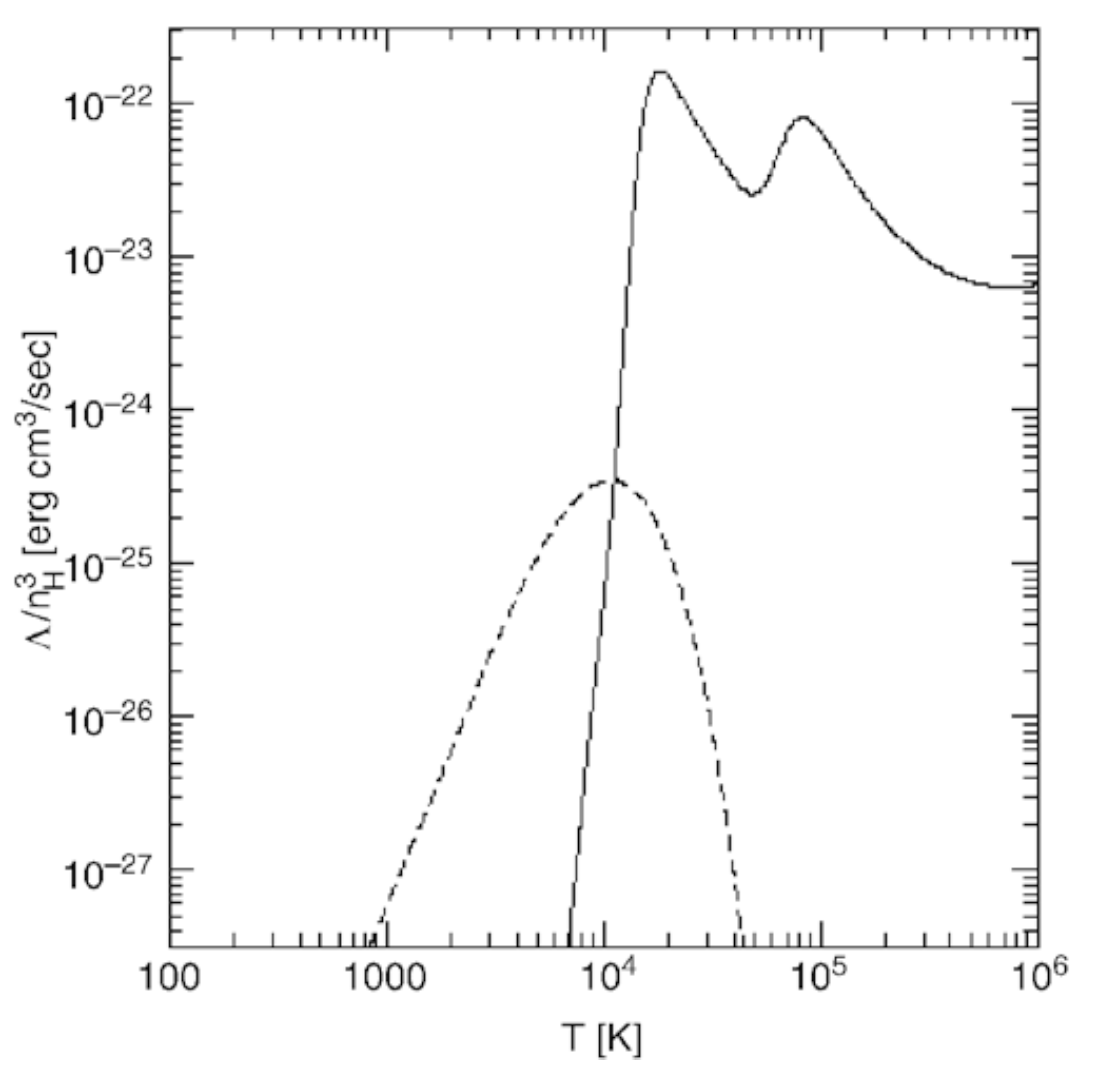
\includegraphics[width=10cm]{figures/CoolingFunctionHydrogen.png}}
\end{figure}

{\noindent}Besides atomic hydrogen and helium, the primordial gas contains a small fraction of molecular hydrogen which represents an extremely important component in cooling processes. Whereas in enriched gas, molecular hydrogen is formed on dust particles, the primordial gas had no dust, and so H$_2$ must form in the gas phase itself, rendering its abundance very small. However, despite its very small density and transition probability, H$_2$ dominates the cooling rate of primordial gas at temperatures below $T\sim10^4\,{\rm K}$ (see Figure \ref{fig:coolingfunctionhydrogen}) where the precise value of this temperature depends on the abundance of H$_2$.

{\noindent}By means of H$_2$, the gas can cool in halos with a temperature exceeding about $T_\mathrm{vir}\gtrsim1000\,{\rm K}$, corresponding to a halo mass of $M\gtrsim5\times10^4\,{\rm M_\odot}$ at $z\sim20$. In these halos, stars may then be able to form. These stars will certainly be different from those known to us, because they do not contain any metals. Therefore, the opacity of the stellar plasma is much lower. Such stars, which at the same mass presumably have a much higher temperature and luminosity (and thus a shorter lifetime), are called population III stars. Due to their high temperature they are much more efficient sources of ionizing photons than stars with `normal' metallicity.

{\noindent}The energetic photons from these population III stars are now capable of ionizing hydrogen in their vicinity. More important still is another effect: photons with energy above $11.26eV$ can destroy H$_2$. Since the Universe is transparent for photons with energies below $13.6\,{\rm eV}$, photons with $11.26\,{\rm eV}\geq E \geq 13.6\,{\rm eV}$ can propagate very long distances and dissociate molecular hydrogen. This means that as soon as the first stars have formed in a region of the Universe, molecular hydrogen in their vicinities will be destroyed and further gas cooling and star formation will then be prevented. At this point, the Universe contains a low number density of isolated bubbles of ionized hydrogen, centered on those halos in which population III stars were able to form early, but this constitutes only a tiny fraction of the volume; most of the baryons remain neutral.

{\noindent}Soon after population III stars have formed, they will explode as supernovae. Through this process, the metals produced by them are ejected into the IGM, by which the initial metal enrichment occurs. The kinetic energy transferred by SNe to the gas within the halo can exceed its binding energy, so that the baryons of the halo can be blown away and further star formation is prevented. Whether this effect may indeed lead to gas-free halos, or whether the released energy can instead be radiated away, depends on the geometry of the star-formation regions. In any case, it can be assumed that in those halos where the first generation of stars was born, further star formation was considerably suppressed, particularly since all molecular hydrogen was destroyed.

{\noindent}We can assume that the metals produced in these first SN explosions are, at least partially, ejected from the halos into the IGM, thus enriching the latter. The existence of metal formation in the very early Universe is concluded from the fact that even sources at very high redshift (like QSOs at $z\sim6$) have a metallicity of about one tenth the Solar value. Furthermore, the Ly$\alpha$ forest also contains gas with non-vanishing metallicity. Since the Ly$\alpha$ forest is produced by the IGM, this therefore must have been enriched.

{\noindent}For gas to cool in halos without molecular hydrogen, their virial temperature needs to exceed about $10^4\,{\rm K}$ (see Figure \ref{fig:coolingfunctionhydrogen}). Halos of this virial temperature form with appreciable abundance at redshifts of $z\sim10$, corresponding to a halo mass of $\sim10^7\,{\rm M_\odot}$, as can be estimated from the Press-Schechter model. In these halos, efficient star formation can then take place and the first proto-galaxies form. These then ionize the surrounding IGM in the form of HII-regions, as sketched in Figure \ref{fig:reionization}. The corresponding HII-regions expand because increasingly more photons are produced. If the halo density is sufficiently high, these HII-regions start to overlap and soon after fill the whole volume. Once this occurs, the IGM is ionized, and reionization is completed.

\begin{figure}[t]
    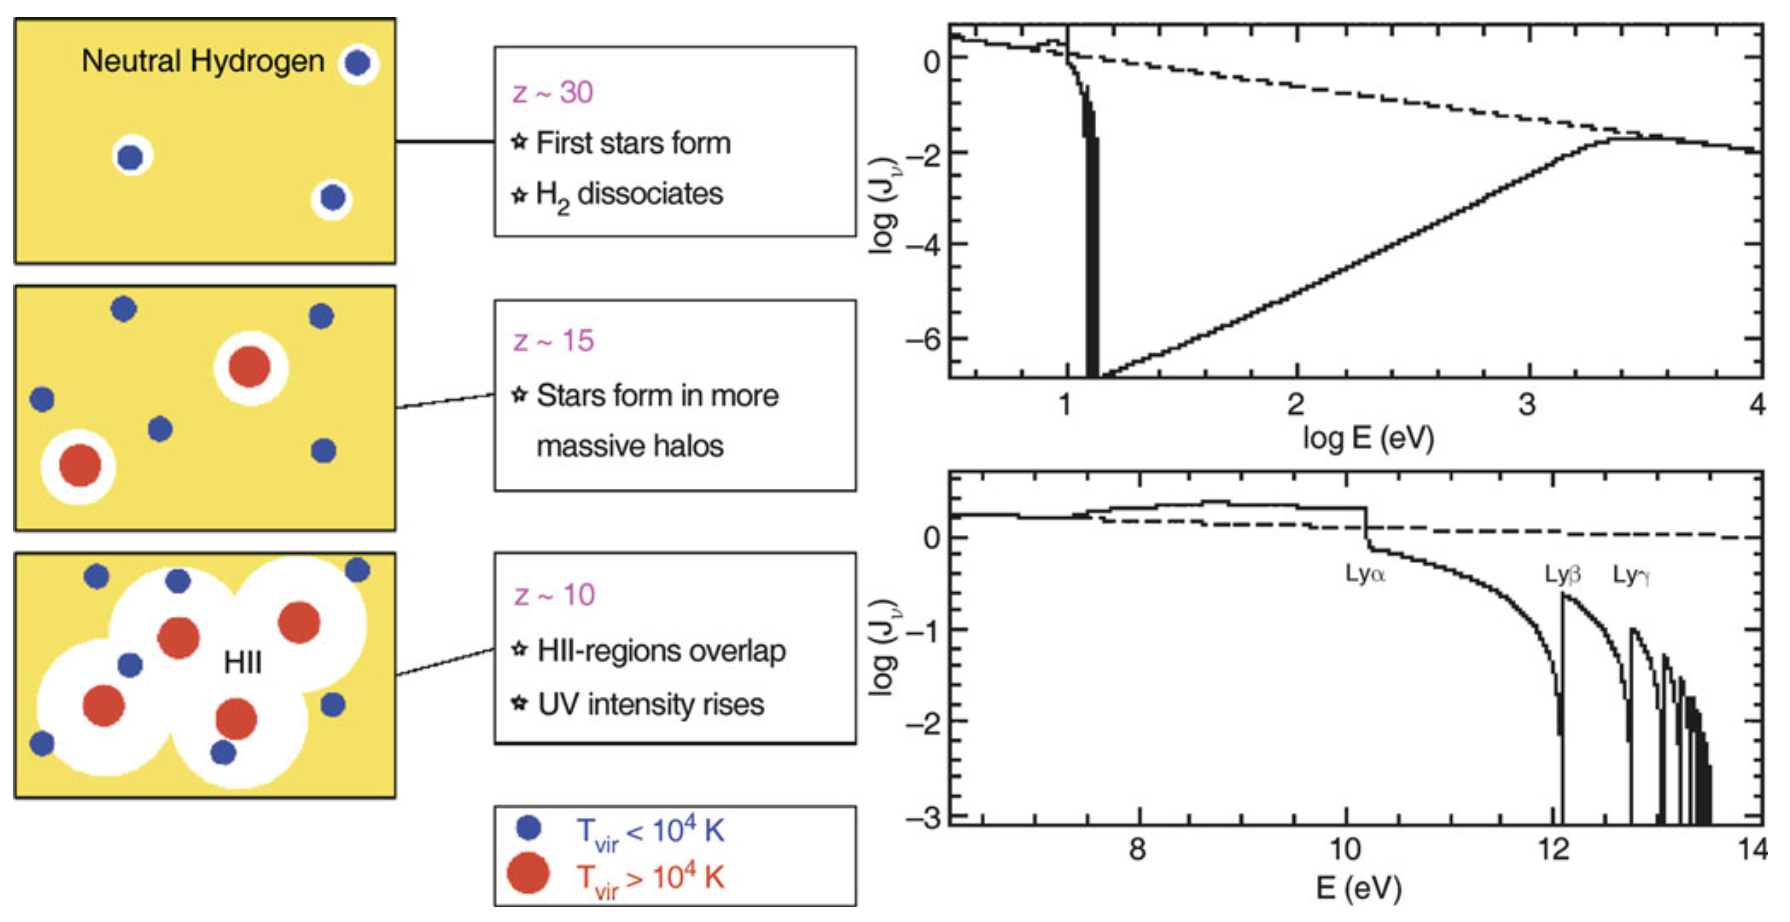
\includegraphics[width=16cm]{figures/reionization.png}
    \centering
    \caption{\footnotesize{\textit{On the left}, a sketch of the geometry of reionization is shown: initially, relatively low-mass halos collapse, a first generation of stars ionizes and heats the gas in and around these halos. By heating, the temperature increases so strongly (to about $T\sim10^4\,{\rm K}$) that gas can escape from the potential wells; these halos may never again form stars efficiently. Only when more massive halos have collapsed will continuous star formation set in. Ionizing photons from this first generation of hot stars produce HII-regions around their halos, which is the onset of reionization. The regions in which hydrogen is ionized will grow until they start to overlap; at that time, the flux of ionizing photons will strongly increase. \textit{On the right}, the average spectrum of photons at the beginning of the reionization epoch is shown; here, it has been assumed that the flux from the radiation source follows a power law (dashed curve). Photons with an energy higher than that of the Ly$\alpha$ transition are strongly suppressed because they are efficiently absorbed. The spectrum near the Lyman limit shows features which are produced by the combination of breaks corresponding to the various Lyman lines, and the redshifting of the photons. Source: R. Barkana \& A. Loeb 2000, In the Beginning: The First Sources of Light and the Reionization of the Universe, astro-ph/0010468, Figs. 4, 11. Image taken from Ryden (2006).}}
    \label{fig:reionization}
\end{figure}

{\noindent}We therefore conclude that reionization is a two-stage process. In a first phase, population III stars form through cooling of gas by molecular hydrogen, which is then destroyed by these very stars. Only in a later epoch and in more massive halos cooling is provided by atomic hydrogen, leading to reionization.

{\noindent}The increase of temperature causes an increase of the Jeans mass, due to its dependence on the sound speed. Once the IGM is heated to $\sim10^4\,{\rm K}$ by intergalactic UV radiation, the gas pressure prevents gas inflow into low-mass halos, corresponding to circular velocities $\lesssim30\,{\rm km\,s^{-1}}$. For this reason, one expects that halos of lower mass have a lower baryon fraction than that of the cosmic mixture, $f_b=\Omega_b/\Omega_m$. The actual value of the baryon fraction depends on the details of the merger history of a halo. Quantitative studies yield an average baryon mass of

\begin{align*}
    \bar{M}_b = \frac{f_b M}{[1+(2^{\alpha/3}-1)(M_C/M)^\alpha]^{3/\alpha}},
\end{align*}

{\noindent}where $M_C\sim10^9\,{\rm M_\odot}$ is a characteristic mass, defined such that for a halo with mass $M_C$, $\bar{M}_b/M=f_b/2$. For halos of mass smaller than $M_C$, the baryon fraction is suppressed, decreasing as $(M/M_C)^3$ for small masses, whereas for halo masses $\gg M_C$, the baryon fraction corresponds to the cosmic average. The index $\alpha\sim2$ determines the sharpness of the transition between these two cases. The characteristic mass $M_C$ depends on redshift, being much smaller at high $z$ due to the stronger ionizing background.

{\noindent}The ionizing flux has two additional effects on the gas that resides in halos: it provides a source of heating due to photoionization and it leads to a higher degree of ionization in the gas, reducing the number density of atoms which can be excited by collisions and cool through de-excitation. Both effects act in the same direction, by impeding an efficient cooling of the gas and hence the formation of stars. For halos of larger mass, intergalactic radiation is of fairly little importance because the corresponding heating rate is substantially smaller than that occurring by the dissipation of the gas which is needed to concentrate the baryons towards the halo center. For low-mass halos, however, this effect is important. Together, these two effects reduce the cooling rate of the gas, which is a dominant effect for low-mass halos. Thus, the gas in low-mass halos cannot cool efficiently, suppressing star formation -- unless star formation occurred before the reionization was completed. We hence found one of the elements for the second part of the answer to the question about the different mass-to-light ratios in halos: star formation in low mass halos is strongly suppressed due to the ionizing background radiation. This also provides an explanation of the `missing satellite problem'.

{\noindent}To singly ionize helium, photons of energy $\geq24.6\,{\rm eV}$ are required, and the ionization energy of He II is four times that of hydrogen. In addition, the recombination rate of fully ionized helium is about five times higher than that of hydrogen. Therefore, the reionization of helium is expected to be completed at a later epoch when the density of photons with $\lambda<304$\,\AA was high enough. Since even massive stars do not generate photons exceeding this energy in large quantities, the photons leading to helium reionization presumably are emitted by quasars; therefore, the ionization of helium has to wait for the `quasar epoch' of the Universe, at $z\lesssim4$. From the statistical analysis of the Ly$\alpha$ forest and from the analysis of helium absorption lines and the helium Gunn-Peterson effect in high-redshift QSOs, a reionization redshift of $z\sim3$ for helium is obtained.

{\noindent}One of the challenges of current observational cosmology is to link the history of reionization, as outlined above, to the observation of the highest redshift sources (i.e., to see whether we can observe the sources which are responsible for cosmic reionization). Are the galaxy populations that we can find at very high redshifts sufficient to understand the reionization process? Here we shall mention some of the major obstacles for a direct observation probe of these ionizing sources.

\begin{figure}[t]
    \floatbox[{\capbeside\thisfloatsetup{capbesideposition={right,top},capbesidewidth=4cm}}]{figure}[\FBwidth]
    {\caption{\footnotesize{The spectra of three high-redshift QSOs (SDSSJ1148+5251 at $z=6.42$, SDSS J1030+0524 at $z=6.31$, and the $z=7.085$ QSO ULAS J1120+0641) at the Lyman$\alpha$ emission line. For this figure, the wavelength difference to the Lyman$\alpha$ transition is expressed in proper distance away from the QSOs. The spectra are normalized, dividing them by the extrapolation of the continuum on the red side of the emission line, yielding the transmission. Source: D.J. Mortlock et al. 2011, A luminous quasar at a redshift of $z=7.085$, Nature 474, 616, Fig. 3. Figure taken from Ryden (2006).}}
    \label{fig:qsoreionization}}
    {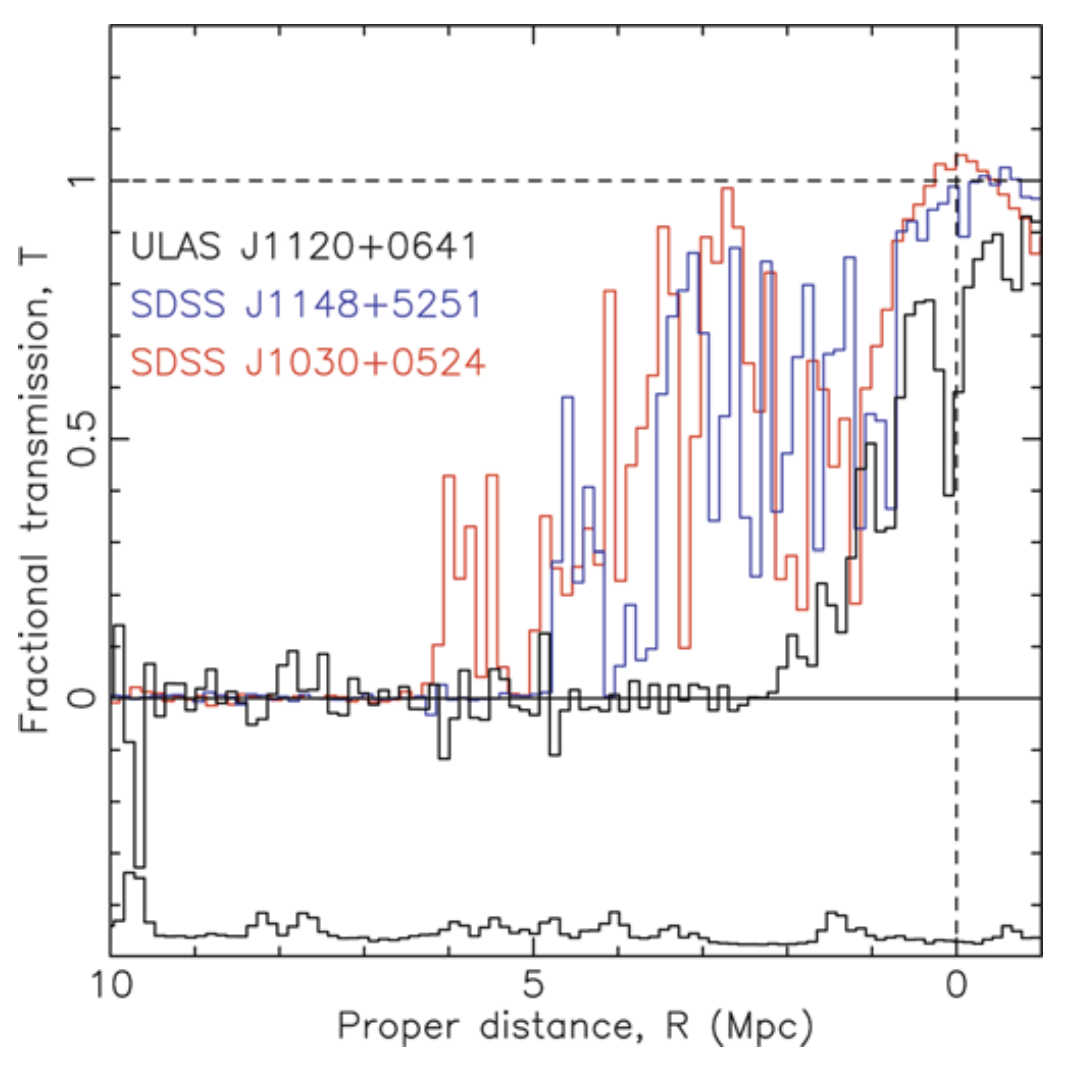
\includegraphics[width=9cm]{figures/QSOreionization.png}}
\end{figure}

{\noindent}If reionization was caused by the energetic photons emitted during star formation, the remnants of this first generation of stars must be present in the post-reionization Universe, and thus be observable. Galaxies at redshift $z>6$ are observed, either as Lyman-break galaxies (LBGs), Lyman-alpha emitters (LAEs) or as sub-millimeter galaxies (SMGs). Their stellar masses can be estimated from their observed light. However, most of the LBGs are observed only in the near-IR, which means that we see their restframe UV-emission. Converting the UV-light into a stellar mass is highly uncertain, since it depends strongly on the instantaneous star-formation rate. For LAEs, it is even more challenging to determine a stellar mass, since they are typically fainter in their broad-band (i.e., continuum) emission, which renders the determination of the stellar mass even more challenging.

{\noindent}Nevertheless, galaxies at very high redshift were found which appear to have high stellar masses, including a LAE at $z=6.6$ with an estimated stellar mass $M_*\gtrsim10^{11}\,{\rm M_\odot}$. The high-redshift QSOs require a SMBH with $M\gtrsim10^9\,{\rm M_\odot}$ to power their energy output, and these must be hosted in galaxies with very large stellar masses. Therefore, massive galaxies have formed very early on, delivering ionizing photons.

{\noindent}However, these highest mass objects are very rare and, by themselves, by far not able to explain reionization. This fact can be clearly seen by considering the spectral shape of the Ly$\alpha$ emission line of high-redshift QSOs. Figure \ref{fig:qsoreionization} shows the spectrum of three very high redshift QSOs near to the Lyman$\alpha$̨ emission line. Whereas all three QSO show essentially no flux blueward of Lyman$\alpha$, once the wavelength difference exceeds $\sim20$ {\AA} in the restframe, there is some transmitted flux very close to the Ly$\alpha$ transition. This near-zone transmission is understood as a region around the QSO where the intergalactic gas is fully ionized by the QSO, so it becomes transparent. The figure shows a clear trend that the size of this near zone decreases for higher redshifts, as would be expected due to the higher gas density and probably larger mean neutral fraction in the Universe. Thus, these very luminous objects are able to reionize the IGM in their immediate surroundings, but their effect is constrained to a rather limited volume. Most of the ionizing photons must come from the far more numerous lower-mass galaxies (i.e., far less luminous sources).

{\noindent}Gunn \& Peterson (1965) first proposed using Ly$\alpha$ resonance absorption in the spectrum of distant quasars as a direct probe to the neutral hydrogen density in the IGM at high redshift. For objects beyond reionization, neutral hydrogen in the IGM creates complete GP absorption troughs in the quasar spectrum blueward of Ly$\alpha$ emission. Observations of the GP effect directly constrain the evolution of neutral hydrogen fraction and the ionization state of the IGM.

{\noindent}The Gunn-Peterson optical depth to Ly$\alpha$ photons is

\begin{align*}
    \tau_\mathrm{GP} = \frac{\pi e^2}{m_ec^2}f_\alpha\lambda_\alpha H^{-1}(z)n_\mathrm{HI} ~ [{\rm dimensionless}],
\end{align*}

{\noindent}where $f_\alpha$ is the oscillator strength of the Ly$\alpha$ transition, $\lambda_\alpha=1216$\,\AA, $H(z)$ is the
Hubble constant at redshift $z$, and $n_\mathrm{HI}$ is the density of neutral hydrogen in the IGM.

{\noindent}At high redshifts,

\begin{align*}
    \tau_\mathrm{GP}(z) = 4.9\times10^5 \left(\frac{\Omega_mh^2}{0.13}\right)^{-1/2} \left(\frac{\Omega_bh^2}{0.02}\right) \left(\frac{1+z}{7}\right)^{3/2} \left(\frac{n_\mathrm{HI}}{n_\mathrm{H}}\right) ~ [{\rm dimensionless}]
\end{align*}

{\noindent}for a uniform IGM. Even a tiny neutral fraction, $X_\mathrm{HI}\sim10^{-4}$, gives rise to complete GP absorption. This test is only sensitive at the end of the reionization when the IGM is already mostly ionized, and the absorption saturates for the higher neutral fraction in the earlier stage.

{\noindent}At $z<5$, the IGM absorption is resolved into individual Ly$\alpha$ forest lines; their number density increases strongly with redshift: $N_\alpha(z)\propto(1+z)$. Earlier attempts to study GP absorption concentrated on measuring the amount of flux between individual Ly$\alpha$ forest lines using high-resolution spectroscopy to place limits on the diffuse neutral IGM. However, at $z>5$, even with a moderately high resolution spectrum, Ly$\alpha$ forest lines overlap severely, making it impossible to find a truly ``line-free'' region.

{\noindent}A more accurate picture of the IGM evolution interprets the Ly$\alpha$ forest as a fluctuating GP effect: absorption arises from low-density gas in the IGM that is in approximate thermal equilibrium between photoionization heating by the UV background and adiabatic cooling due to the Hubble expansion, rather than as discrete Lyα$\alpha$ forest clouds. The neutral hydrogen fraction and therefore the GP optical depth
depend on the local density of the IGM. By studying the evolution of the average transmitted flux or effective optical depth, one can trace the evolution of the UV ionizing background and neutral fraction of the IGM. At high-redshift, the IGM is highly clumpy, which must be taken into account in order to estimate the IGM ionization from observations.

\begin{figure}[t]
    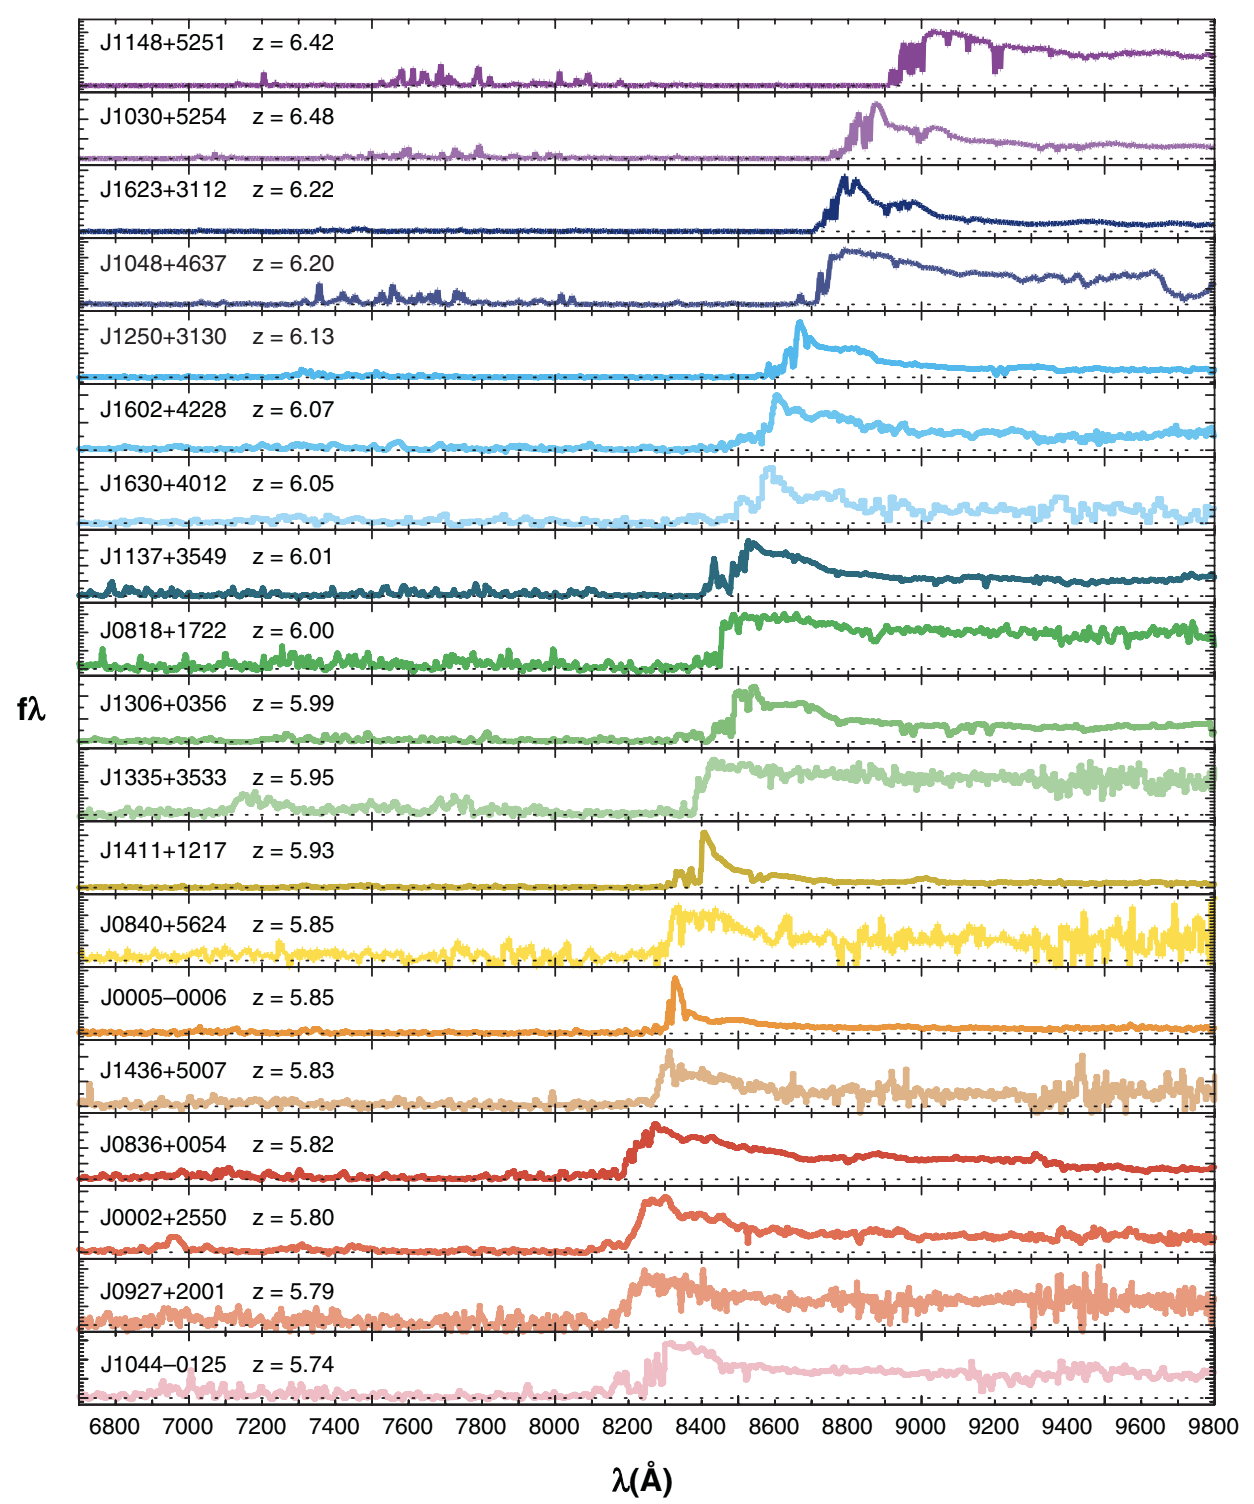
\includegraphics[width=14cm]{figures/SDSSQSO.png}
    \centering
    \caption{\footnotesize{Moderate resolution spectra of nineteen SDSS quasars at $5.74<z<6.42$. Adapted from Fan et al. (2006b). Image taken from Ryden (2006).}}
    \label{fig:sdssqso}
\end{figure}

{\noindent}The SDSS provides large samples of luminous quasars over $0<z<6.5$. Fan et al. (2000, 2001a,b, 2003, 2004, 2006a) carried out a survey of i-dropout quasars ($z>5.7$) using the SDSS imaging data, resulting in the discovery of 19 luminous quasars in this redshift regime (Figure \ref{fig:sdssqso}). Other multicolour survey projects are also searching for quasars at similar redshifts. They provide by far the best probes of IGM evolution toward the end of the EoR.

\begin{figure}[t]
    \floatbox[{\capbeside\thisfloatsetup{capbesideposition={right,top},capbesidewidth=4cm}}]{figure}[\FBwidth]
    {\caption{\footnotesize{Redshift evolution of the mean neutral fraction of hydrogen in the IGM, as obtained from the absorption of ionizing radiation from high-redshift QSOs (Gunn-Peterson effect). Individual measurements are shown as small dots, whereas the large circles with error bars represent averages over redshift bins. The two curves show results from numerical simulations. Source: X. Fan et al. 2006, Constraining the Evolution of the Ionizing Background and the Epoch of Reionization with $z\sim6$ Quasars. II. A Sample of 19 Quasars, AJ 132, 117, p. 126, Fig. 7. Figure taken from Ryden (2006).}}
    \label{fig:hivsz}}
    {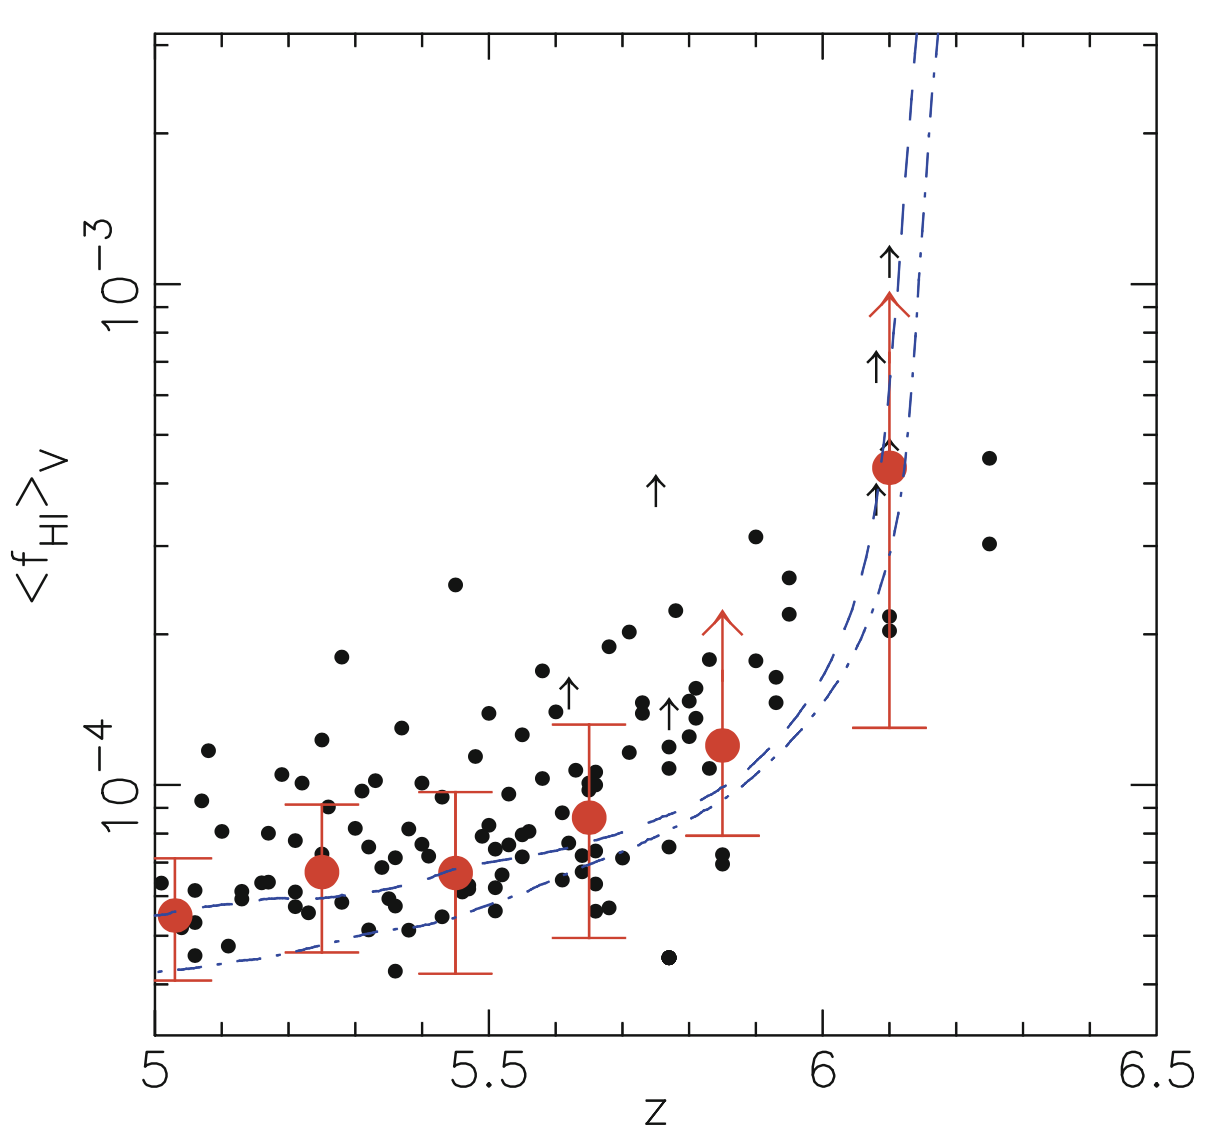
\includegraphics[width=10cm]{figures/HIvsz.png}}
\end{figure}

{\noindent}The observed spectrum of high-redshift QSOs bluewards of the Ly$\alpha$ emission line shows that an increasing fraction of the radiation is absorbed by neutral hydrogen on the line-of-sight. We have seen that the density of the Ly$\alpha$ forest increases with redshift (see Figures \ref{fig:qsoabsorption} and \ref{fig:sdssqso}) in such a way that only a tiny fraction of ionizing photons manage to escape absorption. This observation may be seen as an indication that we approach the EoR as the QSO redshift increases beyond $z\sim6$. However, as shown in Figure \ref{fig:hivsz}, the mean neutral fraction of intergalactic hydrogen needed to cause this strong absorption of ionizing photons is still very small -- a neutral fraction of much less than 1\% is sufficient to entirely block the light of QSOs blueward of the Ly$\alpha$ emission. Hence, the strong absorption implied by QSO spectra cannot be taken as evidence for $z\sim6$ signalling the end of the EoR. Nevertheless, the trend of the data shown in Figure \ref{fig:hivsz} may suggest that beyond $z\sim6$, we may approach a phase where the neutral hydrogen fraction indeed starts to increase significantly.

{\noindent}Observing reionization directly may in principle be possible if a very high-redshift QSO could be identified whose absorption spectrum could reveal a tomographic view through the ionized `bubbles' of the IGM, as sketched in Figure \ref{fig:lyaforest}. But we point out again that the very dense Ly$\alpha$ forest seen towards QSOs at high redshift, is no unambiguous sign for approaching the redshift of reionization, because a very small fraction of neutral atoms (about 1\%) is already sufficient to produce a large optical depth for Ly$\alpha$ photons.

\begin{figure}[h!]
    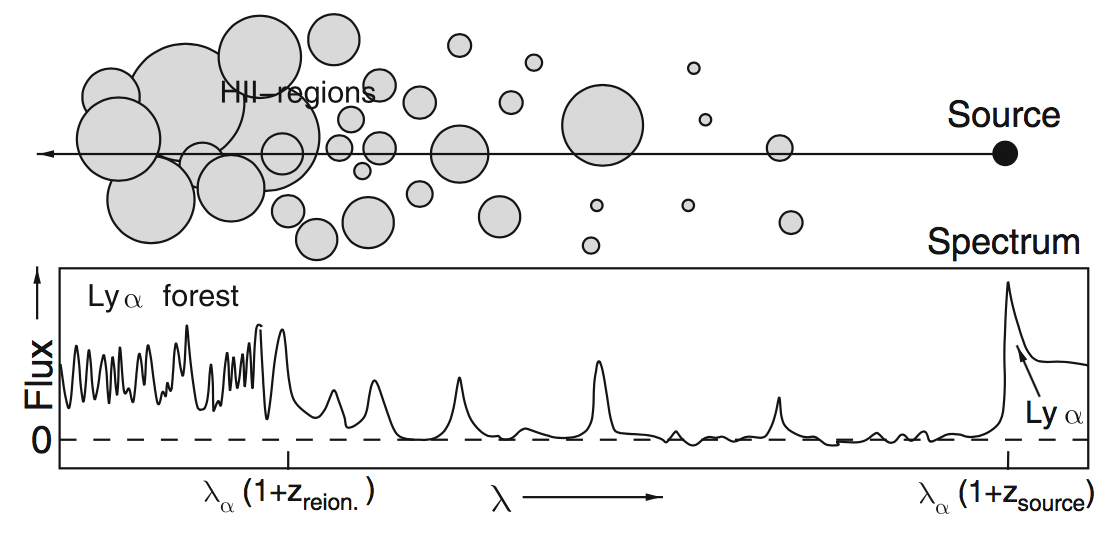
\includegraphics[width=14cm]{figures/LyaForest.png}
    \centering
    \caption{\footnotesize{Sketch of a potential observation of reionization: light from a very distant QSO propagates through a partially ionized Universe; at locations where it passes through HII-regions, radiation will get through -- flux will be visible at the corresponding wavelengths. When the HII-regions start to overlap, the normal Ly$\alpha$ forest will be produced. Adapted from: R. Barkana \& A. Loeb 2000, In the Beginning: The First Sources of Light and the Reionization of the Universe, astro-ph/0010468. Figure taken from Ryden (2006).}}
    \label{fig:lyaforest}
\end{figure}

\subsubsection{Follow-up Questions}

\begin{itemize}
    \item Besides the first stars and galaxies, what else could have ionized the Universe?
    \item How does the recent paper by Bowman et al. relate to this?
\end{itemize}


% --------------------------------------------------------------
%
%                           16. 
%
% --------------------------------------------------------------

\newpage
\subsection{Question 16}

The $21\,{\rm cm}$ line of hydrogen is expected to show up in absorption against the cosmic microwave background at some redshifts, and in emission at other redshifts. What physical processes lead to this behaviour?

\subsubsection{Short answer}

The key to the detectability of the $21\,{\rm cm}$ signal hinges on the spin temperature $T_s$. Only if this temperature deviates from the background temperature, will a signal be observable.

\begin{itemize}
    \item $\mathbf{200\lesssim z\lesssim 1100:}$ The residual free electron fraction left after recombination allows Compton scattering to maintain thermal coupling of the gas to the CMB, setting $T_k=T_\gamma$. The high gas density leads to effective collisional coupling so that $T_s=T_\gamma$ and we expect $\bar{T}_b=0$ and no detectable $21\,{\rm cm}$ signal.
    \item $\mathbf{40\lesssim z\lesssim 200:}$In this regime, the gas cools adiabatically so that $T_k\propto(1+z)^2$ leading to $T_k<T_\gamma$ and collisional coupling sets $T_s<T_\gamma$, leading to $\bar{T}_b<0$ and an early absorption signal. At this time, $T_b$ fluctuations are sourced by density fluctuations, potentially allowing the initial conditions to be probed.
    \item $\mathbf{z_*\lesssim z\lesssim 40:}$ As the expansion continues, decreasing the gas density, collisional coupling becomes ineffective and radiative coupling to the CMB sets $T_s=T_\gamma$, and there is no detectable $21\,{\rm cm}$ signal.
    \item $\mathbf{z_\alpha\lesssim z\lesssim z_*:}$ Once the first sources switch on at $z_*$, they emit both Ly$\alpha$ photons and X-rays. In general, the emissivity required for Ly$\alpha$ coupling is significantly less than that for heating $T_k$ above $T_\gamma$. We therefore expect a regime where the spin temperature is coupled to cold gas so that $T_s\sim T_k<T_\gamma$ and there is an absorption signal. Fluctuations are dominated by density fluctuations and variation in the Ly$\alpha$ flux. As further star formation occurs the Ly$\alpha$ coupling will eventually saturate ($x_\alpha\gg1$), so that by a redshift $z_\alpha$ the gas will everywhere be strongly coupled.
    \item $\mathbf{z_h\lesssim z\lesssim z_\alpha:}$ After Ly$\alpha$ coupling saturates, fluctuations in the Ly$\alpha$ flux no longer affect the $21\,{\rm cm}$ signal. By this point, heating becomes significant and gas temperature fluctuations source $T_b$ fluctuations. While $T_k$ remains below $T_\gamma$ we see a $21\,{\rm cm}$ signal in absorption, but as $T_k$ approaches $T_\gamma$ hotter regions may begin to be seen in emission. Eventually by a redshift $z_h$ the gas will be heated everywhere so that $\bar{T}_k=T_\gamma$.
    \item $\mathbf{z_T\lesssim z\lesssim z_h:}$ After the heating transition, $T_k>T_\gamma$ and we expect to see a $21\,{\rm cm}$ signal in emission. The $21\,{\rm cm}$ brightness temperature is not yet saturated, which occurs at $z_T$, when $T_s\sim T_k\gg T_\gamma$. By this time, the ionization fraction has likely risen above the percent level. Brightness temperature fluctuations are sourced by a mixture of fluctuations in ionization, density and gas temperature.
    \item $\mathbf{z_r\lesssim z\lesssim z_T:}$ Continued heating drives $T_k\gg T_\gamma$ at $z_T$ and temperature fluctuations become unimportant. $T_s\sim T_k\gg T_\gamma$ and the dependence on $T_s$ may be neglected which greatly simplifies analysis of the $21\,{\rm cm}$ power spectrum. By this point, the filling fraction of HII regions probably becomes significant and ionization fluctuations begin to dominate the $21\,{\rm cm}$ signal.
    \item $\mathbf{z\lesssim z_r:}$ After reionization, any remaining $21\,{\rm cm}$ signal originates primarily from collapsed islands of neutral hydrogen (damped Ly$\alpha$ systems).
\end{itemize}

{\noindent}These events are summarized in Figure \ref{fig:21cmannotated}.

\begin{figure}[t]
    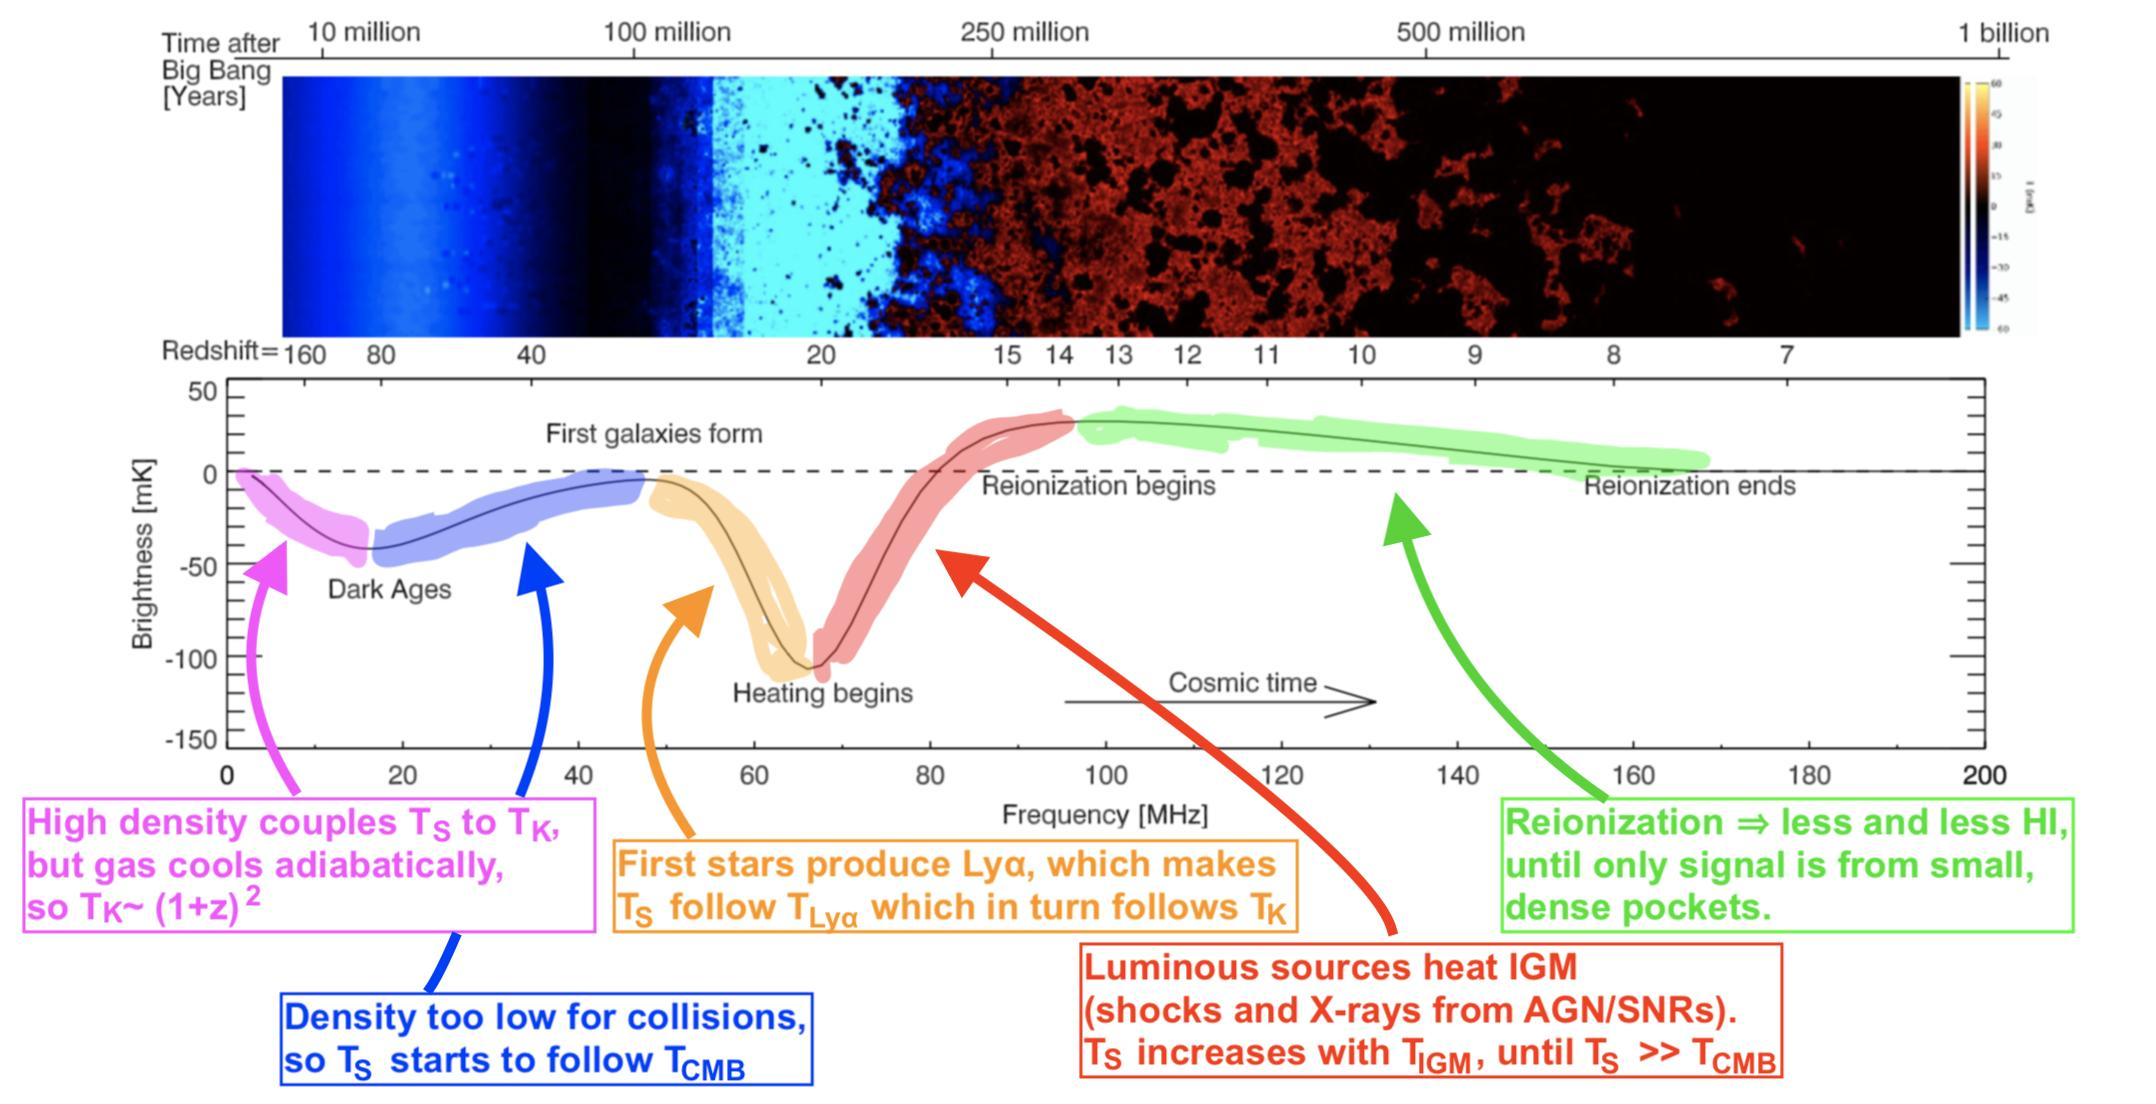
\includegraphics[width=16cm]{figures/21cm_annotated.jpg}
    \centering
    \caption{\footnotesize{The 21-centimeter cosmic hydrogen signal.}}
    \label{fig:21cmannotated}
\end{figure}

\subsubsection{Additional context}

{\noindent}As the most common atomic species present in the Universe, hydrogen is a useful tracer of local properties of the gas. The simplicity of its structure (a proton and electron) belies the richness of the associated physics. The $21\,{\rm cm}$ line of hydrogen arises from the hyperfine splitting of the $1S$ ground state due to the interaction of the magnetic moments of the proton and the electron. This splitting leads to two distinct energy levels separated by $\Delta E_{21\,\mathrm{cm}}=5.9\times10^{-6}\,{\rm eV}$, corresponding to a wavelength of $21\,{\rm cm}$ and a frequency of $1420\,{\rm MHz}$. This frequency is one of the most precisely known quantities in astrophysics having been measured to great accuracy from studies of hydrogen masers.

{\noindent}Radio telescopes look for emission by warm hydrogen gas within galaxies. Since the line is narrow with a well measured rest frame frequency it can be used in the local Universe as a probe of the velocity distribution of gas within our galaxy and other nearby galaxies. $21\,{\rm cm}$ rotation curves are often used to trace galactic dynamics. Traditional techniques for observing $21\,{\rm cm}$ emission have only detected the line in relatively local galaxies, although it has been seen in absorption against radio loud background sources from individual systems at redshifts $z\lesssim3$. A new generation of radio telescopes offers the exciting prospect of using the $21\,{\rm cm}$ line as a probe of cosmology.

{\noindent}In cosmological contexts the $21\,{\rm cm}$ line has been used as a probe of gas along the line of sight to some background radio source. The detailed signal depends upon the radiative transfer through gas along the line of sight. We recall the basic equation of radiative transfer (RT) for the specific intensity $I_\nu$ (per unit frequency $\nu$) in the absence of scattering along a path described by coordinate $s$

\begin{align*}
    \frac{\mathrm{d}I_\nu}{\mathrm{d}s} = j_\nu - \alpha_\nu I_\nu ~ [{\rm erg\,s^{-1}\,cm^{-2}\,Hz^{-1}\,sr^{-1}\,pc^{-1}}],
\end{align*}

{\noindent}where absorption and emission by gas along the path are described by the coefficients $\alpha_\nu$ and $j_\nu$, respectively.

{\noindent}To simplify the discussion, we will work in the Rayleigh-Jeans (RJ) limit, appropriate here since the relevant photon frequencies $\nu$ are much smaller than the peak frequency of the CMB blackbody. This allows us to relate the intensity $I_\nu$ to a brightness temperature $T_b$ by the relation $I_\nu=2k_BT\nu^2/c^2$, where $c$ is the speed of light and $k_B$ is Boltzmann's constant. We will also make use of the standard definition of the optical depth $\tau=\int\alpha_\nu\mathrm{d}s$. With this we may rewrite the equation of RT to give the radiative transfer for light from a background radio source of brightness temperature $T_r$ (primarily the CMB) along the line of sight through a cloud of optical depth $\tau_\nu$ and uniform excitation temperature $T_\mathrm{ex}$ so that the observed brightness temperature $T_b^\mathrm{obs}$ at a frequency $\nu$ is given by

\begin{align*}
    T_b^\mathrm{obs} = T_\mathrm{ex}(1-e^{-\tau_\nu})+T_r(\nu)e^{-\tau_\nu} ~ [{\rm K}].
\end{align*}

{\noindent}Figure \ref{fig:21cm} provides a summary of the $21\,{\rm cm}$ signal showing the key features of the signal with the relevant cosmic time, frequency, and redshift scales indicated. The earliest period of the signal arises in the period after thermal decoupling of the ordinary matter (baryons) from the CMB, so that the gas is able to cool adiabatically with the expansion of the Universe. In these cosmic ``Dark Ages'', before the first stars have formed, the first structures begin to grow from the seed inhomogeneties thought to be produced by quantum fluctuations during inflation. The cold gas can be seen in a $21\,{\rm cm}$ absorption signal, which has both a mean value (shown in the bottom panel) and fluctuations arising from variation in density (shown in the top panel). Once the first stars and galaxies form, their light radically alters the properties of the gas. Scattering of Ly$\alpha$ photons leads to a strong coupling between the excitation of the $21\,{\rm cm}$ line spin states and the gas temperature. Initially, this leads to a strong absorption signal that is spatially varying due to the strong clustering of the rare first generation of galaxies. Next, the X-ray emission from these galaxies heats the gas leading to a $21\,{\rm cm}$ emission signal. Finally, ultraviolet photons ionize the gas producing dark holes in the $21\,{\rm cm}$ signal within regions of ionized bubbles surrounding groups of galaxies. Eventually all of the hydrogen gas, except for that in a few dense pockets, is ionized.

\begin{figure}[t]
    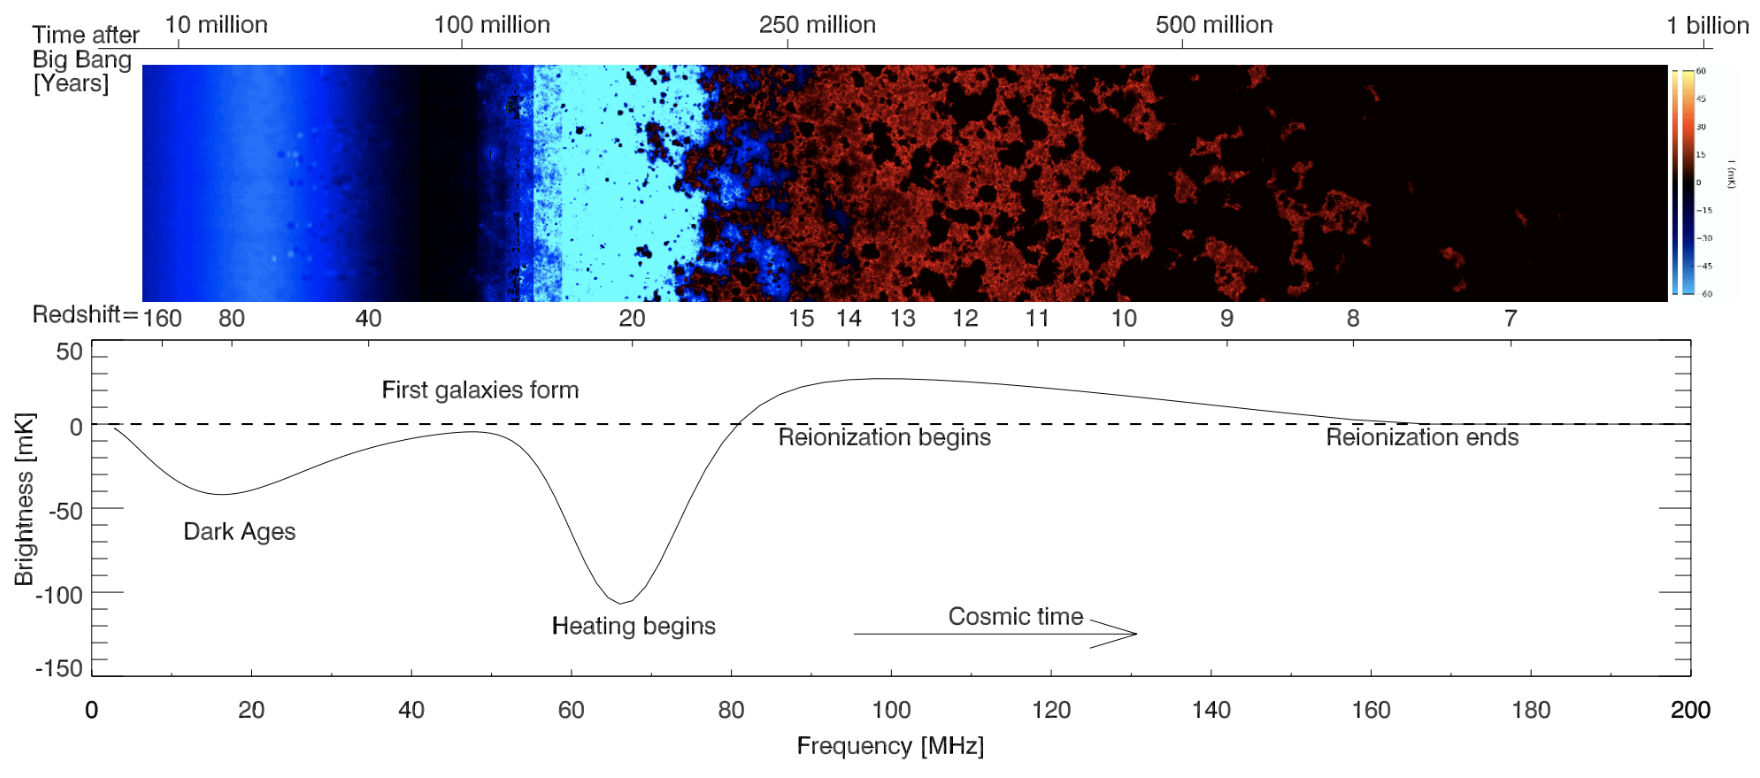
\includegraphics[width=16cm]{figures/21cm.png}
    \centering
    \caption{\footnotesize{The 21-centimeter cosmic hydrogen signal. (a) Time evolution of fluctuations in the $21\,{\rm cm}$ brightness from just before the first stars formed through to the end of the EoR. This evolution is pieced together from redshift slices through a simulated cosmic volume. Colouration indicates the strength of the $21\,{\rm cm}$ brightness as it evolves through two absorption phases (purple and blue), separated by a period (black) where the excitation temperature of the $21\,{\rm cm}$ hydrogen transition decouples from the temperature of the hydrogen gas, before it transitions to emission (red) and finally disappears (black) owing to the ionization of the hydrogen gas. (b) Expected evolution of the sky-averaged $21\,{\rm cm}$ brightness from the ``dark ages'' at redshift $200$ to the end of reionization, sometime before redshift $6$ (solid curve indicates the signal; dashed curve indicates $T_b=0$). The frequency structure within this redshift range is driven by several physical processes, including the formation of the first galaxies and the heating and ionization of the hydrogen gas. There is considerable uncertainty in the exact form of this signal, arising from the unknown properties of the first galaxies. Figure taken from Ryden (2006).}}
    \label{fig:21cm}
\end{figure}

{\noindent}The excitation temperature of the $21\,{\rm cm}$ line is known as the spin temperature $T_s$. It is defined through the ratio between the number densities $n_i$ of hydrogen atoms in the two hyperfine levels (which we label with a subscript $0$ and $1$ for the $1S$ singlet and $1S$ triplet levels, respectively)

\begin{align*}
    \frac{n_1}{n_2} = \frac{g_1}{g_2}\exp\left(-\frac{T_*}{T_s}\right) ~ [{\rm dimensionless}],
\end{align*}

{\noindent}where $(g_1/g_0)=3$ is the ratio of the statistical degeneracy factors of the two levels, and $T_*\equiv hc/k_B\lambda_{21\,\mathrm{cm}}=0.068\,{\rm K}$.

{\noindent}With this definition, the optical depth of a cloud of hydrogen is then

\begin{align*}
    \tau_\nu = \int \left[1-\exp\left(-\frac{E_{10}}{k_BT_s}\right)\right]\sigma_0\phi(\nu)n_0\mathrm{d}s ~ [{\rm dimensionless}],
\end{align*}

{\noindent}where $n_0=n_\mathrm{H}/4$ with $n_\mathrm{H}$ being the hydrogen density, and we have denoted the $21\,{\rm cm}$ cross-section as $\sigma(\nu)=\sigma_0\phi(\nu)$, with $\sigma_0\equiv3c^22A_{10}/8\pi\nu^2$, where $A_{10}=2.85\times10^{-15}\,s^{-1}$ is the spontaneous decay rate of the spin-flip transition, and the line profile is normalized so that $\int\phi(\nu)\mathrm{d}\nu=1$. To evaluate this expression we need to find the column length as a function of frequency $s(\nu)$ to determine the range of frequencies $\mathrm{d}\nu$ over the path $\mathrm{d}s$ that correspond to a fixed observed frequency $\nu_\mathrm{obs}$. This can be done in one of two ways: by relating the path length to the cosmological expansion $\mathrm{d}s=−c\mathrm{d}z/(1+z)H(z)$ and the redshifting of light to relate the observed and emitted frequencies $\nu_\mathrm{obs}=\nu_\mathrm{em}/(1+z)$ or assuming a linear velocity profile locally $v=(\mathrm{d}\nu/\mathrm{d}s)s$ (the well known Sobolev approximation) and using the Doppler law $\nu_\mathrm{obs}=\nu_\mathrm{em}(1-v/c)$ self-consistently to $\mathcal{O}(v/c)$. Since the latter case describes the well known Hubble law in the absence of peculiar velocities these two approaches give identical results for the optical depth. The latter picture brings out the effect of peculiar velocities that modify the local velocity-frequency conversion.

{\noindent}The optical depth of this transition is small at all relevant redshifts, yielding a differential brightness temperature

\begin{align*}
    \delta T_b &= \frac{T_s-T_r}{1+z}(1-e^{-\tau_\nu}) \\
    &\approx \frac{T_s-T_r}{1+z}\tau \\
    &\approx 27x_\mathrm{HI}(1+f_b)\left(\frac{\Omega_bh^2}{0.023}\right)\left(\frac{0.15}{\Omega_mh^2}\frac{1+z}{10}\right)^{1/2}\left(\frac{T_s-T_r}{T_s}\right)\left(\frac{\partial_rv_r}{(1+z)H(z)}\right) ~ [{\rm mK}],
\end{align*}

{\noindent}Here $x_\mathrm{HI}$ is the neutral fraction of hydrogen, $f_b$ is the fractional overdensity in baryons,
and the final term arises from the velocity gradient along the line of sight $\partial_rv_r$.

{\noindent}The key to the detectability of the $21\,{\rm cm}$ signal hinges on the spin temperature. Only if this temperature deviates from the background temperature, will a signal be observable; the spin temperature and spatial variation in the spin temperature can be used to convey information about astrophysical sources.

{\noindent}Three processes determine the spin temperature: (i) absorption/emission of $21\,{\rm cm}$ photons from/to the radio background, primarily the CMB; (ii) collisions with other hydrogen atoms and with electrons; and (iii) resonant scattering of Ly$\alpha$ photons that cause a spin flip via an intermediate excited state. The rate of these processes is fast compared to the de-excitation time of the line, so that to a very good approximation the spin temperature is given by the equilibrium balance of these effects. In this limit,
the spin temperature is given by

\begin{align*}
    T_s^{-1} = \frac{T_\gamma^{-1} + x_\alpha T_\alpha^{-1} + x_cT_K^{-1}}{1+x_\alpha+x_c} ~ [{\rm K^{-1}}],
\end{align*}

{\noindent}where $T_\gamma$ is the temperature of the surrounding bath of radio photons, typically set by the CMB so that $T_\gamma=T_\mathrm{CMB}$; $T_\alpha$ is the colour temperature of the Ly$\alpha$ radiation field at the Ly$\alpha$ frequency and is closely coupled to the gas kinetic temperature $T_k$ by recoil during repeated scattering, and $x_c$, $x_\alpha$ are the coupling coefficients due to atomic collisions and scattering of Ly$\alpha$ photons, respectively. The spin temperature becomes strongly coupled to the gas temperature when $x_\mathrm{tot}\equiv x_c+x_\alpha\gtrsim1$ and relaxes to $T_\gamma$ when $x_\mathrm{tot}\ll1$.

{\noindent}Two types of background radio sources are important for the $21\,{\rm cm}$ line as a probe of astrophysics. Firstly, we may use the CMB as a radio background source. In this case, $T_r = T_\mathrm{CMB}$ and the $21\,{\rm cm}$ feature is seen as a spectral distortion to the CMB blackbody at appropriate radio frequencies (since fluctuations in the CMB temperature are small $\Delta T_\mathrm{CMB}\sim10^{-5}$ the CMB is effectively a source of uniform brightness). The distortion forms a diffuse background that can be studied across the whole sky in a similar way to CMB anisotropies. Observations at different frequencies probe different spherical shells of the observable Universe, so that a 3D map can be constructed.

{\noindent}The second situation uses a radio loud point source, for example a radio loud quasar, as the background. In this case, the source will always be much brighter than the weak emission from diffuse hydrogen gas, $T_r\gg T_s$, so that the gas is seen in absorption against the source. The appearance of lines from regions of neutral gas at different distances to the source leads to a ``forest'' of lines known as the ``$21\,{\rm cm}$ forest'' in analogy to the Ly$\alpha$ forest. The high brightness of the background source allows the $21\,{\rm cm}$ forest to be studied with high frequency resolution so probing small scale structures ($\sim\,{\rm kpc}$) in the IGM. For useful statistics, many lines of sight to different radio sources are required, making the discovery of high redshift radio sources a priority.

\begin{figure}[t]
    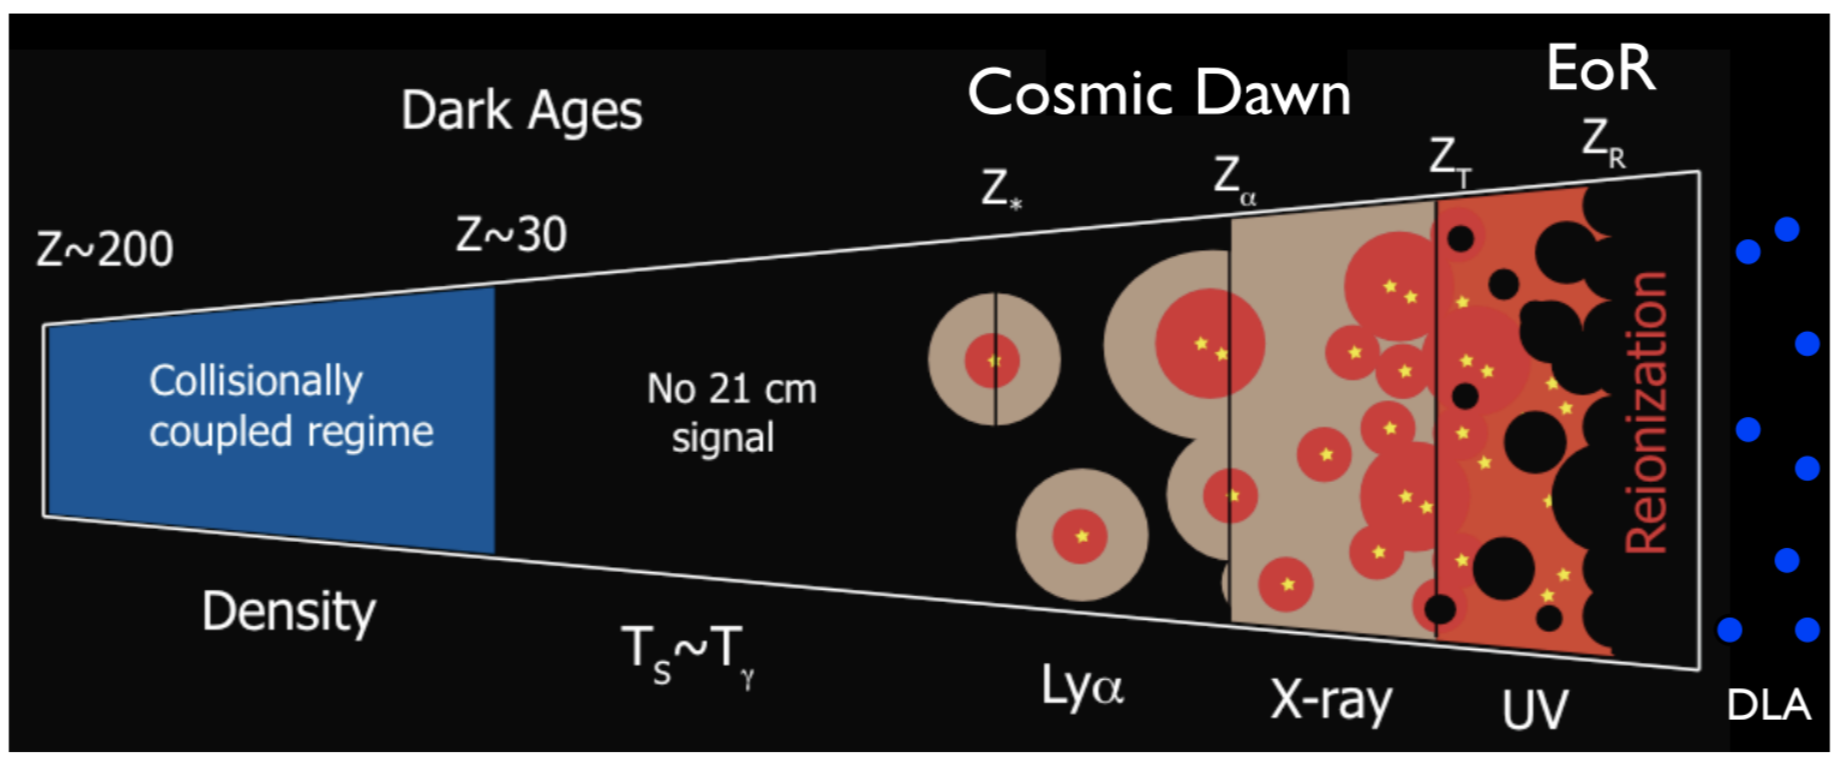
\includegraphics[width=16cm]{figures/21cm_schematic.png}
    \centering
    \caption{\footnotesize{Cartoon of the different phases of the $21\,{\rm cm}$ signal. The signal transitions from an early phase of collisional coupling to a later phase of Ly$\alpha$ coupling through a short period where there is little signal. Fluctuations after this phase are dominated successively by spatial variation in the Ly$\alpha$, X-ray, and ionizing UV radiation backgrounds. After reionization is complete there is a residual signal from neutral hydrogen in galaxies. Figure taken from Ryden (2006).}}
    \label{fig:21cmschematic}
\end{figure}

{\noindent}Collisions between different particles may induce spin-flips in a hydrogen atom and dominate the coupling in the early Universe where the gas density is high. Three main channels are available: collisions between two hydrogen atoms and collisions between a hydrogen atom and an electron or a proton. The collisional coupling for a species is

\begin{align*}
    x_c^i \equiv \frac{C_{10}}{A_{10}}\frac{T_*}{T_\gamma} = \frac{n_ik_{10}^i}{A_{10}}\frac{T_*}{T_\gamma},
\end{align*}

{\noindent}where $C_{10}$ is the collisional excitation rate, $k_{10}^i$ is the specific rate coefficient for spin de-excitation by collisions with species $i$ (in units of $cm^3s^{-1}$).

{\noindent}The total collisional coupling coefficient can be written as

\begin{align*}
    x_c &= x_c^\mathrm{HH} + x_c^\mathrm{eH} + x_c^\mathrm{pH} \\
        &= \frac{T_*}{A_{10}T_\gamma} \left[k_{1-0}^\mathrm{HH}(T_k)n_\mathrm{H}+k_{1-0}^{e\mathrm{H}}(T_k)n_e+k_{1-0}^{p\mathrm{H}}(T_k)n_p\right] ~ [{\rm dimensionless}],
\end{align*}

{\noindent}where $k_{1-0}^\mathrm{HH}$ is the scattering rate between hydrogen atoms, $k_{1-0}^{e\mathrm{H}}$ is the scattering rate between hydrogen atoms and electrons, and $k_{1-0}^{p\mathrm{H}}$ is the scattering rate between hydrogen atoms and protons.

{\noindent}We may express the $21\,{\rm cm}$ brightness temperature as a function of four variables $T_b=T_b(T_k,x_i,J_\alpha,n_\mathrm{H})$, where $x_i$ is the volume-averaged ionized fraction of hydrogen and $J_\alpha$ is the Ly$\alpha$ specific flux. In calculating the $21\,{\rm cm}$ signal, we require a model for the global evolution of and fluctuations in these quantities. Before looking at the evolution of the signal quantitatively, we will first outline the basic picture to delineate the most important phases.

{\noindent}An important feature of $T_b$ is that its dependence on each of these quantities saturates at some point, for example once the Ly$\alpha$ flux is high enough the spin and kinetic gas temperatures become tightly coupled and further variation in $J_\alpha$ becomes irrelevant to the details of the signal. This leads to conceptually separate regimes where variation in only one of the variables dominating fluctuations in the signal. These different regimes can be seen in Figure \ref{fig:21cm} and are shown in schematic form in Figure \ref{fig:21cmschematic}.

% --------------------------------------------------------------
%
%                           17. 
%
% --------------------------------------------------------------

\newpage
\subsection{Question 17}

What is the difference between scalar and tensor modes of perturbation in the early universe, and how can you detect their presence?

\subsubsection{Short answer}

Short answer.

\subsubsection{Additional context}

{\noindent}Scalars, vectors, and tensors generate distinct patterns in the polarization of the CMB. However, although they separate cleanly into $m=0,\pm1,\pm2$ polarization patterns for a single plane wave perturbation in the coordinate system referenced to $k\bm{k}$, in general there will exist a spectrum of fluctuations each with a different $\bm{k}$. Therefore the polarization pattern on the sky does not separate into $m=0,\pm1,\pm2$ modes. In fact, assuming statistical isotropy, one expects the ensemble averaged power for each multipole $\ell$ to be independent of $m$. Nonetheless, certain properties of the polarization patterns do survive superposition of the perturbations: in particular, its parity and its correlation with the temperature fluctuations.

\begin{figure}[h]
    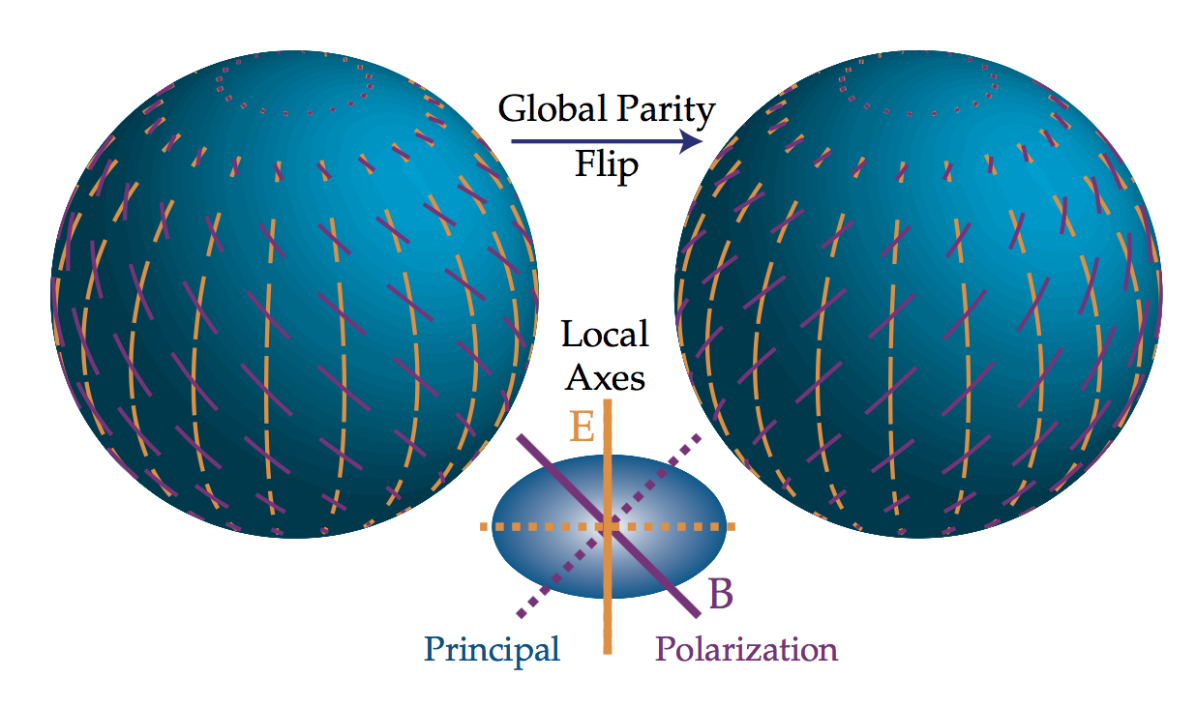
\includegraphics[width=16cm]{figures/EBmodes.png}
    \centering
    \caption{\footnotesize{The electric ($E$) and magnetic ($B$) modes are distinguished by their behavior under a parity transformation $\bm{\hat{n}}\rightarrow\bm{\hat{n}}$. $E$-modes have $(-1)^\ell$ and $B$-modes have $(-1)^{\ell+1}$ parity; here ($\ell=2,m=0$), even and odd respectively. The local distinction between the two is that the polarization axis is aligned with the principle axes of the polarization amplitude for $E$ and crossed with them for $B$. Dotted lines represent a sign reversal in the polarization. Image taken from Hu \& White (1997).}}
    \label{fig:ebmodes}
\end{figure}

{\noindent}\textbf{Scalar (compressible) perturbations}:

{\noindent}The most commonly considered and familiar types of perturbations are scalar modes. These modes represent perturbations in the (energy) density of the cosmological fluid(s) at last scattering and are the only fluctuations which can form structure though gravitational instability. Consider a single large-scale Fourier component of the fluctuation (i.e., for the photons, a single plane wave in the temperature perturbation). Over time, the temperature and gravitational potential gradients cause a bulk flow, or dipole anisotropy, of the photons. Both effects can be described by introducing an “effective” temperature

\begin{align*}
    \left(\frac{\Delta T}{T}\right)_\mathrm{eff} = \left(\frac{\Delta T}{T}\right) + \psi,
\end{align*}

{\noindent}where $\psi$ is the gravitational potential. Gradients in the effective temperature always create flows from hot to cold effective temperature. Formally, both pressure and gravity act as sources of the momentum density of the fluid in a combination that is exactly the effective temperature for a relativistic fluid.

{\noindent} To avoid confusion, let us explicitly consider the case of adiabatic fluctuations, where initial perturbations to the density imply potential fluctuations that dominate at large scales. Here gravity overwhelms pressure in overdense regions causing matter to flow towards density peaks initially. Nonetheless, overdense regions are effectively cold initially because photons must climb out of the potential wells they create and hence lose energy in the process. Though flows are established from cold to hot temperature regions on large scales, they still go from hot to cold effective temperature regions. This property is true more generally of our adiabatic assumption: we hereafter refer only to effective temperatures to keep the argument general.

\begin{figure}[t!]
    \centering
    \vspace{-1cm}
    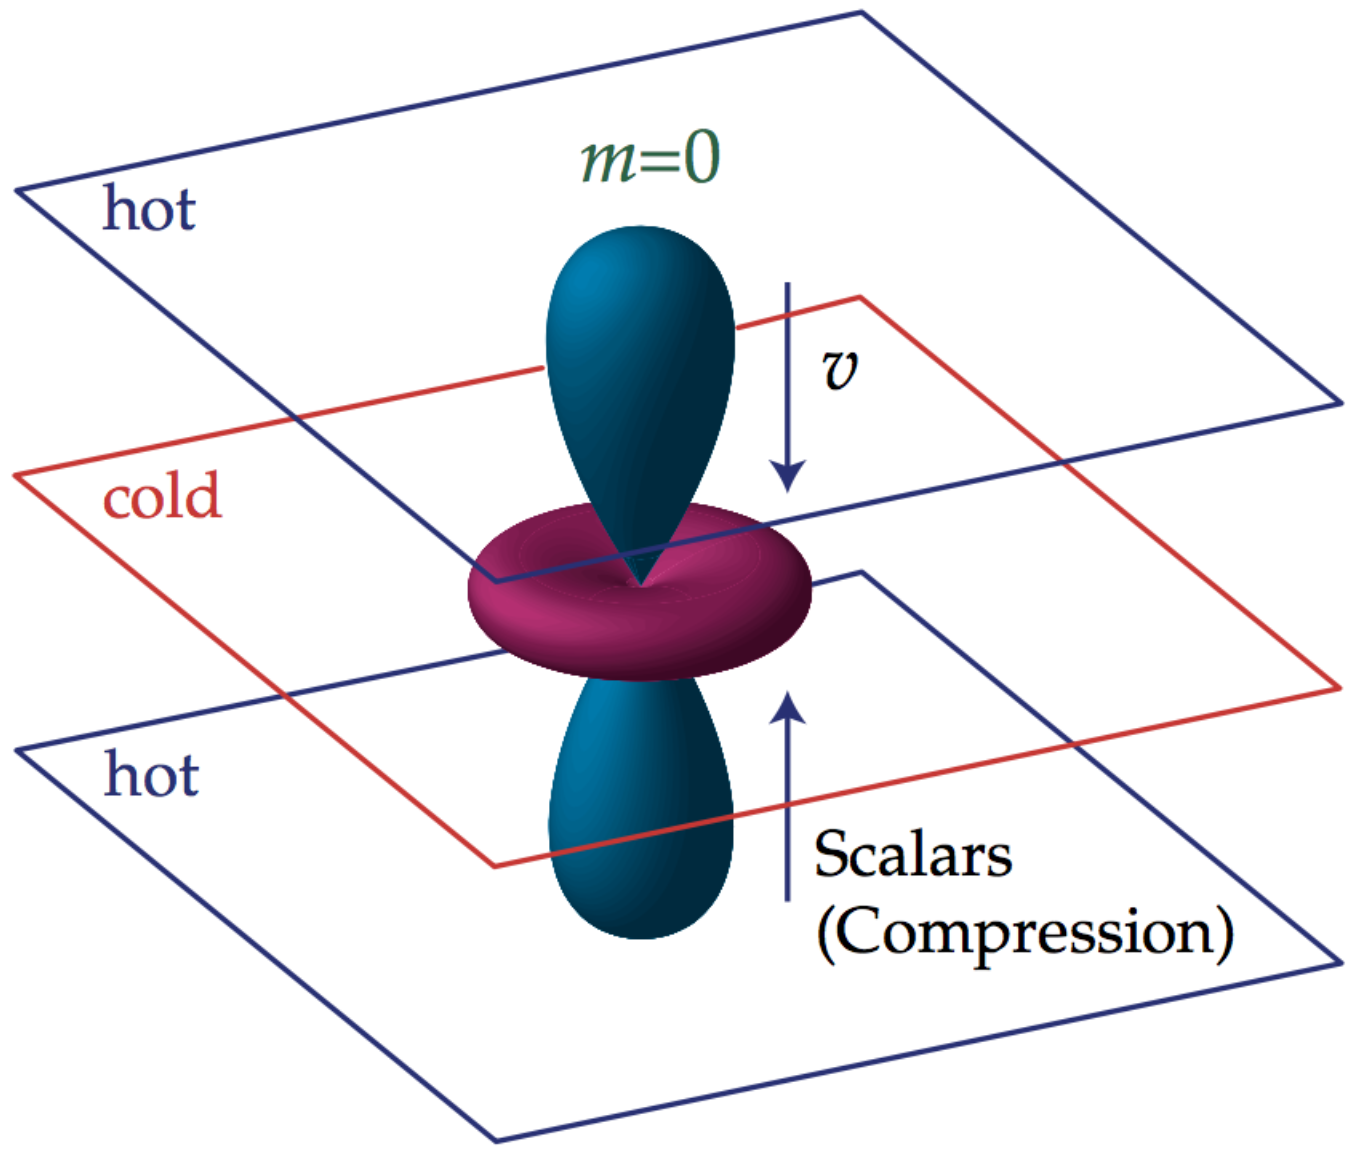
\includegraphics[width=8cm]{figures/ScalarQuadrupole.png}\\
    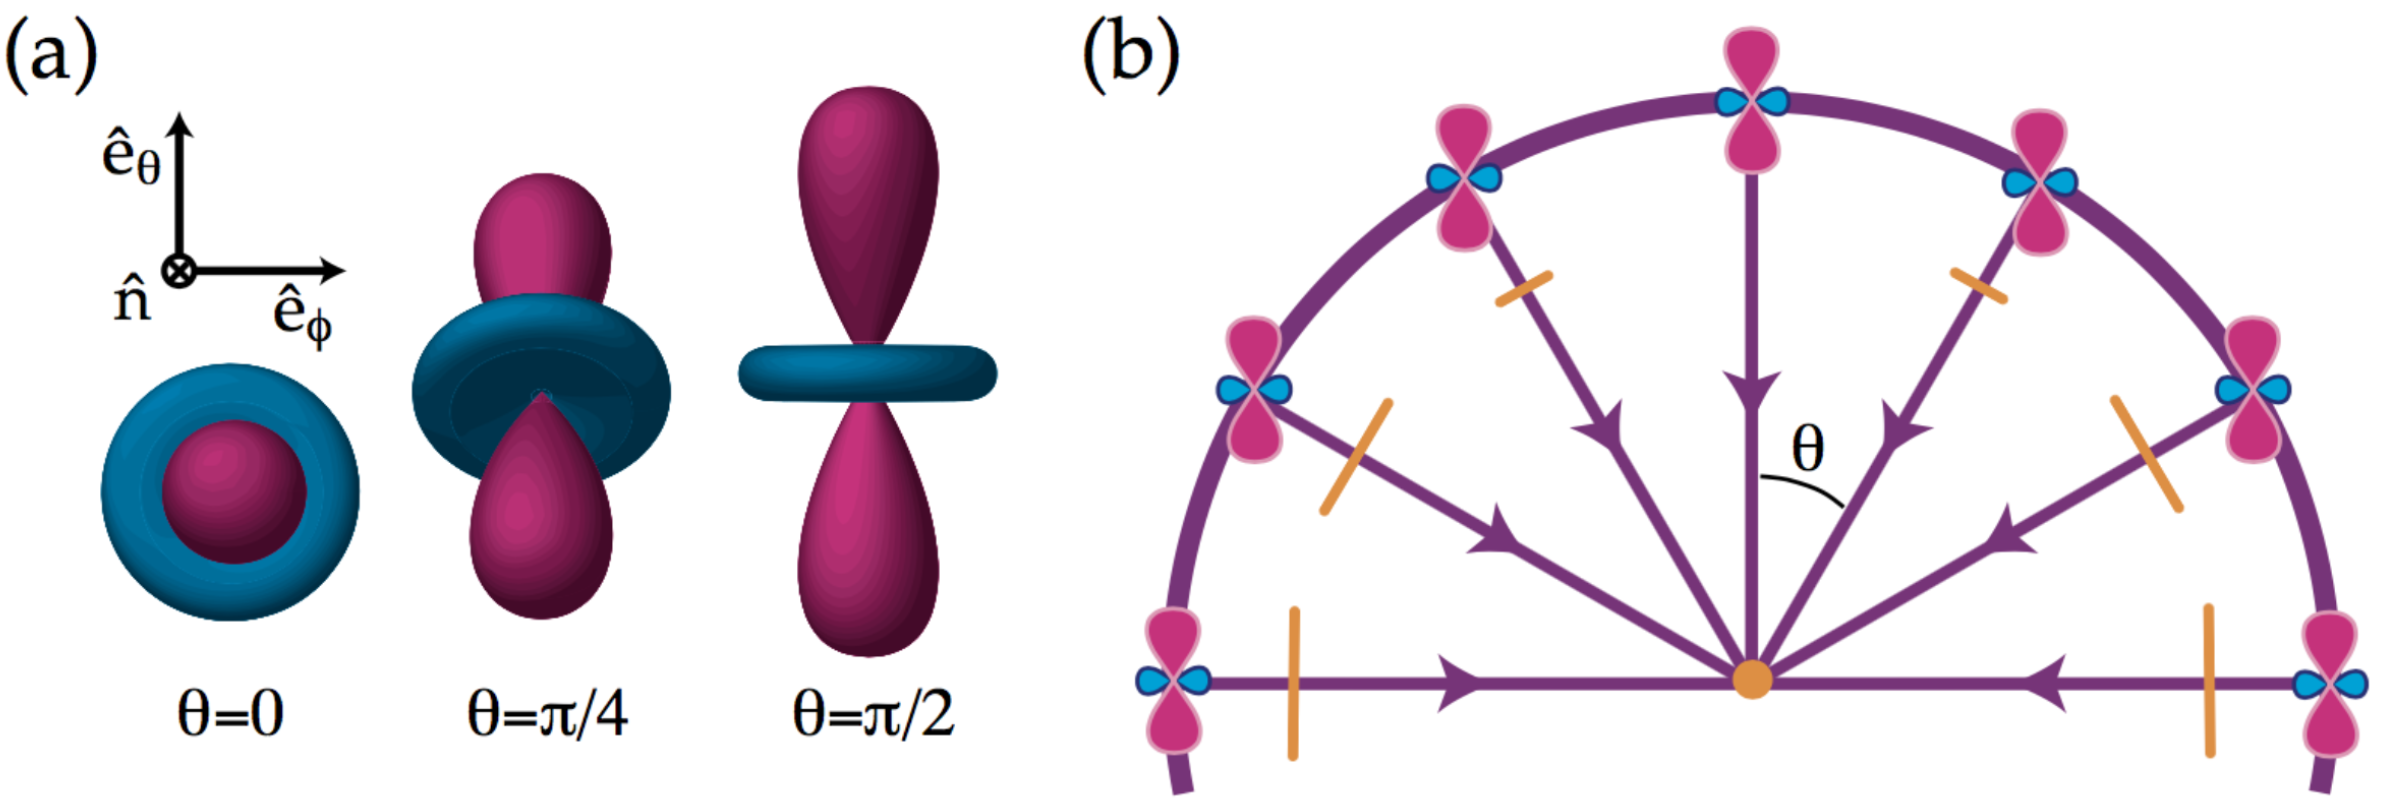
\includegraphics[width=15cm]{figures/QuadrupolarAnisotropies.png}\\
    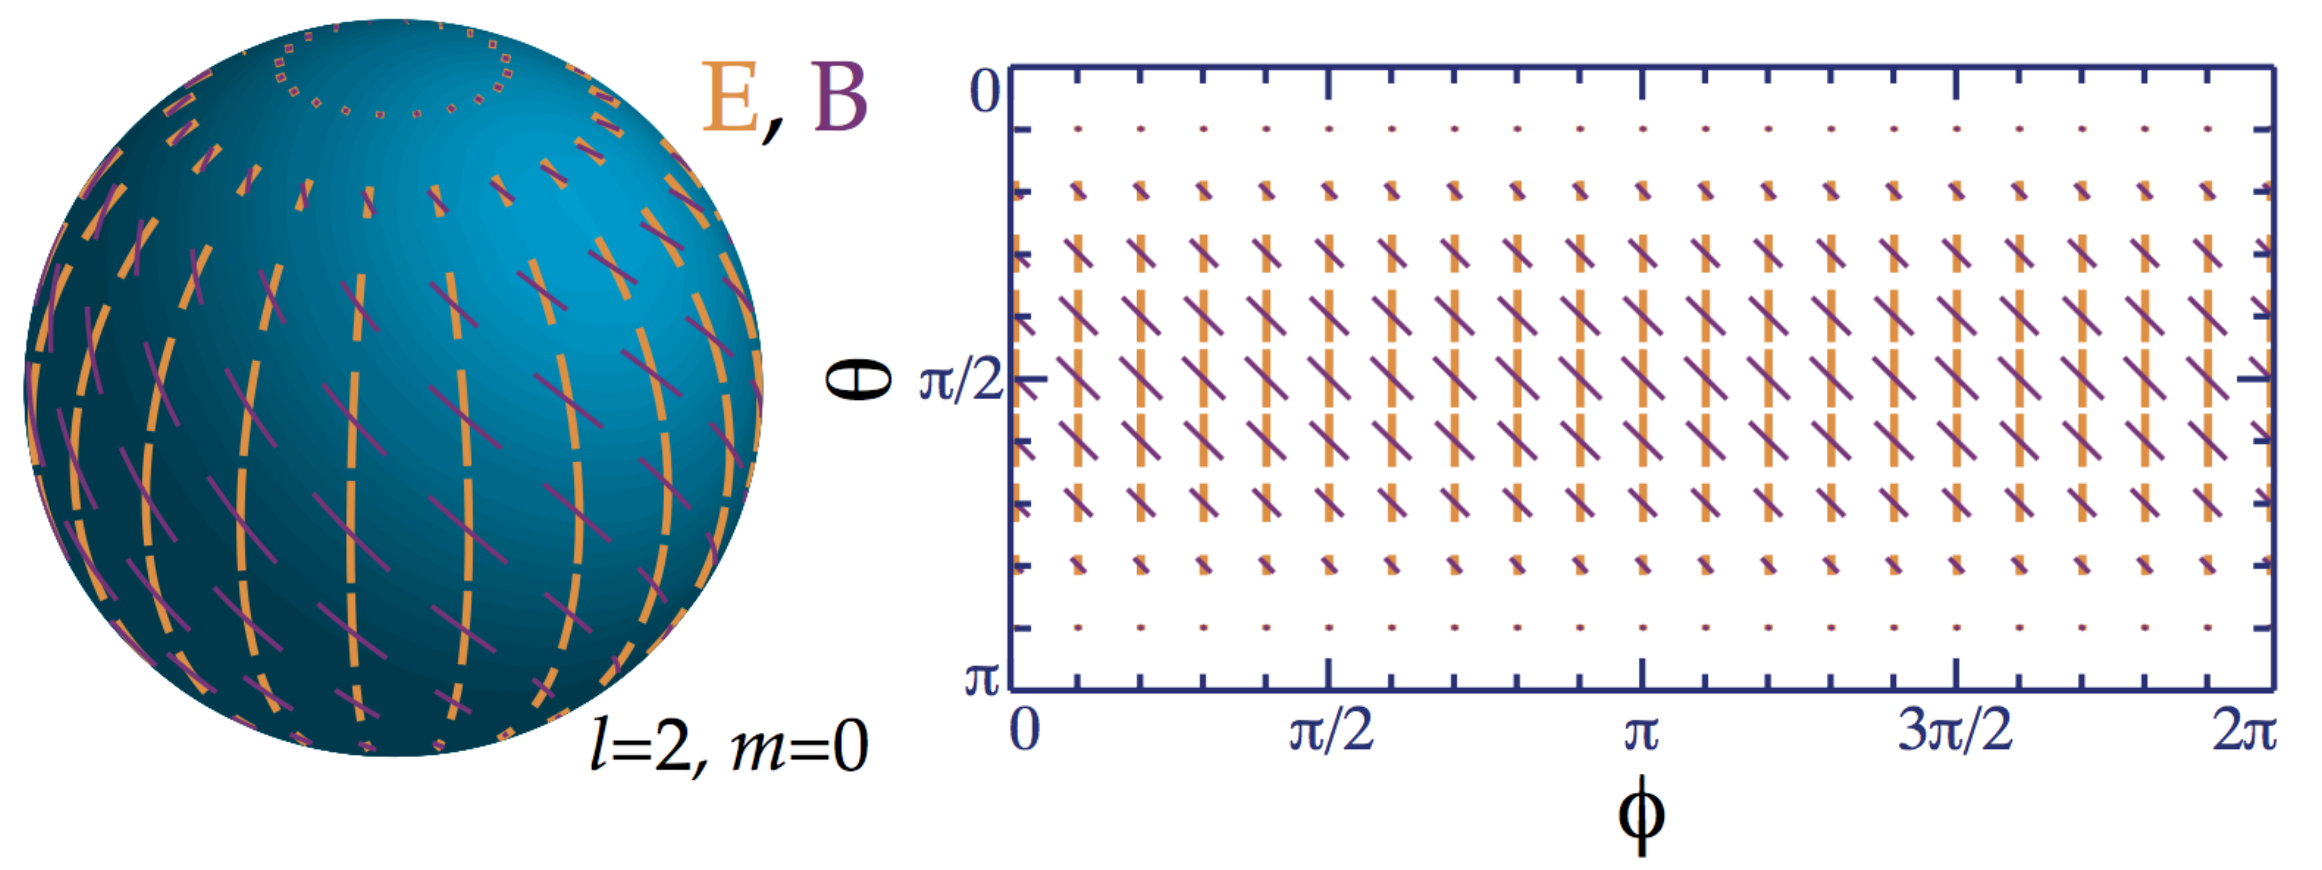
\includegraphics[width=15cm]{figures/ScalarPattern.png}
    \caption{\footnotesize{\textbf{(Top)} The scalar quadrupole moment ($\ell=2,m=0$). Flows from hot (blue) regions into cold (red), $\bm{v}\parallel\bm{k}$, produce the azimuthally symmetric pattern $Y_2^0$ depicted here. \textbf{(Middle)} The transformation of quadrupole anisotropies into linear polarization. (a) The orientation of the quadrupole moment with respect to the scattering direction $\bm{\hat{n}}$ determines the sense and magnitude of the polarization. It is aligned with the cold (red, long) lobe in the $\bm{\hat{e}}_\theta\times\bm{\hat{e}}_\phi$ tangent plane. (b) In spherical coordinates where $\bm{\hat{n}}\cdot\bm{\hat{k}}=\cos\theta$, the polarization points north-south ($Q$) with magnitude varying as $\sin^2θ$ for scalar fluctuations. \textbf{(Bottom)} Polarization pattern for $\ell=2,m=0$, note the azimuthal symmetry. The scattering of a scalar $m=0$ quadrupole perturbation generates the electric $E$ (yellow, thick lines) pattern on the sphere. Its rotation by $45^\circ$ represents the orthogonal magnetic $B$ (purple, thin lines) pattern. Animation (available at \href{http://www.sns.ias.edu/∼whu/polar/scalaran.html}{http://www.sns.ias.edu/∼whu/polar/scalaran.html}): as the line of sight $\bm{\hat{n}}$ changes, the lobes of the quadrupole rotate in and out of the tangent plane. The polarization follows the orientation of the colder (red) lobe in the tangent plane. Images taken from Hu \& White (1997).}}
    \label{fig:scalar}
\end{figure}

{\noindent}Let us consider the quadrupole component of the temperature pattern seen by an observer located in a trough of a plane wave. The azimuthal symmetry in the problem requires that $\bm{v}\parallel\bm{k}$ and hence the flow is irrotational $\nabla\times\bm{v}=0$. Because hotter photons from the crests flow into the trough from the $\pm k$ directions while cold photons surround the observer in the plane, the quadrupole pattern seen in a trough has an $m = 0$,

\begin{align*}
    Y_2^0 \propto 3\cos^2\theta-1,
\end{align*}

{\noindent}structure with angle $\bm{\hat{n}\cdot\hat{k}}=\cos\theta$ (see top of Figure \ref{fig:scalar}). The opposite effect occurs at the crests, reversing the sign of the quadrupole but preserving the $m=0$ nature in its local angular dependence. The full effect is thus described by a local quadrupole modulated by a plane wave in space, $-Y_2^0(\bm{\hat{n}})\exp(i\bm{k}\cdot\bm{x})$, where the sign denotes the fact that photons flowing into cold regions are hot. This infall picture must be modified slightly on scales smaller than the sound horizon where pressure plays a role, however the essential property that the flows are parallel to $\bm{\hat{k}}$ and thus generate an $m=0$ quadrupole remains true.

{\noindent}The sense of the quadrupole moment determines the polarization pattern through Thomson scattering. Recall that polarized scattering peaks when the temperature varies in the direction orthogonal to $\bm{\hat{n}}$. Consider then the tangent plane $\bm{\hat{e}}_\theta\times\bm{\hat{e}}_\phi$ with normal $\bm{\hat{n}}$. This may be visualized in an angular ``lobe'' diagram such as the top of Figure \ref{fig:scalar} as a plane which passes through the ``origin'' of the quadrupole pattern perpendicular to the line of sight. The polarization is maximal when the hot and cold lobes of the quadrupole are in this tangent plane, and is aligned with the component of the colder lobe which lies in the plane. As $\theta$ varies from $0$ to $\pi/2$ (pole to equator) the temperature differences in this plane increase from zero (see middle of Figure \ref{fig:scalar} a). The local polarization at the crest of the temperature perturbation is thus purely in the N-S direction tapering off in amplitude toward the poles (see middle of Figure \ref{fig:scalar} b). This pattern represents a pure $Q$-field on the sky whose amplitude varies in angle as an $\ell=2,m=0$ tensor or spin-$2$ spherical harmonic (Newman \& Penrose, 1966)

\begin{align*}
    Q=\sin^2\theta,~~~~~U=0.
\end{align*}

{\noindent}In different regions of space, the plane wave modulation of the quadrupole can change the sign of the polarization, but not its sense.

{\noindent}This pattern (bottom of Figure \ref{fig:scalar}, thick lines) is of course not the only logical possibility for an $\ell=2,m=0$ polarization pattern. Its rotation by $45^\circ$ is also a valid configuration (thin lines). This represents a pure NW-SE (and by sign reversal NE-SW), or $U$-polarization pattern (a distinction between the two patterns being electric and magnetic modes).

{\noindent}\textbf{Vector (vortical) perturbations}:

{\noindent}Vector perturbations represent vortical motions of the matter, where the velocity field $\bm{v}$ obeys $\nabla\cdot\bm{v}=0$ and $\nabla\times\bm{v}\neq0$, similar to ``eddies'' in water. There is no associated density perturbation, and the vorticity is damped by the expansion of the Universe as are all motions that are not enhanced by gravity. However, the associated temperature fluctuations, once generated, do not decay as both $\Delta T$ and $T$ scale similarly with the expansion. For a plane wave perturbation, the velocity field $\bm{v}\perp\bm{k}$ with direction reversing in crests and troughs (see top of Figure \ref{fig:vector}). The radiation field at these extrema possesses a dipole pattern due to the Doppler shift from the bulk motion. Quadrupole variations vanish here but peak between velocity extrema. To see this, imagine sitting between crests and troughs. Looking up toward the trough, one sees the dipole pattern projected as a hot and cold spot across the zenith; looking down toward the crest, one sees the projected dipole reversed. The net effect is a quadrupole pattern in temperature with $m\pm1$

\begin{align*}
    Y_2^{\pm1}\propto\sin\theta\cos\theta\mathrm{e}{\pm i\phi}.
\end{align*}

\begin{figure}[t!]
    \centering
    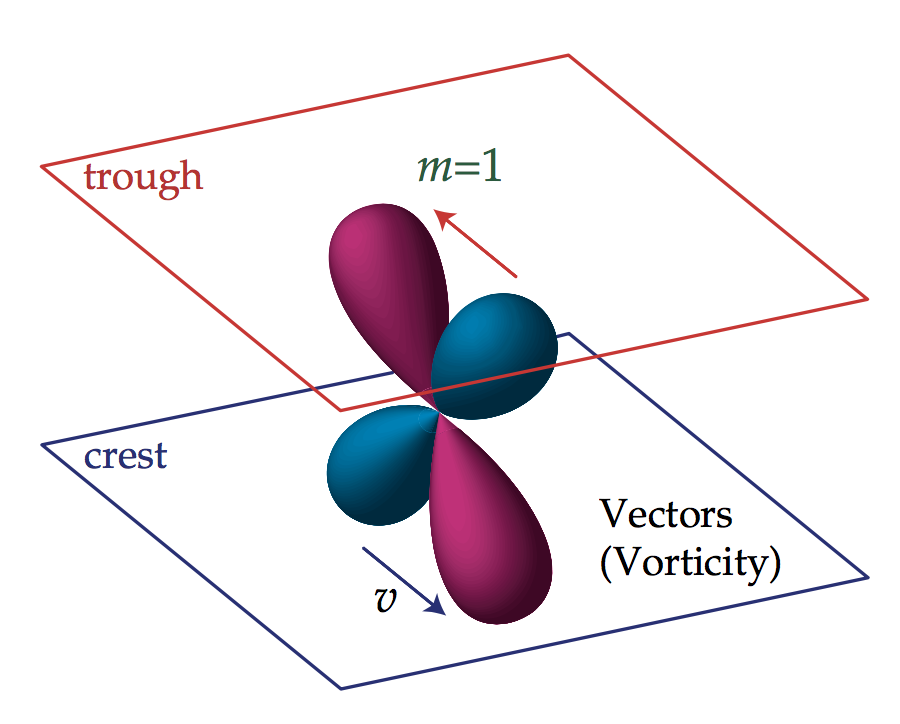
\includegraphics[width=8cm]{figures/VectorQuadrupole.png}
    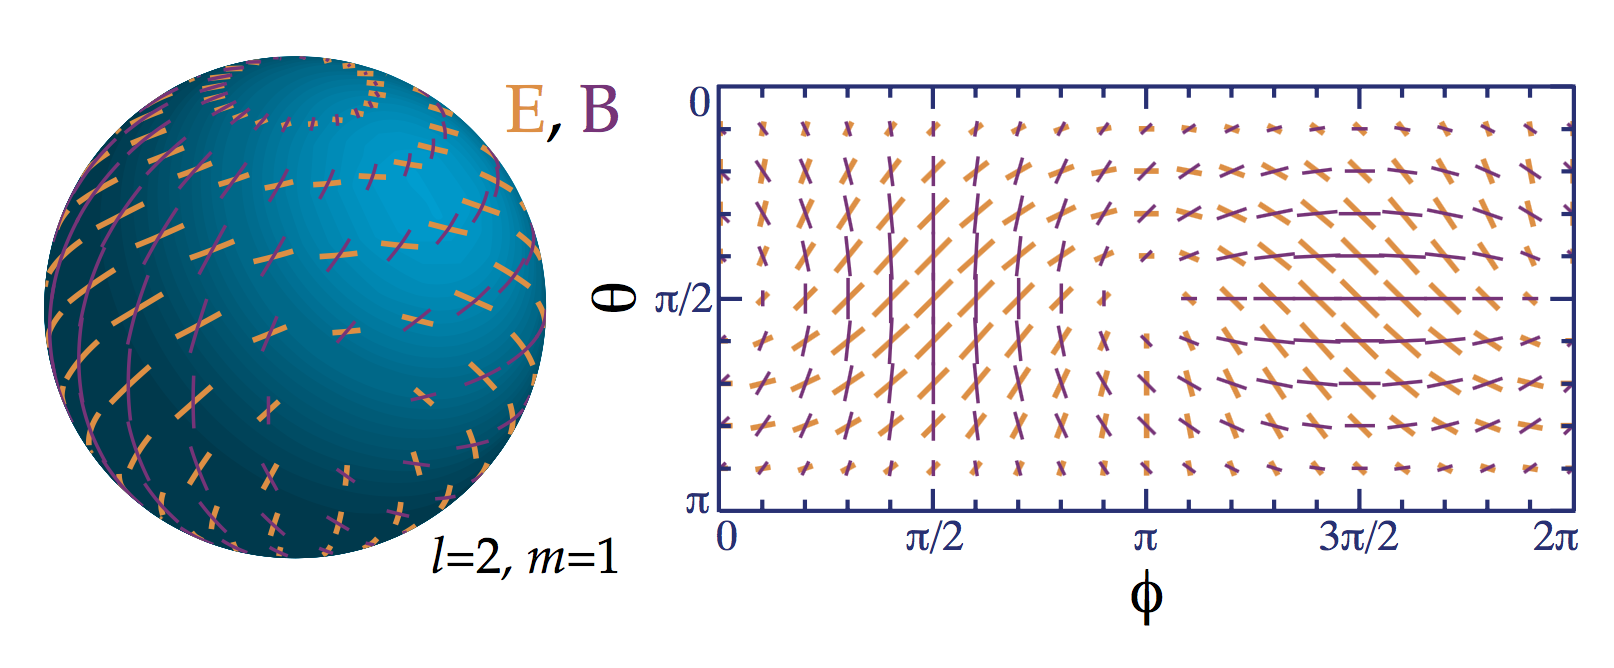
\includegraphics[width=15cm]{figures/VectorPattern.png}
    \caption{\footnotesize{\textbf{(Top)} The vector quadrupole moment ($l=2,m=1$). Since $\bm{v}\perp\bm{k}$, the Doppler effect generates a quadrupole pattern with lobes $45^\circ$ from $\bm{v}$ and $\bm{k}$ that is spatially out of phase (interplane peaks) with $v$. \textbf{(Bottom)} Polarization pattern for $\ell=2,m=1$. The scattering of a vector ($m=1$) quadrupole perturbation generates the $E$ pattern (yellow, thick lines) as opposed to the $B$, (purple, thin lines) pattern. Animation (available at \href{http://www.sns.ias.edu/∼whu/polar/vectoran.html}{http://www.sns.ias.edu/∼whu/polar/vectoran.html}): same as for scalars. Images taken from Hu \& White (1997).}}
    \label{fig:vector}
\end{figure}

{\noindent}The lobes are oriented at $45^\circ$ from $k$ and $v$ since the line
of sight velocity vanishes along $k$ and at $90$ degrees to $k$ here. The latter follows since midway between the crests and troughs $v$ itself is zero. The full quadrupole distribution is therefore described by $-iY_2^{\pm1}(\bm{\hat{n}})\exp(i\bm{k}\cdot\bm{x})$, where $i$ represents the spatial phase shift of the quadrupole with respect to the velocity.

{\noindent}Thomson scattering transforms the quadrupole temperature anisotropy into a local polarization field as before. Again, the pattern may be visualized from the intersection of the tangent plane to $\bm{\hat{n}}$ with the lobe pattern of the top of Figure \ref{fig:vector}. At the equator ($\theta=\pi/2$), the lobes are oriented $45^\circ$ from the line of sight $\bm{\hat{n}}$ and rotate into and out of the tangent plane with $\phi$. The polarization pattern here is a pure $U$-field which varies in magnitude as $\sin\phi$. At the pole $\theta=0$, there are no temperature variations in the tangent plane so the polarization vanishes. Other angles can equally well be visualized by viewing the quadrupole pattern at different orientations given by $\bm{\hat{n}}$.

{\noindent}The full $\ell=2,m=1$ pattern,

\begin{align*}
    Q=-\sin\theta\cos\theta\mathrm{e}^{i\phi},~~~~~U=-i\sin\theta\mathrm{e}^{i\phi}
\end{align*}

{\noindent}is displayed explicitly in the bottom of Figure \ref{fig:vector}. Note that the pattern is dominated by $U$-contributions especially near the equator.

{\noindent}\textbf{Tensor (gravitational wave) perturbations}:

{\noindent}Tensor fluctuations are transverse-traceless perturbations to the metric, which can be viewed as gravitational waves. A plane gravitational wave perturbation represents a quadrupolar ``stretching'' of space in the plane of the perturbation (see Figure \ref{fig:tensorquadrupole}). As the wave passes or its amplitude changes, a circle of test particles in the plane is distorted into an ellipse whose semi-major axis $\rightarrow$ semi-minor axis as the spatial phase changes from crest $\rightarrow$ trough (see the top of Figure \ref{fig:tensor}, yellow ellipses). Heuristically, the accompanying stretching of the wavelength of photons produces a quadrupolar temperature variation with an $m=\pm2$ pattern

\begin{align*}
    Y_2^{\pm2}\propto\sin^2\theta\mathrm{e}^{\pm2i\phi}
\end{align*}

{\noindent}in the coordinates defined by $\bm{\hat{k}}$.

\begin{figure}[t!]
    \centering
    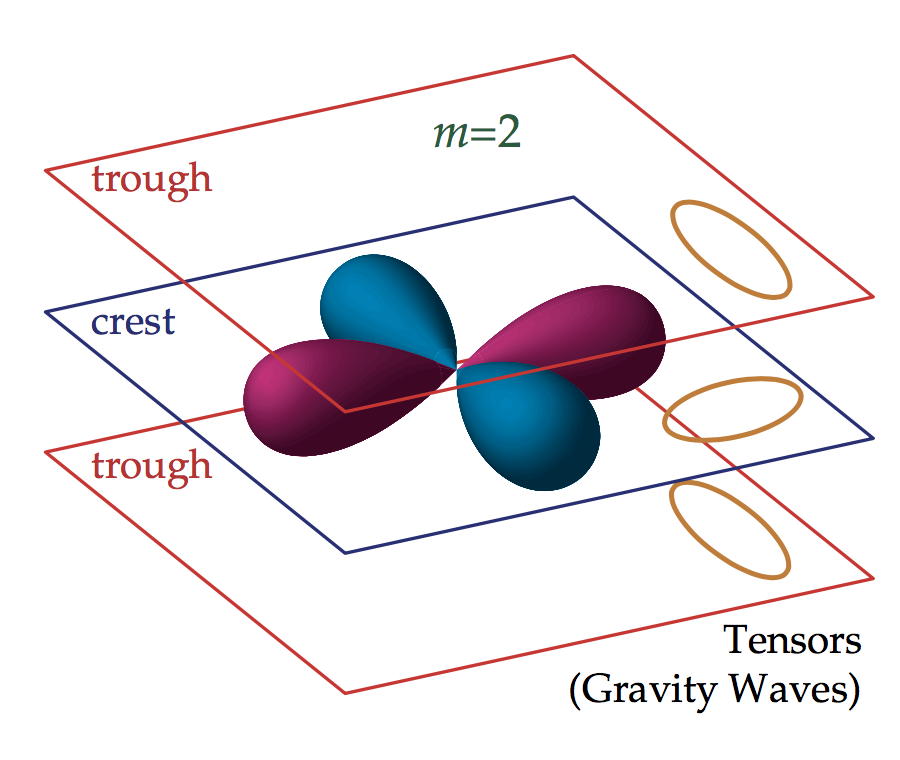
\includegraphics[width=8cm]{figures/TensorQuadrupole.png}
    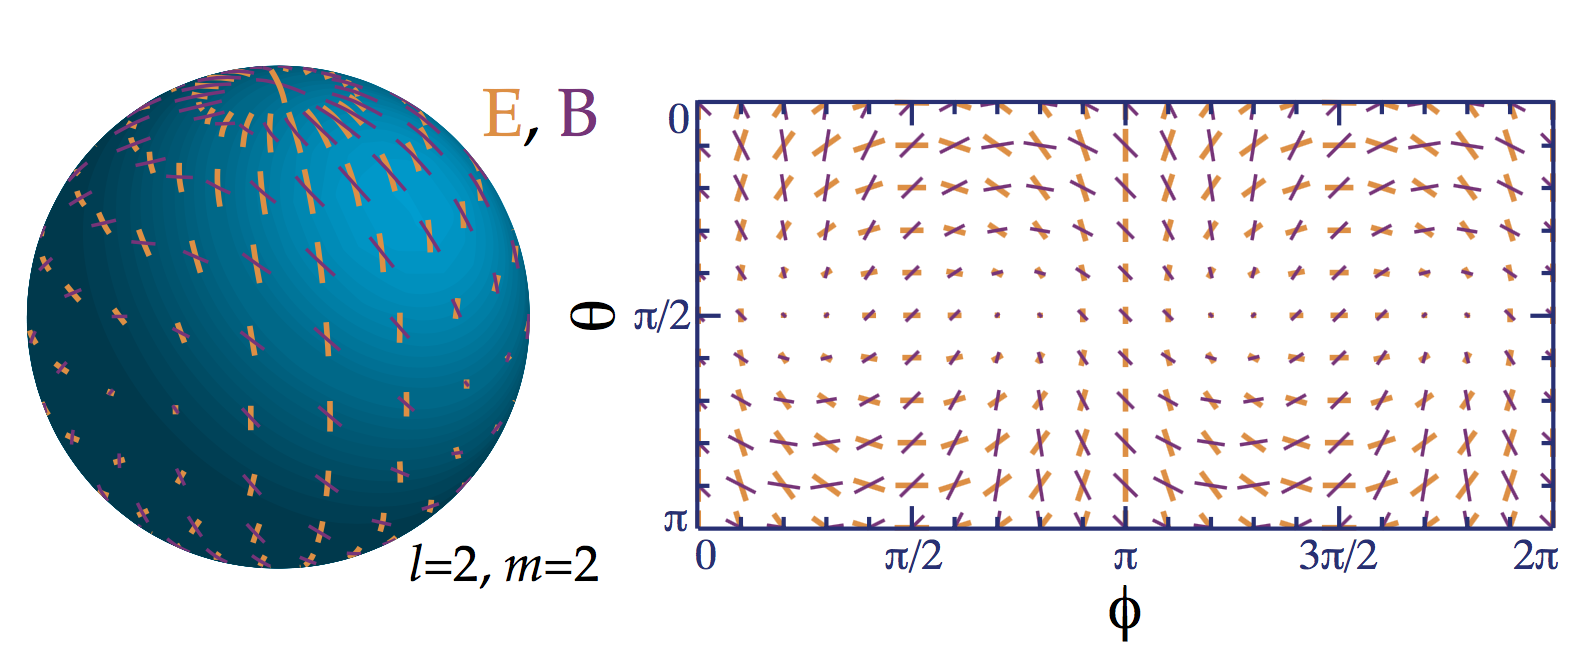
\includegraphics[width=15cm]{figures/TensorPattern.png}
    \caption{\footnotesize{\textbf{(Top)} The tensor quadrupole moment $(m=2)$. Since gravity waves distort space in the plane of the perturbation, changing a circle of test particles into an ellipse, the radiation acquires an $m=2$ quadrupole moment. \textbf{(Bottom)} Polarization pattern for $\ell=2,m=2$. Scattering of a tensor $m=2$ perturbation generates the $E$ (yellow, thick lines) pattern as opposed to the $B$ (purple, thin lines) pattern. Animation (available at \href{http://www.sns.ias.edu/∼whu/polar/vectoran.html}{http://www.sns.ias.edu/∼whu/polar/vectoran.html}): same as for scalars. Images taken from Hu \& White (1997).}}
    \label{fig:tensor}
\end{figure}

{\noindent}Thomson scattering again produces a polarization pattern from the quadrupole anisotropy. At the equator, the quadrupole pattern intersects the tangent ($\bm{\hat{e}}_\theta\times\bm{\hat{e}}_\phi$) plane with hot and cold lobes rotating in and out of the $\bm{\hat{e}}_\phi$ direction with the azimuthal angle $\phi$. The polarization pattern is therefore purely $Q$ with a $\cos(2\phi)$ dependence. At the pole, the quadrupole lobes lie completely in the polarization plane and produces the maximal polarization unlike the scalar and vector cases. The full pattern,

\begin{align*}
    Q=(1+\cos^2\theta)\mathrm{e}^{2i\phi}~[{\rm Jy}], ~~~~~U=-2i\cos\theta\mathrm{e}^{2i\phi}~[{\rm Jy}],
\end{align*}

{\noindent}is shown in the bottom of Figure \ref{fig:tensor} (real part). Note that $Q$ and $U$ are present in nearly equal amounts for the tensors.

{\noindent}\textit{Electric and Magnetic Modes}:

{\noindent}Any polarization pattern on the sky can be separated into ``electric'' ($E$) and ``magnetic'' ($B$) components. This decomposition is useful both observationally and theoretically. There are two equivalent ways of viewing the modes that reflect their global and local properties respectively. The nomenclature reflects the global property. Like multipole radiation, the harmonics of an $E$-mode have $(-1)^\ell$ parity on the sphere, whereas those of a $B$-mode have $(-1)^{\ell+1}$ parity. Under $\bm{\hat{n}}\rightarrow\bm{\hat{n}}$, the $E$-mode thus remains unchanged for even $\ell$, whereas the $B$-mode changes sign as illustrated for the simplest case $\ell=2,m=0$ in Figure \ref{fig:ebmodes} (recall that a rotation by $90^\circ$ represents a change in sign). Note that the $E$ and $B$ multipole patterns are $45^\circ$ rotations of each other, (i.e. $Q\rightarrow U$ and $U\rightarrow-Q$). Since this parity property is obviously rotationally invariant, it will survive integration over $\bm{\hat{k}}$.

{\noindent}The local view of $E$- and $B$-modes involves the second derivatives of the polarization amplitude (second derivatives because polarization is a tensor or spin-$2$ object). In much the same way that the distinction between electric and magnetic fields in electromagnetism involves vanishing of gradients or curls (i.e., first derivatives) for the polarization there are conditions on the second (covariant) derivatives of $Q$ and $U$. For an $E$-mode, the difference in second (covariant) derivatives of $U$ along $\bm{\hat{e}}_\theta$ and $\bm{\hat{e}}_\phi$ vanishes as does that for $Q$ along $\bm{\hat{e}}_\theta+\bm{\hat{e}}_\phi$ and $\bm{\hat{e}}_\theta-\bm{\hat{e}}_\phi$. For a $B$-mode, $Q$ and $U$ are interchanged. Recalling that a $Q$-field points in the $\bm{\hat{e}}_\theta$ or $\bm{\hat{e}}_\phi$ direction and a $U$-field in the crossed direction, we see that the Hessian or curvature matrix of the polarization amplitude has principle axes in the same sense as the polarization for $E$ and $45^\circ$ crossed with it for $B$ (see Figure \ref{fig:ebmodes}). Stated another way, near a maximum of the polarization (where the first derivative vanishes) the direction of greatest change in the polarization is parallel/perpendicular and at $45^\circ$ degrees to the polarization in the two cases.

{\noindent}The distinction is best illustrated with examples. Take the simplest case of $\ell=2,m=0$ where the $E$-mode is a $Q=\sin^2\theta$ field and the $B$-mode is a $U=\sin^2\theta$ field (see the bottom of Figure \ref{fig:scalar}). In both cases, the major axis of the curvature lies in the $\bm{\hat{e}}_\theta$ direction. For the $E$-mode, this is in the same sense; for the $B$-mode it is crossed with the polarization direction. The same holds true for the $m=1,2$ modes as can be seen by inspection of the bottom of Figure \ref{fig:vector} and the bottom of Figure \ref{fig:tensor}.

\begin{figure}[t!]
    \centering
    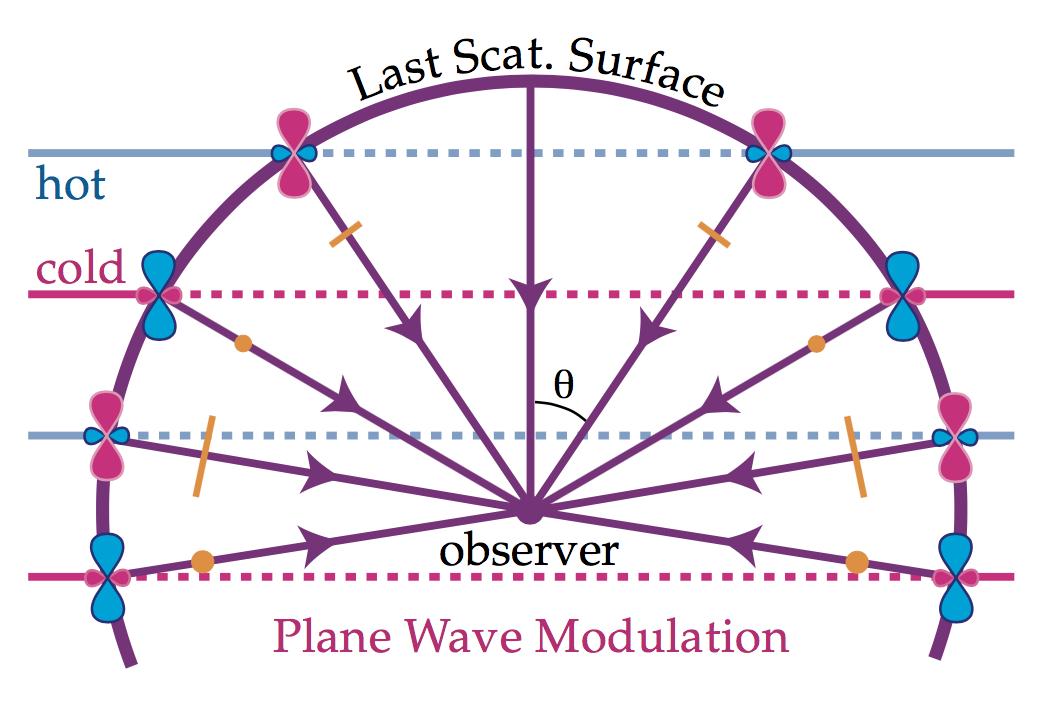
\includegraphics[width=10cm]{figures/CMBquad.png}
    \caption{\footnotesize{Modulation of the local pattern in the bottom of Figure \ref{fig:scalar} by plane wave fluctuations on the last scattering surface. Yellow points represent polarization out of the plane with magnitude proportional to sign. The plane wave modulation changes the amplitude and sign of the polarization but does not mix $Q$ and $U$. Modulation can mix $E$ and $B$ however if $U$ is also present. Image taken from Hu \& White (1997).}}
    \label{fig:cmbquad}
\end{figure}

{\noindent}Thomson scattering can only produce an $E$-mode locally since the spherical harmonics that describe the temperature anisotropy have $(-1)^\ell$ electric parity. In the tops of Figures \ref{fig:scalar}, \ref{fig:vector}, and \ref{fig:tensor}, the $\ell=2,m=0,1,2$ $E$-mode patterns are shown in yellow. The $B$-mode represents these patterns rotated by $45^\circ$ and are shown in purple and cannot be generated by scattering. In this way, the scalars, vectors, and tensors are similar in that scattering produces a local $\ell=2$ $E$-mode only.

{\noindent}However, the pattern of polarization on the sky is not simply this local signature from scattering but is modulated over the last scattering surface by the plane wave spatial dependence of the perturbation (compare the bottom of Figure \ref{fig:scalar} and \ref{fig:cmbquad}). The modulation changes the amplitude, sign, and angular structure of the polarization but not its nature, e.g. a $Q$-polarization remains Q. Nonetheless, this modulation generates a $B$-mode from the local $E$-mode pattern.

{\noindent}The reason why this occurs is best seen from the local distinction between $E$ and $B$-modes. Recall that $E$-modes have polarization amplitudes that change parallel or perpendicular to, and $B$-modes in directions $45^\circ$ away from, the polarization direction. On the other hand, plane wave modulation always changes the polarization amplitude in the direction $\bm{\hat{k}}$ or N-S on the sphere. Whether the resultant pattern possesses $E$ or $B$-contributions depends on whether the local polarization has $Q$ or $U$-contributions.

{\noindent}For scalars, the modulation is of a pure $Q$-field and thus its $E$-mode nature is preserved (Kamionkowski et al. 1997; Zaldarriaga \& Seljak 1997). For the vectors, the $U$-mode dominates the pattern and the modulation is crossed with the polarization direction. Thus vectors generate mainly $B$-modes for short wavelength fluctuations (Hu \& White 1997). For the tensors, the comparable $Q$ and $U$ components of the local pattern imply a more comparable distribution of $E$ and $B$ modes at short wavelengths (see Figure \ref{fig:polpatterns}a).

\begin{figure}[t!]
    \centering
    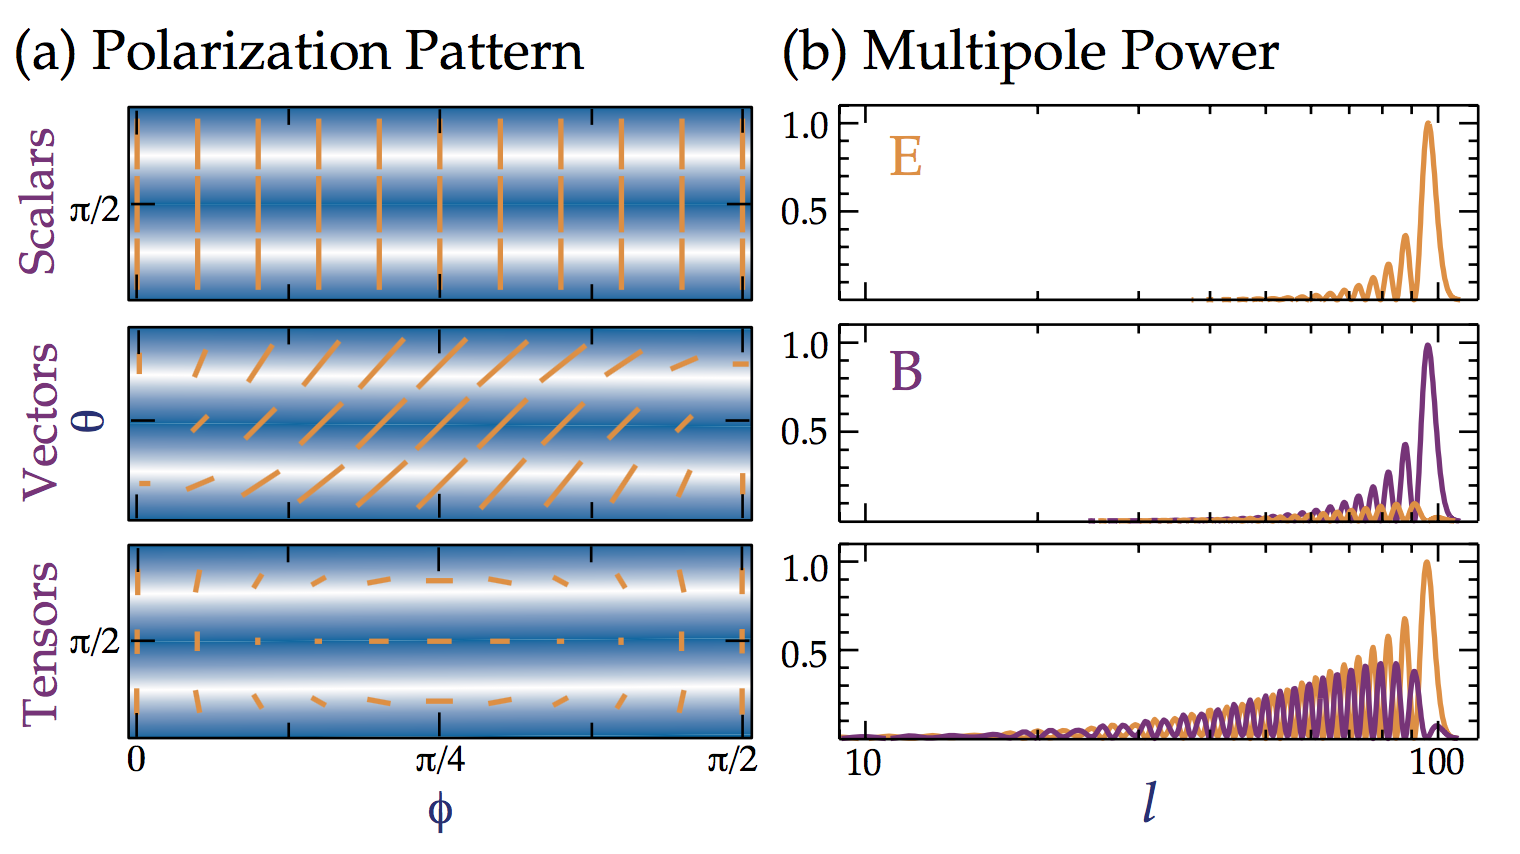
\includegraphics[width=16cm]{figures/PolPatterns.png}
    \caption{\footnotesize{The $E$ and $B$ components of a plane wave perturbation. (a) Modulation of the local $E$-quadrupole pattern (yellow) from scattering by a plane wave. Modulation in the direction of (or orthogonal to) the polarization generates an $E$-mode with higher $\ell$; modulation in the crossed ($45^\circ$) direction generates a $B$-mode with higher $\ell$. Scalars generate only $E$-modes, vectors mainly $B$-modes, and tensors comparable amounts of both. (b) Distribution of power in a single plane wave with $kr=100$ in multipole $\ell$ from the addition of spin and orbital angular momentum. Features in the power spectrum can be read directly off the pattern in (a). Image taken from Hu \& White (1997).}}
    \label{fig:polpatterns}
\end{figure}

{\noindent}These qualitative considerations can be quantified by noting that plane wave modulation simply represent the addition of angular momentum from the plane wave ($Y_\ell^0$) with the local spin angular dependence. The result is that plane wave modulation takes the $\ell=2$ local angular dependence to higher $\ell$ (smaller angles) and splits the signal into $E$ and $B$ components with ratios which are related to Clebsch-Gordan coefficients. At short wavelengths, these ratios are $B/E=0$, $6$, $8/13$ in power for scalars, vectors, and tensors (see Figure \ref{fig:polpatterns}b and Hu \& White 1997).

{\noindent}The distribution of power in multipole $\ell$-space is also important. Due to projection, a single plane wave contributes to a range of angular scales  $\ell\lesssim kr$ where $r$ is the comoving distance to the last scattering surface. From Figure \ref{fig:cmbquad}, we see that the smallest angular, largest $\ell\approx kr$ variations occur on lines of sight $\bm{\hat{n}}\cdot\bm{\hat{k}}=0$ or $\theta=\pi/2$ though a small amount of power projects to $\ell\ll kr$ as $\theta\rightarrow0$. The distribution of power in multipole space of Figure \ref{fig:polpatterns}b can be read directly off the local polarization pattern. In particular, the region near $\theta=\pi/2$ shown in Figure \ref{fig:polpatterns}a determines the behavior of the main contribution to the polarization power spectrum.

{\noindent}The full power spectrum is of course obtained by summing these plane wave contributions with weights dependent on the source of the perturbations and the dynamics of their evolution up to last scattering. Sharp features in the $k$-power spectrum will be preserved in the multipole power spectrum to the extent that the projectors in Figure \ref{fig:polpatterns}b approximate delta functions. For scalar $E$-modes, the sharpness of the projection is enhanced due to strong $Q$-contributions near $\theta=\pi/2$ $(\ell\sim kr)$ that then diminish as $\theta\rightarrow0$ $(\ell\ll kr)$. The same enhancement occurs to a lesser extent for vector $B$-modes due to $U$ near $\pi/2$ and tensor $E$-modes due to $Q$ there. On the other hand, a suppression occurs for vector $E$ and tensor $B$-modes due to the absence of $Q$ and $U$ at $\pi/2$ respectively. These considerations have consequences for the sharpness of features in the polarization power spectrum, and the generation of asymptotic ``tails'' to the polarization spectrum at low-$\ell$ (see Hu \& White 1997) .

% --------------------------------------------------------------
%
%                           18. 
%
% --------------------------------------------------------------

\newpage
\subsection{Question 18}

What are the similarities and differences between the cosmic neutrino background and the cosmic microwave background?

\subsubsection{Short answer}

Just as the CMB is a relic of the time when the Universe was opaque to photons, the CNB is a relic of the time when the Universe was hot and dense enough to be opaque to neutrinos.

{\noindent}The number density of each of the three flavors of neutrinos ($\nu_e$, $\nu_\mu$, and $\nu_\tau$) has been calculated to be 3/11 times the number density of CMB photons. This means that at any moment, about twenty million cosmic neutrinos are zipping through your body.

\subsubsection{Additional context}

Additional context.

\subsubsection{Follow-up Questions}

\begin{itemize}
    \item What is a neutrino?
    \item How do we determine their mass?
    \item Besides the sun and the CNB, what other sources of neutrinos are there?
    \item What is the neutrino contribution to the density of the Universe?
    \item Why do neutrinos decouple at 1 second (i.e., before photons)?
\end{itemize}


% --------------------------------------------------------------
%
%                           19. 
%
% --------------------------------------------------------------

\newpage
\subsection{Question 19}

What is the difference between an isocurvature mode and an adiabatic mode, in terms of the initial density perturbations in the early universe? How do we know that the initial conditions are mostly adiabatic?

\subsubsection{Short answer}

Answer.

\subsubsection{Additional context}

In a complete description of energy density perturbations, the total energy density of the Universe includes components of baryonic matter ($\rho_b$), dark matter ($\rho_c$), radiation ($\rho_\mathrm{rad}$), and dark energy ($\rho_\Lambda$):

\begin{align*}
    \rho(\mathbf{x},t) = \rho_b(\mathbf{x},t) + \rho_c(\mathbf{x},t) + \rho_\mathrm{rad}(\mathbf{x},t) + \rho_\Lambda(\mathbf{x},t).
\end{align*}

{\noindent}In terms of their global gravitational influence, dark matter and baryonic matter contribute and evolve equivalently, therefore on cosmological scales they can be combined into a total matter energy density $\rho_m = \rho_b + \rho_c$. Each component may have its own (primordial) perturbation character. Dark energy does not have any density fluctuations, so $\delta_\Lambda(\mathbf{x},t) = 0$. Since most of the structure formation happened during the \textit{matter-dominated era}, this mainly involves the evolution of matter linear perturbations $\delta_m(\mathbf{x},t)$.

{\noindent}Cosmological perturbations will evolve quite differently for different \textit{perturbation modes}, each of which are identified on the basis of the nature of radiation perturbations with respect to matter perturbations. \textit{Isothermal perturbation modes} only involve matter perturbations ($\delta_m$) while radiation remains uniformly distributed throughout the 
Universe ($\delta_\mathrm{rad} = 0$). On the other hand, the primordial perturbations $\delta_m$ and $\delta_\mathrm{rad}$ may be completely equivalent (except for a constant proportionality factor) corresponding to zero fluctuations in entropy; these are \textit{adiabatic perturbation modes}. A third type of perturbation is that of \textit{isocurvature perturbation modes} in which radiation and matter perturbations cancel each other out such that the local curvature remains equal to the global cosmological curvature. Moreover, the evolution of the various components is complicated to a considerable extent by their mutual interactions. A simple illustration is that of baryonic matter initially without density perturbations: while dark matter creates even deeper potential wells, baryonic matter will fall in and experience increasingly stronger perturbations. Also, in pre-recombination epoch, baryonic matter is closely coupled to radiation such that its evolution is seriously affected by the corresponding radiation pressure gradients.

% --------------------------------------------------------------
%
%                           20. 
%
% --------------------------------------------------------------

\newpage
\subsection{Question 20}

Give three examples of possible dark matter candidates (current or historical). What is their status observationally?

\subsubsection{Short answer}

Answer.

\subsubsection{Additional context}

Additional context.

\subsubsection{Follow-up Questions}

\begin{itemize}
    \item How do neutrinos fit into this picture? (listed were MACHOs, axions and WIMPS)
    \item HDM versus CDM.
    \item What is MOND and how does it fit in with DM?
    \item What happens if we don't find WIMPs? How is this search going?
\end{itemize}

% --------------------------------------------------------------
%               Resources 
% --------------------------------------------------------------

\newpage
\subsection{Resources}

\begin{itemize}
    \item Extragalactic Astronomy and Cosmology; Shneider (2006)
    \item Introduction to Cosmology; Ryden (2006)
    \item From First Light to Reionization; Stiavelli (2009)
    \item Modern Cosmology, Dodelson (2003)
    \item 21-cm Cosmology in the 21st Century; Pritchard \& Loelo (2012)
    \item Distance Measures in Cosmology; Hogg (2000)
    \item A CMB Polarization Primer; Hu \& White (1997)
    \item Big Bang Nucleosynthesis; Fields \& Olive (2006)
    \item Cosmic Microwave Background Anisotropies; Hu \& Dodelson (2002)
    \item Lecture Notes on CMB Theory; From Nucleosynthesis to Recombination, Hu (2008)
    \item Observational Probes of Cosmic Acceleration; Weinberg et al. (2013)
    \item Particle Dark Matter: Evidence, Candidates, and Constraints; Bertone et al. (2005)
    \item Observational Constraints on Cosmic Reionization; Fan et al. (2006)
    \item Cosmology with the Sunyaev-Zel'dovich Effect; Carlstrom et al. (2002)
    \item Tired Light and the ``Missing Mass'' Problem; Yourgrau \& Woodward (1971)
    \item On the Robustness of the Acoustic Scale in the Low-Redshift Clustering of Matter; Eisenstein et al. (2007)
    \item Detection of the Baryon Acoustic Peak in the Large-Scale Correlation Function of SDSS Luminous Red Galaxies; Eisenstein et al. (2005)
    \item An Absorption Profile Centered at $78\,{\rm MHz}$ in the Sky-Averaged Spectrum; Bowman et al. (2018)
\end{itemize}

\end{document}
